\documentclass[a4paper,UKenglish,cleveref, autoref, thm-restate]{lipics-v2021}

\usepackage{tikz}
\usepackage{graphicx}
\usepackage{siunitx}

\begin{document}

\begin{figure}
  \centering
  \small
  % Created by tikzDevice version 0.12.3.1 on 2021-10-16 19:49:33
% !TEX encoding = UTF-8 Unicode
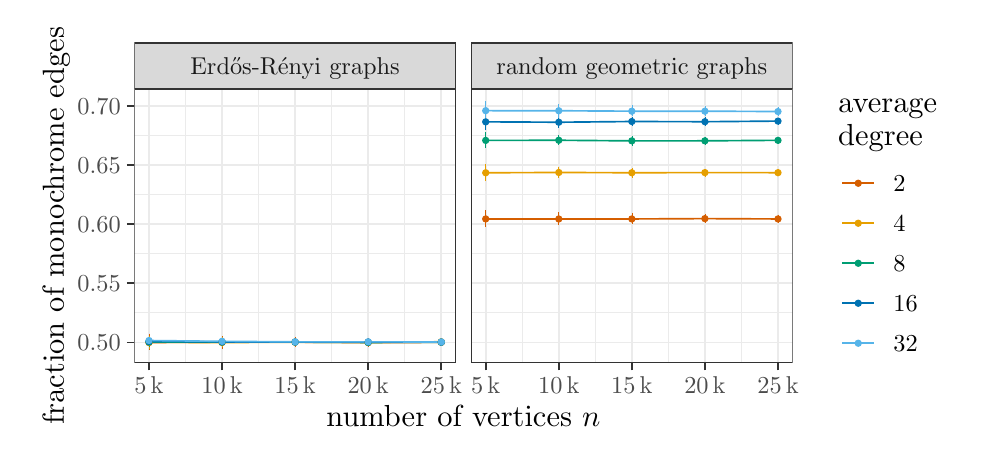
\begin{tikzpicture}[x=1pt,y=1pt]
\definecolor{fillColor}{RGB}{255,255,255}
\path[use as bounding box,fill=fillColor,fill opacity=0.00] (0,0) rectangle (339.67,151.77);
\begin{scope}
\path[clip] (  0.00,  0.00) rectangle (339.67,151.77);
\definecolor{drawColor}{RGB}{255,255,255}
\definecolor{fillColor}{RGB}{255,255,255}

\path[draw=drawColor,line width= 0.6pt,line join=round,line cap=round,fill=fillColor] (  0.00,  0.00) rectangle (339.67,151.77);
\end{scope}
\begin{scope}
\path[clip] ( 38.56, 30.69) rectangle (154.73,129.70);
\definecolor{fillColor}{RGB}{255,255,255}

\path[fill=fillColor] ( 38.56, 30.69) rectangle (154.73,129.70);
\definecolor{drawColor}{gray}{0.92}

\path[draw=drawColor,line width= 0.3pt,line join=round] ( 38.56, 48.75) --
	(154.73, 48.75);

\path[draw=drawColor,line width= 0.3pt,line join=round] ( 38.56, 70.12) --
	(154.73, 70.12);

\path[draw=drawColor,line width= 0.3pt,line join=round] ( 38.56, 91.49) --
	(154.73, 91.49);

\path[draw=drawColor,line width= 0.3pt,line join=round] ( 38.56,112.87) --
	(154.73,112.87);

\path[draw=drawColor,line width= 0.3pt,line join=round] ( 57.04, 30.69) --
	( 57.04,129.70);

\path[draw=drawColor,line width= 0.3pt,line join=round] ( 83.44, 30.69) --
	( 83.44,129.70);

\path[draw=drawColor,line width= 0.3pt,line join=round] (109.84, 30.69) --
	(109.84,129.70);

\path[draw=drawColor,line width= 0.3pt,line join=round] (136.24, 30.69) --
	(136.24,129.70);

\path[draw=drawColor,line width= 0.6pt,line join=round] ( 38.56, 38.06) --
	(154.73, 38.06);

\path[draw=drawColor,line width= 0.6pt,line join=round] ( 38.56, 59.43) --
	(154.73, 59.43);

\path[draw=drawColor,line width= 0.6pt,line join=round] ( 38.56, 80.81) --
	(154.73, 80.81);

\path[draw=drawColor,line width= 0.6pt,line join=round] ( 38.56,102.18) --
	(154.73,102.18);

\path[draw=drawColor,line width= 0.6pt,line join=round] ( 38.56,123.55) --
	(154.73,123.55);

\path[draw=drawColor,line width= 0.6pt,line join=round] ( 43.84, 30.69) --
	( 43.84,129.70);

\path[draw=drawColor,line width= 0.6pt,line join=round] ( 70.24, 30.69) --
	( 70.24,129.70);

\path[draw=drawColor,line width= 0.6pt,line join=round] ( 96.64, 30.69) --
	( 96.64,129.70);

\path[draw=drawColor,line width= 0.6pt,line join=round] (123.04, 30.69) --
	(123.04,129.70);

\path[draw=drawColor,line width= 0.6pt,line join=round] (149.45, 30.69) --
	(149.45,129.70);
\definecolor{drawColor}{RGB}{213,94,0}

\path[draw=drawColor,line width= 0.2pt,line join=round] ( 43.84, 41.18) --
	( 43.84, 41.18);

\path[draw=drawColor,line width= 0.2pt,line join=round] ( 43.84, 41.18) --
	( 43.84, 35.19);

\path[draw=drawColor,line width= 0.2pt,line join=round] ( 43.84, 35.19) --
	( 43.84, 35.19);

\path[draw=drawColor,line width= 0.2pt,line join=round] ( 70.24, 40.20) --
	( 70.24, 40.20);

\path[draw=drawColor,line width= 0.2pt,line join=round] ( 70.24, 40.20) --
	( 70.24, 35.73);

\path[draw=drawColor,line width= 0.2pt,line join=round] ( 70.24, 35.73) --
	( 70.24, 35.73);

\path[draw=drawColor,line width= 0.2pt,line join=round] ( 96.64, 40.06) --
	( 96.64, 40.06);

\path[draw=drawColor,line width= 0.2pt,line join=round] ( 96.64, 40.06) --
	( 96.64, 36.22);

\path[draw=drawColor,line width= 0.2pt,line join=round] ( 96.64, 36.22) --
	( 96.64, 36.22);

\path[draw=drawColor,line width= 0.2pt,line join=round] (123.04, 39.63) --
	(123.04, 39.63);

\path[draw=drawColor,line width= 0.2pt,line join=round] (123.04, 39.63) --
	(123.04, 36.40);

\path[draw=drawColor,line width= 0.2pt,line join=round] (123.04, 36.40) --
	(123.04, 36.40);

\path[draw=drawColor,line width= 0.2pt,line join=round] (149.45, 39.51) --
	(149.45, 39.51);

\path[draw=drawColor,line width= 0.2pt,line join=round] (149.45, 39.51) --
	(149.45, 36.61);

\path[draw=drawColor,line width= 0.2pt,line join=round] (149.45, 36.61) --
	(149.45, 36.61);
\definecolor{drawColor}{RGB}{230,159,0}

\path[draw=drawColor,line width= 0.2pt,line join=round] ( 43.84, 40.35) --
	( 43.84, 40.35);

\path[draw=drawColor,line width= 0.2pt,line join=round] ( 43.84, 40.35) --
	( 43.84, 35.56);

\path[draw=drawColor,line width= 0.2pt,line join=round] ( 43.84, 35.56) --
	( 43.84, 35.56);

\path[draw=drawColor,line width= 0.2pt,line join=round] ( 70.24, 39.84) --
	( 70.24, 39.84);

\path[draw=drawColor,line width= 0.2pt,line join=round] ( 70.24, 39.84) --
	( 70.24, 36.32);

\path[draw=drawColor,line width= 0.2pt,line join=round] ( 70.24, 36.32) --
	( 70.24, 36.32);

\path[draw=drawColor,line width= 0.2pt,line join=round] ( 96.64, 39.40) --
	( 96.64, 39.40);

\path[draw=drawColor,line width= 0.2pt,line join=round] ( 96.64, 39.40) --
	( 96.64, 36.67);

\path[draw=drawColor,line width= 0.2pt,line join=round] ( 96.64, 36.67) --
	( 96.64, 36.67);

\path[draw=drawColor,line width= 0.2pt,line join=round] (123.04, 39.23) --
	(123.04, 39.23);

\path[draw=drawColor,line width= 0.2pt,line join=round] (123.04, 39.23) --
	(123.04, 37.02);

\path[draw=drawColor,line width= 0.2pt,line join=round] (123.04, 37.02) --
	(123.04, 37.02);

\path[draw=drawColor,line width= 0.2pt,line join=round] (149.45, 39.25) --
	(149.45, 39.25);

\path[draw=drawColor,line width= 0.2pt,line join=round] (149.45, 39.25) --
	(149.45, 37.13);

\path[draw=drawColor,line width= 0.2pt,line join=round] (149.45, 37.13) --
	(149.45, 37.13);
\definecolor{drawColor}{RGB}{0,158,115}

\path[draw=drawColor,line width= 0.2pt,line join=round] ( 43.84, 40.11) --
	( 43.84, 40.11);

\path[draw=drawColor,line width= 0.2pt,line join=round] ( 43.84, 40.11) --
	( 43.84, 36.46);

\path[draw=drawColor,line width= 0.2pt,line join=round] ( 43.84, 36.46) --
	( 43.84, 36.46);

\path[draw=drawColor,line width= 0.2pt,line join=round] ( 70.24, 39.49) --
	( 70.24, 39.49);

\path[draw=drawColor,line width= 0.2pt,line join=round] ( 70.24, 39.49) --
	( 70.24, 36.95);

\path[draw=drawColor,line width= 0.2pt,line join=round] ( 70.24, 36.95) --
	( 70.24, 36.95);

\path[draw=drawColor,line width= 0.2pt,line join=round] ( 96.64, 39.15) --
	( 96.64, 39.15);

\path[draw=drawColor,line width= 0.2pt,line join=round] ( 96.64, 39.15) --
	( 96.64, 37.13);

\path[draw=drawColor,line width= 0.2pt,line join=round] ( 96.64, 37.13) --
	( 96.64, 37.13);

\path[draw=drawColor,line width= 0.2pt,line join=round] (123.04, 38.99) --
	(123.04, 38.99);

\path[draw=drawColor,line width= 0.2pt,line join=round] (123.04, 38.99) --
	(123.04, 37.14);

\path[draw=drawColor,line width= 0.2pt,line join=round] (123.04, 37.14) --
	(123.04, 37.14);

\path[draw=drawColor,line width= 0.2pt,line join=round] (149.45, 38.85) --
	(149.45, 38.85);

\path[draw=drawColor,line width= 0.2pt,line join=round] (149.45, 38.85) --
	(149.45, 37.33);

\path[draw=drawColor,line width= 0.2pt,line join=round] (149.45, 37.33) --
	(149.45, 37.33);
\definecolor{drawColor}{RGB}{0,114,178}

\path[draw=drawColor,line width= 0.2pt,line join=round] ( 43.84, 39.76) --
	( 43.84, 39.76);

\path[draw=drawColor,line width= 0.2pt,line join=round] ( 43.84, 39.76) --
	( 43.84, 37.04);

\path[draw=drawColor,line width= 0.2pt,line join=round] ( 43.84, 37.04) --
	( 43.84, 37.04);

\path[draw=drawColor,line width= 0.2pt,line join=round] ( 70.24, 39.10) --
	( 70.24, 39.10);

\path[draw=drawColor,line width= 0.2pt,line join=round] ( 70.24, 39.10) --
	( 70.24, 37.39);

\path[draw=drawColor,line width= 0.2pt,line join=round] ( 70.24, 37.39) --
	( 70.24, 37.39);

\path[draw=drawColor,line width= 0.2pt,line join=round] ( 96.64, 38.92) --
	( 96.64, 38.92);

\path[draw=drawColor,line width= 0.2pt,line join=round] ( 96.64, 38.92) --
	( 96.64, 37.46);

\path[draw=drawColor,line width= 0.2pt,line join=round] ( 96.64, 37.46) --
	( 96.64, 37.46);

\path[draw=drawColor,line width= 0.2pt,line join=round] (123.04, 38.84) --
	(123.04, 38.84);

\path[draw=drawColor,line width= 0.2pt,line join=round] (123.04, 38.84) --
	(123.04, 37.53);

\path[draw=drawColor,line width= 0.2pt,line join=round] (123.04, 37.53) --
	(123.04, 37.53);

\path[draw=drawColor,line width= 0.2pt,line join=round] (149.45, 38.75) --
	(149.45, 38.75);

\path[draw=drawColor,line width= 0.2pt,line join=round] (149.45, 38.75) --
	(149.45, 37.58);

\path[draw=drawColor,line width= 0.2pt,line join=round] (149.45, 37.58) --
	(149.45, 37.58);
\definecolor{drawColor}{RGB}{86,180,233}

\path[draw=drawColor,line width= 0.2pt,line join=round] ( 43.84, 39.94) --
	( 43.84, 39.94);

\path[draw=drawColor,line width= 0.2pt,line join=round] ( 43.84, 39.94) --
	( 43.84, 37.63);

\path[draw=drawColor,line width= 0.2pt,line join=round] ( 43.84, 37.63) --
	( 43.84, 37.63);

\path[draw=drawColor,line width= 0.2pt,line join=round] ( 70.24, 39.17) --
	( 70.24, 39.17);

\path[draw=drawColor,line width= 0.2pt,line join=round] ( 70.24, 39.17) --
	( 70.24, 37.75);

\path[draw=drawColor,line width= 0.2pt,line join=round] ( 70.24, 37.75) --
	( 70.24, 37.75);

\path[draw=drawColor,line width= 0.2pt,line join=round] ( 96.64, 38.86) --
	( 96.64, 38.86);

\path[draw=drawColor,line width= 0.2pt,line join=round] ( 96.64, 38.86) --
	( 96.64, 37.75);

\path[draw=drawColor,line width= 0.2pt,line join=round] ( 96.64, 37.75) --
	( 96.64, 37.75);

\path[draw=drawColor,line width= 0.2pt,line join=round] (123.04, 38.76) --
	(123.04, 38.76);

\path[draw=drawColor,line width= 0.2pt,line join=round] (123.04, 38.76) --
	(123.04, 37.74);

\path[draw=drawColor,line width= 0.2pt,line join=round] (123.04, 37.74) --
	(123.04, 37.74);

\path[draw=drawColor,line width= 0.2pt,line join=round] (149.45, 38.63) --
	(149.45, 38.63);

\path[draw=drawColor,line width= 0.2pt,line join=round] (149.45, 38.63) --
	(149.45, 37.79);

\path[draw=drawColor,line width= 0.2pt,line join=round] (149.45, 37.79) --
	(149.45, 37.79);
\definecolor{drawColor}{RGB}{213,94,0}

\path[draw=drawColor,line width= 0.6pt,line join=round] ( 43.84, 38.00) --
	( 70.24, 38.15) --
	( 96.64, 38.15) --
	(123.04, 37.97) --
	(149.45, 38.06);
\definecolor{drawColor}{RGB}{230,159,0}

\path[draw=drawColor,line width= 0.6pt,line join=round] ( 43.84, 38.10) --
	( 70.24, 37.98) --
	( 96.64, 38.13) --
	(123.04, 38.06) --
	(149.45, 38.27);
\definecolor{drawColor}{RGB}{0,158,115}

\path[draw=drawColor,line width= 0.6pt,line join=round] ( 43.84, 38.17) --
	( 70.24, 38.17) --
	( 96.64, 38.16) --
	(123.04, 38.02) --
	(149.45, 38.10);
\definecolor{drawColor}{RGB}{0,114,178}

\path[draw=drawColor,line width= 0.6pt,line join=round] ( 43.84, 38.40) --
	( 70.24, 38.20) --
	( 96.64, 38.17) --
	(123.04, 38.21) --
	(149.45, 38.17);
\definecolor{drawColor}{RGB}{86,180,233}

\path[draw=drawColor,line width= 0.6pt,line join=round] ( 43.84, 38.72) --
	( 70.24, 38.43) --
	( 96.64, 38.24) --
	(123.04, 38.24) --
	(149.45, 38.19);
\definecolor{drawColor}{RGB}{213,94,0}
\definecolor{fillColor}{RGB}{213,94,0}

\path[draw=drawColor,line width= 0.4pt,line join=round,line cap=round,fill=fillColor] ( 43.84, 38.00) circle (  1.11);

\path[draw=drawColor,line width= 0.4pt,line join=round,line cap=round,fill=fillColor] ( 70.24, 38.15) circle (  1.11);

\path[draw=drawColor,line width= 0.4pt,line join=round,line cap=round,fill=fillColor] ( 96.64, 38.15) circle (  1.11);

\path[draw=drawColor,line width= 0.4pt,line join=round,line cap=round,fill=fillColor] (123.04, 37.97) circle (  1.11);

\path[draw=drawColor,line width= 0.4pt,line join=round,line cap=round,fill=fillColor] (149.45, 38.06) circle (  1.11);
\definecolor{drawColor}{RGB}{230,159,0}
\definecolor{fillColor}{RGB}{230,159,0}

\path[draw=drawColor,line width= 0.4pt,line join=round,line cap=round,fill=fillColor] ( 43.84, 38.10) circle (  1.11);

\path[draw=drawColor,line width= 0.4pt,line join=round,line cap=round,fill=fillColor] ( 70.24, 37.98) circle (  1.11);

\path[draw=drawColor,line width= 0.4pt,line join=round,line cap=round,fill=fillColor] ( 96.64, 38.13) circle (  1.11);

\path[draw=drawColor,line width= 0.4pt,line join=round,line cap=round,fill=fillColor] (123.04, 38.06) circle (  1.11);

\path[draw=drawColor,line width= 0.4pt,line join=round,line cap=round,fill=fillColor] (149.45, 38.27) circle (  1.11);
\definecolor{drawColor}{RGB}{0,158,115}
\definecolor{fillColor}{RGB}{0,158,115}

\path[draw=drawColor,line width= 0.4pt,line join=round,line cap=round,fill=fillColor] ( 43.84, 38.17) circle (  1.11);

\path[draw=drawColor,line width= 0.4pt,line join=round,line cap=round,fill=fillColor] ( 70.24, 38.17) circle (  1.11);

\path[draw=drawColor,line width= 0.4pt,line join=round,line cap=round,fill=fillColor] ( 96.64, 38.16) circle (  1.11);

\path[draw=drawColor,line width= 0.4pt,line join=round,line cap=round,fill=fillColor] (123.04, 38.02) circle (  1.11);

\path[draw=drawColor,line width= 0.4pt,line join=round,line cap=round,fill=fillColor] (149.45, 38.10) circle (  1.11);
\definecolor{drawColor}{RGB}{0,114,178}
\definecolor{fillColor}{RGB}{0,114,178}

\path[draw=drawColor,line width= 0.4pt,line join=round,line cap=round,fill=fillColor] ( 43.84, 38.40) circle (  1.11);

\path[draw=drawColor,line width= 0.4pt,line join=round,line cap=round,fill=fillColor] ( 70.24, 38.20) circle (  1.11);

\path[draw=drawColor,line width= 0.4pt,line join=round,line cap=round,fill=fillColor] ( 96.64, 38.17) circle (  1.11);

\path[draw=drawColor,line width= 0.4pt,line join=round,line cap=round,fill=fillColor] (123.04, 38.21) circle (  1.11);

\path[draw=drawColor,line width= 0.4pt,line join=round,line cap=round,fill=fillColor] (149.45, 38.17) circle (  1.11);
\definecolor{drawColor}{RGB}{86,180,233}
\definecolor{fillColor}{RGB}{86,180,233}

\path[draw=drawColor,line width= 0.4pt,line join=round,line cap=round,fill=fillColor] ( 43.84, 38.72) circle (  1.11);

\path[draw=drawColor,line width= 0.4pt,line join=round,line cap=round,fill=fillColor] ( 70.24, 38.43) circle (  1.11);

\path[draw=drawColor,line width= 0.4pt,line join=round,line cap=round,fill=fillColor] ( 96.64, 38.24) circle (  1.11);

\path[draw=drawColor,line width= 0.4pt,line join=round,line cap=round,fill=fillColor] (123.04, 38.24) circle (  1.11);

\path[draw=drawColor,line width= 0.4pt,line join=round,line cap=round,fill=fillColor] (149.45, 38.19) circle (  1.11);
\definecolor{drawColor}{gray}{0.20}

\path[draw=drawColor,line width= 0.6pt,line join=round,line cap=round] ( 38.56, 30.69) rectangle (154.73,129.70);
\end{scope}
\begin{scope}
\path[clip] (160.23, 30.69) rectangle (276.40,129.70);
\definecolor{fillColor}{RGB}{255,255,255}

\path[fill=fillColor] (160.23, 30.69) rectangle (276.40,129.70);
\definecolor{drawColor}{gray}{0.92}

\path[draw=drawColor,line width= 0.3pt,line join=round] (160.23, 48.75) --
	(276.40, 48.75);

\path[draw=drawColor,line width= 0.3pt,line join=round] (160.23, 70.12) --
	(276.40, 70.12);

\path[draw=drawColor,line width= 0.3pt,line join=round] (160.23, 91.49) --
	(276.40, 91.49);

\path[draw=drawColor,line width= 0.3pt,line join=round] (160.23,112.87) --
	(276.40,112.87);

\path[draw=drawColor,line width= 0.3pt,line join=round] (178.71, 30.69) --
	(178.71,129.70);

\path[draw=drawColor,line width= 0.3pt,line join=round] (205.11, 30.69) --
	(205.11,129.70);

\path[draw=drawColor,line width= 0.3pt,line join=round] (231.51, 30.69) --
	(231.51,129.70);

\path[draw=drawColor,line width= 0.3pt,line join=round] (257.92, 30.69) --
	(257.92,129.70);

\path[draw=drawColor,line width= 0.6pt,line join=round] (160.23, 38.06) --
	(276.40, 38.06);

\path[draw=drawColor,line width= 0.6pt,line join=round] (160.23, 59.43) --
	(276.40, 59.43);

\path[draw=drawColor,line width= 0.6pt,line join=round] (160.23, 80.81) --
	(276.40, 80.81);

\path[draw=drawColor,line width= 0.6pt,line join=round] (160.23,102.18) --
	(276.40,102.18);

\path[draw=drawColor,line width= 0.6pt,line join=round] (160.23,123.55) --
	(276.40,123.55);

\path[draw=drawColor,line width= 0.6pt,line join=round] (165.51, 30.69) --
	(165.51,129.70);

\path[draw=drawColor,line width= 0.6pt,line join=round] (191.91, 30.69) --
	(191.91,129.70);

\path[draw=drawColor,line width= 0.6pt,line join=round] (218.31, 30.69) --
	(218.31,129.70);

\path[draw=drawColor,line width= 0.6pt,line join=round] (244.71, 30.69) --
	(244.71,129.70);

\path[draw=drawColor,line width= 0.6pt,line join=round] (271.12, 30.69) --
	(271.12,129.70);
\definecolor{drawColor}{RGB}{213,94,0}

\path[draw=drawColor,line width= 0.2pt,line join=round] (165.51, 85.78) --
	(165.51, 85.78);

\path[draw=drawColor,line width= 0.2pt,line join=round] (165.51, 85.78) --
	(165.51, 79.76);

\path[draw=drawColor,line width= 0.2pt,line join=round] (165.51, 79.76) --
	(165.51, 79.76);

\path[draw=drawColor,line width= 0.2pt,line join=round] (191.91, 85.13) --
	(191.91, 85.13);

\path[draw=drawColor,line width= 0.2pt,line join=round] (191.91, 85.13) --
	(191.91, 80.35);

\path[draw=drawColor,line width= 0.2pt,line join=round] (191.91, 80.35) --
	(191.91, 80.35);

\path[draw=drawColor,line width= 0.2pt,line join=round] (218.31, 84.81) --
	(218.31, 84.81);

\path[draw=drawColor,line width= 0.2pt,line join=round] (218.31, 84.81) --
	(218.31, 80.69);

\path[draw=drawColor,line width= 0.2pt,line join=round] (218.31, 80.69) --
	(218.31, 80.69);

\path[draw=drawColor,line width= 0.2pt,line join=round] (244.71, 84.49) --
	(244.71, 84.49);

\path[draw=drawColor,line width= 0.2pt,line join=round] (244.71, 84.49) --
	(244.71, 81.04);

\path[draw=drawColor,line width= 0.2pt,line join=round] (244.71, 81.04) --
	(244.71, 81.04);

\path[draw=drawColor,line width= 0.2pt,line join=round] (271.12, 84.18) --
	(271.12, 84.18);

\path[draw=drawColor,line width= 0.2pt,line join=round] (271.12, 84.18) --
	(271.12, 81.16);

\path[draw=drawColor,line width= 0.2pt,line join=round] (271.12, 81.16) --
	(271.12, 81.16);
\definecolor{drawColor}{RGB}{230,159,0}

\path[draw=drawColor,line width= 0.2pt,line join=round] (165.51,102.33) --
	(165.51,102.33);

\path[draw=drawColor,line width= 0.2pt,line join=round] (165.51,102.33) --
	(165.51, 96.43);

\path[draw=drawColor,line width= 0.2pt,line join=round] (165.51, 96.43) --
	(165.51, 96.43);

\path[draw=drawColor,line width= 0.2pt,line join=round] (191.91,101.44) --
	(191.91,101.44);

\path[draw=drawColor,line width= 0.2pt,line join=round] (191.91,101.44) --
	(191.91, 97.33);

\path[draw=drawColor,line width= 0.2pt,line join=round] (191.91, 97.33) --
	(191.91, 97.33);

\path[draw=drawColor,line width= 0.2pt,line join=round] (218.31,101.05) --
	(218.31,101.05);

\path[draw=drawColor,line width= 0.2pt,line join=round] (218.31,101.05) --
	(218.31, 97.61);

\path[draw=drawColor,line width= 0.2pt,line join=round] (218.31, 97.61) --
	(218.31, 97.61);

\path[draw=drawColor,line width= 0.2pt,line join=round] (244.71,100.83) --
	(244.71,100.83);

\path[draw=drawColor,line width= 0.2pt,line join=round] (244.71,100.83) --
	(244.71, 97.88);

\path[draw=drawColor,line width= 0.2pt,line join=round] (244.71, 97.88) --
	(244.71, 97.88);

\path[draw=drawColor,line width= 0.2pt,line join=round] (271.12,100.74) --
	(271.12,100.74);

\path[draw=drawColor,line width= 0.2pt,line join=round] (271.12,100.74) --
	(271.12, 98.06);

\path[draw=drawColor,line width= 0.2pt,line join=round] (271.12, 98.06) --
	(271.12, 98.06);
\definecolor{drawColor}{RGB}{0,158,115}

\path[draw=drawColor,line width= 0.2pt,line join=round] (165.51,113.91) --
	(165.51,113.91);

\path[draw=drawColor,line width= 0.2pt,line join=round] (165.51,113.91) --
	(165.51,108.44);

\path[draw=drawColor,line width= 0.2pt,line join=round] (165.51,108.44) --
	(165.51,108.44);

\path[draw=drawColor,line width= 0.2pt,line join=round] (191.91,112.99) --
	(191.91,112.99);

\path[draw=drawColor,line width= 0.2pt,line join=round] (191.91,112.99) --
	(191.91,109.30);

\path[draw=drawColor,line width= 0.2pt,line join=round] (191.91,109.30) --
	(191.91,109.30);

\path[draw=drawColor,line width= 0.2pt,line join=round] (218.31,112.68) --
	(218.31,112.68);

\path[draw=drawColor,line width= 0.2pt,line join=round] (218.31,112.68) --
	(218.31,109.14);

\path[draw=drawColor,line width= 0.2pt,line join=round] (218.31,109.14) --
	(218.31,109.14);

\path[draw=drawColor,line width= 0.2pt,line join=round] (244.71,112.34) --
	(244.71,112.34);

\path[draw=drawColor,line width= 0.2pt,line join=round] (244.71,112.34) --
	(244.71,109.46);

\path[draw=drawColor,line width= 0.2pt,line join=round] (244.71,109.46) --
	(244.71,109.46);

\path[draw=drawColor,line width= 0.2pt,line join=round] (271.12,112.22) --
	(271.12,112.22);

\path[draw=drawColor,line width= 0.2pt,line join=round] (271.12,112.22) --
	(271.12,109.83);

\path[draw=drawColor,line width= 0.2pt,line join=round] (271.12,109.83) --
	(271.12,109.83);
\definecolor{drawColor}{RGB}{0,114,178}

\path[draw=drawColor,line width= 0.2pt,line join=round] (165.51,120.41) --
	(165.51,120.41);

\path[draw=drawColor,line width= 0.2pt,line join=round] (165.51,120.41) --
	(165.51,114.77);

\path[draw=drawColor,line width= 0.2pt,line join=round] (165.51,114.77) --
	(165.51,114.77);

\path[draw=drawColor,line width= 0.2pt,line join=round] (191.91,119.84) --
	(191.91,119.84);

\path[draw=drawColor,line width= 0.2pt,line join=round] (191.91,119.84) --
	(191.91,115.64);

\path[draw=drawColor,line width= 0.2pt,line join=round] (191.91,115.64) --
	(191.91,115.64);

\path[draw=drawColor,line width= 0.2pt,line join=round] (218.31,119.47) --
	(218.31,119.47);

\path[draw=drawColor,line width= 0.2pt,line join=round] (218.31,119.47) --
	(218.31,116.09);

\path[draw=drawColor,line width= 0.2pt,line join=round] (218.31,116.09) --
	(218.31,116.09);

\path[draw=drawColor,line width= 0.2pt,line join=round] (244.71,119.31) --
	(244.71,119.31);

\path[draw=drawColor,line width= 0.2pt,line join=round] (244.71,119.31) --
	(244.71,116.35);

\path[draw=drawColor,line width= 0.2pt,line join=round] (244.71,116.35) --
	(244.71,116.35);

\path[draw=drawColor,line width= 0.2pt,line join=round] (271.12,119.25) --
	(271.12,119.25);

\path[draw=drawColor,line width= 0.2pt,line join=round] (271.12,119.25) --
	(271.12,116.71);

\path[draw=drawColor,line width= 0.2pt,line join=round] (271.12,116.71) --
	(271.12,116.71);
\definecolor{drawColor}{RGB}{86,180,233}

\path[draw=drawColor,line width= 0.2pt,line join=round] (165.51,125.20) --
	(165.51,125.20);

\path[draw=drawColor,line width= 0.2pt,line join=round] (165.51,125.20) --
	(165.51,118.34);

\path[draw=drawColor,line width= 0.2pt,line join=round] (165.51,118.34) --
	(165.51,118.34);

\path[draw=drawColor,line width= 0.2pt,line join=round] (191.91,124.06) --
	(191.91,124.06);

\path[draw=drawColor,line width= 0.2pt,line join=round] (191.91,124.06) --
	(191.91,119.29);

\path[draw=drawColor,line width= 0.2pt,line join=round] (191.91,119.29) --
	(191.91,119.29);

\path[draw=drawColor,line width= 0.2pt,line join=round] (218.31,123.77) --
	(218.31,123.77);

\path[draw=drawColor,line width= 0.2pt,line join=round] (218.31,123.77) --
	(218.31,119.69);

\path[draw=drawColor,line width= 0.2pt,line join=round] (218.31,119.69) --
	(218.31,119.69);

\path[draw=drawColor,line width= 0.2pt,line join=round] (244.71,123.34) --
	(244.71,123.34);

\path[draw=drawColor,line width= 0.2pt,line join=round] (244.71,123.34) --
	(244.71,119.81);

\path[draw=drawColor,line width= 0.2pt,line join=round] (244.71,119.81) --
	(244.71,119.81);

\path[draw=drawColor,line width= 0.2pt,line join=round] (271.12,123.03) --
	(271.12,123.03);

\path[draw=drawColor,line width= 0.2pt,line join=round] (271.12,123.03) --
	(271.12,119.85);

\path[draw=drawColor,line width= 0.2pt,line join=round] (271.12,119.85) --
	(271.12,119.85);
\definecolor{drawColor}{RGB}{213,94,0}

\path[draw=drawColor,line width= 0.6pt,line join=round] (165.51, 82.66) --
	(191.91, 82.64) --
	(218.31, 82.65) --
	(244.71, 82.77) --
	(271.12, 82.65);
\definecolor{drawColor}{RGB}{230,159,0}

\path[draw=drawColor,line width= 0.6pt,line join=round] (165.51, 99.34) --
	(191.91, 99.44) --
	(218.31, 99.35) --
	(244.71, 99.40) --
	(271.12, 99.37);
\definecolor{drawColor}{RGB}{0,158,115}

\path[draw=drawColor,line width= 0.6pt,line join=round] (165.51,111.03) --
	(191.91,111.08) --
	(218.31,110.87) --
	(244.71,110.88) --
	(271.12,111.06);
\definecolor{drawColor}{RGB}{0,114,178}

\path[draw=drawColor,line width= 0.6pt,line join=round] (165.51,117.74) --
	(191.91,117.60) --
	(218.31,117.86) --
	(244.71,117.79) --
	(271.12,118.01);
\definecolor{drawColor}{RGB}{86,180,233}

\path[draw=drawColor,line width= 0.6pt,line join=round] (165.51,121.78) --
	(191.91,121.75) --
	(218.31,121.59) --
	(244.71,121.59) --
	(271.12,121.47);
\definecolor{drawColor}{RGB}{213,94,0}
\definecolor{fillColor}{RGB}{213,94,0}

\path[draw=drawColor,line width= 0.4pt,line join=round,line cap=round,fill=fillColor] (165.51, 82.66) circle (  1.11);

\path[draw=drawColor,line width= 0.4pt,line join=round,line cap=round,fill=fillColor] (191.91, 82.64) circle (  1.11);

\path[draw=drawColor,line width= 0.4pt,line join=round,line cap=round,fill=fillColor] (218.31, 82.65) circle (  1.11);

\path[draw=drawColor,line width= 0.4pt,line join=round,line cap=round,fill=fillColor] (244.71, 82.77) circle (  1.11);

\path[draw=drawColor,line width= 0.4pt,line join=round,line cap=round,fill=fillColor] (271.12, 82.65) circle (  1.11);
\definecolor{drawColor}{RGB}{230,159,0}
\definecolor{fillColor}{RGB}{230,159,0}

\path[draw=drawColor,line width= 0.4pt,line join=round,line cap=round,fill=fillColor] (165.51, 99.34) circle (  1.11);

\path[draw=drawColor,line width= 0.4pt,line join=round,line cap=round,fill=fillColor] (191.91, 99.44) circle (  1.11);

\path[draw=drawColor,line width= 0.4pt,line join=round,line cap=round,fill=fillColor] (218.31, 99.35) circle (  1.11);

\path[draw=drawColor,line width= 0.4pt,line join=round,line cap=round,fill=fillColor] (244.71, 99.40) circle (  1.11);

\path[draw=drawColor,line width= 0.4pt,line join=round,line cap=round,fill=fillColor] (271.12, 99.37) circle (  1.11);
\definecolor{drawColor}{RGB}{0,158,115}
\definecolor{fillColor}{RGB}{0,158,115}

\path[draw=drawColor,line width= 0.4pt,line join=round,line cap=round,fill=fillColor] (165.51,111.03) circle (  1.11);

\path[draw=drawColor,line width= 0.4pt,line join=round,line cap=round,fill=fillColor] (191.91,111.08) circle (  1.11);

\path[draw=drawColor,line width= 0.4pt,line join=round,line cap=round,fill=fillColor] (218.31,110.87) circle (  1.11);

\path[draw=drawColor,line width= 0.4pt,line join=round,line cap=round,fill=fillColor] (244.71,110.88) circle (  1.11);

\path[draw=drawColor,line width= 0.4pt,line join=round,line cap=round,fill=fillColor] (271.12,111.06) circle (  1.11);
\definecolor{drawColor}{RGB}{0,114,178}
\definecolor{fillColor}{RGB}{0,114,178}

\path[draw=drawColor,line width= 0.4pt,line join=round,line cap=round,fill=fillColor] (165.51,117.74) circle (  1.11);

\path[draw=drawColor,line width= 0.4pt,line join=round,line cap=round,fill=fillColor] (191.91,117.60) circle (  1.11);

\path[draw=drawColor,line width= 0.4pt,line join=round,line cap=round,fill=fillColor] (218.31,117.86) circle (  1.11);

\path[draw=drawColor,line width= 0.4pt,line join=round,line cap=round,fill=fillColor] (244.71,117.79) circle (  1.11);

\path[draw=drawColor,line width= 0.4pt,line join=round,line cap=round,fill=fillColor] (271.12,118.01) circle (  1.11);
\definecolor{drawColor}{RGB}{86,180,233}
\definecolor{fillColor}{RGB}{86,180,233}

\path[draw=drawColor,line width= 0.4pt,line join=round,line cap=round,fill=fillColor] (165.51,121.78) circle (  1.11);

\path[draw=drawColor,line width= 0.4pt,line join=round,line cap=round,fill=fillColor] (191.91,121.75) circle (  1.11);

\path[draw=drawColor,line width= 0.4pt,line join=round,line cap=round,fill=fillColor] (218.31,121.59) circle (  1.11);

\path[draw=drawColor,line width= 0.4pt,line join=round,line cap=round,fill=fillColor] (244.71,121.59) circle (  1.11);

\path[draw=drawColor,line width= 0.4pt,line join=round,line cap=round,fill=fillColor] (271.12,121.47) circle (  1.11);
\definecolor{drawColor}{gray}{0.20}

\path[draw=drawColor,line width= 0.6pt,line join=round,line cap=round] (160.23, 30.69) rectangle (276.40,129.70);
\end{scope}
\begin{scope}
\path[clip] ( 38.56,129.70) rectangle (154.73,146.27);
\definecolor{drawColor}{gray}{0.20}
\definecolor{fillColor}{gray}{0.85}

\path[draw=drawColor,line width= 0.6pt,line join=round,line cap=round,fill=fillColor] ( 38.56,129.70) rectangle (154.73,146.27);
\definecolor{drawColor}{gray}{0.10}

\node[text=drawColor,anchor=base,inner sep=0pt, outer sep=0pt, scale=  0.88] at ( 96.64,134.95) {Erd{\H o}s-R\'enyi graphs};
\end{scope}
\begin{scope}
\path[clip] (160.23,129.70) rectangle (276.40,146.27);
\definecolor{drawColor}{gray}{0.20}
\definecolor{fillColor}{gray}{0.85}

\path[draw=drawColor,line width= 0.6pt,line join=round,line cap=round,fill=fillColor] (160.23,129.70) rectangle (276.40,146.27);
\definecolor{drawColor}{gray}{0.10}

\node[text=drawColor,anchor=base,inner sep=0pt, outer sep=0pt, scale=  0.88] at (218.31,134.95) {random geometric graphs};
\end{scope}
\begin{scope}
\path[clip] (  0.00,  0.00) rectangle (339.67,151.77);
\definecolor{drawColor}{gray}{0.20}

\path[draw=drawColor,line width= 0.6pt,line join=round] ( 43.84, 27.94) --
	( 43.84, 30.69);

\path[draw=drawColor,line width= 0.6pt,line join=round] ( 70.24, 27.94) --
	( 70.24, 30.69);

\path[draw=drawColor,line width= 0.6pt,line join=round] ( 96.64, 27.94) --
	( 96.64, 30.69);

\path[draw=drawColor,line width= 0.6pt,line join=round] (123.04, 27.94) --
	(123.04, 30.69);

\path[draw=drawColor,line width= 0.6pt,line join=round] (149.45, 27.94) --
	(149.45, 30.69);
\end{scope}
\begin{scope}
\path[clip] (  0.00,  0.00) rectangle (339.67,151.77);
\definecolor{drawColor}{gray}{0.30}

\node[text=drawColor,anchor=base,inner sep=0pt, outer sep=0pt, scale=  0.88] at ( 43.84, 19.68) {5\,k};

\node[text=drawColor,anchor=base,inner sep=0pt, outer sep=0pt, scale=  0.88] at ( 70.24, 19.68) {10\,k};

\node[text=drawColor,anchor=base,inner sep=0pt, outer sep=0pt, scale=  0.88] at ( 96.64, 19.68) {15\,k};

\node[text=drawColor,anchor=base,inner sep=0pt, outer sep=0pt, scale=  0.88] at (123.04, 19.68) {20\,k};

\node[text=drawColor,anchor=base,inner sep=0pt, outer sep=0pt, scale=  0.88] at (149.45, 19.68) {25\,k};
\end{scope}
\begin{scope}
\path[clip] (  0.00,  0.00) rectangle (339.67,151.77);
\definecolor{drawColor}{gray}{0.20}

\path[draw=drawColor,line width= 0.6pt,line join=round] (165.51, 27.94) --
	(165.51, 30.69);

\path[draw=drawColor,line width= 0.6pt,line join=round] (191.91, 27.94) --
	(191.91, 30.69);

\path[draw=drawColor,line width= 0.6pt,line join=round] (218.31, 27.94) --
	(218.31, 30.69);

\path[draw=drawColor,line width= 0.6pt,line join=round] (244.71, 27.94) --
	(244.71, 30.69);

\path[draw=drawColor,line width= 0.6pt,line join=round] (271.12, 27.94) --
	(271.12, 30.69);
\end{scope}
\begin{scope}
\path[clip] (  0.00,  0.00) rectangle (339.67,151.77);
\definecolor{drawColor}{gray}{0.30}

\node[text=drawColor,anchor=base,inner sep=0pt, outer sep=0pt, scale=  0.88] at (165.51, 19.68) {5\,k};

\node[text=drawColor,anchor=base,inner sep=0pt, outer sep=0pt, scale=  0.88] at (191.91, 19.68) {10\,k};

\node[text=drawColor,anchor=base,inner sep=0pt, outer sep=0pt, scale=  0.88] at (218.31, 19.68) {15\,k};

\node[text=drawColor,anchor=base,inner sep=0pt, outer sep=0pt, scale=  0.88] at (244.71, 19.68) {20\,k};

\node[text=drawColor,anchor=base,inner sep=0pt, outer sep=0pt, scale=  0.88] at (271.12, 19.68) {25\,k};
\end{scope}
\begin{scope}
\path[clip] (  0.00,  0.00) rectangle (339.67,151.77);
\definecolor{drawColor}{gray}{0.30}

\node[text=drawColor,anchor=base east,inner sep=0pt, outer sep=0pt, scale=  0.88] at ( 33.61, 35.03) {0.50};

\node[text=drawColor,anchor=base east,inner sep=0pt, outer sep=0pt, scale=  0.88] at ( 33.61, 56.40) {0.55};

\node[text=drawColor,anchor=base east,inner sep=0pt, outer sep=0pt, scale=  0.88] at ( 33.61, 77.78) {0.60};

\node[text=drawColor,anchor=base east,inner sep=0pt, outer sep=0pt, scale=  0.88] at ( 33.61, 99.15) {0.65};

\node[text=drawColor,anchor=base east,inner sep=0pt, outer sep=0pt, scale=  0.88] at ( 33.61,120.52) {0.70};
\end{scope}
\begin{scope}
\path[clip] (  0.00,  0.00) rectangle (339.67,151.77);
\definecolor{drawColor}{gray}{0.20}

\path[draw=drawColor,line width= 0.6pt,line join=round] ( 35.81, 38.06) --
	( 38.56, 38.06);

\path[draw=drawColor,line width= 0.6pt,line join=round] ( 35.81, 59.43) --
	( 38.56, 59.43);

\path[draw=drawColor,line width= 0.6pt,line join=round] ( 35.81, 80.81) --
	( 38.56, 80.81);

\path[draw=drawColor,line width= 0.6pt,line join=round] ( 35.81,102.18) --
	( 38.56,102.18);

\path[draw=drawColor,line width= 0.6pt,line join=round] ( 35.81,123.55) --
	( 38.56,123.55);
\end{scope}
\begin{scope}
\path[clip] (  0.00,  0.00) rectangle (339.67,151.77);
\definecolor{drawColor}{RGB}{0,0,0}

\node[text=drawColor,anchor=base,inner sep=0pt, outer sep=0pt, scale=  1.10] at (157.48,  7.64) {number of vertices $n$};
\end{scope}
\begin{scope}
\path[clip] (  0.00,  0.00) rectangle (339.67,151.77);
\definecolor{drawColor}{RGB}{0,0,0}

\node[text=drawColor,rotate= 90.00,anchor=base,inner sep=0pt, outer sep=0pt, scale=  1.10] at ( 13.08, 80.19) {fraction of monochrome edges};
\end{scope}
\begin{scope}
\path[clip] (  0.00,  0.00) rectangle (339.67,151.77);
\definecolor{fillColor}{RGB}{255,255,255}

\path[fill=fillColor] (287.40, 25.01) rectangle (334.17,135.37);
\end{scope}
\begin{scope}
\path[clip] (  0.00,  0.00) rectangle (339.67,151.77);
\definecolor{drawColor}{RGB}{0,0,0}

\node[text=drawColor,anchor=base west,inner sep=0pt, outer sep=0pt, scale=  1.10] at (292.90,121.23) {average};

\node[text=drawColor,anchor=base west,inner sep=0pt, outer sep=0pt, scale=  1.10] at (292.90,109.35) {degree};
\end{scope}
\begin{scope}
\path[clip] (  0.00,  0.00) rectangle (339.67,151.77);
\definecolor{fillColor}{RGB}{255,255,255}

\path[fill=fillColor] (292.90, 88.32) rectangle (307.35,102.78);
\end{scope}
\begin{scope}
\path[clip] (  0.00,  0.00) rectangle (339.67,151.77);
\definecolor{drawColor}{RGB}{213,94,0}

\path[draw=drawColor,line width= 0.2pt,line join=round] (294.34, 95.55) -- (305.91, 95.55);
\end{scope}
\begin{scope}
\path[clip] (  0.00,  0.00) rectangle (339.67,151.77);
\definecolor{drawColor}{RGB}{213,94,0}

\path[draw=drawColor,line width= 0.6pt,line join=round] (294.34, 95.55) -- (305.91, 95.55);
\end{scope}
\begin{scope}
\path[clip] (  0.00,  0.00) rectangle (339.67,151.77);
\definecolor{drawColor}{RGB}{213,94,0}
\definecolor{fillColor}{RGB}{213,94,0}

\path[draw=drawColor,line width= 0.4pt,line join=round,line cap=round,fill=fillColor] (300.12, 95.55) circle (  1.11);
\end{scope}
\begin{scope}
\path[clip] (  0.00,  0.00) rectangle (339.67,151.77);
\definecolor{fillColor}{RGB}{255,255,255}

\path[fill=fillColor] (292.90, 73.87) rectangle (307.35, 88.32);
\end{scope}
\begin{scope}
\path[clip] (  0.00,  0.00) rectangle (339.67,151.77);
\definecolor{drawColor}{RGB}{230,159,0}

\path[draw=drawColor,line width= 0.2pt,line join=round] (294.34, 81.10) -- (305.91, 81.10);
\end{scope}
\begin{scope}
\path[clip] (  0.00,  0.00) rectangle (339.67,151.77);
\definecolor{drawColor}{RGB}{230,159,0}

\path[draw=drawColor,line width= 0.6pt,line join=round] (294.34, 81.10) -- (305.91, 81.10);
\end{scope}
\begin{scope}
\path[clip] (  0.00,  0.00) rectangle (339.67,151.77);
\definecolor{drawColor}{RGB}{230,159,0}
\definecolor{fillColor}{RGB}{230,159,0}

\path[draw=drawColor,line width= 0.4pt,line join=round,line cap=round,fill=fillColor] (300.12, 81.10) circle (  1.11);
\end{scope}
\begin{scope}
\path[clip] (  0.00,  0.00) rectangle (339.67,151.77);
\definecolor{fillColor}{RGB}{255,255,255}

\path[fill=fillColor] (292.90, 59.42) rectangle (307.35, 73.87);
\end{scope}
\begin{scope}
\path[clip] (  0.00,  0.00) rectangle (339.67,151.77);
\definecolor{drawColor}{RGB}{0,158,115}

\path[draw=drawColor,line width= 0.2pt,line join=round] (294.34, 66.64) -- (305.91, 66.64);
\end{scope}
\begin{scope}
\path[clip] (  0.00,  0.00) rectangle (339.67,151.77);
\definecolor{drawColor}{RGB}{0,158,115}

\path[draw=drawColor,line width= 0.6pt,line join=round] (294.34, 66.64) -- (305.91, 66.64);
\end{scope}
\begin{scope}
\path[clip] (  0.00,  0.00) rectangle (339.67,151.77);
\definecolor{drawColor}{RGB}{0,158,115}
\definecolor{fillColor}{RGB}{0,158,115}

\path[draw=drawColor,line width= 0.4pt,line join=round,line cap=round,fill=fillColor] (300.12, 66.64) circle (  1.11);
\end{scope}
\begin{scope}
\path[clip] (  0.00,  0.00) rectangle (339.67,151.77);
\definecolor{fillColor}{RGB}{255,255,255}

\path[fill=fillColor] (292.90, 44.96) rectangle (307.35, 59.42);
\end{scope}
\begin{scope}
\path[clip] (  0.00,  0.00) rectangle (339.67,151.77);
\definecolor{drawColor}{RGB}{0,114,178}

\path[draw=drawColor,line width= 0.2pt,line join=round] (294.34, 52.19) -- (305.91, 52.19);
\end{scope}
\begin{scope}
\path[clip] (  0.00,  0.00) rectangle (339.67,151.77);
\definecolor{drawColor}{RGB}{0,114,178}

\path[draw=drawColor,line width= 0.6pt,line join=round] (294.34, 52.19) -- (305.91, 52.19);
\end{scope}
\begin{scope}
\path[clip] (  0.00,  0.00) rectangle (339.67,151.77);
\definecolor{drawColor}{RGB}{0,114,178}
\definecolor{fillColor}{RGB}{0,114,178}

\path[draw=drawColor,line width= 0.4pt,line join=round,line cap=round,fill=fillColor] (300.12, 52.19) circle (  1.11);
\end{scope}
\begin{scope}
\path[clip] (  0.00,  0.00) rectangle (339.67,151.77);
\definecolor{fillColor}{RGB}{255,255,255}

\path[fill=fillColor] (292.90, 30.51) rectangle (307.35, 44.96);
\end{scope}
\begin{scope}
\path[clip] (  0.00,  0.00) rectangle (339.67,151.77);
\definecolor{drawColor}{RGB}{86,180,233}

\path[draw=drawColor,line width= 0.2pt,line join=round] (294.34, 37.74) -- (305.91, 37.74);
\end{scope}
\begin{scope}
\path[clip] (  0.00,  0.00) rectangle (339.67,151.77);
\definecolor{drawColor}{RGB}{86,180,233}

\path[draw=drawColor,line width= 0.6pt,line join=round] (294.34, 37.74) -- (305.91, 37.74);
\end{scope}
\begin{scope}
\path[clip] (  0.00,  0.00) rectangle (339.67,151.77);
\definecolor{drawColor}{RGB}{86,180,233}
\definecolor{fillColor}{RGB}{86,180,233}

\path[draw=drawColor,line width= 0.4pt,line join=round,line cap=round,fill=fillColor] (300.12, 37.74) circle (  1.11);
\end{scope}
\begin{scope}
\path[clip] (  0.00,  0.00) rectangle (339.67,151.77);
\definecolor{drawColor}{RGB}{0,0,0}

\node[text=drawColor,anchor=base west,inner sep=0pt, outer sep=0pt, scale=  0.88] at (312.85, 92.52) {2};
\end{scope}
\begin{scope}
\path[clip] (  0.00,  0.00) rectangle (339.67,151.77);
\definecolor{drawColor}{RGB}{0,0,0}

\node[text=drawColor,anchor=base west,inner sep=0pt, outer sep=0pt, scale=  0.88] at (312.85, 78.07) {4};
\end{scope}
\begin{scope}
\path[clip] (  0.00,  0.00) rectangle (339.67,151.77);
\definecolor{drawColor}{RGB}{0,0,0}

\node[text=drawColor,anchor=base west,inner sep=0pt, outer sep=0pt, scale=  0.88] at (312.85, 63.61) {8};
\end{scope}
\begin{scope}
\path[clip] (  0.00,  0.00) rectangle (339.67,151.77);
\definecolor{drawColor}{RGB}{0,0,0}

\node[text=drawColor,anchor=base west,inner sep=0pt, outer sep=0pt, scale=  0.88] at (312.85, 49.16) {16};
\end{scope}
\begin{scope}
\path[clip] (  0.00,  0.00) rectangle (339.67,151.77);
\definecolor{drawColor}{RGB}{0,0,0}

\node[text=drawColor,anchor=base west,inner sep=0pt, outer sep=0pt, scale=  0.88] at (312.85, 34.71) {32};
\end{scope}
\end{tikzpicture}

  \caption{Intro plot}
\end{figure}

\begin{figure}
  \centering
  \hspace{0.055\textwidth}%
  \includegraphics[page=1,width=0.132\textwidth]{../data/visualization}%
  \hspace{0.002\textwidth}%
  \includegraphics[page=2,width=0.132\textwidth]{../data/visualization}%
  \hspace{0.002\textwidth}%
  \includegraphics[page=3,width=0.132\textwidth]{../data/visualization}%
  \hspace{0.002\textwidth}%
  \includegraphics[page=4,width=0.132\textwidth]{../data/visualization}%
  \hspace{0.002\textwidth}%
  \includegraphics[page=5,width=0.132\textwidth]{../data/visualization}%
  \hspace{0.002\textwidth}%
  \includegraphics[page=6,width=0.132\textwidth]{../data/visualization}%
  \hspace{0.002\textwidth}%
  \includegraphics[page=7,width=0.132\textwidth]{../data/visualization}%
  
  % Created by tikzDevice version 0.12.3.1 on 2021-10-17 10:40:52
% !TEX encoding = UTF-8 Unicode
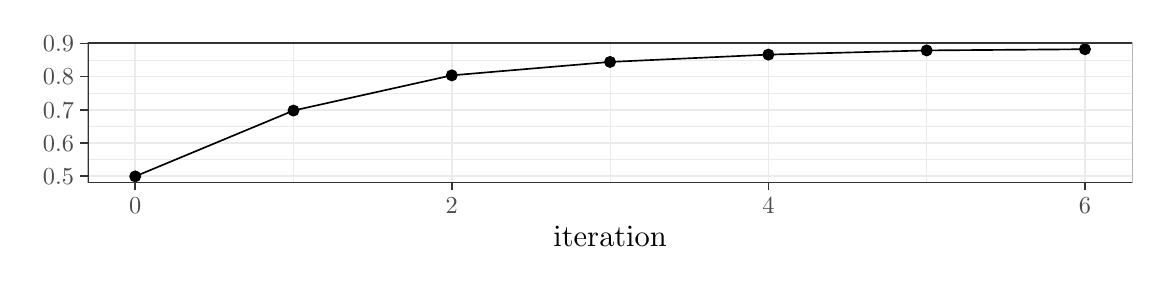
\begin{tikzpicture}[x=1pt,y=1pt]
\definecolor{fillColor}{RGB}{255,255,255}
\path[use as bounding box,fill=fillColor,fill opacity=0.00] (0,0) rectangle (404.71, 86.72);
\begin{scope}
\path[clip] (  0.00,  0.00) rectangle (404.71, 86.72);
\definecolor{drawColor}{RGB}{255,255,255}
\definecolor{fillColor}{RGB}{255,255,255}

\path[draw=drawColor,line width= 0.6pt,line join=round,line cap=round,fill=fillColor] (  0.00,  0.00) rectangle (404.71, 86.72);
\end{scope}
\begin{scope}
\path[clip] ( 21.69, 30.69) rectangle (399.21, 81.22);
\definecolor{fillColor}{RGB}{255,255,255}

\path[fill=fillColor] ( 21.69, 30.69) rectangle (399.21, 81.22);
\definecolor{drawColor}{gray}{0.92}

\path[draw=drawColor,line width= 0.3pt,line join=round] ( 21.69, 39.04) --
	(399.21, 39.04);

\path[draw=drawColor,line width= 0.3pt,line join=round] ( 21.69, 51.04) --
	(399.21, 51.04);

\path[draw=drawColor,line width= 0.3pt,line join=round] ( 21.69, 63.04) --
	(399.21, 63.04);

\path[draw=drawColor,line width= 0.3pt,line join=round] ( 21.69, 75.04) --
	(399.21, 75.04);

\path[draw=drawColor,line width= 0.3pt,line join=round] ( 96.05, 30.69) --
	( 96.05, 81.22);

\path[draw=drawColor,line width= 0.3pt,line join=round] (210.45, 30.69) --
	(210.45, 81.22);

\path[draw=drawColor,line width= 0.3pt,line join=round] (324.85, 30.69) --
	(324.85, 81.22);

\path[draw=drawColor,line width= 0.6pt,line join=round] ( 21.69, 33.04) --
	(399.21, 33.04);

\path[draw=drawColor,line width= 0.6pt,line join=round] ( 21.69, 45.04) --
	(399.21, 45.04);

\path[draw=drawColor,line width= 0.6pt,line join=round] ( 21.69, 57.04) --
	(399.21, 57.04);

\path[draw=drawColor,line width= 0.6pt,line join=round] ( 21.69, 69.04) --
	(399.21, 69.04);

\path[draw=drawColor,line width= 0.6pt,line join=round] ( 21.69, 81.04) --
	(399.21, 81.04);

\path[draw=drawColor,line width= 0.6pt,line join=round] ( 38.85, 30.69) --
	( 38.85, 81.22);

\path[draw=drawColor,line width= 0.6pt,line join=round] (153.25, 30.69) --
	(153.25, 81.22);

\path[draw=drawColor,line width= 0.6pt,line join=round] (267.65, 30.69) --
	(267.65, 81.22);

\path[draw=drawColor,line width= 0.6pt,line join=round] (382.05, 30.69) --
	(382.05, 81.22);
\definecolor{drawColor}{RGB}{0,0,0}

\path[draw=drawColor,line width= 0.6pt,line join=round] ( 38.85, 32.98) --
	( 96.05, 56.77) --
	(153.25, 69.49) --
	(210.45, 74.34) --
	(267.65, 76.98) --
	(324.85, 78.50) --
	(382.05, 78.93);
\definecolor{fillColor}{RGB}{0,0,0}

\path[draw=drawColor,line width= 0.4pt,line join=round,line cap=round,fill=fillColor] ( 38.85, 32.98) circle (  1.96);

\path[draw=drawColor,line width= 0.4pt,line join=round,line cap=round,fill=fillColor] ( 96.05, 56.77) circle (  1.96);

\path[draw=drawColor,line width= 0.4pt,line join=round,line cap=round,fill=fillColor] (153.25, 69.49) circle (  1.96);

\path[draw=drawColor,line width= 0.4pt,line join=round,line cap=round,fill=fillColor] (210.45, 74.34) circle (  1.96);

\path[draw=drawColor,line width= 0.4pt,line join=round,line cap=round,fill=fillColor] (267.65, 76.98) circle (  1.96);

\path[draw=drawColor,line width= 0.4pt,line join=round,line cap=round,fill=fillColor] (324.85, 78.50) circle (  1.96);

\path[draw=drawColor,line width= 0.4pt,line join=round,line cap=round,fill=fillColor] (382.05, 78.93) circle (  1.96);
\definecolor{drawColor}{gray}{0.20}

\path[draw=drawColor,line width= 0.6pt,line join=round,line cap=round] ( 21.69, 30.69) rectangle (399.21, 81.22);
\end{scope}
\begin{scope}
\path[clip] (  0.00,  0.00) rectangle (404.71, 86.72);
\definecolor{drawColor}{gray}{0.30}

\node[text=drawColor,anchor=base east,inner sep=0pt, outer sep=0pt, scale=  0.88] at ( 16.74, 30.01) {0.5};

\node[text=drawColor,anchor=base east,inner sep=0pt, outer sep=0pt, scale=  0.88] at ( 16.74, 42.01) {0.6};

\node[text=drawColor,anchor=base east,inner sep=0pt, outer sep=0pt, scale=  0.88] at ( 16.74, 54.01) {0.7};

\node[text=drawColor,anchor=base east,inner sep=0pt, outer sep=0pt, scale=  0.88] at ( 16.74, 66.01) {0.8};

\node[text=drawColor,anchor=base east,inner sep=0pt, outer sep=0pt, scale=  0.88] at ( 16.74, 78.01) {0.9};
\end{scope}
\begin{scope}
\path[clip] (  0.00,  0.00) rectangle (404.71, 86.72);
\definecolor{drawColor}{gray}{0.20}

\path[draw=drawColor,line width= 0.6pt,line join=round] ( 18.94, 33.04) --
	( 21.69, 33.04);

\path[draw=drawColor,line width= 0.6pt,line join=round] ( 18.94, 45.04) --
	( 21.69, 45.04);

\path[draw=drawColor,line width= 0.6pt,line join=round] ( 18.94, 57.04) --
	( 21.69, 57.04);

\path[draw=drawColor,line width= 0.6pt,line join=round] ( 18.94, 69.04) --
	( 21.69, 69.04);

\path[draw=drawColor,line width= 0.6pt,line join=round] ( 18.94, 81.04) --
	( 21.69, 81.04);
\end{scope}
\begin{scope}
\path[clip] (  0.00,  0.00) rectangle (404.71, 86.72);
\definecolor{drawColor}{gray}{0.20}

\path[draw=drawColor,line width= 0.6pt,line join=round] ( 38.85, 27.94) --
	( 38.85, 30.69);

\path[draw=drawColor,line width= 0.6pt,line join=round] (153.25, 27.94) --
	(153.25, 30.69);

\path[draw=drawColor,line width= 0.6pt,line join=round] (267.65, 27.94) --
	(267.65, 30.69);

\path[draw=drawColor,line width= 0.6pt,line join=round] (382.05, 27.94) --
	(382.05, 30.69);
\end{scope}
\begin{scope}
\path[clip] (  0.00,  0.00) rectangle (404.71, 86.72);
\definecolor{drawColor}{gray}{0.30}

\node[text=drawColor,anchor=base,inner sep=0pt, outer sep=0pt, scale=  0.88] at ( 38.85, 19.68) {0};

\node[text=drawColor,anchor=base,inner sep=0pt, outer sep=0pt, scale=  0.88] at (153.25, 19.68) {2};

\node[text=drawColor,anchor=base,inner sep=0pt, outer sep=0pt, scale=  0.88] at (267.65, 19.68) {4};

\node[text=drawColor,anchor=base,inner sep=0pt, outer sep=0pt, scale=  0.88] at (382.05, 19.68) {6};
\end{scope}
\begin{scope}
\path[clip] (  0.00,  0.00) rectangle (404.71, 86.72);
\definecolor{drawColor}{RGB}{0,0,0}

\node[text=drawColor,anchor=base,inner sep=0pt, outer sep=0pt, scale=  1.10] at (210.45,  7.64) {iteration};
\end{scope}
\end{tikzpicture}

  \caption{First six iterations for a graph with \num{500} vertices
    and average degree $16$ on the torus.  The $y$-axis of the bottom
    plot shows the fraction of monochrome edges.}
\end{figure}

\begin{figure}
  \centering
  \small
  % Created by tikzDevice version 0.12.3.1 on 2021-10-17 10:40:58
% !TEX encoding = UTF-8 Unicode
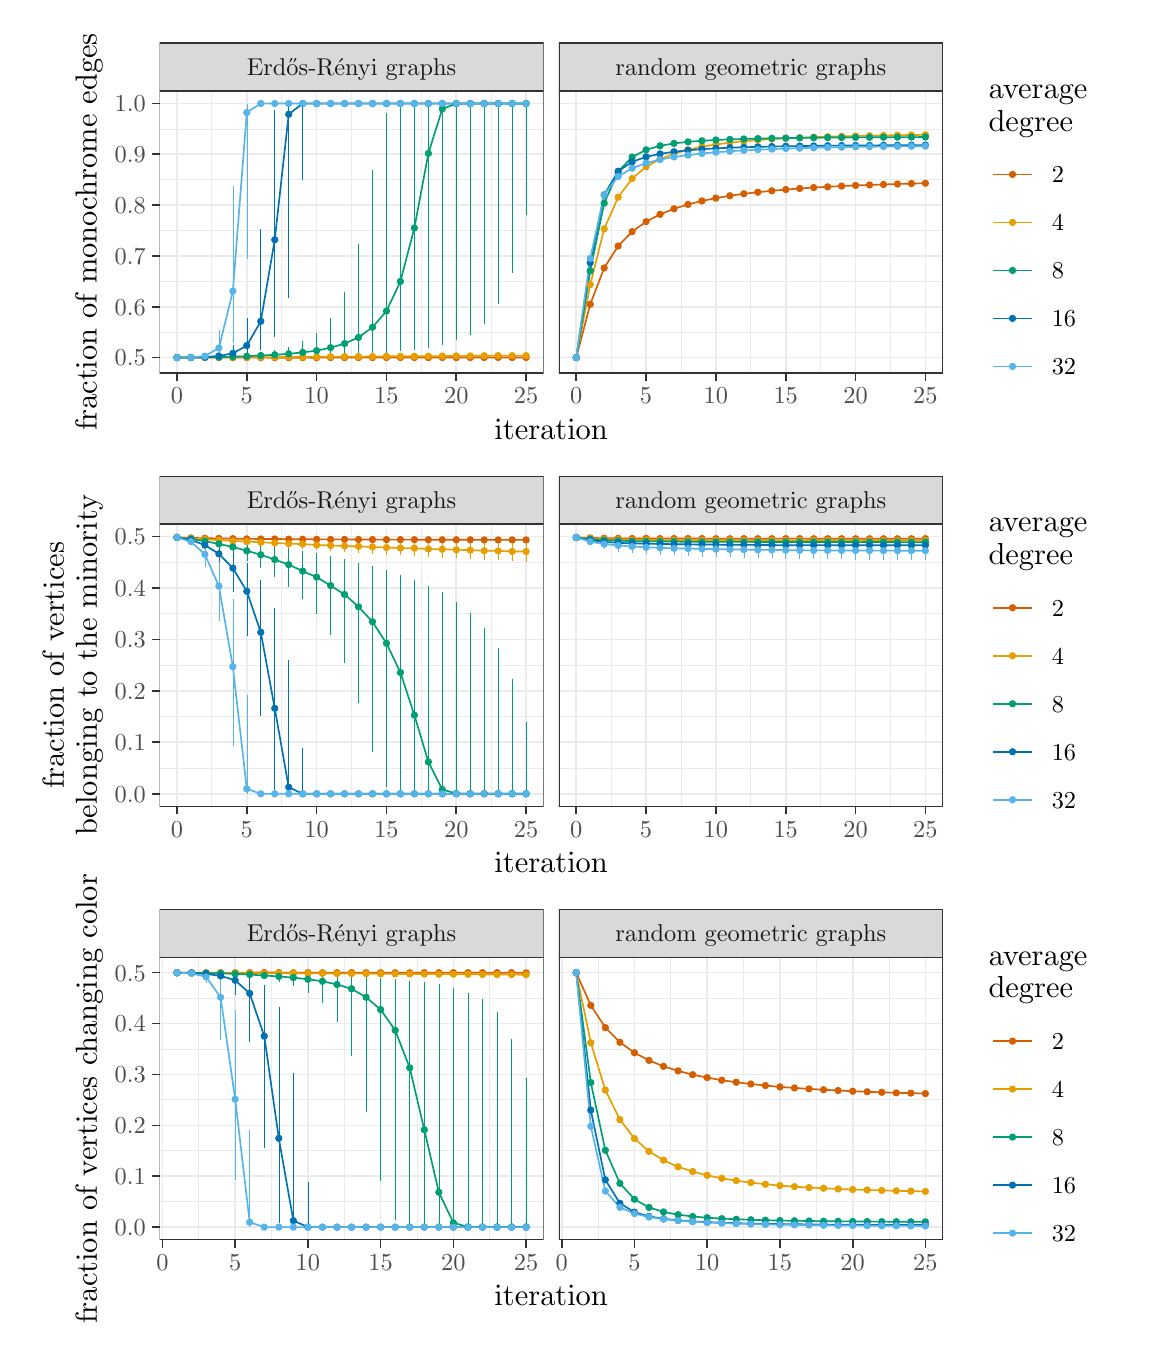
\begin{tikzpicture}[x=1pt,y=1pt]
\definecolor{fillColor}{RGB}{255,255,255}
\path[use as bounding box,fill=fillColor,fill opacity=0.00] (0,0) rectangle (397.48,469.75);
\begin{scope}
\path[clip] (  0.00,  0.00) rectangle (397.48,469.75);
\definecolor{drawColor}{gray}{0.30}

\node[text=drawColor,anchor=base east,inner sep=0pt, outer sep=0pt, scale=  0.88] at ( 42.69,347.50) {0.5};

\node[text=drawColor,anchor=base east,inner sep=0pt, outer sep=0pt, scale=  0.88] at ( 42.69,365.86) {0.6};

\node[text=drawColor,anchor=base east,inner sep=0pt, outer sep=0pt, scale=  0.88] at ( 42.69,384.22) {0.7};

\node[text=drawColor,anchor=base east,inner sep=0pt, outer sep=0pt, scale=  0.88] at ( 42.69,402.58) {0.8};

\node[text=drawColor,anchor=base east,inner sep=0pt, outer sep=0pt, scale=  0.88] at ( 42.69,420.95) {0.9};

\node[text=drawColor,anchor=base east,inner sep=0pt, outer sep=0pt, scale=  0.88] at ( 42.69,439.31) {1.0};
\end{scope}
\begin{scope}
\path[clip] (  0.00,  0.00) rectangle (397.48,469.75);
\definecolor{drawColor}{gray}{0.20}

\path[draw=drawColor,line width= 0.6pt,line join=round] ( 44.89,350.53) --
	( 47.64,350.53);

\path[draw=drawColor,line width= 0.6pt,line join=round] ( 44.89,368.89) --
	( 47.64,368.89);

\path[draw=drawColor,line width= 0.6pt,line join=round] ( 44.89,387.25) --
	( 47.64,387.25);

\path[draw=drawColor,line width= 0.6pt,line join=round] ( 44.89,405.62) --
	( 47.64,405.62);

\path[draw=drawColor,line width= 0.6pt,line join=round] ( 44.89,423.98) --
	( 47.64,423.98);

\path[draw=drawColor,line width= 0.6pt,line join=round] ( 44.89,442.34) --
	( 47.64,442.34);
\end{scope}
\begin{scope}
\path[clip] (  0.00,  0.00) rectangle (397.48,469.75);
\definecolor{drawColor}{RGB}{0,0,0}

\node[text=drawColor,rotate= 90.00,anchor=base,inner sep=0pt, outer sep=0pt, scale=  1.10] at ( 24.96,395.92) {fraction of monochrome edges};
\end{scope}
\begin{scope}
\path[clip] (  0.00,  0.00) rectangle (397.48,469.75);
\definecolor{drawColor}{gray}{0.30}

\node[text=drawColor,anchor=base east,inner sep=0pt, outer sep=0pt, scale=  0.88] at ( 42.69,189.88) {0.0};

\node[text=drawColor,anchor=base east,inner sep=0pt, outer sep=0pt, scale=  0.88] at ( 42.69,208.48) {0.1};

\node[text=drawColor,anchor=base east,inner sep=0pt, outer sep=0pt, scale=  0.88] at ( 42.69,227.09) {0.2};

\node[text=drawColor,anchor=base east,inner sep=0pt, outer sep=0pt, scale=  0.88] at ( 42.69,245.69) {0.3};

\node[text=drawColor,anchor=base east,inner sep=0pt, outer sep=0pt, scale=  0.88] at ( 42.69,264.30) {0.4};

\node[text=drawColor,anchor=base east,inner sep=0pt, outer sep=0pt, scale=  0.88] at ( 42.69,282.90) {0.5};
\end{scope}
\begin{scope}
\path[clip] (  0.00,  0.00) rectangle (397.48,469.75);
\definecolor{drawColor}{gray}{0.20}

\path[draw=drawColor,line width= 0.6pt,line join=round] ( 44.89,192.91) --
	( 47.64,192.91);

\path[draw=drawColor,line width= 0.6pt,line join=round] ( 44.89,211.51) --
	( 47.64,211.51);

\path[draw=drawColor,line width= 0.6pt,line join=round] ( 44.89,230.12) --
	( 47.64,230.12);

\path[draw=drawColor,line width= 0.6pt,line join=round] ( 44.89,248.72) --
	( 47.64,248.72);

\path[draw=drawColor,line width= 0.6pt,line join=round] ( 44.89,267.33) --
	( 47.64,267.33);

\path[draw=drawColor,line width= 0.6pt,line join=round] ( 44.89,285.93) --
	( 47.64,285.93);
\end{scope}
\begin{scope}
\path[clip] (  0.00,  0.00) rectangle (397.48,469.75);
\definecolor{drawColor}{RGB}{0,0,0}

\node[text=drawColor,rotate= 90.00,anchor=base,inner sep=0pt, outer sep=0pt, scale=  1.10] at ( 13.08,239.33) {fraction of vertices};

\node[text=drawColor,rotate= 90.00,anchor=base,inner sep=0pt, outer sep=0pt, scale=  1.10] at ( 24.96,239.33) {belonging to the minority};
\end{scope}
\begin{scope}
\path[clip] (  0.00,  0.00) rectangle (397.48,469.75);
\definecolor{drawColor}{gray}{0.30}

\node[text=drawColor,anchor=base east,inner sep=0pt, outer sep=0pt, scale=  0.88] at ( 42.69, 33.29) {0.0};

\node[text=drawColor,anchor=base east,inner sep=0pt, outer sep=0pt, scale=  0.88] at ( 42.69, 51.68) {0.1};

\node[text=drawColor,anchor=base east,inner sep=0pt, outer sep=0pt, scale=  0.88] at ( 42.69, 70.07) {0.2};

\node[text=drawColor,anchor=base east,inner sep=0pt, outer sep=0pt, scale=  0.88] at ( 42.69, 88.47) {0.3};

\node[text=drawColor,anchor=base east,inner sep=0pt, outer sep=0pt, scale=  0.88] at ( 42.69,106.86) {0.4};

\node[text=drawColor,anchor=base east,inner sep=0pt, outer sep=0pt, scale=  0.88] at ( 42.69,125.25) {0.5};
\end{scope}
\begin{scope}
\path[clip] (  0.00,  0.00) rectangle (397.48,469.75);
\definecolor{drawColor}{gray}{0.20}

\path[draw=drawColor,line width= 0.6pt,line join=round] ( 44.89, 36.32) --
	( 47.64, 36.32);

\path[draw=drawColor,line width= 0.6pt,line join=round] ( 44.89, 54.71) --
	( 47.64, 54.71);

\path[draw=drawColor,line width= 0.6pt,line join=round] ( 44.89, 73.10) --
	( 47.64, 73.10);

\path[draw=drawColor,line width= 0.6pt,line join=round] ( 44.89, 91.50) --
	( 47.64, 91.50);

\path[draw=drawColor,line width= 0.6pt,line join=round] ( 44.89,109.89) --
	( 47.64,109.89);

\path[draw=drawColor,line width= 0.6pt,line join=round] ( 44.89,128.28) --
	( 47.64,128.28);
\end{scope}
\begin{scope}
\path[clip] (  0.00,  0.00) rectangle (397.48,469.75);
\definecolor{drawColor}{RGB}{0,0,0}

\node[text=drawColor,rotate= 90.00,anchor=base,inner sep=0pt, outer sep=0pt, scale=  1.10] at ( 24.96, 82.75) {fraction of vertices changing color};
\end{scope}
\begin{scope}
\path[clip] ( 47.64,446.98) rectangle (186.42,464.26);
\definecolor{drawColor}{gray}{0.20}
\definecolor{fillColor}{gray}{0.85}

\path[draw=drawColor,line width= 0.6pt,line join=round,line cap=round,fill=fillColor] ( 47.64,446.98) rectangle (186.42,464.26);
\definecolor{drawColor}{gray}{0.10}

\node[text=drawColor,anchor=base,inner sep=0pt, outer sep=0pt, scale=  0.88] at (117.03,452.59) {Erd{\H o}s-R\'enyi graphs};
\end{scope}
\begin{scope}
\path[clip] (191.92,446.98) rectangle (330.70,464.26);
\definecolor{drawColor}{gray}{0.20}
\definecolor{fillColor}{gray}{0.85}

\path[draw=drawColor,line width= 0.6pt,line join=round,line cap=round,fill=fillColor] (191.92,446.98) rectangle (330.70,464.26);
\definecolor{drawColor}{gray}{0.10}

\node[text=drawColor,anchor=base,inner sep=0pt, outer sep=0pt, scale=  0.88] at (261.31,452.59) {random geometric graphs};
\end{scope}
\begin{scope}
\path[clip] ( 47.64,290.40) rectangle (186.42,307.67);
\definecolor{drawColor}{gray}{0.20}
\definecolor{fillColor}{gray}{0.85}

\path[draw=drawColor,line width= 0.6pt,line join=round,line cap=round,fill=fillColor] ( 47.64,290.40) rectangle (186.42,307.67);
\definecolor{drawColor}{gray}{0.10}

\node[text=drawColor,anchor=base,inner sep=0pt, outer sep=0pt, scale=  0.88] at (117.03,296.00) {Erd{\H o}s-R\'enyi graphs};
\end{scope}
\begin{scope}
\path[clip] (191.92,290.40) rectangle (330.70,307.67);
\definecolor{drawColor}{gray}{0.20}
\definecolor{fillColor}{gray}{0.85}

\path[draw=drawColor,line width= 0.6pt,line join=round,line cap=round,fill=fillColor] (191.92,290.40) rectangle (330.70,307.67);
\definecolor{drawColor}{gray}{0.10}

\node[text=drawColor,anchor=base,inner sep=0pt, outer sep=0pt, scale=  0.88] at (261.31,296.00) {random geometric graphs};
\end{scope}
\begin{scope}
\path[clip] ( 47.64,133.81) rectangle (186.42,151.09);
\definecolor{drawColor}{gray}{0.20}
\definecolor{fillColor}{gray}{0.85}

\path[draw=drawColor,line width= 0.6pt,line join=round,line cap=round,fill=fillColor] ( 47.64,133.81) rectangle (186.42,151.09);
\definecolor{drawColor}{gray}{0.10}

\node[text=drawColor,anchor=base,inner sep=0pt, outer sep=0pt, scale=  0.88] at (117.03,139.42) {Erd{\H o}s-R\'enyi graphs};
\end{scope}
\begin{scope}
\path[clip] (191.92,133.81) rectangle (330.70,151.09);
\definecolor{drawColor}{gray}{0.20}
\definecolor{fillColor}{gray}{0.85}

\path[draw=drawColor,line width= 0.6pt,line join=round,line cap=round,fill=fillColor] (191.92,133.81) rectangle (330.70,151.09);
\definecolor{drawColor}{gray}{0.10}

\node[text=drawColor,anchor=base,inner sep=0pt, outer sep=0pt, scale=  0.88] at (261.31,139.42) {random geometric graphs};
\end{scope}
\begin{scope}
\path[clip] ( 47.64,344.85) rectangle (186.42,446.98);
\definecolor{fillColor}{RGB}{255,255,255}

\path[fill=fillColor] ( 47.64,344.85) rectangle (186.42,446.98);
\definecolor{drawColor}{gray}{0.92}

\path[draw=drawColor,line width= 0.3pt,line join=round] ( 47.64,359.71) --
	(186.42,359.71);

\path[draw=drawColor,line width= 0.3pt,line join=round] ( 47.64,378.07) --
	(186.42,378.07);

\path[draw=drawColor,line width= 0.3pt,line join=round] ( 47.64,396.43) --
	(186.42,396.43);

\path[draw=drawColor,line width= 0.3pt,line join=round] ( 47.64,414.80) --
	(186.42,414.80);

\path[draw=drawColor,line width= 0.3pt,line join=round] ( 47.64,433.16) --
	(186.42,433.16);

\path[draw=drawColor,line width= 0.3pt,line join=round] ( 66.57,344.85) --
	( 66.57,446.98);

\path[draw=drawColor,line width= 0.3pt,line join=round] ( 91.80,344.85) --
	( 91.80,446.98);

\path[draw=drawColor,line width= 0.3pt,line join=round] (117.03,344.85) --
	(117.03,446.98);

\path[draw=drawColor,line width= 0.3pt,line join=round] (142.26,344.85) --
	(142.26,446.98);

\path[draw=drawColor,line width= 0.3pt,line join=round] (167.50,344.85) --
	(167.50,446.98);

\path[draw=drawColor,line width= 0.6pt,line join=round] ( 47.64,350.53) --
	(186.42,350.53);

\path[draw=drawColor,line width= 0.6pt,line join=round] ( 47.64,368.89) --
	(186.42,368.89);

\path[draw=drawColor,line width= 0.6pt,line join=round] ( 47.64,387.25) --
	(186.42,387.25);

\path[draw=drawColor,line width= 0.6pt,line join=round] ( 47.64,405.62) --
	(186.42,405.62);

\path[draw=drawColor,line width= 0.6pt,line join=round] ( 47.64,423.98) --
	(186.42,423.98);

\path[draw=drawColor,line width= 0.6pt,line join=round] ( 47.64,442.34) --
	(186.42,442.34);

\path[draw=drawColor,line width= 0.6pt,line join=round] ( 53.95,344.85) --
	( 53.95,446.98);

\path[draw=drawColor,line width= 0.6pt,line join=round] ( 79.18,344.85) --
	( 79.18,446.98);

\path[draw=drawColor,line width= 0.6pt,line join=round] (104.42,344.85) --
	(104.42,446.98);

\path[draw=drawColor,line width= 0.6pt,line join=round] (129.65,344.85) --
	(129.65,446.98);

\path[draw=drawColor,line width= 0.6pt,line join=round] (154.88,344.85) --
	(154.88,446.98);

\path[draw=drawColor,line width= 0.6pt,line join=round] (180.11,344.85) --
	(180.11,446.98);
\definecolor{drawColor}{RGB}{213,94,0}

\path[draw=drawColor,line width= 0.2pt,line join=round] ( 53.95,350.92) --
	( 53.95,350.92);

\path[draw=drawColor,line width= 0.2pt,line join=round] ( 53.95,350.92) --
	( 53.95,350.13);

\path[draw=drawColor,line width= 0.2pt,line join=round] ( 53.95,350.13) --
	( 53.95,350.13);

\path[draw=drawColor,line width= 0.2pt,line join=round] ( 59.00,351.20) --
	( 59.00,351.20);

\path[draw=drawColor,line width= 0.2pt,line join=round] ( 59.00,351.20) --
	( 59.00,349.91);

\path[draw=drawColor,line width= 0.2pt,line join=round] ( 59.00,349.91) --
	( 59.00,349.91);

\path[draw=drawColor,line width= 0.2pt,line join=round] ( 64.04,351.27) --
	( 64.04,351.27);

\path[draw=drawColor,line width= 0.2pt,line join=round] ( 64.04,351.27) --
	( 64.04,349.86);

\path[draw=drawColor,line width= 0.2pt,line join=round] ( 64.04,349.86) --
	( 64.04,349.86);

\path[draw=drawColor,line width= 0.2pt,line join=round] ( 69.09,351.30) --
	( 69.09,351.30);

\path[draw=drawColor,line width= 0.2pt,line join=round] ( 69.09,351.30) --
	( 69.09,349.82);

\path[draw=drawColor,line width= 0.2pt,line join=round] ( 69.09,349.82) --
	( 69.09,349.82);

\path[draw=drawColor,line width= 0.2pt,line join=round] ( 74.14,351.30) --
	( 74.14,351.30);

\path[draw=drawColor,line width= 0.2pt,line join=round] ( 74.14,351.30) --
	( 74.14,349.76);

\path[draw=drawColor,line width= 0.2pt,line join=round] ( 74.14,349.76) --
	( 74.14,349.76);

\path[draw=drawColor,line width= 0.2pt,line join=round] ( 79.18,351.30) --
	( 79.18,351.30);

\path[draw=drawColor,line width= 0.2pt,line join=round] ( 79.18,351.30) --
	( 79.18,349.78);

\path[draw=drawColor,line width= 0.2pt,line join=round] ( 79.18,349.78) --
	( 79.18,349.78);

\path[draw=drawColor,line width= 0.2pt,line join=round] ( 84.23,351.34) --
	( 84.23,351.34);

\path[draw=drawColor,line width= 0.2pt,line join=round] ( 84.23,351.34) --
	( 84.23,349.69);

\path[draw=drawColor,line width= 0.2pt,line join=round] ( 84.23,349.69) --
	( 84.23,349.69);

\path[draw=drawColor,line width= 0.2pt,line join=round] ( 89.28,351.34) --
	( 89.28,351.34);

\path[draw=drawColor,line width= 0.2pt,line join=round] ( 89.28,351.34) --
	( 89.28,349.65);

\path[draw=drawColor,line width= 0.2pt,line join=round] ( 89.28,349.65) --
	( 89.28,349.65);

\path[draw=drawColor,line width= 0.2pt,line join=round] ( 94.32,351.40) --
	( 94.32,351.40);

\path[draw=drawColor,line width= 0.2pt,line join=round] ( 94.32,351.40) --
	( 94.32,349.61);

\path[draw=drawColor,line width= 0.2pt,line join=round] ( 94.32,349.61) --
	( 94.32,349.61);

\path[draw=drawColor,line width= 0.2pt,line join=round] ( 99.37,351.44) --
	( 99.37,351.44);

\path[draw=drawColor,line width= 0.2pt,line join=round] ( 99.37,351.44) --
	( 99.37,349.56);

\path[draw=drawColor,line width= 0.2pt,line join=round] ( 99.37,349.56) --
	( 99.37,349.56);

\path[draw=drawColor,line width= 0.2pt,line join=round] (104.42,351.42) --
	(104.42,351.42);

\path[draw=drawColor,line width= 0.2pt,line join=round] (104.42,351.42) --
	(104.42,349.53);

\path[draw=drawColor,line width= 0.2pt,line join=round] (104.42,349.53) --
	(104.42,349.53);

\path[draw=drawColor,line width= 0.2pt,line join=round] (109.46,351.45) --
	(109.46,351.45);

\path[draw=drawColor,line width= 0.2pt,line join=round] (109.46,351.45) --
	(109.46,349.60);

\path[draw=drawColor,line width= 0.2pt,line join=round] (109.46,349.60) --
	(109.46,349.60);

\path[draw=drawColor,line width= 0.2pt,line join=round] (114.51,351.48) --
	(114.51,351.48);

\path[draw=drawColor,line width= 0.2pt,line join=round] (114.51,351.48) --
	(114.51,349.55);

\path[draw=drawColor,line width= 0.2pt,line join=round] (114.51,349.55) --
	(114.51,349.55);

\path[draw=drawColor,line width= 0.2pt,line join=round] (119.55,351.49) --
	(119.55,351.49);

\path[draw=drawColor,line width= 0.2pt,line join=round] (119.55,351.49) --
	(119.55,349.61);

\path[draw=drawColor,line width= 0.2pt,line join=round] (119.55,349.61) --
	(119.55,349.61);

\path[draw=drawColor,line width= 0.2pt,line join=round] (124.60,351.52) --
	(124.60,351.52);

\path[draw=drawColor,line width= 0.2pt,line join=round] (124.60,351.52) --
	(124.60,349.58);

\path[draw=drawColor,line width= 0.2pt,line join=round] (124.60,349.58) --
	(124.60,349.58);

\path[draw=drawColor,line width= 0.2pt,line join=round] (129.65,351.55) --
	(129.65,351.55);

\path[draw=drawColor,line width= 0.2pt,line join=round] (129.65,351.55) --
	(129.65,349.56);

\path[draw=drawColor,line width= 0.2pt,line join=round] (129.65,349.56) --
	(129.65,349.56);

\path[draw=drawColor,line width= 0.2pt,line join=round] (134.69,351.55) --
	(134.69,351.55);

\path[draw=drawColor,line width= 0.2pt,line join=round] (134.69,351.55) --
	(134.69,349.56);

\path[draw=drawColor,line width= 0.2pt,line join=round] (134.69,349.56) --
	(134.69,349.56);

\path[draw=drawColor,line width= 0.2pt,line join=round] (139.74,351.54) --
	(139.74,351.54);

\path[draw=drawColor,line width= 0.2pt,line join=round] (139.74,351.54) --
	(139.74,349.58);

\path[draw=drawColor,line width= 0.2pt,line join=round] (139.74,349.58) --
	(139.74,349.58);

\path[draw=drawColor,line width= 0.2pt,line join=round] (144.79,351.58) --
	(144.79,351.58);

\path[draw=drawColor,line width= 0.2pt,line join=round] (144.79,351.58) --
	(144.79,349.53);

\path[draw=drawColor,line width= 0.2pt,line join=round] (144.79,349.53) --
	(144.79,349.53);

\path[draw=drawColor,line width= 0.2pt,line join=round] (149.83,351.55) --
	(149.83,351.55);

\path[draw=drawColor,line width= 0.2pt,line join=round] (149.83,351.55) --
	(149.83,349.57);

\path[draw=drawColor,line width= 0.2pt,line join=round] (149.83,349.57) --
	(149.83,349.57);

\path[draw=drawColor,line width= 0.2pt,line join=round] (154.88,351.56) --
	(154.88,351.56);

\path[draw=drawColor,line width= 0.2pt,line join=round] (154.88,351.56) --
	(154.88,349.57);

\path[draw=drawColor,line width= 0.2pt,line join=round] (154.88,349.57) --
	(154.88,349.57);

\path[draw=drawColor,line width= 0.2pt,line join=round] (159.93,351.59) --
	(159.93,351.59);

\path[draw=drawColor,line width= 0.2pt,line join=round] (159.93,351.59) --
	(159.93,349.52);

\path[draw=drawColor,line width= 0.2pt,line join=round] (159.93,349.52) --
	(159.93,349.52);

\path[draw=drawColor,line width= 0.2pt,line join=round] (164.97,351.59) --
	(164.97,351.59);

\path[draw=drawColor,line width= 0.2pt,line join=round] (164.97,351.59) --
	(164.97,349.55);

\path[draw=drawColor,line width= 0.2pt,line join=round] (164.97,349.55) --
	(164.97,349.55);

\path[draw=drawColor,line width= 0.2pt,line join=round] (170.02,351.55) --
	(170.02,351.55);

\path[draw=drawColor,line width= 0.2pt,line join=round] (170.02,351.55) --
	(170.02,349.52);

\path[draw=drawColor,line width= 0.2pt,line join=round] (170.02,349.52) --
	(170.02,349.52);

\path[draw=drawColor,line width= 0.2pt,line join=round] (175.07,351.60) --
	(175.07,351.60);

\path[draw=drawColor,line width= 0.2pt,line join=round] (175.07,351.60) --
	(175.07,349.56);

\path[draw=drawColor,line width= 0.2pt,line join=round] (175.07,349.56) --
	(175.07,349.56);

\path[draw=drawColor,line width= 0.2pt,line join=round] (180.11,351.55) --
	(180.11,351.55);

\path[draw=drawColor,line width= 0.2pt,line join=round] (180.11,351.55) --
	(180.11,349.49);

\path[draw=drawColor,line width= 0.2pt,line join=round] (180.11,349.49) --
	(180.11,349.49);
\definecolor{drawColor}{RGB}{230,159,0}

\path[draw=drawColor,line width= 0.2pt,line join=round] ( 53.95,350.83) --
	( 53.95,350.83);

\path[draw=drawColor,line width= 0.2pt,line join=round] ( 53.95,350.83) --
	( 53.95,350.30);

\path[draw=drawColor,line width= 0.2pt,line join=round] ( 53.95,350.30) --
	( 53.95,350.30);

\path[draw=drawColor,line width= 0.2pt,line join=round] ( 59.00,351.02) --
	( 59.00,351.02);

\path[draw=drawColor,line width= 0.2pt,line join=round] ( 59.00,351.02) --
	( 59.00,350.13);

\path[draw=drawColor,line width= 0.2pt,line join=round] ( 59.00,350.13) --
	( 59.00,350.13);

\path[draw=drawColor,line width= 0.2pt,line join=round] ( 64.04,351.13) --
	( 64.04,351.13);

\path[draw=drawColor,line width= 0.2pt,line join=round] ( 64.04,351.13) --
	( 64.04,350.06);

\path[draw=drawColor,line width= 0.2pt,line join=round] ( 64.04,350.06) --
	( 64.04,350.06);

\path[draw=drawColor,line width= 0.2pt,line join=round] ( 69.09,351.24) --
	( 69.09,351.24);

\path[draw=drawColor,line width= 0.2pt,line join=round] ( 69.09,351.24) --
	( 69.09,350.00);

\path[draw=drawColor,line width= 0.2pt,line join=round] ( 69.09,350.00) --
	( 69.09,350.00);

\path[draw=drawColor,line width= 0.2pt,line join=round] ( 74.14,351.33) --
	( 74.14,351.33);

\path[draw=drawColor,line width= 0.2pt,line join=round] ( 74.14,351.33) --
	( 74.14,349.95);

\path[draw=drawColor,line width= 0.2pt,line join=round] ( 74.14,349.95) --
	( 74.14,349.95);

\path[draw=drawColor,line width= 0.2pt,line join=round] ( 79.18,351.37) --
	( 79.18,351.37);

\path[draw=drawColor,line width= 0.2pt,line join=round] ( 79.18,351.37) --
	( 79.18,349.93);

\path[draw=drawColor,line width= 0.2pt,line join=round] ( 79.18,349.93) --
	( 79.18,349.93);

\path[draw=drawColor,line width= 0.2pt,line join=round] ( 84.23,351.44) --
	( 84.23,351.44);

\path[draw=drawColor,line width= 0.2pt,line join=round] ( 84.23,351.44) --
	( 84.23,349.91);

\path[draw=drawColor,line width= 0.2pt,line join=round] ( 84.23,349.91) --
	( 84.23,349.91);

\path[draw=drawColor,line width= 0.2pt,line join=round] ( 89.28,351.44) --
	( 89.28,351.44);

\path[draw=drawColor,line width= 0.2pt,line join=round] ( 89.28,351.44) --
	( 89.28,349.92);

\path[draw=drawColor,line width= 0.2pt,line join=round] ( 89.28,349.92) --
	( 89.28,349.92);

\path[draw=drawColor,line width= 0.2pt,line join=round] ( 94.32,351.49) --
	( 94.32,351.49);

\path[draw=drawColor,line width= 0.2pt,line join=round] ( 94.32,351.49) --
	( 94.32,349.94);

\path[draw=drawColor,line width= 0.2pt,line join=round] ( 94.32,349.94) --
	( 94.32,349.94);

\path[draw=drawColor,line width= 0.2pt,line join=round] ( 99.37,351.55) --
	( 99.37,351.55);

\path[draw=drawColor,line width= 0.2pt,line join=round] ( 99.37,351.55) --
	( 99.37,349.97);

\path[draw=drawColor,line width= 0.2pt,line join=round] ( 99.37,349.97) --
	( 99.37,349.97);

\path[draw=drawColor,line width= 0.2pt,line join=round] (104.42,351.64) --
	(104.42,351.64);

\path[draw=drawColor,line width= 0.2pt,line join=round] (104.42,351.64) --
	(104.42,349.93);

\path[draw=drawColor,line width= 0.2pt,line join=round] (104.42,349.93) --
	(104.42,349.93);

\path[draw=drawColor,line width= 0.2pt,line join=round] (109.46,351.75) --
	(109.46,351.75);

\path[draw=drawColor,line width= 0.2pt,line join=round] (109.46,351.75) --
	(109.46,349.98);

\path[draw=drawColor,line width= 0.2pt,line join=round] (109.46,349.98) --
	(109.46,349.98);

\path[draw=drawColor,line width= 0.2pt,line join=round] (114.51,351.77) --
	(114.51,351.77);

\path[draw=drawColor,line width= 0.2pt,line join=round] (114.51,351.77) --
	(114.51,349.98);

\path[draw=drawColor,line width= 0.2pt,line join=round] (114.51,349.98) --
	(114.51,349.98);

\path[draw=drawColor,line width= 0.2pt,line join=round] (119.55,351.76) --
	(119.55,351.76);

\path[draw=drawColor,line width= 0.2pt,line join=round] (119.55,351.76) --
	(119.55,350.03);

\path[draw=drawColor,line width= 0.2pt,line join=round] (119.55,350.03) --
	(119.55,350.03);

\path[draw=drawColor,line width= 0.2pt,line join=round] (124.60,351.83) --
	(124.60,351.83);

\path[draw=drawColor,line width= 0.2pt,line join=round] (124.60,351.83) --
	(124.60,349.97);

\path[draw=drawColor,line width= 0.2pt,line join=round] (124.60,349.97) --
	(124.60,349.97);

\path[draw=drawColor,line width= 0.2pt,line join=round] (129.65,351.92) --
	(129.65,351.92);

\path[draw=drawColor,line width= 0.2pt,line join=round] (129.65,351.92) --
	(129.65,350.05);

\path[draw=drawColor,line width= 0.2pt,line join=round] (129.65,350.05) --
	(129.65,350.05);

\path[draw=drawColor,line width= 0.2pt,line join=round] (134.69,351.93) --
	(134.69,351.93);

\path[draw=drawColor,line width= 0.2pt,line join=round] (134.69,351.93) --
	(134.69,350.01);

\path[draw=drawColor,line width= 0.2pt,line join=round] (134.69,350.01) --
	(134.69,350.01);

\path[draw=drawColor,line width= 0.2pt,line join=round] (139.74,351.94) --
	(139.74,351.94);

\path[draw=drawColor,line width= 0.2pt,line join=round] (139.74,351.94) --
	(139.74,350.10);

\path[draw=drawColor,line width= 0.2pt,line join=round] (139.74,350.10) --
	(139.74,350.10);

\path[draw=drawColor,line width= 0.2pt,line join=round] (144.79,352.09) --
	(144.79,352.09);

\path[draw=drawColor,line width= 0.2pt,line join=round] (144.79,352.09) --
	(144.79,350.08);

\path[draw=drawColor,line width= 0.2pt,line join=round] (144.79,350.08) --
	(144.79,350.08);

\path[draw=drawColor,line width= 0.2pt,line join=round] (149.83,352.13) --
	(149.83,352.13);

\path[draw=drawColor,line width= 0.2pt,line join=round] (149.83,352.13) --
	(149.83,350.14);

\path[draw=drawColor,line width= 0.2pt,line join=round] (149.83,350.14) --
	(149.83,350.14);

\path[draw=drawColor,line width= 0.2pt,line join=round] (154.88,352.14) --
	(154.88,352.14);

\path[draw=drawColor,line width= 0.2pt,line join=round] (154.88,352.14) --
	(154.88,350.05);

\path[draw=drawColor,line width= 0.2pt,line join=round] (154.88,350.05) --
	(154.88,350.05);

\path[draw=drawColor,line width= 0.2pt,line join=round] (159.93,352.17) --
	(159.93,352.17);

\path[draw=drawColor,line width= 0.2pt,line join=round] (159.93,352.17) --
	(159.93,350.13);

\path[draw=drawColor,line width= 0.2pt,line join=round] (159.93,350.13) --
	(159.93,350.13);

\path[draw=drawColor,line width= 0.2pt,line join=round] (164.97,352.23) --
	(164.97,352.23);

\path[draw=drawColor,line width= 0.2pt,line join=round] (164.97,352.23) --
	(164.97,350.14);

\path[draw=drawColor,line width= 0.2pt,line join=round] (164.97,350.14) --
	(164.97,350.14);

\path[draw=drawColor,line width= 0.2pt,line join=round] (170.02,352.31) --
	(170.02,352.31);

\path[draw=drawColor,line width= 0.2pt,line join=round] (170.02,352.31) --
	(170.02,350.18);

\path[draw=drawColor,line width= 0.2pt,line join=round] (170.02,350.18) --
	(170.02,350.18);

\path[draw=drawColor,line width= 0.2pt,line join=round] (175.07,352.37) --
	(175.07,352.37);

\path[draw=drawColor,line width= 0.2pt,line join=round] (175.07,352.37) --
	(175.07,350.16);

\path[draw=drawColor,line width= 0.2pt,line join=round] (175.07,350.16) --
	(175.07,350.16);

\path[draw=drawColor,line width= 0.2pt,line join=round] (180.11,352.37) --
	(180.11,352.37);

\path[draw=drawColor,line width= 0.2pt,line join=round] (180.11,352.37) --
	(180.11,350.22);

\path[draw=drawColor,line width= 0.2pt,line join=round] (180.11,350.22) --
	(180.11,350.22);
\definecolor{drawColor}{RGB}{0,158,115}

\path[draw=drawColor,line width= 0.2pt,line join=round] ( 53.95,350.73) --
	( 53.95,350.73);

\path[draw=drawColor,line width= 0.2pt,line join=round] ( 53.95,350.73) --
	( 53.95,350.33);

\path[draw=drawColor,line width= 0.2pt,line join=round] ( 53.95,350.33) --
	( 53.95,350.33);

\path[draw=drawColor,line width= 0.2pt,line join=round] ( 59.00,350.87) --
	( 59.00,350.87);

\path[draw=drawColor,line width= 0.2pt,line join=round] ( 59.00,350.87) --
	( 59.00,350.22);

\path[draw=drawColor,line width= 0.2pt,line join=round] ( 59.00,350.22) --
	( 59.00,350.22);

\path[draw=drawColor,line width= 0.2pt,line join=round] ( 64.04,351.00) --
	( 64.04,351.00);

\path[draw=drawColor,line width= 0.2pt,line join=round] ( 64.04,351.00) --
	( 64.04,350.23);

\path[draw=drawColor,line width= 0.2pt,line join=round] ( 64.04,350.23) --
	( 64.04,350.23);

\path[draw=drawColor,line width= 0.2pt,line join=round] ( 69.09,351.22) --
	( 69.09,351.22);

\path[draw=drawColor,line width= 0.2pt,line join=round] ( 69.09,351.22) --
	( 69.09,350.23);

\path[draw=drawColor,line width= 0.2pt,line join=round] ( 69.09,350.23) --
	( 69.09,350.23);

\path[draw=drawColor,line width= 0.2pt,line join=round] ( 74.14,351.45) --
	( 74.14,351.45);

\path[draw=drawColor,line width= 0.2pt,line join=round] ( 74.14,351.45) --
	( 74.14,350.32);

\path[draw=drawColor,line width= 0.2pt,line join=round] ( 74.14,350.32) --
	( 74.14,350.32);

\path[draw=drawColor,line width= 0.2pt,line join=round] ( 79.18,351.77) --
	( 79.18,351.77);

\path[draw=drawColor,line width= 0.2pt,line join=round] ( 79.18,351.77) --
	( 79.18,350.40);

\path[draw=drawColor,line width= 0.2pt,line join=round] ( 79.18,350.40) --
	( 79.18,350.40);

\path[draw=drawColor,line width= 0.2pt,line join=round] ( 84.23,352.27) --
	( 84.23,352.27);

\path[draw=drawColor,line width= 0.2pt,line join=round] ( 84.23,352.27) --
	( 84.23,350.51);

\path[draw=drawColor,line width= 0.2pt,line join=round] ( 84.23,350.51) --
	( 84.23,350.51);

\path[draw=drawColor,line width= 0.2pt,line join=round] ( 89.28,353.13) --
	( 89.28,353.13);

\path[draw=drawColor,line width= 0.2pt,line join=round] ( 89.28,353.13) --
	( 89.28,350.64);

\path[draw=drawColor,line width= 0.2pt,line join=round] ( 89.28,350.64) --
	( 89.28,350.64);

\path[draw=drawColor,line width= 0.2pt,line join=round] ( 94.32,354.49) --
	( 94.32,354.49);

\path[draw=drawColor,line width= 0.2pt,line join=round] ( 94.32,354.49) --
	( 94.32,350.76);

\path[draw=drawColor,line width= 0.2pt,line join=round] ( 94.32,350.76) --
	( 94.32,350.76);

\path[draw=drawColor,line width= 0.2pt,line join=round] ( 99.37,356.43) --
	( 99.37,356.43);

\path[draw=drawColor,line width= 0.2pt,line join=round] ( 99.37,356.43) --
	( 99.37,350.92);

\path[draw=drawColor,line width= 0.2pt,line join=round] ( 99.37,350.92) --
	( 99.37,350.92);

\path[draw=drawColor,line width= 0.2pt,line join=round] (104.42,359.58) --
	(104.42,359.58);

\path[draw=drawColor,line width= 0.2pt,line join=round] (104.42,359.58) --
	(104.42,351.12);

\path[draw=drawColor,line width= 0.2pt,line join=round] (104.42,351.12) --
	(104.42,351.12);

\path[draw=drawColor,line width= 0.2pt,line join=round] (109.46,364.77) --
	(109.46,364.77);

\path[draw=drawColor,line width= 0.2pt,line join=round] (109.46,364.77) --
	(109.46,351.31);

\path[draw=drawColor,line width= 0.2pt,line join=round] (109.46,351.31) --
	(109.46,351.31);

\path[draw=drawColor,line width= 0.2pt,line join=round] (114.51,374.38) --
	(114.51,374.38);

\path[draw=drawColor,line width= 0.2pt,line join=round] (114.51,374.38) --
	(114.51,351.56);

\path[draw=drawColor,line width= 0.2pt,line join=round] (114.51,351.56) --
	(114.51,351.56);

\path[draw=drawColor,line width= 0.2pt,line join=round] (119.55,391.42) --
	(119.55,391.42);

\path[draw=drawColor,line width= 0.2pt,line join=round] (119.55,391.42) --
	(119.55,351.71);

\path[draw=drawColor,line width= 0.2pt,line join=round] (119.55,351.71) --
	(119.55,351.71);

\path[draw=drawColor,line width= 0.2pt,line join=round] (124.60,418.22) --
	(124.60,418.22);

\path[draw=drawColor,line width= 0.2pt,line join=round] (124.60,418.22) --
	(124.60,352.07);

\path[draw=drawColor,line width= 0.2pt,line join=round] (124.60,352.07) --
	(124.60,352.07);

\path[draw=drawColor,line width= 0.2pt,line join=round] (129.65,438.96) --
	(129.65,438.96);

\path[draw=drawColor,line width= 0.2pt,line join=round] (129.65,438.96) --
	(129.65,352.36);

\path[draw=drawColor,line width= 0.2pt,line join=round] (129.65,352.36) --
	(129.65,352.36);

\path[draw=drawColor,line width= 0.2pt,line join=round] (134.69,442.25) --
	(134.69,442.25);

\path[draw=drawColor,line width= 0.2pt,line join=round] (134.69,442.25) --
	(134.69,352.75);

\path[draw=drawColor,line width= 0.2pt,line join=round] (134.69,352.75) --
	(134.69,352.75);

\path[draw=drawColor,line width= 0.2pt,line join=round] (139.74,442.34) --
	(139.74,442.34);

\path[draw=drawColor,line width= 0.2pt,line join=round] (139.74,442.34) --
	(139.74,353.37);

\path[draw=drawColor,line width= 0.2pt,line join=round] (139.74,353.37) --
	(139.74,353.37);

\path[draw=drawColor,line width= 0.2pt,line join=round] (144.79,442.34) --
	(144.79,442.34);

\path[draw=drawColor,line width= 0.2pt,line join=round] (144.79,442.34) --
	(144.79,354.11);

\path[draw=drawColor,line width= 0.2pt,line join=round] (144.79,354.11) --
	(144.79,354.11);

\path[draw=drawColor,line width= 0.2pt,line join=round] (149.83,442.34) --
	(149.83,442.34);

\path[draw=drawColor,line width= 0.2pt,line join=round] (149.83,442.34) --
	(149.83,355.02);

\path[draw=drawColor,line width= 0.2pt,line join=round] (149.83,355.02) --
	(149.83,355.02);

\path[draw=drawColor,line width= 0.2pt,line join=round] (154.88,442.34) --
	(154.88,442.34);

\path[draw=drawColor,line width= 0.2pt,line join=round] (154.88,442.34) --
	(154.88,356.73);

\path[draw=drawColor,line width= 0.2pt,line join=round] (154.88,356.73) --
	(154.88,356.73);

\path[draw=drawColor,line width= 0.2pt,line join=round] (159.93,442.34) --
	(159.93,442.34);

\path[draw=drawColor,line width= 0.2pt,line join=round] (159.93,442.34) --
	(159.93,358.54);

\path[draw=drawColor,line width= 0.2pt,line join=round] (159.93,358.54) --
	(159.93,358.54);

\path[draw=drawColor,line width= 0.2pt,line join=round] (164.97,442.34) --
	(164.97,442.34);

\path[draw=drawColor,line width= 0.2pt,line join=round] (164.97,442.34) --
	(164.97,362.74);

\path[draw=drawColor,line width= 0.2pt,line join=round] (164.97,362.74) --
	(164.97,362.74);

\path[draw=drawColor,line width= 0.2pt,line join=round] (170.02,442.34) --
	(170.02,442.34);

\path[draw=drawColor,line width= 0.2pt,line join=round] (170.02,442.34) --
	(170.02,369.94);

\path[draw=drawColor,line width= 0.2pt,line join=round] (170.02,369.94) --
	(170.02,369.94);

\path[draw=drawColor,line width= 0.2pt,line join=round] (175.07,442.34) --
	(175.07,442.34);

\path[draw=drawColor,line width= 0.2pt,line join=round] (175.07,442.34) --
	(175.07,381.24);

\path[draw=drawColor,line width= 0.2pt,line join=round] (175.07,381.24) --
	(175.07,381.24);

\path[draw=drawColor,line width= 0.2pt,line join=round] (180.11,442.34) --
	(180.11,442.34);

\path[draw=drawColor,line width= 0.2pt,line join=round] (180.11,442.34) --
	(180.11,401.91);

\path[draw=drawColor,line width= 0.2pt,line join=round] (180.11,401.91) --
	(180.11,401.91);
\definecolor{drawColor}{RGB}{0,114,178}

\path[draw=drawColor,line width= 0.2pt,line join=round] ( 53.95,350.66) --
	( 53.95,350.66);

\path[draw=drawColor,line width= 0.2pt,line join=round] ( 53.95,350.66) --
	( 53.95,350.39);

\path[draw=drawColor,line width= 0.2pt,line join=round] ( 53.95,350.39) --
	( 53.95,350.39);

\path[draw=drawColor,line width= 0.2pt,line join=round] ( 59.00,350.81) --
	( 59.00,350.81);

\path[draw=drawColor,line width= 0.2pt,line join=round] ( 59.00,350.81) --
	( 59.00,350.33);

\path[draw=drawColor,line width= 0.2pt,line join=round] ( 59.00,350.33) --
	( 59.00,350.33);

\path[draw=drawColor,line width= 0.2pt,line join=round] ( 64.04,351.08) --
	( 64.04,351.08);

\path[draw=drawColor,line width= 0.2pt,line join=round] ( 64.04,351.08) --
	( 64.04,350.41);

\path[draw=drawColor,line width= 0.2pt,line join=round] ( 64.04,350.41) --
	( 64.04,350.41);

\path[draw=drawColor,line width= 0.2pt,line join=round] ( 69.09,351.96) --
	( 69.09,351.96);

\path[draw=drawColor,line width= 0.2pt,line join=round] ( 69.09,351.96) --
	( 69.09,350.61);

\path[draw=drawColor,line width= 0.2pt,line join=round] ( 69.09,350.61) --
	( 69.09,350.61);

\path[draw=drawColor,line width= 0.2pt,line join=round] ( 74.14,355.03) --
	( 74.14,355.03);

\path[draw=drawColor,line width= 0.2pt,line join=round] ( 74.14,355.03) --
	( 74.14,350.95);

\path[draw=drawColor,line width= 0.2pt,line join=round] ( 74.14,350.95) --
	( 74.14,350.95);

\path[draw=drawColor,line width= 0.2pt,line join=round] ( 79.18,364.77) --
	( 79.18,364.77);

\path[draw=drawColor,line width= 0.2pt,line join=round] ( 79.18,364.77) --
	( 79.18,351.56);

\path[draw=drawColor,line width= 0.2pt,line join=round] ( 79.18,351.56) --
	( 79.18,351.56);

\path[draw=drawColor,line width= 0.2pt,line join=round] ( 84.23,396.95) --
	( 84.23,396.95);

\path[draw=drawColor,line width= 0.2pt,line join=round] ( 84.23,396.95) --
	( 84.23,353.12);

\path[draw=drawColor,line width= 0.2pt,line join=round] ( 84.23,353.12) --
	( 84.23,353.12);

\path[draw=drawColor,line width= 0.2pt,line join=round] ( 89.28,440.06) --
	( 89.28,440.06);

\path[draw=drawColor,line width= 0.2pt,line join=round] ( 89.28,440.06) --
	( 89.28,357.84);

\path[draw=drawColor,line width= 0.2pt,line join=round] ( 89.28,357.84) --
	( 89.28,357.84);

\path[draw=drawColor,line width= 0.2pt,line join=round] ( 94.32,442.34) --
	( 94.32,442.34);

\path[draw=drawColor,line width= 0.2pt,line join=round] ( 94.32,442.34) --
	( 94.32,372.14);

\path[draw=drawColor,line width= 0.2pt,line join=round] ( 94.32,372.14) --
	( 94.32,372.14);

\path[draw=drawColor,line width= 0.2pt,line join=round] ( 99.37,442.34) --
	( 99.37,442.34);

\path[draw=drawColor,line width= 0.2pt,line join=round] ( 99.37,442.34) --
	( 99.37,414.56);

\path[draw=drawColor,line width= 0.2pt,line join=round] ( 99.37,414.56) --
	( 99.37,414.56);

\path[draw=drawColor,line width= 0.2pt,line join=round] (104.42,442.34) --
	(104.42,442.34);

\path[draw=drawColor,line width= 0.2pt,line join=round] (104.42,442.34) --
	(104.42,442.15);

\path[draw=drawColor,line width= 0.2pt,line join=round] (104.42,442.15) --
	(104.42,442.15);

\path[draw=drawColor,line width= 0.2pt,line join=round] (109.46,442.34) --
	(109.46,442.34);

\path[draw=drawColor,line width= 0.2pt,line join=round] (109.46,442.34) --
	(109.46,442.34);

\path[draw=drawColor,line width= 0.2pt,line join=round] (109.46,442.34) --
	(109.46,442.34);

\path[draw=drawColor,line width= 0.2pt,line join=round] (114.51,442.34) --
	(114.51,442.34);

\path[draw=drawColor,line width= 0.2pt,line join=round] (114.51,442.34) --
	(114.51,442.34);

\path[draw=drawColor,line width= 0.2pt,line join=round] (114.51,442.34) --
	(114.51,442.34);

\path[draw=drawColor,line width= 0.2pt,line join=round] (119.55,442.34) --
	(119.55,442.34);

\path[draw=drawColor,line width= 0.2pt,line join=round] (119.55,442.34) --
	(119.55,442.34);

\path[draw=drawColor,line width= 0.2pt,line join=round] (119.55,442.34) --
	(119.55,442.34);

\path[draw=drawColor,line width= 0.2pt,line join=round] (124.60,442.34) --
	(124.60,442.34);

\path[draw=drawColor,line width= 0.2pt,line join=round] (124.60,442.34) --
	(124.60,442.34);

\path[draw=drawColor,line width= 0.2pt,line join=round] (124.60,442.34) --
	(124.60,442.34);

\path[draw=drawColor,line width= 0.2pt,line join=round] (129.65,442.34) --
	(129.65,442.34);

\path[draw=drawColor,line width= 0.2pt,line join=round] (129.65,442.34) --
	(129.65,442.34);

\path[draw=drawColor,line width= 0.2pt,line join=round] (129.65,442.34) --
	(129.65,442.34);

\path[draw=drawColor,line width= 0.2pt,line join=round] (134.69,442.34) --
	(134.69,442.34);

\path[draw=drawColor,line width= 0.2pt,line join=round] (134.69,442.34) --
	(134.69,442.34);

\path[draw=drawColor,line width= 0.2pt,line join=round] (134.69,442.34) --
	(134.69,442.34);

\path[draw=drawColor,line width= 0.2pt,line join=round] (139.74,442.34) --
	(139.74,442.34);

\path[draw=drawColor,line width= 0.2pt,line join=round] (139.74,442.34) --
	(139.74,442.34);

\path[draw=drawColor,line width= 0.2pt,line join=round] (139.74,442.34) --
	(139.74,442.34);

\path[draw=drawColor,line width= 0.2pt,line join=round] (144.79,442.34) --
	(144.79,442.34);

\path[draw=drawColor,line width= 0.2pt,line join=round] (144.79,442.34) --
	(144.79,442.34);

\path[draw=drawColor,line width= 0.2pt,line join=round] (144.79,442.34) --
	(144.79,442.34);

\path[draw=drawColor,line width= 0.2pt,line join=round] (149.83,442.34) --
	(149.83,442.34);

\path[draw=drawColor,line width= 0.2pt,line join=round] (149.83,442.34) --
	(149.83,442.34);

\path[draw=drawColor,line width= 0.2pt,line join=round] (149.83,442.34) --
	(149.83,442.34);

\path[draw=drawColor,line width= 0.2pt,line join=round] (154.88,442.34) --
	(154.88,442.34);

\path[draw=drawColor,line width= 0.2pt,line join=round] (154.88,442.34) --
	(154.88,442.34);

\path[draw=drawColor,line width= 0.2pt,line join=round] (154.88,442.34) --
	(154.88,442.34);

\path[draw=drawColor,line width= 0.2pt,line join=round] (159.93,442.34) --
	(159.93,442.34);

\path[draw=drawColor,line width= 0.2pt,line join=round] (159.93,442.34) --
	(159.93,442.34);

\path[draw=drawColor,line width= 0.2pt,line join=round] (159.93,442.34) --
	(159.93,442.34);

\path[draw=drawColor,line width= 0.2pt,line join=round] (164.97,442.34) --
	(164.97,442.34);

\path[draw=drawColor,line width= 0.2pt,line join=round] (164.97,442.34) --
	(164.97,442.34);

\path[draw=drawColor,line width= 0.2pt,line join=round] (164.97,442.34) --
	(164.97,442.34);

\path[draw=drawColor,line width= 0.2pt,line join=round] (170.02,442.34) --
	(170.02,442.34);

\path[draw=drawColor,line width= 0.2pt,line join=round] (170.02,442.34) --
	(170.02,442.34);

\path[draw=drawColor,line width= 0.2pt,line join=round] (170.02,442.34) --
	(170.02,442.34);

\path[draw=drawColor,line width= 0.2pt,line join=round] (175.07,442.34) --
	(175.07,442.34);

\path[draw=drawColor,line width= 0.2pt,line join=round] (175.07,442.34) --
	(175.07,442.34);

\path[draw=drawColor,line width= 0.2pt,line join=round] (175.07,442.34) --
	(175.07,442.34);

\path[draw=drawColor,line width= 0.2pt,line join=round] (180.11,442.34) --
	(180.11,442.34);

\path[draw=drawColor,line width= 0.2pt,line join=round] (180.11,442.34) --
	(180.11,442.34);

\path[draw=drawColor,line width= 0.2pt,line join=round] (180.11,442.34) --
	(180.11,442.34);
\definecolor{drawColor}{RGB}{86,180,233}

\path[draw=drawColor,line width= 0.2pt,line join=round] ( 53.95,350.63) --
	( 53.95,350.63);

\path[draw=drawColor,line width= 0.2pt,line join=round] ( 53.95,350.63) --
	( 53.95,350.42);

\path[draw=drawColor,line width= 0.2pt,line join=round] ( 53.95,350.42) --
	( 53.95,350.42);

\path[draw=drawColor,line width= 0.2pt,line join=round] ( 59.00,350.79) --
	( 59.00,350.79);

\path[draw=drawColor,line width= 0.2pt,line join=round] ( 59.00,350.79) --
	( 59.00,350.41);

\path[draw=drawColor,line width= 0.2pt,line join=round] ( 59.00,350.41) --
	( 59.00,350.41);

\path[draw=drawColor,line width= 0.2pt,line join=round] ( 64.04,351.82) --
	( 64.04,351.82);

\path[draw=drawColor,line width= 0.2pt,line join=round] ( 64.04,351.82) --
	( 64.04,350.65);

\path[draw=drawColor,line width= 0.2pt,line join=round] ( 64.04,350.65) --
	( 64.04,350.65);

\path[draw=drawColor,line width= 0.2pt,line join=round] ( 69.09,360.32) --
	( 69.09,360.32);

\path[draw=drawColor,line width= 0.2pt,line join=round] ( 69.09,360.32) --
	( 69.09,351.42);

\path[draw=drawColor,line width= 0.2pt,line join=round] ( 69.09,351.42) --
	( 69.09,351.42);

\path[draw=drawColor,line width= 0.2pt,line join=round] ( 74.14,412.43) --
	( 74.14,412.43);

\path[draw=drawColor,line width= 0.2pt,line join=round] ( 74.14,412.43) --
	( 74.14,355.88);

\path[draw=drawColor,line width= 0.2pt,line join=round] ( 74.14,355.88) --
	( 74.14,355.88);

\path[draw=drawColor,line width= 0.2pt,line join=round] ( 79.18,442.34) --
	( 79.18,442.34);

\path[draw=drawColor,line width= 0.2pt,line join=round] ( 79.18,442.34) --
	( 79.18,386.21);

\path[draw=drawColor,line width= 0.2pt,line join=round] ( 79.18,386.21) --
	( 79.18,386.21);

\path[draw=drawColor,line width= 0.2pt,line join=round] ( 84.23,442.34) --
	( 84.23,442.34);

\path[draw=drawColor,line width= 0.2pt,line join=round] ( 84.23,442.34) --
	( 84.23,442.03);

\path[draw=drawColor,line width= 0.2pt,line join=round] ( 84.23,442.03) --
	( 84.23,442.03);

\path[draw=drawColor,line width= 0.2pt,line join=round] ( 89.28,442.34) --
	( 89.28,442.34);

\path[draw=drawColor,line width= 0.2pt,line join=round] ( 89.28,442.34) --
	( 89.28,442.34);

\path[draw=drawColor,line width= 0.2pt,line join=round] ( 89.28,442.34) --
	( 89.28,442.34);

\path[draw=drawColor,line width= 0.2pt,line join=round] ( 94.32,442.34) --
	( 94.32,442.34);

\path[draw=drawColor,line width= 0.2pt,line join=round] ( 94.32,442.34) --
	( 94.32,442.34);

\path[draw=drawColor,line width= 0.2pt,line join=round] ( 94.32,442.34) --
	( 94.32,442.34);

\path[draw=drawColor,line width= 0.2pt,line join=round] ( 99.37,442.34) --
	( 99.37,442.34);

\path[draw=drawColor,line width= 0.2pt,line join=round] ( 99.37,442.34) --
	( 99.37,442.34);

\path[draw=drawColor,line width= 0.2pt,line join=round] ( 99.37,442.34) --
	( 99.37,442.34);

\path[draw=drawColor,line width= 0.2pt,line join=round] (104.42,442.34) --
	(104.42,442.34);

\path[draw=drawColor,line width= 0.2pt,line join=round] (104.42,442.34) --
	(104.42,442.34);

\path[draw=drawColor,line width= 0.2pt,line join=round] (104.42,442.34) --
	(104.42,442.34);

\path[draw=drawColor,line width= 0.2pt,line join=round] (109.46,442.34) --
	(109.46,442.34);

\path[draw=drawColor,line width= 0.2pt,line join=round] (109.46,442.34) --
	(109.46,442.34);

\path[draw=drawColor,line width= 0.2pt,line join=round] (109.46,442.34) --
	(109.46,442.34);

\path[draw=drawColor,line width= 0.2pt,line join=round] (114.51,442.34) --
	(114.51,442.34);

\path[draw=drawColor,line width= 0.2pt,line join=round] (114.51,442.34) --
	(114.51,442.34);

\path[draw=drawColor,line width= 0.2pt,line join=round] (114.51,442.34) --
	(114.51,442.34);

\path[draw=drawColor,line width= 0.2pt,line join=round] (119.55,442.34) --
	(119.55,442.34);

\path[draw=drawColor,line width= 0.2pt,line join=round] (119.55,442.34) --
	(119.55,442.34);

\path[draw=drawColor,line width= 0.2pt,line join=round] (119.55,442.34) --
	(119.55,442.34);

\path[draw=drawColor,line width= 0.2pt,line join=round] (124.60,442.34) --
	(124.60,442.34);

\path[draw=drawColor,line width= 0.2pt,line join=round] (124.60,442.34) --
	(124.60,442.34);

\path[draw=drawColor,line width= 0.2pt,line join=round] (124.60,442.34) --
	(124.60,442.34);

\path[draw=drawColor,line width= 0.2pt,line join=round] (129.65,442.34) --
	(129.65,442.34);

\path[draw=drawColor,line width= 0.2pt,line join=round] (129.65,442.34) --
	(129.65,442.34);

\path[draw=drawColor,line width= 0.2pt,line join=round] (129.65,442.34) --
	(129.65,442.34);

\path[draw=drawColor,line width= 0.2pt,line join=round] (134.69,442.34) --
	(134.69,442.34);

\path[draw=drawColor,line width= 0.2pt,line join=round] (134.69,442.34) --
	(134.69,442.34);

\path[draw=drawColor,line width= 0.2pt,line join=round] (134.69,442.34) --
	(134.69,442.34);

\path[draw=drawColor,line width= 0.2pt,line join=round] (139.74,442.34) --
	(139.74,442.34);

\path[draw=drawColor,line width= 0.2pt,line join=round] (139.74,442.34) --
	(139.74,442.34);

\path[draw=drawColor,line width= 0.2pt,line join=round] (139.74,442.34) --
	(139.74,442.34);

\path[draw=drawColor,line width= 0.2pt,line join=round] (144.79,442.34) --
	(144.79,442.34);

\path[draw=drawColor,line width= 0.2pt,line join=round] (144.79,442.34) --
	(144.79,442.34);

\path[draw=drawColor,line width= 0.2pt,line join=round] (144.79,442.34) --
	(144.79,442.34);

\path[draw=drawColor,line width= 0.2pt,line join=round] (149.83,442.34) --
	(149.83,442.34);

\path[draw=drawColor,line width= 0.2pt,line join=round] (149.83,442.34) --
	(149.83,442.34);

\path[draw=drawColor,line width= 0.2pt,line join=round] (149.83,442.34) --
	(149.83,442.34);

\path[draw=drawColor,line width= 0.2pt,line join=round] (154.88,442.34) --
	(154.88,442.34);

\path[draw=drawColor,line width= 0.2pt,line join=round] (154.88,442.34) --
	(154.88,442.34);

\path[draw=drawColor,line width= 0.2pt,line join=round] (154.88,442.34) --
	(154.88,442.34);

\path[draw=drawColor,line width= 0.2pt,line join=round] (159.93,442.34) --
	(159.93,442.34);

\path[draw=drawColor,line width= 0.2pt,line join=round] (159.93,442.34) --
	(159.93,442.34);

\path[draw=drawColor,line width= 0.2pt,line join=round] (159.93,442.34) --
	(159.93,442.34);

\path[draw=drawColor,line width= 0.2pt,line join=round] (164.97,442.34) --
	(164.97,442.34);

\path[draw=drawColor,line width= 0.2pt,line join=round] (164.97,442.34) --
	(164.97,442.34);

\path[draw=drawColor,line width= 0.2pt,line join=round] (164.97,442.34) --
	(164.97,442.34);

\path[draw=drawColor,line width= 0.2pt,line join=round] (170.02,442.34) --
	(170.02,442.34);

\path[draw=drawColor,line width= 0.2pt,line join=round] (170.02,442.34) --
	(170.02,442.34);

\path[draw=drawColor,line width= 0.2pt,line join=round] (170.02,442.34) --
	(170.02,442.34);

\path[draw=drawColor,line width= 0.2pt,line join=round] (175.07,442.34) --
	(175.07,442.34);

\path[draw=drawColor,line width= 0.2pt,line join=round] (175.07,442.34) --
	(175.07,442.34);

\path[draw=drawColor,line width= 0.2pt,line join=round] (175.07,442.34) --
	(175.07,442.34);

\path[draw=drawColor,line width= 0.2pt,line join=round] (180.11,442.34) --
	(180.11,442.34);

\path[draw=drawColor,line width= 0.2pt,line join=round] (180.11,442.34) --
	(180.11,442.34);

\path[draw=drawColor,line width= 0.2pt,line join=round] (180.11,442.34) --
	(180.11,442.34);
\definecolor{drawColor}{RGB}{213,94,0}

\path[draw=drawColor,line width= 0.6pt,line join=round] ( 53.95,350.54) --
	( 59.00,350.57) --
	( 64.04,350.57) --
	( 69.09,350.54) --
	( 74.14,350.50) --
	( 79.18,350.55) --
	( 84.23,350.51) --
	( 89.28,350.49) --
	( 94.32,350.47) --
	( 99.37,350.51) --
	(104.42,350.49) --
	(109.46,350.55) --
	(114.51,350.51) --
	(119.55,350.52) --
	(124.60,350.54) --
	(129.65,350.56) --
	(134.69,350.56) --
	(139.74,350.56) --
	(144.79,350.51) --
	(149.83,350.56) --
	(154.88,350.53) --
	(159.93,350.54) --
	(164.97,350.57) --
	(170.02,350.57) --
	(175.07,350.55) --
	(180.11,350.56);
\definecolor{drawColor}{RGB}{230,159,0}

\path[draw=drawColor,line width= 0.6pt,line join=round] ( 53.95,350.57) --
	( 59.00,350.61) --
	( 64.04,350.60) --
	( 69.09,350.65) --
	( 74.14,350.63) --
	( 79.18,350.67) --
	( 84.23,350.70) --
	( 89.28,350.69) --
	( 94.32,350.76) --
	( 99.37,350.78) --
	(104.42,350.79) --
	(109.46,350.86) --
	(114.51,350.89) --
	(119.55,350.89) --
	(124.60,350.90) --
	(129.65,350.98) --
	(134.69,351.00) --
	(139.74,351.01) --
	(144.79,351.05) --
	(149.83,351.08) --
	(154.88,351.13) --
	(159.93,351.15) --
	(164.97,351.21) --
	(170.02,351.25) --
	(175.07,351.24) --
	(180.11,351.25);
\definecolor{drawColor}{RGB}{0,158,115}

\path[draw=drawColor,line width= 0.6pt,line join=round] ( 53.95,350.53) --
	( 59.00,350.54) --
	( 64.04,350.61) --
	( 69.09,350.68) --
	( 74.14,350.86) --
	( 79.18,351.01) --
	( 84.23,351.28) --
	( 89.28,351.54) --
	( 94.32,351.90) --
	( 99.37,352.40) --
	(104.42,353.04) --
	(109.46,354.13) --
	(114.51,355.58) --
	(119.55,357.82) --
	(124.60,361.49) --
	(129.65,367.35) --
	(134.69,378.06) --
	(139.74,397.37) --
	(144.79,424.33) --
	(149.83,440.41) --
	(154.88,442.30) --
	(159.93,442.34) --
	(164.97,442.34) --
	(170.02,442.34) --
	(175.07,442.34) --
	(180.11,442.34);
\definecolor{drawColor}{RGB}{0,114,178}

\path[draw=drawColor,line width= 0.6pt,line join=round] ( 53.95,350.54) --
	( 59.00,350.56) --
	( 64.04,350.73) --
	( 69.09,351.11) --
	( 74.14,352.07) --
	( 79.18,354.87) --
	( 84.23,363.65) --
	( 89.28,393.11) --
	( 94.32,438.44) --
	( 99.37,442.34) --
	(104.42,442.34) --
	(109.46,442.34) --
	(114.51,442.34) --
	(119.55,442.34) --
	(124.60,442.34) --
	(129.65,442.34) --
	(134.69,442.34) --
	(139.74,442.34) --
	(144.79,442.34) --
	(149.83,442.34) --
	(154.88,442.34) --
	(159.93,442.34) --
	(164.97,442.34) --
	(170.02,442.34) --
	(175.07,442.34) --
	(180.11,442.34);
\definecolor{drawColor}{RGB}{86,180,233}

\path[draw=drawColor,line width= 0.6pt,line join=round] ( 53.95,350.53) --
	( 59.00,350.60) --
	( 64.04,351.06) --
	( 69.09,353.99) --
	( 74.14,374.55) --
	( 79.18,439.09) --
	( 84.23,442.34) --
	( 89.28,442.34) --
	( 94.32,442.34) --
	( 99.37,442.34) --
	(104.42,442.34) --
	(109.46,442.34) --
	(114.51,442.34) --
	(119.55,442.34) --
	(124.60,442.34) --
	(129.65,442.34) --
	(134.69,442.34) --
	(139.74,442.34) --
	(144.79,442.34) --
	(149.83,442.34) --
	(154.88,442.34) --
	(159.93,442.34) --
	(164.97,442.34) --
	(170.02,442.34) --
	(175.07,442.34) --
	(180.11,442.34);
\definecolor{drawColor}{RGB}{213,94,0}
\definecolor{fillColor}{RGB}{213,94,0}

\path[draw=drawColor,line width= 0.4pt,line join=round,line cap=round,fill=fillColor] ( 53.95,350.54) circle (  1.11);

\path[draw=drawColor,line width= 0.4pt,line join=round,line cap=round,fill=fillColor] ( 59.00,350.57) circle (  1.11);

\path[draw=drawColor,line width= 0.4pt,line join=round,line cap=round,fill=fillColor] ( 64.04,350.57) circle (  1.11);

\path[draw=drawColor,line width= 0.4pt,line join=round,line cap=round,fill=fillColor] ( 69.09,350.54) circle (  1.11);

\path[draw=drawColor,line width= 0.4pt,line join=round,line cap=round,fill=fillColor] ( 74.14,350.50) circle (  1.11);

\path[draw=drawColor,line width= 0.4pt,line join=round,line cap=round,fill=fillColor] ( 79.18,350.55) circle (  1.11);

\path[draw=drawColor,line width= 0.4pt,line join=round,line cap=round,fill=fillColor] ( 84.23,350.51) circle (  1.11);

\path[draw=drawColor,line width= 0.4pt,line join=round,line cap=round,fill=fillColor] ( 89.28,350.49) circle (  1.11);

\path[draw=drawColor,line width= 0.4pt,line join=round,line cap=round,fill=fillColor] ( 94.32,350.47) circle (  1.11);

\path[draw=drawColor,line width= 0.4pt,line join=round,line cap=round,fill=fillColor] ( 99.37,350.51) circle (  1.11);

\path[draw=drawColor,line width= 0.4pt,line join=round,line cap=round,fill=fillColor] (104.42,350.49) circle (  1.11);

\path[draw=drawColor,line width= 0.4pt,line join=round,line cap=round,fill=fillColor] (109.46,350.55) circle (  1.11);

\path[draw=drawColor,line width= 0.4pt,line join=round,line cap=round,fill=fillColor] (114.51,350.51) circle (  1.11);

\path[draw=drawColor,line width= 0.4pt,line join=round,line cap=round,fill=fillColor] (119.55,350.52) circle (  1.11);

\path[draw=drawColor,line width= 0.4pt,line join=round,line cap=round,fill=fillColor] (124.60,350.54) circle (  1.11);

\path[draw=drawColor,line width= 0.4pt,line join=round,line cap=round,fill=fillColor] (129.65,350.56) circle (  1.11);

\path[draw=drawColor,line width= 0.4pt,line join=round,line cap=round,fill=fillColor] (134.69,350.56) circle (  1.11);

\path[draw=drawColor,line width= 0.4pt,line join=round,line cap=round,fill=fillColor] (139.74,350.56) circle (  1.11);

\path[draw=drawColor,line width= 0.4pt,line join=round,line cap=round,fill=fillColor] (144.79,350.51) circle (  1.11);

\path[draw=drawColor,line width= 0.4pt,line join=round,line cap=round,fill=fillColor] (149.83,350.56) circle (  1.11);

\path[draw=drawColor,line width= 0.4pt,line join=round,line cap=round,fill=fillColor] (154.88,350.53) circle (  1.11);

\path[draw=drawColor,line width= 0.4pt,line join=round,line cap=round,fill=fillColor] (159.93,350.54) circle (  1.11);

\path[draw=drawColor,line width= 0.4pt,line join=round,line cap=round,fill=fillColor] (164.97,350.57) circle (  1.11);

\path[draw=drawColor,line width= 0.4pt,line join=round,line cap=round,fill=fillColor] (170.02,350.57) circle (  1.11);

\path[draw=drawColor,line width= 0.4pt,line join=round,line cap=round,fill=fillColor] (175.07,350.55) circle (  1.11);

\path[draw=drawColor,line width= 0.4pt,line join=round,line cap=round,fill=fillColor] (180.11,350.56) circle (  1.11);
\definecolor{drawColor}{RGB}{230,159,0}
\definecolor{fillColor}{RGB}{230,159,0}

\path[draw=drawColor,line width= 0.4pt,line join=round,line cap=round,fill=fillColor] ( 53.95,350.57) circle (  1.11);

\path[draw=drawColor,line width= 0.4pt,line join=round,line cap=round,fill=fillColor] ( 59.00,350.61) circle (  1.11);

\path[draw=drawColor,line width= 0.4pt,line join=round,line cap=round,fill=fillColor] ( 64.04,350.60) circle (  1.11);

\path[draw=drawColor,line width= 0.4pt,line join=round,line cap=round,fill=fillColor] ( 69.09,350.65) circle (  1.11);

\path[draw=drawColor,line width= 0.4pt,line join=round,line cap=round,fill=fillColor] ( 74.14,350.63) circle (  1.11);

\path[draw=drawColor,line width= 0.4pt,line join=round,line cap=round,fill=fillColor] ( 79.18,350.67) circle (  1.11);

\path[draw=drawColor,line width= 0.4pt,line join=round,line cap=round,fill=fillColor] ( 84.23,350.70) circle (  1.11);

\path[draw=drawColor,line width= 0.4pt,line join=round,line cap=round,fill=fillColor] ( 89.28,350.69) circle (  1.11);

\path[draw=drawColor,line width= 0.4pt,line join=round,line cap=round,fill=fillColor] ( 94.32,350.76) circle (  1.11);

\path[draw=drawColor,line width= 0.4pt,line join=round,line cap=round,fill=fillColor] ( 99.37,350.78) circle (  1.11);

\path[draw=drawColor,line width= 0.4pt,line join=round,line cap=round,fill=fillColor] (104.42,350.79) circle (  1.11);

\path[draw=drawColor,line width= 0.4pt,line join=round,line cap=round,fill=fillColor] (109.46,350.86) circle (  1.11);

\path[draw=drawColor,line width= 0.4pt,line join=round,line cap=round,fill=fillColor] (114.51,350.89) circle (  1.11);

\path[draw=drawColor,line width= 0.4pt,line join=round,line cap=round,fill=fillColor] (119.55,350.89) circle (  1.11);

\path[draw=drawColor,line width= 0.4pt,line join=round,line cap=round,fill=fillColor] (124.60,350.90) circle (  1.11);

\path[draw=drawColor,line width= 0.4pt,line join=round,line cap=round,fill=fillColor] (129.65,350.98) circle (  1.11);

\path[draw=drawColor,line width= 0.4pt,line join=round,line cap=round,fill=fillColor] (134.69,351.00) circle (  1.11);

\path[draw=drawColor,line width= 0.4pt,line join=round,line cap=round,fill=fillColor] (139.74,351.01) circle (  1.11);

\path[draw=drawColor,line width= 0.4pt,line join=round,line cap=round,fill=fillColor] (144.79,351.05) circle (  1.11);

\path[draw=drawColor,line width= 0.4pt,line join=round,line cap=round,fill=fillColor] (149.83,351.08) circle (  1.11);

\path[draw=drawColor,line width= 0.4pt,line join=round,line cap=round,fill=fillColor] (154.88,351.13) circle (  1.11);

\path[draw=drawColor,line width= 0.4pt,line join=round,line cap=round,fill=fillColor] (159.93,351.15) circle (  1.11);

\path[draw=drawColor,line width= 0.4pt,line join=round,line cap=round,fill=fillColor] (164.97,351.21) circle (  1.11);

\path[draw=drawColor,line width= 0.4pt,line join=round,line cap=round,fill=fillColor] (170.02,351.25) circle (  1.11);

\path[draw=drawColor,line width= 0.4pt,line join=round,line cap=round,fill=fillColor] (175.07,351.24) circle (  1.11);

\path[draw=drawColor,line width= 0.4pt,line join=round,line cap=round,fill=fillColor] (180.11,351.25) circle (  1.11);
\definecolor{drawColor}{RGB}{0,158,115}
\definecolor{fillColor}{RGB}{0,158,115}

\path[draw=drawColor,line width= 0.4pt,line join=round,line cap=round,fill=fillColor] ( 53.95,350.53) circle (  1.11);

\path[draw=drawColor,line width= 0.4pt,line join=round,line cap=round,fill=fillColor] ( 59.00,350.54) circle (  1.11);

\path[draw=drawColor,line width= 0.4pt,line join=round,line cap=round,fill=fillColor] ( 64.04,350.61) circle (  1.11);

\path[draw=drawColor,line width= 0.4pt,line join=round,line cap=round,fill=fillColor] ( 69.09,350.68) circle (  1.11);

\path[draw=drawColor,line width= 0.4pt,line join=round,line cap=round,fill=fillColor] ( 74.14,350.86) circle (  1.11);

\path[draw=drawColor,line width= 0.4pt,line join=round,line cap=round,fill=fillColor] ( 79.18,351.01) circle (  1.11);

\path[draw=drawColor,line width= 0.4pt,line join=round,line cap=round,fill=fillColor] ( 84.23,351.28) circle (  1.11);

\path[draw=drawColor,line width= 0.4pt,line join=round,line cap=round,fill=fillColor] ( 89.28,351.54) circle (  1.11);

\path[draw=drawColor,line width= 0.4pt,line join=round,line cap=round,fill=fillColor] ( 94.32,351.90) circle (  1.11);

\path[draw=drawColor,line width= 0.4pt,line join=round,line cap=round,fill=fillColor] ( 99.37,352.40) circle (  1.11);

\path[draw=drawColor,line width= 0.4pt,line join=round,line cap=round,fill=fillColor] (104.42,353.04) circle (  1.11);

\path[draw=drawColor,line width= 0.4pt,line join=round,line cap=round,fill=fillColor] (109.46,354.13) circle (  1.11);

\path[draw=drawColor,line width= 0.4pt,line join=round,line cap=round,fill=fillColor] (114.51,355.58) circle (  1.11);

\path[draw=drawColor,line width= 0.4pt,line join=round,line cap=round,fill=fillColor] (119.55,357.82) circle (  1.11);

\path[draw=drawColor,line width= 0.4pt,line join=round,line cap=round,fill=fillColor] (124.60,361.49) circle (  1.11);

\path[draw=drawColor,line width= 0.4pt,line join=round,line cap=round,fill=fillColor] (129.65,367.35) circle (  1.11);

\path[draw=drawColor,line width= 0.4pt,line join=round,line cap=round,fill=fillColor] (134.69,378.06) circle (  1.11);

\path[draw=drawColor,line width= 0.4pt,line join=round,line cap=round,fill=fillColor] (139.74,397.37) circle (  1.11);

\path[draw=drawColor,line width= 0.4pt,line join=round,line cap=round,fill=fillColor] (144.79,424.33) circle (  1.11);

\path[draw=drawColor,line width= 0.4pt,line join=round,line cap=round,fill=fillColor] (149.83,440.41) circle (  1.11);

\path[draw=drawColor,line width= 0.4pt,line join=round,line cap=round,fill=fillColor] (154.88,442.30) circle (  1.11);

\path[draw=drawColor,line width= 0.4pt,line join=round,line cap=round,fill=fillColor] (159.93,442.34) circle (  1.11);

\path[draw=drawColor,line width= 0.4pt,line join=round,line cap=round,fill=fillColor] (164.97,442.34) circle (  1.11);

\path[draw=drawColor,line width= 0.4pt,line join=round,line cap=round,fill=fillColor] (170.02,442.34) circle (  1.11);

\path[draw=drawColor,line width= 0.4pt,line join=round,line cap=round,fill=fillColor] (175.07,442.34) circle (  1.11);

\path[draw=drawColor,line width= 0.4pt,line join=round,line cap=round,fill=fillColor] (180.11,442.34) circle (  1.11);
\definecolor{drawColor}{RGB}{0,114,178}
\definecolor{fillColor}{RGB}{0,114,178}

\path[draw=drawColor,line width= 0.4pt,line join=round,line cap=round,fill=fillColor] ( 53.95,350.54) circle (  1.11);

\path[draw=drawColor,line width= 0.4pt,line join=round,line cap=round,fill=fillColor] ( 59.00,350.56) circle (  1.11);

\path[draw=drawColor,line width= 0.4pt,line join=round,line cap=round,fill=fillColor] ( 64.04,350.73) circle (  1.11);

\path[draw=drawColor,line width= 0.4pt,line join=round,line cap=round,fill=fillColor] ( 69.09,351.11) circle (  1.11);

\path[draw=drawColor,line width= 0.4pt,line join=round,line cap=round,fill=fillColor] ( 74.14,352.07) circle (  1.11);

\path[draw=drawColor,line width= 0.4pt,line join=round,line cap=round,fill=fillColor] ( 79.18,354.87) circle (  1.11);

\path[draw=drawColor,line width= 0.4pt,line join=round,line cap=round,fill=fillColor] ( 84.23,363.65) circle (  1.11);

\path[draw=drawColor,line width= 0.4pt,line join=round,line cap=round,fill=fillColor] ( 89.28,393.11) circle (  1.11);

\path[draw=drawColor,line width= 0.4pt,line join=round,line cap=round,fill=fillColor] ( 94.32,438.44) circle (  1.11);

\path[draw=drawColor,line width= 0.4pt,line join=round,line cap=round,fill=fillColor] ( 99.37,442.34) circle (  1.11);

\path[draw=drawColor,line width= 0.4pt,line join=round,line cap=round,fill=fillColor] (104.42,442.34) circle (  1.11);

\path[draw=drawColor,line width= 0.4pt,line join=round,line cap=round,fill=fillColor] (109.46,442.34) circle (  1.11);

\path[draw=drawColor,line width= 0.4pt,line join=round,line cap=round,fill=fillColor] (114.51,442.34) circle (  1.11);

\path[draw=drawColor,line width= 0.4pt,line join=round,line cap=round,fill=fillColor] (119.55,442.34) circle (  1.11);

\path[draw=drawColor,line width= 0.4pt,line join=round,line cap=round,fill=fillColor] (124.60,442.34) circle (  1.11);

\path[draw=drawColor,line width= 0.4pt,line join=round,line cap=round,fill=fillColor] (129.65,442.34) circle (  1.11);

\path[draw=drawColor,line width= 0.4pt,line join=round,line cap=round,fill=fillColor] (134.69,442.34) circle (  1.11);

\path[draw=drawColor,line width= 0.4pt,line join=round,line cap=round,fill=fillColor] (139.74,442.34) circle (  1.11);

\path[draw=drawColor,line width= 0.4pt,line join=round,line cap=round,fill=fillColor] (144.79,442.34) circle (  1.11);

\path[draw=drawColor,line width= 0.4pt,line join=round,line cap=round,fill=fillColor] (149.83,442.34) circle (  1.11);

\path[draw=drawColor,line width= 0.4pt,line join=round,line cap=round,fill=fillColor] (154.88,442.34) circle (  1.11);

\path[draw=drawColor,line width= 0.4pt,line join=round,line cap=round,fill=fillColor] (159.93,442.34) circle (  1.11);

\path[draw=drawColor,line width= 0.4pt,line join=round,line cap=round,fill=fillColor] (164.97,442.34) circle (  1.11);

\path[draw=drawColor,line width= 0.4pt,line join=round,line cap=round,fill=fillColor] (170.02,442.34) circle (  1.11);

\path[draw=drawColor,line width= 0.4pt,line join=round,line cap=round,fill=fillColor] (175.07,442.34) circle (  1.11);

\path[draw=drawColor,line width= 0.4pt,line join=round,line cap=round,fill=fillColor] (180.11,442.34) circle (  1.11);
\definecolor{drawColor}{RGB}{86,180,233}
\definecolor{fillColor}{RGB}{86,180,233}

\path[draw=drawColor,line width= 0.4pt,line join=round,line cap=round,fill=fillColor] ( 53.95,350.53) circle (  1.11);

\path[draw=drawColor,line width= 0.4pt,line join=round,line cap=round,fill=fillColor] ( 59.00,350.60) circle (  1.11);

\path[draw=drawColor,line width= 0.4pt,line join=round,line cap=round,fill=fillColor] ( 64.04,351.06) circle (  1.11);

\path[draw=drawColor,line width= 0.4pt,line join=round,line cap=round,fill=fillColor] ( 69.09,353.99) circle (  1.11);

\path[draw=drawColor,line width= 0.4pt,line join=round,line cap=round,fill=fillColor] ( 74.14,374.55) circle (  1.11);

\path[draw=drawColor,line width= 0.4pt,line join=round,line cap=round,fill=fillColor] ( 79.18,439.09) circle (  1.11);

\path[draw=drawColor,line width= 0.4pt,line join=round,line cap=round,fill=fillColor] ( 84.23,442.34) circle (  1.11);

\path[draw=drawColor,line width= 0.4pt,line join=round,line cap=round,fill=fillColor] ( 89.28,442.34) circle (  1.11);

\path[draw=drawColor,line width= 0.4pt,line join=round,line cap=round,fill=fillColor] ( 94.32,442.34) circle (  1.11);

\path[draw=drawColor,line width= 0.4pt,line join=round,line cap=round,fill=fillColor] ( 99.37,442.34) circle (  1.11);

\path[draw=drawColor,line width= 0.4pt,line join=round,line cap=round,fill=fillColor] (104.42,442.34) circle (  1.11);

\path[draw=drawColor,line width= 0.4pt,line join=round,line cap=round,fill=fillColor] (109.46,442.34) circle (  1.11);

\path[draw=drawColor,line width= 0.4pt,line join=round,line cap=round,fill=fillColor] (114.51,442.34) circle (  1.11);

\path[draw=drawColor,line width= 0.4pt,line join=round,line cap=round,fill=fillColor] (119.55,442.34) circle (  1.11);

\path[draw=drawColor,line width= 0.4pt,line join=round,line cap=round,fill=fillColor] (124.60,442.34) circle (  1.11);

\path[draw=drawColor,line width= 0.4pt,line join=round,line cap=round,fill=fillColor] (129.65,442.34) circle (  1.11);

\path[draw=drawColor,line width= 0.4pt,line join=round,line cap=round,fill=fillColor] (134.69,442.34) circle (  1.11);

\path[draw=drawColor,line width= 0.4pt,line join=round,line cap=round,fill=fillColor] (139.74,442.34) circle (  1.11);

\path[draw=drawColor,line width= 0.4pt,line join=round,line cap=round,fill=fillColor] (144.79,442.34) circle (  1.11);

\path[draw=drawColor,line width= 0.4pt,line join=round,line cap=round,fill=fillColor] (149.83,442.34) circle (  1.11);

\path[draw=drawColor,line width= 0.4pt,line join=round,line cap=round,fill=fillColor] (154.88,442.34) circle (  1.11);

\path[draw=drawColor,line width= 0.4pt,line join=round,line cap=round,fill=fillColor] (159.93,442.34) circle (  1.11);

\path[draw=drawColor,line width= 0.4pt,line join=round,line cap=round,fill=fillColor] (164.97,442.34) circle (  1.11);

\path[draw=drawColor,line width= 0.4pt,line join=round,line cap=round,fill=fillColor] (170.02,442.34) circle (  1.11);

\path[draw=drawColor,line width= 0.4pt,line join=round,line cap=round,fill=fillColor] (175.07,442.34) circle (  1.11);

\path[draw=drawColor,line width= 0.4pt,line join=round,line cap=round,fill=fillColor] (180.11,442.34) circle (  1.11);
\definecolor{drawColor}{gray}{0.20}

\path[draw=drawColor,line width= 0.6pt,line join=round,line cap=round] ( 47.64,344.85) rectangle (186.42,446.98);
\end{scope}
\begin{scope}
\path[clip] (191.92,344.85) rectangle (330.70,446.98);
\definecolor{fillColor}{RGB}{255,255,255}

\path[fill=fillColor] (191.92,344.85) rectangle (330.70,446.98);
\definecolor{drawColor}{gray}{0.92}

\path[draw=drawColor,line width= 0.3pt,line join=round] (191.92,359.71) --
	(330.70,359.71);

\path[draw=drawColor,line width= 0.3pt,line join=round] (191.92,378.07) --
	(330.70,378.07);

\path[draw=drawColor,line width= 0.3pt,line join=round] (191.92,396.43) --
	(330.70,396.43);

\path[draw=drawColor,line width= 0.3pt,line join=round] (191.92,414.80) --
	(330.70,414.80);

\path[draw=drawColor,line width= 0.3pt,line join=round] (191.92,433.16) --
	(330.70,433.16);

\path[draw=drawColor,line width= 0.3pt,line join=round] (210.85,344.85) --
	(210.85,446.98);

\path[draw=drawColor,line width= 0.3pt,line join=round] (236.08,344.85) --
	(236.08,446.98);

\path[draw=drawColor,line width= 0.3pt,line join=round] (261.31,344.85) --
	(261.31,446.98);

\path[draw=drawColor,line width= 0.3pt,line join=round] (286.54,344.85) --
	(286.54,446.98);

\path[draw=drawColor,line width= 0.3pt,line join=round] (311.78,344.85) --
	(311.78,446.98);

\path[draw=drawColor,line width= 0.6pt,line join=round] (191.92,350.53) --
	(330.70,350.53);

\path[draw=drawColor,line width= 0.6pt,line join=round] (191.92,368.89) --
	(330.70,368.89);

\path[draw=drawColor,line width= 0.6pt,line join=round] (191.92,387.25) --
	(330.70,387.25);

\path[draw=drawColor,line width= 0.6pt,line join=round] (191.92,405.62) --
	(330.70,405.62);

\path[draw=drawColor,line width= 0.6pt,line join=round] (191.92,423.98) --
	(330.70,423.98);

\path[draw=drawColor,line width= 0.6pt,line join=round] (191.92,442.34) --
	(330.70,442.34);

\path[draw=drawColor,line width= 0.6pt,line join=round] (198.23,344.85) --
	(198.23,446.98);

\path[draw=drawColor,line width= 0.6pt,line join=round] (223.46,344.85) --
	(223.46,446.98);

\path[draw=drawColor,line width= 0.6pt,line join=round] (248.69,344.85) --
	(248.69,446.98);

\path[draw=drawColor,line width= 0.6pt,line join=round] (273.93,344.85) --
	(273.93,446.98);

\path[draw=drawColor,line width= 0.6pt,line join=round] (299.16,344.85) --
	(299.16,446.98);

\path[draw=drawColor,line width= 0.6pt,line join=round] (324.39,344.85) --
	(324.39,446.98);
\definecolor{drawColor}{RGB}{213,94,0}

\path[draw=drawColor,line width= 0.2pt,line join=round] (198.23,350.96) --
	(198.23,350.96);

\path[draw=drawColor,line width= 0.2pt,line join=round] (198.23,350.96) --
	(198.23,350.14);

\path[draw=drawColor,line width= 0.2pt,line join=round] (198.23,350.14) --
	(198.23,350.14);

\path[draw=drawColor,line width= 0.2pt,line join=round] (203.28,370.39) --
	(203.28,370.39);

\path[draw=drawColor,line width= 0.2pt,line join=round] (203.28,370.39) --
	(203.28,369.16);

\path[draw=drawColor,line width= 0.2pt,line join=round] (203.28,369.16) --
	(203.28,369.16);

\path[draw=drawColor,line width= 0.2pt,line join=round] (208.32,383.59) --
	(208.32,383.59);

\path[draw=drawColor,line width= 0.2pt,line join=round] (208.32,383.59) --
	(208.32,382.27);

\path[draw=drawColor,line width= 0.2pt,line join=round] (208.32,382.27) --
	(208.32,382.27);

\path[draw=drawColor,line width= 0.2pt,line join=round] (213.37,391.60) --
	(213.37,391.60);

\path[draw=drawColor,line width= 0.2pt,line join=round] (213.37,391.60) --
	(213.37,390.13);

\path[draw=drawColor,line width= 0.2pt,line join=round] (213.37,390.13) --
	(213.37,390.13);

\path[draw=drawColor,line width= 0.2pt,line join=round] (218.42,396.78) --
	(218.42,396.78);

\path[draw=drawColor,line width= 0.2pt,line join=round] (218.42,396.78) --
	(218.42,395.37);

\path[draw=drawColor,line width= 0.2pt,line join=round] (218.42,395.37) --
	(218.42,395.37);

\path[draw=drawColor,line width= 0.2pt,line join=round] (223.46,400.33) --
	(223.46,400.33);

\path[draw=drawColor,line width= 0.2pt,line join=round] (223.46,400.33) --
	(223.46,398.96);

\path[draw=drawColor,line width= 0.2pt,line join=round] (223.46,398.96) --
	(223.46,398.96);

\path[draw=drawColor,line width= 0.2pt,line join=round] (228.51,403.00) --
	(228.51,403.00);

\path[draw=drawColor,line width= 0.2pt,line join=round] (228.51,403.00) --
	(228.51,401.65);

\path[draw=drawColor,line width= 0.2pt,line join=round] (228.51,401.65) --
	(228.51,401.65);

\path[draw=drawColor,line width= 0.2pt,line join=round] (233.55,404.99) --
	(233.55,404.99);

\path[draw=drawColor,line width= 0.2pt,line join=round] (233.55,404.99) --
	(233.55,403.66);

\path[draw=drawColor,line width= 0.2pt,line join=round] (233.55,403.66) --
	(233.55,403.66);

\path[draw=drawColor,line width= 0.2pt,line join=round] (238.60,406.54) --
	(238.60,406.54);

\path[draw=drawColor,line width= 0.2pt,line join=round] (238.60,406.54) --
	(238.60,405.25);

\path[draw=drawColor,line width= 0.2pt,line join=round] (238.60,405.25) --
	(238.60,405.25);

\path[draw=drawColor,line width= 0.2pt,line join=round] (243.65,407.82) --
	(243.65,407.82);

\path[draw=drawColor,line width= 0.2pt,line join=round] (243.65,407.82) --
	(243.65,406.52);

\path[draw=drawColor,line width= 0.2pt,line join=round] (243.65,406.52) --
	(243.65,406.52);

\path[draw=drawColor,line width= 0.2pt,line join=round] (248.69,408.83) --
	(248.69,408.83);

\path[draw=drawColor,line width= 0.2pt,line join=round] (248.69,408.83) --
	(248.69,407.52);

\path[draw=drawColor,line width= 0.2pt,line join=round] (248.69,407.52) --
	(248.69,407.52);

\path[draw=drawColor,line width= 0.2pt,line join=round] (253.74,409.70) --
	(253.74,409.70);

\path[draw=drawColor,line width= 0.2pt,line join=round] (253.74,409.70) --
	(253.74,408.41);

\path[draw=drawColor,line width= 0.2pt,line join=round] (253.74,408.41) --
	(253.74,408.41);

\path[draw=drawColor,line width= 0.2pt,line join=round] (258.79,410.40) --
	(258.79,410.40);

\path[draw=drawColor,line width= 0.2pt,line join=round] (258.79,410.40) --
	(258.79,409.13);

\path[draw=drawColor,line width= 0.2pt,line join=round] (258.79,409.13) --
	(258.79,409.13);

\path[draw=drawColor,line width= 0.2pt,line join=round] (263.83,411.01) --
	(263.83,411.01);

\path[draw=drawColor,line width= 0.2pt,line join=round] (263.83,411.01) --
	(263.83,409.74);

\path[draw=drawColor,line width= 0.2pt,line join=round] (263.83,409.74) --
	(263.83,409.74);

\path[draw=drawColor,line width= 0.2pt,line join=round] (268.88,411.54) --
	(268.88,411.54);

\path[draw=drawColor,line width= 0.2pt,line join=round] (268.88,411.54) --
	(268.88,410.22);

\path[draw=drawColor,line width= 0.2pt,line join=round] (268.88,410.22) --
	(268.88,410.22);

\path[draw=drawColor,line width= 0.2pt,line join=round] (273.93,411.92) --
	(273.93,411.92);

\path[draw=drawColor,line width= 0.2pt,line join=round] (273.93,411.92) --
	(273.93,410.66);

\path[draw=drawColor,line width= 0.2pt,line join=round] (273.93,410.66) --
	(273.93,410.66);

\path[draw=drawColor,line width= 0.2pt,line join=round] (278.97,412.28) --
	(278.97,412.28);

\path[draw=drawColor,line width= 0.2pt,line join=round] (278.97,412.28) --
	(278.97,411.04);

\path[draw=drawColor,line width= 0.2pt,line join=round] (278.97,411.04) --
	(278.97,411.04);

\path[draw=drawColor,line width= 0.2pt,line join=round] (284.02,412.59) --
	(284.02,412.59);

\path[draw=drawColor,line width= 0.2pt,line join=round] (284.02,412.59) --
	(284.02,411.38);

\path[draw=drawColor,line width= 0.2pt,line join=round] (284.02,411.38) --
	(284.02,411.38);

\path[draw=drawColor,line width= 0.2pt,line join=round] (289.07,412.88) --
	(289.07,412.88);

\path[draw=drawColor,line width= 0.2pt,line join=round] (289.07,412.88) --
	(289.07,411.66);

\path[draw=drawColor,line width= 0.2pt,line join=round] (289.07,411.66) --
	(289.07,411.66);

\path[draw=drawColor,line width= 0.2pt,line join=round] (294.11,413.14) --
	(294.11,413.14);

\path[draw=drawColor,line width= 0.2pt,line join=round] (294.11,413.14) --
	(294.11,411.91);

\path[draw=drawColor,line width= 0.2pt,line join=round] (294.11,411.91) --
	(294.11,411.91);

\path[draw=drawColor,line width= 0.2pt,line join=round] (299.16,413.37) --
	(299.16,413.37);

\path[draw=drawColor,line width= 0.2pt,line join=round] (299.16,413.37) --
	(299.16,412.12);

\path[draw=drawColor,line width= 0.2pt,line join=round] (299.16,412.12) --
	(299.16,412.12);

\path[draw=drawColor,line width= 0.2pt,line join=round] (304.21,413.58) --
	(304.21,413.58);

\path[draw=drawColor,line width= 0.2pt,line join=round] (304.21,413.58) --
	(304.21,412.32);

\path[draw=drawColor,line width= 0.2pt,line join=round] (304.21,412.32) --
	(304.21,412.32);

\path[draw=drawColor,line width= 0.2pt,line join=round] (309.25,413.74) --
	(309.25,413.74);

\path[draw=drawColor,line width= 0.2pt,line join=round] (309.25,413.74) --
	(309.25,412.47);

\path[draw=drawColor,line width= 0.2pt,line join=round] (309.25,412.47) --
	(309.25,412.47);

\path[draw=drawColor,line width= 0.2pt,line join=round] (314.30,413.91) --
	(314.30,413.91);

\path[draw=drawColor,line width= 0.2pt,line join=round] (314.30,413.91) --
	(314.30,412.64);

\path[draw=drawColor,line width= 0.2pt,line join=round] (314.30,412.64) --
	(314.30,412.64);

\path[draw=drawColor,line width= 0.2pt,line join=round] (319.35,414.03) --
	(319.35,414.03);

\path[draw=drawColor,line width= 0.2pt,line join=round] (319.35,414.03) --
	(319.35,412.78);

\path[draw=drawColor,line width= 0.2pt,line join=round] (319.35,412.78) --
	(319.35,412.78);

\path[draw=drawColor,line width= 0.2pt,line join=round] (324.39,414.17) --
	(324.39,414.17);

\path[draw=drawColor,line width= 0.2pt,line join=round] (324.39,414.17) --
	(324.39,412.91);

\path[draw=drawColor,line width= 0.2pt,line join=round] (324.39,412.91) --
	(324.39,412.91);
\definecolor{drawColor}{RGB}{230,159,0}

\path[draw=drawColor,line width= 0.2pt,line join=round] (198.23,350.84) --
	(198.23,350.84);

\path[draw=drawColor,line width= 0.2pt,line join=round] (198.23,350.84) --
	(198.23,350.28);

\path[draw=drawColor,line width= 0.2pt,line join=round] (198.23,350.28) --
	(198.23,350.28);

\path[draw=drawColor,line width= 0.2pt,line join=round] (203.28,377.49) --
	(203.28,377.49);

\path[draw=drawColor,line width= 0.2pt,line join=round] (203.28,377.49) --
	(203.28,376.35);

\path[draw=drawColor,line width= 0.2pt,line join=round] (203.28,376.35) --
	(203.28,376.35);

\path[draw=drawColor,line width= 0.2pt,line join=round] (208.32,397.62) --
	(208.32,397.62);

\path[draw=drawColor,line width= 0.2pt,line join=round] (208.32,397.62) --
	(208.32,396.43);

\path[draw=drawColor,line width= 0.2pt,line join=round] (208.32,396.43) --
	(208.32,396.43);

\path[draw=drawColor,line width= 0.2pt,line join=round] (213.37,409.01) --
	(213.37,409.01);

\path[draw=drawColor,line width= 0.2pt,line join=round] (213.37,409.01) --
	(213.37,407.91);

\path[draw=drawColor,line width= 0.2pt,line join=round] (213.37,407.91) --
	(213.37,407.91);

\path[draw=drawColor,line width= 0.2pt,line join=round] (218.42,415.74) --
	(218.42,415.74);

\path[draw=drawColor,line width= 0.2pt,line join=round] (218.42,415.74) --
	(218.42,414.71);

\path[draw=drawColor,line width= 0.2pt,line join=round] (218.42,414.71) --
	(218.42,414.71);

\path[draw=drawColor,line width= 0.2pt,line join=round] (223.46,419.94) --
	(223.46,419.94);

\path[draw=drawColor,line width= 0.2pt,line join=round] (223.46,419.94) --
	(223.46,418.98);

\path[draw=drawColor,line width= 0.2pt,line join=round] (223.46,418.98) --
	(223.46,418.98);

\path[draw=drawColor,line width= 0.2pt,line join=round] (228.51,422.74) --
	(228.51,422.74);

\path[draw=drawColor,line width= 0.2pt,line join=round] (228.51,422.74) --
	(228.51,421.83);

\path[draw=drawColor,line width= 0.2pt,line join=round] (228.51,421.83) --
	(228.51,421.83);

\path[draw=drawColor,line width= 0.2pt,line join=round] (233.55,424.68) --
	(233.55,424.68);

\path[draw=drawColor,line width= 0.2pt,line join=round] (233.55,424.68) --
	(233.55,423.82);

\path[draw=drawColor,line width= 0.2pt,line join=round] (233.55,423.82) --
	(233.55,423.82);

\path[draw=drawColor,line width= 0.2pt,line join=round] (238.60,426.07) --
	(238.60,426.07);

\path[draw=drawColor,line width= 0.2pt,line join=round] (238.60,426.07) --
	(238.60,425.24);

\path[draw=drawColor,line width= 0.2pt,line join=round] (238.60,425.24) --
	(238.60,425.24);

\path[draw=drawColor,line width= 0.2pt,line join=round] (243.65,427.13) --
	(243.65,427.13);

\path[draw=drawColor,line width= 0.2pt,line join=round] (243.65,427.13) --
	(243.65,426.34);

\path[draw=drawColor,line width= 0.2pt,line join=round] (243.65,426.34) --
	(243.65,426.34);

\path[draw=drawColor,line width= 0.2pt,line join=round] (248.69,427.92) --
	(248.69,427.92);

\path[draw=drawColor,line width= 0.2pt,line join=round] (248.69,427.92) --
	(248.69,427.17);

\path[draw=drawColor,line width= 0.2pt,line join=round] (248.69,427.17) --
	(248.69,427.17);

\path[draw=drawColor,line width= 0.2pt,line join=round] (253.74,428.56) --
	(253.74,428.56);

\path[draw=drawColor,line width= 0.2pt,line join=round] (253.74,428.56) --
	(253.74,427.85);

\path[draw=drawColor,line width= 0.2pt,line join=round] (253.74,427.85) --
	(253.74,427.85);

\path[draw=drawColor,line width= 0.2pt,line join=round] (258.79,429.04) --
	(258.79,429.04);

\path[draw=drawColor,line width= 0.2pt,line join=round] (258.79,429.04) --
	(258.79,428.36);

\path[draw=drawColor,line width= 0.2pt,line join=round] (258.79,428.36) --
	(258.79,428.36);

\path[draw=drawColor,line width= 0.2pt,line join=round] (263.83,429.47) --
	(263.83,429.47);

\path[draw=drawColor,line width= 0.2pt,line join=round] (263.83,429.47) --
	(263.83,428.78);

\path[draw=drawColor,line width= 0.2pt,line join=round] (263.83,428.78) --
	(263.83,428.78);

\path[draw=drawColor,line width= 0.2pt,line join=round] (268.88,429.79) --
	(268.88,429.79);

\path[draw=drawColor,line width= 0.2pt,line join=round] (268.88,429.79) --
	(268.88,429.13);

\path[draw=drawColor,line width= 0.2pt,line join=round] (268.88,429.13) --
	(268.88,429.13);

\path[draw=drawColor,line width= 0.2pt,line join=round] (273.93,430.07) --
	(273.93,430.07);

\path[draw=drawColor,line width= 0.2pt,line join=round] (273.93,430.07) --
	(273.93,429.40);

\path[draw=drawColor,line width= 0.2pt,line join=round] (273.93,429.40) --
	(273.93,429.40);

\path[draw=drawColor,line width= 0.2pt,line join=round] (278.97,430.31) --
	(278.97,430.31);

\path[draw=drawColor,line width= 0.2pt,line join=round] (278.97,430.31) --
	(278.97,429.62);

\path[draw=drawColor,line width= 0.2pt,line join=round] (278.97,429.62) --
	(278.97,429.62);

\path[draw=drawColor,line width= 0.2pt,line join=round] (284.02,430.50) --
	(284.02,430.50);

\path[draw=drawColor,line width= 0.2pt,line join=round] (284.02,430.50) --
	(284.02,429.82);

\path[draw=drawColor,line width= 0.2pt,line join=round] (284.02,429.82) --
	(284.02,429.82);

\path[draw=drawColor,line width= 0.2pt,line join=round] (289.07,430.65) --
	(289.07,430.65);

\path[draw=drawColor,line width= 0.2pt,line join=round] (289.07,430.65) --
	(289.07,429.99);

\path[draw=drawColor,line width= 0.2pt,line join=round] (289.07,429.99) --
	(289.07,429.99);

\path[draw=drawColor,line width= 0.2pt,line join=round] (294.11,430.79) --
	(294.11,430.79);

\path[draw=drawColor,line width= 0.2pt,line join=round] (294.11,430.79) --
	(294.11,430.16);

\path[draw=drawColor,line width= 0.2pt,line join=round] (294.11,430.16) --
	(294.11,430.16);

\path[draw=drawColor,line width= 0.2pt,line join=round] (299.16,430.92) --
	(299.16,430.92);

\path[draw=drawColor,line width= 0.2pt,line join=round] (299.16,430.92) --
	(299.16,430.27);

\path[draw=drawColor,line width= 0.2pt,line join=round] (299.16,430.27) --
	(299.16,430.27);

\path[draw=drawColor,line width= 0.2pt,line join=round] (304.21,431.02) --
	(304.21,431.02);

\path[draw=drawColor,line width= 0.2pt,line join=round] (304.21,431.02) --
	(304.21,430.37);

\path[draw=drawColor,line width= 0.2pt,line join=round] (304.21,430.37) --
	(304.21,430.37);

\path[draw=drawColor,line width= 0.2pt,line join=round] (309.25,431.12) --
	(309.25,431.12);

\path[draw=drawColor,line width= 0.2pt,line join=round] (309.25,431.12) --
	(309.25,430.47);

\path[draw=drawColor,line width= 0.2pt,line join=round] (309.25,430.47) --
	(309.25,430.47);

\path[draw=drawColor,line width= 0.2pt,line join=round] (314.30,431.20) --
	(314.30,431.20);

\path[draw=drawColor,line width= 0.2pt,line join=round] (314.30,431.20) --
	(314.30,430.57);

\path[draw=drawColor,line width= 0.2pt,line join=round] (314.30,430.57) --
	(314.30,430.57);

\path[draw=drawColor,line width= 0.2pt,line join=round] (319.35,431.27) --
	(319.35,431.27);

\path[draw=drawColor,line width= 0.2pt,line join=round] (319.35,431.27) --
	(319.35,430.62);

\path[draw=drawColor,line width= 0.2pt,line join=round] (319.35,430.62) --
	(319.35,430.62);

\path[draw=drawColor,line width= 0.2pt,line join=round] (324.39,431.34) --
	(324.39,431.34);

\path[draw=drawColor,line width= 0.2pt,line join=round] (324.39,431.34) --
	(324.39,430.69);

\path[draw=drawColor,line width= 0.2pt,line join=round] (324.39,430.69) --
	(324.39,430.69);
\definecolor{drawColor}{RGB}{0,158,115}

\path[draw=drawColor,line width= 0.2pt,line join=round] (198.23,350.74) --
	(198.23,350.74);

\path[draw=drawColor,line width= 0.2pt,line join=round] (198.23,350.74) --
	(198.23,350.35);

\path[draw=drawColor,line width= 0.2pt,line join=round] (198.23,350.35) --
	(198.23,350.35);

\path[draw=drawColor,line width= 0.2pt,line join=round] (203.28,382.38) --
	(203.28,382.38);

\path[draw=drawColor,line width= 0.2pt,line join=round] (203.28,382.38) --
	(203.28,381.34);

\path[draw=drawColor,line width= 0.2pt,line join=round] (203.28,381.34) --
	(203.28,381.34);

\path[draw=drawColor,line width= 0.2pt,line join=round] (208.32,406.86) --
	(208.32,406.86);

\path[draw=drawColor,line width= 0.2pt,line join=round] (208.32,406.86) --
	(208.32,405.85);

\path[draw=drawColor,line width= 0.2pt,line join=round] (208.32,405.85) --
	(208.32,405.85);

\path[draw=drawColor,line width= 0.2pt,line join=round] (213.37,418.13) --
	(213.37,418.13);

\path[draw=drawColor,line width= 0.2pt,line join=round] (213.37,418.13) --
	(213.37,417.37);

\path[draw=drawColor,line width= 0.2pt,line join=round] (213.37,417.37) --
	(213.37,417.37);

\path[draw=drawColor,line width= 0.2pt,line join=round] (218.42,423.32) --
	(218.42,423.32);

\path[draw=drawColor,line width= 0.2pt,line join=round] (218.42,423.32) --
	(218.42,422.66);

\path[draw=drawColor,line width= 0.2pt,line join=round] (218.42,422.66) --
	(218.42,422.66);

\path[draw=drawColor,line width= 0.2pt,line join=round] (223.46,425.88) --
	(223.46,425.88);

\path[draw=drawColor,line width= 0.2pt,line join=round] (223.46,425.88) --
	(223.46,425.31);

\path[draw=drawColor,line width= 0.2pt,line join=round] (223.46,425.31) --
	(223.46,425.31);

\path[draw=drawColor,line width= 0.2pt,line join=round] (228.51,427.33) --
	(228.51,427.33);

\path[draw=drawColor,line width= 0.2pt,line join=round] (228.51,427.33) --
	(228.51,426.78);

\path[draw=drawColor,line width= 0.2pt,line join=round] (228.51,426.78) --
	(228.51,426.78);

\path[draw=drawColor,line width= 0.2pt,line join=round] (233.55,428.17) --
	(233.55,428.17);

\path[draw=drawColor,line width= 0.2pt,line join=round] (233.55,428.17) --
	(233.55,427.66);

\path[draw=drawColor,line width= 0.2pt,line join=round] (233.55,427.66) --
	(233.55,427.66);

\path[draw=drawColor,line width= 0.2pt,line join=round] (238.60,428.72) --
	(238.60,428.72);

\path[draw=drawColor,line width= 0.2pt,line join=round] (238.60,428.72) --
	(238.60,428.24);

\path[draw=drawColor,line width= 0.2pt,line join=round] (238.60,428.24) --
	(238.60,428.24);

\path[draw=drawColor,line width= 0.2pt,line join=round] (243.65,429.11) --
	(243.65,429.11);

\path[draw=drawColor,line width= 0.2pt,line join=round] (243.65,429.11) --
	(243.65,428.63);

\path[draw=drawColor,line width= 0.2pt,line join=round] (243.65,428.63) --
	(243.65,428.63);

\path[draw=drawColor,line width= 0.2pt,line join=round] (248.69,429.40) --
	(248.69,429.40);

\path[draw=drawColor,line width= 0.2pt,line join=round] (248.69,429.40) --
	(248.69,428.92);

\path[draw=drawColor,line width= 0.2pt,line join=round] (248.69,428.92) --
	(248.69,428.92);

\path[draw=drawColor,line width= 0.2pt,line join=round] (253.74,429.60) --
	(253.74,429.60);

\path[draw=drawColor,line width= 0.2pt,line join=round] (253.74,429.60) --
	(253.74,429.13);

\path[draw=drawColor,line width= 0.2pt,line join=round] (253.74,429.13) --
	(253.74,429.13);

\path[draw=drawColor,line width= 0.2pt,line join=round] (258.79,429.77) --
	(258.79,429.77);

\path[draw=drawColor,line width= 0.2pt,line join=round] (258.79,429.77) --
	(258.79,429.29);

\path[draw=drawColor,line width= 0.2pt,line join=round] (258.79,429.29) --
	(258.79,429.29);

\path[draw=drawColor,line width= 0.2pt,line join=round] (263.83,429.90) --
	(263.83,429.90);

\path[draw=drawColor,line width= 0.2pt,line join=round] (263.83,429.90) --
	(263.83,429.43);

\path[draw=drawColor,line width= 0.2pt,line join=round] (263.83,429.43) --
	(263.83,429.43);

\path[draw=drawColor,line width= 0.2pt,line join=round] (268.88,430.00) --
	(268.88,430.00);

\path[draw=drawColor,line width= 0.2pt,line join=round] (268.88,430.00) --
	(268.88,429.53);

\path[draw=drawColor,line width= 0.2pt,line join=round] (268.88,429.53) --
	(268.88,429.53);

\path[draw=drawColor,line width= 0.2pt,line join=round] (273.93,430.08) --
	(273.93,430.08);

\path[draw=drawColor,line width= 0.2pt,line join=round] (273.93,430.08) --
	(273.93,429.62);

\path[draw=drawColor,line width= 0.2pt,line join=round] (273.93,429.62) --
	(273.93,429.62);

\path[draw=drawColor,line width= 0.2pt,line join=round] (278.97,430.15) --
	(278.97,430.15);

\path[draw=drawColor,line width= 0.2pt,line join=round] (278.97,430.15) --
	(278.97,429.69);

\path[draw=drawColor,line width= 0.2pt,line join=round] (278.97,429.69) --
	(278.97,429.69);

\path[draw=drawColor,line width= 0.2pt,line join=round] (284.02,430.20) --
	(284.02,430.20);

\path[draw=drawColor,line width= 0.2pt,line join=round] (284.02,430.20) --
	(284.02,429.75);

\path[draw=drawColor,line width= 0.2pt,line join=round] (284.02,429.75) --
	(284.02,429.75);

\path[draw=drawColor,line width= 0.2pt,line join=round] (289.07,430.24) --
	(289.07,430.24);

\path[draw=drawColor,line width= 0.2pt,line join=round] (289.07,430.24) --
	(289.07,429.79);

\path[draw=drawColor,line width= 0.2pt,line join=round] (289.07,429.79) --
	(289.07,429.79);

\path[draw=drawColor,line width= 0.2pt,line join=round] (294.11,430.28) --
	(294.11,430.28);

\path[draw=drawColor,line width= 0.2pt,line join=round] (294.11,430.28) --
	(294.11,429.83);

\path[draw=drawColor,line width= 0.2pt,line join=round] (294.11,429.83) --
	(294.11,429.83);

\path[draw=drawColor,line width= 0.2pt,line join=round] (299.16,430.31) --
	(299.16,430.31);

\path[draw=drawColor,line width= 0.2pt,line join=round] (299.16,430.31) --
	(299.16,429.87);

\path[draw=drawColor,line width= 0.2pt,line join=round] (299.16,429.87) --
	(299.16,429.87);

\path[draw=drawColor,line width= 0.2pt,line join=round] (304.21,430.34) --
	(304.21,430.34);

\path[draw=drawColor,line width= 0.2pt,line join=round] (304.21,430.34) --
	(304.21,429.90);

\path[draw=drawColor,line width= 0.2pt,line join=round] (304.21,429.90) --
	(304.21,429.90);

\path[draw=drawColor,line width= 0.2pt,line join=round] (309.25,430.37) --
	(309.25,430.37);

\path[draw=drawColor,line width= 0.2pt,line join=round] (309.25,430.37) --
	(309.25,429.93);

\path[draw=drawColor,line width= 0.2pt,line join=round] (309.25,429.93) --
	(309.25,429.93);

\path[draw=drawColor,line width= 0.2pt,line join=round] (314.30,430.39) --
	(314.30,430.39);

\path[draw=drawColor,line width= 0.2pt,line join=round] (314.30,430.39) --
	(314.30,429.95);

\path[draw=drawColor,line width= 0.2pt,line join=round] (314.30,429.95) --
	(314.30,429.95);

\path[draw=drawColor,line width= 0.2pt,line join=round] (319.35,430.41) --
	(319.35,430.41);

\path[draw=drawColor,line width= 0.2pt,line join=round] (319.35,430.41) --
	(319.35,429.97);

\path[draw=drawColor,line width= 0.2pt,line join=round] (319.35,429.97) --
	(319.35,429.97);

\path[draw=drawColor,line width= 0.2pt,line join=round] (324.39,430.42) --
	(324.39,430.42);

\path[draw=drawColor,line width= 0.2pt,line join=round] (324.39,430.42) --
	(324.39,429.99);

\path[draw=drawColor,line width= 0.2pt,line join=round] (324.39,429.99) --
	(324.39,429.99);
\definecolor{drawColor}{RGB}{0,114,178}

\path[draw=drawColor,line width= 0.2pt,line join=round] (198.23,350.67) --
	(198.23,350.67);

\path[draw=drawColor,line width= 0.2pt,line join=round] (198.23,350.67) --
	(198.23,350.39);

\path[draw=drawColor,line width= 0.2pt,line join=round] (198.23,350.39) --
	(198.23,350.39);

\path[draw=drawColor,line width= 0.2pt,line join=round] (203.28,385.33) --
	(203.28,385.33);

\path[draw=drawColor,line width= 0.2pt,line join=round] (203.28,385.33) --
	(203.28,384.24);

\path[draw=drawColor,line width= 0.2pt,line join=round] (203.28,384.24) --
	(203.28,384.24);

\path[draw=drawColor,line width= 0.2pt,line join=round] (208.32,409.85) --
	(208.32,409.85);

\path[draw=drawColor,line width= 0.2pt,line join=round] (208.32,409.85) --
	(208.32,408.87);

\path[draw=drawColor,line width= 0.2pt,line join=round] (208.32,408.87) --
	(208.32,408.87);

\path[draw=drawColor,line width= 0.2pt,line join=round] (213.37,418.30) --
	(213.37,418.30);

\path[draw=drawColor,line width= 0.2pt,line join=round] (213.37,418.30) --
	(213.37,417.41);

\path[draw=drawColor,line width= 0.2pt,line join=round] (213.37,417.41) --
	(213.37,417.41);

\path[draw=drawColor,line width= 0.2pt,line join=round] (218.42,421.66) --
	(218.42,421.66);

\path[draw=drawColor,line width= 0.2pt,line join=round] (218.42,421.66) --
	(218.42,420.87);

\path[draw=drawColor,line width= 0.2pt,line join=round] (218.42,420.87) --
	(218.42,420.87);

\path[draw=drawColor,line width= 0.2pt,line join=round] (223.46,423.43) --
	(223.46,423.43);

\path[draw=drawColor,line width= 0.2pt,line join=round] (223.46,423.43) --
	(223.46,422.66);

\path[draw=drawColor,line width= 0.2pt,line join=round] (223.46,422.66) --
	(223.46,422.66);

\path[draw=drawColor,line width= 0.2pt,line join=round] (228.51,424.51) --
	(228.51,424.51);

\path[draw=drawColor,line width= 0.2pt,line join=round] (228.51,424.51) --
	(228.51,423.78);

\path[draw=drawColor,line width= 0.2pt,line join=round] (228.51,423.78) --
	(228.51,423.78);

\path[draw=drawColor,line width= 0.2pt,line join=round] (233.55,425.25) --
	(233.55,425.25);

\path[draw=drawColor,line width= 0.2pt,line join=round] (233.55,425.25) --
	(233.55,424.52);

\path[draw=drawColor,line width= 0.2pt,line join=round] (233.55,424.52) --
	(233.55,424.52);

\path[draw=drawColor,line width= 0.2pt,line join=round] (238.60,425.78) --
	(238.60,425.78);

\path[draw=drawColor,line width= 0.2pt,line join=round] (238.60,425.78) --
	(238.60,425.05);

\path[draw=drawColor,line width= 0.2pt,line join=round] (238.60,425.05) --
	(238.60,425.05);

\path[draw=drawColor,line width= 0.2pt,line join=round] (243.65,426.17) --
	(243.65,426.17);

\path[draw=drawColor,line width= 0.2pt,line join=round] (243.65,426.17) --
	(243.65,425.45);

\path[draw=drawColor,line width= 0.2pt,line join=round] (243.65,425.45) --
	(243.65,425.45);

\path[draw=drawColor,line width= 0.2pt,line join=round] (248.69,426.46) --
	(248.69,426.46);

\path[draw=drawColor,line width= 0.2pt,line join=round] (248.69,426.46) --
	(248.69,425.76);

\path[draw=drawColor,line width= 0.2pt,line join=round] (248.69,425.76) --
	(248.69,425.76);

\path[draw=drawColor,line width= 0.2pt,line join=round] (253.74,426.69) --
	(253.74,426.69);

\path[draw=drawColor,line width= 0.2pt,line join=round] (253.74,426.69) --
	(253.74,426.01);

\path[draw=drawColor,line width= 0.2pt,line join=round] (253.74,426.01) --
	(253.74,426.01);

\path[draw=drawColor,line width= 0.2pt,line join=round] (258.79,426.88) --
	(258.79,426.88);

\path[draw=drawColor,line width= 0.2pt,line join=round] (258.79,426.88) --
	(258.79,426.20);

\path[draw=drawColor,line width= 0.2pt,line join=round] (258.79,426.20) --
	(258.79,426.20);

\path[draw=drawColor,line width= 0.2pt,line join=round] (263.83,427.03) --
	(263.83,427.03);

\path[draw=drawColor,line width= 0.2pt,line join=round] (263.83,427.03) --
	(263.83,426.35);

\path[draw=drawColor,line width= 0.2pt,line join=round] (263.83,426.35) --
	(263.83,426.35);

\path[draw=drawColor,line width= 0.2pt,line join=round] (268.88,427.15) --
	(268.88,427.15);

\path[draw=drawColor,line width= 0.2pt,line join=round] (268.88,427.15) --
	(268.88,426.47);

\path[draw=drawColor,line width= 0.2pt,line join=round] (268.88,426.47) --
	(268.88,426.47);

\path[draw=drawColor,line width= 0.2pt,line join=round] (273.93,427.25) --
	(273.93,427.25);

\path[draw=drawColor,line width= 0.2pt,line join=round] (273.93,427.25) --
	(273.93,426.57);

\path[draw=drawColor,line width= 0.2pt,line join=round] (273.93,426.57) --
	(273.93,426.57);

\path[draw=drawColor,line width= 0.2pt,line join=round] (278.97,427.34) --
	(278.97,427.34);

\path[draw=drawColor,line width= 0.2pt,line join=round] (278.97,427.34) --
	(278.97,426.65);

\path[draw=drawColor,line width= 0.2pt,line join=round] (278.97,426.65) --
	(278.97,426.65);

\path[draw=drawColor,line width= 0.2pt,line join=round] (284.02,427.40) --
	(284.02,427.40);

\path[draw=drawColor,line width= 0.2pt,line join=round] (284.02,427.40) --
	(284.02,426.71);

\path[draw=drawColor,line width= 0.2pt,line join=round] (284.02,426.71) --
	(284.02,426.71);

\path[draw=drawColor,line width= 0.2pt,line join=round] (289.07,427.45) --
	(289.07,427.45);

\path[draw=drawColor,line width= 0.2pt,line join=round] (289.07,427.45) --
	(289.07,426.77);

\path[draw=drawColor,line width= 0.2pt,line join=round] (289.07,426.77) --
	(289.07,426.77);

\path[draw=drawColor,line width= 0.2pt,line join=round] (294.11,427.50) --
	(294.11,427.50);

\path[draw=drawColor,line width= 0.2pt,line join=round] (294.11,427.50) --
	(294.11,426.82);

\path[draw=drawColor,line width= 0.2pt,line join=round] (294.11,426.82) --
	(294.11,426.82);

\path[draw=drawColor,line width= 0.2pt,line join=round] (299.16,427.54) --
	(299.16,427.54);

\path[draw=drawColor,line width= 0.2pt,line join=round] (299.16,427.54) --
	(299.16,426.86);

\path[draw=drawColor,line width= 0.2pt,line join=round] (299.16,426.86) --
	(299.16,426.86);

\path[draw=drawColor,line width= 0.2pt,line join=round] (304.21,427.58) --
	(304.21,427.58);

\path[draw=drawColor,line width= 0.2pt,line join=round] (304.21,427.58) --
	(304.21,426.90);

\path[draw=drawColor,line width= 0.2pt,line join=round] (304.21,426.90) --
	(304.21,426.90);

\path[draw=drawColor,line width= 0.2pt,line join=round] (309.25,427.61) --
	(309.25,427.61);

\path[draw=drawColor,line width= 0.2pt,line join=round] (309.25,427.61) --
	(309.25,426.93);

\path[draw=drawColor,line width= 0.2pt,line join=round] (309.25,426.93) --
	(309.25,426.93);

\path[draw=drawColor,line width= 0.2pt,line join=round] (314.30,427.63) --
	(314.30,427.63);

\path[draw=drawColor,line width= 0.2pt,line join=round] (314.30,427.63) --
	(314.30,426.96);

\path[draw=drawColor,line width= 0.2pt,line join=round] (314.30,426.96) --
	(314.30,426.96);

\path[draw=drawColor,line width= 0.2pt,line join=round] (319.35,427.66) --
	(319.35,427.66);

\path[draw=drawColor,line width= 0.2pt,line join=round] (319.35,427.66) --
	(319.35,426.98);

\path[draw=drawColor,line width= 0.2pt,line join=round] (319.35,426.98) --
	(319.35,426.98);

\path[draw=drawColor,line width= 0.2pt,line join=round] (324.39,427.68) --
	(324.39,427.68);

\path[draw=drawColor,line width= 0.2pt,line join=round] (324.39,427.68) --
	(324.39,427.00);

\path[draw=drawColor,line width= 0.2pt,line join=round] (324.39,427.00) --
	(324.39,427.00);
\definecolor{drawColor}{RGB}{86,180,233}

\path[draw=drawColor,line width= 0.2pt,line join=round] (198.23,350.63) --
	(198.23,350.63);

\path[draw=drawColor,line width= 0.2pt,line join=round] (198.23,350.63) --
	(198.23,350.42);

\path[draw=drawColor,line width= 0.2pt,line join=round] (198.23,350.42) --
	(198.23,350.42);

\path[draw=drawColor,line width= 0.2pt,line join=round] (203.28,387.01) --
	(203.28,387.01);

\path[draw=drawColor,line width= 0.2pt,line join=round] (203.28,387.01) --
	(203.28,385.68);

\path[draw=drawColor,line width= 0.2pt,line join=round] (203.28,385.68) --
	(203.28,385.68);

\path[draw=drawColor,line width= 0.2pt,line join=round] (208.32,409.98) --
	(208.32,409.98);

\path[draw=drawColor,line width= 0.2pt,line join=round] (208.32,409.98) --
	(208.32,408.72);

\path[draw=drawColor,line width= 0.2pt,line join=round] (208.32,408.72) --
	(208.32,408.72);

\path[draw=drawColor,line width= 0.2pt,line join=round] (213.37,416.49) --
	(213.37,416.49);

\path[draw=drawColor,line width= 0.2pt,line join=round] (213.37,416.49) --
	(213.37,415.38);

\path[draw=drawColor,line width= 0.2pt,line join=round] (213.37,415.38) --
	(213.37,415.38);

\path[draw=drawColor,line width= 0.2pt,line join=round] (218.42,419.46) --
	(218.42,419.46);

\path[draw=drawColor,line width= 0.2pt,line join=round] (218.42,419.46) --
	(218.42,418.40);

\path[draw=drawColor,line width= 0.2pt,line join=round] (218.42,418.40) --
	(218.42,418.40);

\path[draw=drawColor,line width= 0.2pt,line join=round] (223.46,421.31) --
	(223.46,421.31);

\path[draw=drawColor,line width= 0.2pt,line join=round] (223.46,421.31) --
	(223.46,420.22);

\path[draw=drawColor,line width= 0.2pt,line join=round] (223.46,420.22) --
	(223.46,420.22);

\path[draw=drawColor,line width= 0.2pt,line join=round] (228.51,422.59) --
	(228.51,422.59);

\path[draw=drawColor,line width= 0.2pt,line join=round] (228.51,422.59) --
	(228.51,421.51);

\path[draw=drawColor,line width= 0.2pt,line join=round] (228.51,421.51) --
	(228.51,421.51);

\path[draw=drawColor,line width= 0.2pt,line join=round] (233.55,423.54) --
	(233.55,423.54);

\path[draw=drawColor,line width= 0.2pt,line join=round] (233.55,423.54) --
	(233.55,422.46);

\path[draw=drawColor,line width= 0.2pt,line join=round] (233.55,422.46) --
	(233.55,422.46);

\path[draw=drawColor,line width= 0.2pt,line join=round] (238.60,424.25) --
	(238.60,424.25);

\path[draw=drawColor,line width= 0.2pt,line join=round] (238.60,424.25) --
	(238.60,423.19);

\path[draw=drawColor,line width= 0.2pt,line join=round] (238.60,423.19) --
	(238.60,423.19);

\path[draw=drawColor,line width= 0.2pt,line join=round] (243.65,424.80) --
	(243.65,424.80);

\path[draw=drawColor,line width= 0.2pt,line join=round] (243.65,424.80) --
	(243.65,423.76);

\path[draw=drawColor,line width= 0.2pt,line join=round] (243.65,423.76) --
	(243.65,423.76);

\path[draw=drawColor,line width= 0.2pt,line join=round] (248.69,425.25) --
	(248.69,425.25);

\path[draw=drawColor,line width= 0.2pt,line join=round] (248.69,425.25) --
	(248.69,424.21);

\path[draw=drawColor,line width= 0.2pt,line join=round] (248.69,424.21) --
	(248.69,424.21);

\path[draw=drawColor,line width= 0.2pt,line join=round] (253.74,425.60) --
	(253.74,425.60);

\path[draw=drawColor,line width= 0.2pt,line join=round] (253.74,425.60) --
	(253.74,424.56);

\path[draw=drawColor,line width= 0.2pt,line join=round] (253.74,424.56) --
	(253.74,424.56);

\path[draw=drawColor,line width= 0.2pt,line join=round] (258.79,425.90) --
	(258.79,425.90);

\path[draw=drawColor,line width= 0.2pt,line join=round] (258.79,425.90) --
	(258.79,424.88);

\path[draw=drawColor,line width= 0.2pt,line join=round] (258.79,424.88) --
	(258.79,424.88);

\path[draw=drawColor,line width= 0.2pt,line join=round] (263.83,426.15) --
	(263.83,426.15);

\path[draw=drawColor,line width= 0.2pt,line join=round] (263.83,426.15) --
	(263.83,425.12);

\path[draw=drawColor,line width= 0.2pt,line join=round] (263.83,425.12) --
	(263.83,425.12);

\path[draw=drawColor,line width= 0.2pt,line join=round] (268.88,426.37) --
	(268.88,426.37);

\path[draw=drawColor,line width= 0.2pt,line join=round] (268.88,426.37) --
	(268.88,425.35);

\path[draw=drawColor,line width= 0.2pt,line join=round] (268.88,425.35) --
	(268.88,425.35);

\path[draw=drawColor,line width= 0.2pt,line join=round] (273.93,426.56) --
	(273.93,426.56);

\path[draw=drawColor,line width= 0.2pt,line join=round] (273.93,426.56) --
	(273.93,425.56);

\path[draw=drawColor,line width= 0.2pt,line join=round] (273.93,425.56) --
	(273.93,425.56);

\path[draw=drawColor,line width= 0.2pt,line join=round] (278.97,426.71) --
	(278.97,426.71);

\path[draw=drawColor,line width= 0.2pt,line join=round] (278.97,426.71) --
	(278.97,425.71);

\path[draw=drawColor,line width= 0.2pt,line join=round] (278.97,425.71) --
	(278.97,425.71);

\path[draw=drawColor,line width= 0.2pt,line join=round] (284.02,426.85) --
	(284.02,426.85);

\path[draw=drawColor,line width= 0.2pt,line join=round] (284.02,426.85) --
	(284.02,425.82);

\path[draw=drawColor,line width= 0.2pt,line join=round] (284.02,425.82) --
	(284.02,425.82);

\path[draw=drawColor,line width= 0.2pt,line join=round] (289.07,426.97) --
	(289.07,426.97);

\path[draw=drawColor,line width= 0.2pt,line join=round] (289.07,426.97) --
	(289.07,425.92);

\path[draw=drawColor,line width= 0.2pt,line join=round] (289.07,425.92) --
	(289.07,425.92);

\path[draw=drawColor,line width= 0.2pt,line join=round] (294.11,427.06) --
	(294.11,427.06);

\path[draw=drawColor,line width= 0.2pt,line join=round] (294.11,427.06) --
	(294.11,426.04);

\path[draw=drawColor,line width= 0.2pt,line join=round] (294.11,426.04) --
	(294.11,426.04);

\path[draw=drawColor,line width= 0.2pt,line join=round] (299.16,427.14) --
	(299.16,427.14);

\path[draw=drawColor,line width= 0.2pt,line join=round] (299.16,427.14) --
	(299.16,426.12);

\path[draw=drawColor,line width= 0.2pt,line join=round] (299.16,426.12) --
	(299.16,426.12);

\path[draw=drawColor,line width= 0.2pt,line join=round] (304.21,427.20) --
	(304.21,427.20);

\path[draw=drawColor,line width= 0.2pt,line join=round] (304.21,427.20) --
	(304.21,426.18);

\path[draw=drawColor,line width= 0.2pt,line join=round] (304.21,426.18) --
	(304.21,426.18);

\path[draw=drawColor,line width= 0.2pt,line join=round] (309.25,427.25) --
	(309.25,427.25);

\path[draw=drawColor,line width= 0.2pt,line join=round] (309.25,427.25) --
	(309.25,426.23);

\path[draw=drawColor,line width= 0.2pt,line join=round] (309.25,426.23) --
	(309.25,426.23);

\path[draw=drawColor,line width= 0.2pt,line join=round] (314.30,427.32) --
	(314.30,427.32);

\path[draw=drawColor,line width= 0.2pt,line join=round] (314.30,427.32) --
	(314.30,426.27);

\path[draw=drawColor,line width= 0.2pt,line join=round] (314.30,426.27) --
	(314.30,426.27);

\path[draw=drawColor,line width= 0.2pt,line join=round] (319.35,427.37) --
	(319.35,427.37);

\path[draw=drawColor,line width= 0.2pt,line join=round] (319.35,427.37) --
	(319.35,426.31);

\path[draw=drawColor,line width= 0.2pt,line join=round] (319.35,426.31) --
	(319.35,426.31);

\path[draw=drawColor,line width= 0.2pt,line join=round] (324.39,427.40) --
	(324.39,427.40);

\path[draw=drawColor,line width= 0.2pt,line join=round] (324.39,427.40) --
	(324.39,426.37);

\path[draw=drawColor,line width= 0.2pt,line join=round] (324.39,426.37) --
	(324.39,426.37);
\definecolor{drawColor}{RGB}{213,94,0}

\path[draw=drawColor,line width= 0.6pt,line join=round] (198.23,350.53) --
	(203.28,369.79) --
	(208.32,382.92) --
	(213.37,390.85) --
	(218.42,396.04) --
	(223.46,399.66) --
	(228.51,402.28) --
	(233.55,404.30) --
	(238.60,405.87) --
	(243.65,407.14) --
	(248.69,408.15) --
	(253.74,409.01) --
	(258.79,409.72) --
	(263.83,410.29) --
	(268.88,410.79) --
	(273.93,411.25) --
	(278.97,411.63) --
	(284.02,411.97) --
	(289.07,412.24) --
	(294.11,412.51) --
	(299.16,412.73) --
	(304.21,412.92) --
	(309.25,413.08) --
	(314.30,413.25) --
	(319.35,413.41) --
	(324.39,413.53);
\definecolor{drawColor}{RGB}{230,159,0}

\path[draw=drawColor,line width= 0.6pt,line join=round] (198.23,350.56) --
	(203.28,376.90) --
	(208.32,397.02) --
	(213.37,408.48) --
	(218.42,415.23) --
	(223.46,419.45) --
	(228.51,422.25) --
	(233.55,424.25) --
	(238.60,425.65) --
	(243.65,426.73) --
	(248.69,427.54) --
	(253.74,428.20) --
	(258.79,428.72) --
	(263.83,429.14) --
	(268.88,429.48) --
	(273.93,429.75) --
	(278.97,429.98) --
	(284.02,430.19) --
	(289.07,430.35) --
	(294.11,430.49) --
	(299.16,430.60) --
	(304.21,430.71) --
	(309.25,430.80) --
	(314.30,430.89) --
	(319.35,430.96) --
	(324.39,431.02);
\definecolor{drawColor}{RGB}{0,158,115}

\path[draw=drawColor,line width= 0.6pt,line join=round] (198.23,350.53) --
	(203.28,381.89) --
	(208.32,406.33) --
	(213.37,417.74) --
	(218.42,423.00) --
	(223.46,425.61) --
	(228.51,427.05) --
	(233.55,427.93) --
	(238.60,428.49) --
	(243.65,428.86) --
	(248.69,429.17) --
	(253.74,429.37) --
	(258.79,429.54) --
	(263.83,429.66) --
	(268.88,429.77) --
	(273.93,429.85) --
	(278.97,429.92) --
	(284.02,429.97) --
	(289.07,430.02) --
	(294.11,430.06) --
	(299.16,430.10) --
	(304.21,430.12) --
	(309.25,430.15) --
	(314.30,430.18) --
	(319.35,430.20) --
	(324.39,430.22);
\definecolor{drawColor}{RGB}{0,114,178}

\path[draw=drawColor,line width= 0.6pt,line join=round] (198.23,350.52) --
	(203.28,384.80) --
	(208.32,409.34) --
	(213.37,417.86) --
	(218.42,421.28) --
	(223.46,423.06) --
	(228.51,424.15) --
	(233.55,424.91) --
	(238.60,425.43) --
	(243.65,425.83) --
	(248.69,426.14) --
	(253.74,426.37) --
	(258.79,426.53) --
	(263.83,426.68) --
	(268.88,426.80) --
	(273.93,426.90) --
	(278.97,426.98) --
	(284.02,427.04) --
	(289.07,427.10) --
	(294.11,427.15) --
	(299.16,427.19) --
	(304.21,427.21) --
	(309.25,427.24) --
	(314.30,427.27) --
	(319.35,427.29) --
	(324.39,427.32);
\definecolor{drawColor}{RGB}{86,180,233}

\path[draw=drawColor,line width= 0.6pt,line join=round] (198.23,350.53) --
	(203.28,386.37) --
	(208.32,409.39) --
	(213.37,415.97) --
	(218.42,418.95) --
	(223.46,420.80) --
	(228.51,422.08) --
	(233.55,423.03) --
	(238.60,423.71) --
	(243.65,424.28) --
	(248.69,424.74) --
	(253.74,425.09) --
	(258.79,425.41) --
	(263.83,425.66) --
	(268.88,425.87) --
	(273.93,426.04) --
	(278.97,426.20) --
	(284.02,426.35) --
	(289.07,426.46) --
	(294.11,426.56) --
	(299.16,426.66) --
	(304.21,426.72) --
	(309.25,426.77) --
	(314.30,426.82) --
	(319.35,426.88) --
	(324.39,426.92);
\definecolor{drawColor}{RGB}{213,94,0}
\definecolor{fillColor}{RGB}{213,94,0}

\path[draw=drawColor,line width= 0.4pt,line join=round,line cap=round,fill=fillColor] (198.23,350.53) circle (  1.11);

\path[draw=drawColor,line width= 0.4pt,line join=round,line cap=round,fill=fillColor] (203.28,369.79) circle (  1.11);

\path[draw=drawColor,line width= 0.4pt,line join=round,line cap=round,fill=fillColor] (208.32,382.92) circle (  1.11);

\path[draw=drawColor,line width= 0.4pt,line join=round,line cap=round,fill=fillColor] (213.37,390.85) circle (  1.11);

\path[draw=drawColor,line width= 0.4pt,line join=round,line cap=round,fill=fillColor] (218.42,396.04) circle (  1.11);

\path[draw=drawColor,line width= 0.4pt,line join=round,line cap=round,fill=fillColor] (223.46,399.66) circle (  1.11);

\path[draw=drawColor,line width= 0.4pt,line join=round,line cap=round,fill=fillColor] (228.51,402.28) circle (  1.11);

\path[draw=drawColor,line width= 0.4pt,line join=round,line cap=round,fill=fillColor] (233.55,404.30) circle (  1.11);

\path[draw=drawColor,line width= 0.4pt,line join=round,line cap=round,fill=fillColor] (238.60,405.87) circle (  1.11);

\path[draw=drawColor,line width= 0.4pt,line join=round,line cap=round,fill=fillColor] (243.65,407.14) circle (  1.11);

\path[draw=drawColor,line width= 0.4pt,line join=round,line cap=round,fill=fillColor] (248.69,408.15) circle (  1.11);

\path[draw=drawColor,line width= 0.4pt,line join=round,line cap=round,fill=fillColor] (253.74,409.01) circle (  1.11);

\path[draw=drawColor,line width= 0.4pt,line join=round,line cap=round,fill=fillColor] (258.79,409.72) circle (  1.11);

\path[draw=drawColor,line width= 0.4pt,line join=round,line cap=round,fill=fillColor] (263.83,410.29) circle (  1.11);

\path[draw=drawColor,line width= 0.4pt,line join=round,line cap=round,fill=fillColor] (268.88,410.79) circle (  1.11);

\path[draw=drawColor,line width= 0.4pt,line join=round,line cap=round,fill=fillColor] (273.93,411.25) circle (  1.11);

\path[draw=drawColor,line width= 0.4pt,line join=round,line cap=round,fill=fillColor] (278.97,411.63) circle (  1.11);

\path[draw=drawColor,line width= 0.4pt,line join=round,line cap=round,fill=fillColor] (284.02,411.97) circle (  1.11);

\path[draw=drawColor,line width= 0.4pt,line join=round,line cap=round,fill=fillColor] (289.07,412.24) circle (  1.11);

\path[draw=drawColor,line width= 0.4pt,line join=round,line cap=round,fill=fillColor] (294.11,412.51) circle (  1.11);

\path[draw=drawColor,line width= 0.4pt,line join=round,line cap=round,fill=fillColor] (299.16,412.73) circle (  1.11);

\path[draw=drawColor,line width= 0.4pt,line join=round,line cap=round,fill=fillColor] (304.21,412.92) circle (  1.11);

\path[draw=drawColor,line width= 0.4pt,line join=round,line cap=round,fill=fillColor] (309.25,413.08) circle (  1.11);

\path[draw=drawColor,line width= 0.4pt,line join=round,line cap=round,fill=fillColor] (314.30,413.25) circle (  1.11);

\path[draw=drawColor,line width= 0.4pt,line join=round,line cap=round,fill=fillColor] (319.35,413.41) circle (  1.11);

\path[draw=drawColor,line width= 0.4pt,line join=round,line cap=round,fill=fillColor] (324.39,413.53) circle (  1.11);
\definecolor{drawColor}{RGB}{230,159,0}
\definecolor{fillColor}{RGB}{230,159,0}

\path[draw=drawColor,line width= 0.4pt,line join=round,line cap=round,fill=fillColor] (198.23,350.56) circle (  1.11);

\path[draw=drawColor,line width= 0.4pt,line join=round,line cap=round,fill=fillColor] (203.28,376.90) circle (  1.11);

\path[draw=drawColor,line width= 0.4pt,line join=round,line cap=round,fill=fillColor] (208.32,397.02) circle (  1.11);

\path[draw=drawColor,line width= 0.4pt,line join=round,line cap=round,fill=fillColor] (213.37,408.48) circle (  1.11);

\path[draw=drawColor,line width= 0.4pt,line join=round,line cap=round,fill=fillColor] (218.42,415.23) circle (  1.11);

\path[draw=drawColor,line width= 0.4pt,line join=round,line cap=round,fill=fillColor] (223.46,419.45) circle (  1.11);

\path[draw=drawColor,line width= 0.4pt,line join=round,line cap=round,fill=fillColor] (228.51,422.25) circle (  1.11);

\path[draw=drawColor,line width= 0.4pt,line join=round,line cap=round,fill=fillColor] (233.55,424.25) circle (  1.11);

\path[draw=drawColor,line width= 0.4pt,line join=round,line cap=round,fill=fillColor] (238.60,425.65) circle (  1.11);

\path[draw=drawColor,line width= 0.4pt,line join=round,line cap=round,fill=fillColor] (243.65,426.73) circle (  1.11);

\path[draw=drawColor,line width= 0.4pt,line join=round,line cap=round,fill=fillColor] (248.69,427.54) circle (  1.11);

\path[draw=drawColor,line width= 0.4pt,line join=round,line cap=round,fill=fillColor] (253.74,428.20) circle (  1.11);

\path[draw=drawColor,line width= 0.4pt,line join=round,line cap=round,fill=fillColor] (258.79,428.72) circle (  1.11);

\path[draw=drawColor,line width= 0.4pt,line join=round,line cap=round,fill=fillColor] (263.83,429.14) circle (  1.11);

\path[draw=drawColor,line width= 0.4pt,line join=round,line cap=round,fill=fillColor] (268.88,429.48) circle (  1.11);

\path[draw=drawColor,line width= 0.4pt,line join=round,line cap=round,fill=fillColor] (273.93,429.75) circle (  1.11);

\path[draw=drawColor,line width= 0.4pt,line join=round,line cap=round,fill=fillColor] (278.97,429.98) circle (  1.11);

\path[draw=drawColor,line width= 0.4pt,line join=round,line cap=round,fill=fillColor] (284.02,430.19) circle (  1.11);

\path[draw=drawColor,line width= 0.4pt,line join=round,line cap=round,fill=fillColor] (289.07,430.35) circle (  1.11);

\path[draw=drawColor,line width= 0.4pt,line join=round,line cap=round,fill=fillColor] (294.11,430.49) circle (  1.11);

\path[draw=drawColor,line width= 0.4pt,line join=round,line cap=round,fill=fillColor] (299.16,430.60) circle (  1.11);

\path[draw=drawColor,line width= 0.4pt,line join=round,line cap=round,fill=fillColor] (304.21,430.71) circle (  1.11);

\path[draw=drawColor,line width= 0.4pt,line join=round,line cap=round,fill=fillColor] (309.25,430.80) circle (  1.11);

\path[draw=drawColor,line width= 0.4pt,line join=round,line cap=round,fill=fillColor] (314.30,430.89) circle (  1.11);

\path[draw=drawColor,line width= 0.4pt,line join=round,line cap=round,fill=fillColor] (319.35,430.96) circle (  1.11);

\path[draw=drawColor,line width= 0.4pt,line join=round,line cap=round,fill=fillColor] (324.39,431.02) circle (  1.11);
\definecolor{drawColor}{RGB}{0,158,115}
\definecolor{fillColor}{RGB}{0,158,115}

\path[draw=drawColor,line width= 0.4pt,line join=round,line cap=round,fill=fillColor] (198.23,350.53) circle (  1.11);

\path[draw=drawColor,line width= 0.4pt,line join=round,line cap=round,fill=fillColor] (203.28,381.89) circle (  1.11);

\path[draw=drawColor,line width= 0.4pt,line join=round,line cap=round,fill=fillColor] (208.32,406.33) circle (  1.11);

\path[draw=drawColor,line width= 0.4pt,line join=round,line cap=round,fill=fillColor] (213.37,417.74) circle (  1.11);

\path[draw=drawColor,line width= 0.4pt,line join=round,line cap=round,fill=fillColor] (218.42,423.00) circle (  1.11);

\path[draw=drawColor,line width= 0.4pt,line join=round,line cap=round,fill=fillColor] (223.46,425.61) circle (  1.11);

\path[draw=drawColor,line width= 0.4pt,line join=round,line cap=round,fill=fillColor] (228.51,427.05) circle (  1.11);

\path[draw=drawColor,line width= 0.4pt,line join=round,line cap=round,fill=fillColor] (233.55,427.93) circle (  1.11);

\path[draw=drawColor,line width= 0.4pt,line join=round,line cap=round,fill=fillColor] (238.60,428.49) circle (  1.11);

\path[draw=drawColor,line width= 0.4pt,line join=round,line cap=round,fill=fillColor] (243.65,428.86) circle (  1.11);

\path[draw=drawColor,line width= 0.4pt,line join=round,line cap=round,fill=fillColor] (248.69,429.17) circle (  1.11);

\path[draw=drawColor,line width= 0.4pt,line join=round,line cap=round,fill=fillColor] (253.74,429.37) circle (  1.11);

\path[draw=drawColor,line width= 0.4pt,line join=round,line cap=round,fill=fillColor] (258.79,429.54) circle (  1.11);

\path[draw=drawColor,line width= 0.4pt,line join=round,line cap=round,fill=fillColor] (263.83,429.66) circle (  1.11);

\path[draw=drawColor,line width= 0.4pt,line join=round,line cap=round,fill=fillColor] (268.88,429.77) circle (  1.11);

\path[draw=drawColor,line width= 0.4pt,line join=round,line cap=round,fill=fillColor] (273.93,429.85) circle (  1.11);

\path[draw=drawColor,line width= 0.4pt,line join=round,line cap=round,fill=fillColor] (278.97,429.92) circle (  1.11);

\path[draw=drawColor,line width= 0.4pt,line join=round,line cap=round,fill=fillColor] (284.02,429.97) circle (  1.11);

\path[draw=drawColor,line width= 0.4pt,line join=round,line cap=round,fill=fillColor] (289.07,430.02) circle (  1.11);

\path[draw=drawColor,line width= 0.4pt,line join=round,line cap=round,fill=fillColor] (294.11,430.06) circle (  1.11);

\path[draw=drawColor,line width= 0.4pt,line join=round,line cap=round,fill=fillColor] (299.16,430.10) circle (  1.11);

\path[draw=drawColor,line width= 0.4pt,line join=round,line cap=round,fill=fillColor] (304.21,430.12) circle (  1.11);

\path[draw=drawColor,line width= 0.4pt,line join=round,line cap=round,fill=fillColor] (309.25,430.15) circle (  1.11);

\path[draw=drawColor,line width= 0.4pt,line join=round,line cap=round,fill=fillColor] (314.30,430.18) circle (  1.11);

\path[draw=drawColor,line width= 0.4pt,line join=round,line cap=round,fill=fillColor] (319.35,430.20) circle (  1.11);

\path[draw=drawColor,line width= 0.4pt,line join=round,line cap=round,fill=fillColor] (324.39,430.22) circle (  1.11);
\definecolor{drawColor}{RGB}{0,114,178}
\definecolor{fillColor}{RGB}{0,114,178}

\path[draw=drawColor,line width= 0.4pt,line join=round,line cap=round,fill=fillColor] (198.23,350.52) circle (  1.11);

\path[draw=drawColor,line width= 0.4pt,line join=round,line cap=round,fill=fillColor] (203.28,384.80) circle (  1.11);

\path[draw=drawColor,line width= 0.4pt,line join=round,line cap=round,fill=fillColor] (208.32,409.34) circle (  1.11);

\path[draw=drawColor,line width= 0.4pt,line join=round,line cap=round,fill=fillColor] (213.37,417.86) circle (  1.11);

\path[draw=drawColor,line width= 0.4pt,line join=round,line cap=round,fill=fillColor] (218.42,421.28) circle (  1.11);

\path[draw=drawColor,line width= 0.4pt,line join=round,line cap=round,fill=fillColor] (223.46,423.06) circle (  1.11);

\path[draw=drawColor,line width= 0.4pt,line join=round,line cap=round,fill=fillColor] (228.51,424.15) circle (  1.11);

\path[draw=drawColor,line width= 0.4pt,line join=round,line cap=round,fill=fillColor] (233.55,424.91) circle (  1.11);

\path[draw=drawColor,line width= 0.4pt,line join=round,line cap=round,fill=fillColor] (238.60,425.43) circle (  1.11);

\path[draw=drawColor,line width= 0.4pt,line join=round,line cap=round,fill=fillColor] (243.65,425.83) circle (  1.11);

\path[draw=drawColor,line width= 0.4pt,line join=round,line cap=round,fill=fillColor] (248.69,426.14) circle (  1.11);

\path[draw=drawColor,line width= 0.4pt,line join=round,line cap=round,fill=fillColor] (253.74,426.37) circle (  1.11);

\path[draw=drawColor,line width= 0.4pt,line join=round,line cap=round,fill=fillColor] (258.79,426.53) circle (  1.11);

\path[draw=drawColor,line width= 0.4pt,line join=round,line cap=round,fill=fillColor] (263.83,426.68) circle (  1.11);

\path[draw=drawColor,line width= 0.4pt,line join=round,line cap=round,fill=fillColor] (268.88,426.80) circle (  1.11);

\path[draw=drawColor,line width= 0.4pt,line join=round,line cap=round,fill=fillColor] (273.93,426.90) circle (  1.11);

\path[draw=drawColor,line width= 0.4pt,line join=round,line cap=round,fill=fillColor] (278.97,426.98) circle (  1.11);

\path[draw=drawColor,line width= 0.4pt,line join=round,line cap=round,fill=fillColor] (284.02,427.04) circle (  1.11);

\path[draw=drawColor,line width= 0.4pt,line join=round,line cap=round,fill=fillColor] (289.07,427.10) circle (  1.11);

\path[draw=drawColor,line width= 0.4pt,line join=round,line cap=round,fill=fillColor] (294.11,427.15) circle (  1.11);

\path[draw=drawColor,line width= 0.4pt,line join=round,line cap=round,fill=fillColor] (299.16,427.19) circle (  1.11);

\path[draw=drawColor,line width= 0.4pt,line join=round,line cap=round,fill=fillColor] (304.21,427.21) circle (  1.11);

\path[draw=drawColor,line width= 0.4pt,line join=round,line cap=round,fill=fillColor] (309.25,427.24) circle (  1.11);

\path[draw=drawColor,line width= 0.4pt,line join=round,line cap=round,fill=fillColor] (314.30,427.27) circle (  1.11);

\path[draw=drawColor,line width= 0.4pt,line join=round,line cap=round,fill=fillColor] (319.35,427.29) circle (  1.11);

\path[draw=drawColor,line width= 0.4pt,line join=round,line cap=round,fill=fillColor] (324.39,427.32) circle (  1.11);
\definecolor{drawColor}{RGB}{86,180,233}
\definecolor{fillColor}{RGB}{86,180,233}

\path[draw=drawColor,line width= 0.4pt,line join=round,line cap=round,fill=fillColor] (198.23,350.53) circle (  1.11);

\path[draw=drawColor,line width= 0.4pt,line join=round,line cap=round,fill=fillColor] (203.28,386.37) circle (  1.11);

\path[draw=drawColor,line width= 0.4pt,line join=round,line cap=round,fill=fillColor] (208.32,409.39) circle (  1.11);

\path[draw=drawColor,line width= 0.4pt,line join=round,line cap=round,fill=fillColor] (213.37,415.97) circle (  1.11);

\path[draw=drawColor,line width= 0.4pt,line join=round,line cap=round,fill=fillColor] (218.42,418.95) circle (  1.11);

\path[draw=drawColor,line width= 0.4pt,line join=round,line cap=round,fill=fillColor] (223.46,420.80) circle (  1.11);

\path[draw=drawColor,line width= 0.4pt,line join=round,line cap=round,fill=fillColor] (228.51,422.08) circle (  1.11);

\path[draw=drawColor,line width= 0.4pt,line join=round,line cap=round,fill=fillColor] (233.55,423.03) circle (  1.11);

\path[draw=drawColor,line width= 0.4pt,line join=round,line cap=round,fill=fillColor] (238.60,423.71) circle (  1.11);

\path[draw=drawColor,line width= 0.4pt,line join=round,line cap=round,fill=fillColor] (243.65,424.28) circle (  1.11);

\path[draw=drawColor,line width= 0.4pt,line join=round,line cap=round,fill=fillColor] (248.69,424.74) circle (  1.11);

\path[draw=drawColor,line width= 0.4pt,line join=round,line cap=round,fill=fillColor] (253.74,425.09) circle (  1.11);

\path[draw=drawColor,line width= 0.4pt,line join=round,line cap=round,fill=fillColor] (258.79,425.41) circle (  1.11);

\path[draw=drawColor,line width= 0.4pt,line join=round,line cap=round,fill=fillColor] (263.83,425.66) circle (  1.11);

\path[draw=drawColor,line width= 0.4pt,line join=round,line cap=round,fill=fillColor] (268.88,425.87) circle (  1.11);

\path[draw=drawColor,line width= 0.4pt,line join=round,line cap=round,fill=fillColor] (273.93,426.04) circle (  1.11);

\path[draw=drawColor,line width= 0.4pt,line join=round,line cap=round,fill=fillColor] (278.97,426.20) circle (  1.11);

\path[draw=drawColor,line width= 0.4pt,line join=round,line cap=round,fill=fillColor] (284.02,426.35) circle (  1.11);

\path[draw=drawColor,line width= 0.4pt,line join=round,line cap=round,fill=fillColor] (289.07,426.46) circle (  1.11);

\path[draw=drawColor,line width= 0.4pt,line join=round,line cap=round,fill=fillColor] (294.11,426.56) circle (  1.11);

\path[draw=drawColor,line width= 0.4pt,line join=round,line cap=round,fill=fillColor] (299.16,426.66) circle (  1.11);

\path[draw=drawColor,line width= 0.4pt,line join=round,line cap=round,fill=fillColor] (304.21,426.72) circle (  1.11);

\path[draw=drawColor,line width= 0.4pt,line join=round,line cap=round,fill=fillColor] (309.25,426.77) circle (  1.11);

\path[draw=drawColor,line width= 0.4pt,line join=round,line cap=round,fill=fillColor] (314.30,426.82) circle (  1.11);

\path[draw=drawColor,line width= 0.4pt,line join=round,line cap=round,fill=fillColor] (319.35,426.88) circle (  1.11);

\path[draw=drawColor,line width= 0.4pt,line join=round,line cap=round,fill=fillColor] (324.39,426.92) circle (  1.11);
\definecolor{drawColor}{gray}{0.20}

\path[draw=drawColor,line width= 0.6pt,line join=round,line cap=round] (191.92,344.85) rectangle (330.70,446.98);
\end{scope}
\begin{scope}
\path[clip] ( 47.64,188.26) rectangle (186.42,290.40);
\definecolor{fillColor}{RGB}{255,255,255}

\path[fill=fillColor] ( 47.64,188.26) rectangle (186.42,290.40);
\definecolor{drawColor}{gray}{0.92}

\path[draw=drawColor,line width= 0.3pt,line join=round] ( 47.64,202.21) --
	(186.42,202.21);

\path[draw=drawColor,line width= 0.3pt,line join=round] ( 47.64,220.81) --
	(186.42,220.81);

\path[draw=drawColor,line width= 0.3pt,line join=round] ( 47.64,239.42) --
	(186.42,239.42);

\path[draw=drawColor,line width= 0.3pt,line join=round] ( 47.64,258.02) --
	(186.42,258.02);

\path[draw=drawColor,line width= 0.3pt,line join=round] ( 47.64,276.63) --
	(186.42,276.63);

\path[draw=drawColor,line width= 0.3pt,line join=round] ( 66.57,188.26) --
	( 66.57,290.40);

\path[draw=drawColor,line width= 0.3pt,line join=round] ( 91.80,188.26) --
	( 91.80,290.40);

\path[draw=drawColor,line width= 0.3pt,line join=round] (117.03,188.26) --
	(117.03,290.40);

\path[draw=drawColor,line width= 0.3pt,line join=round] (142.26,188.26) --
	(142.26,290.40);

\path[draw=drawColor,line width= 0.3pt,line join=round] (167.50,188.26) --
	(167.50,290.40);

\path[draw=drawColor,line width= 0.6pt,line join=round] ( 47.64,192.91) --
	(186.42,192.91);

\path[draw=drawColor,line width= 0.6pt,line join=round] ( 47.64,211.51) --
	(186.42,211.51);

\path[draw=drawColor,line width= 0.6pt,line join=round] ( 47.64,230.12) --
	(186.42,230.12);

\path[draw=drawColor,line width= 0.6pt,line join=round] ( 47.64,248.72) --
	(186.42,248.72);

\path[draw=drawColor,line width= 0.6pt,line join=round] ( 47.64,267.33) --
	(186.42,267.33);

\path[draw=drawColor,line width= 0.6pt,line join=round] ( 47.64,285.93) --
	(186.42,285.93);

\path[draw=drawColor,line width= 0.6pt,line join=round] ( 53.95,188.26) --
	( 53.95,290.40);

\path[draw=drawColor,line width= 0.6pt,line join=round] ( 79.18,188.26) --
	( 79.18,290.40);

\path[draw=drawColor,line width= 0.6pt,line join=round] (104.42,188.26) --
	(104.42,290.40);

\path[draw=drawColor,line width= 0.6pt,line join=round] (129.65,188.26) --
	(129.65,290.40);

\path[draw=drawColor,line width= 0.6pt,line join=round] (154.88,188.26) --
	(154.88,290.40);

\path[draw=drawColor,line width= 0.6pt,line join=round] (180.11,188.26) --
	(180.11,290.40);
\definecolor{drawColor}{RGB}{213,94,0}

\path[draw=drawColor,line width= 0.2pt,line join=round] ( 53.95,285.75) --
	( 53.95,285.75);

\path[draw=drawColor,line width= 0.2pt,line join=round] ( 53.95,285.75) --
	( 53.95,285.24);

\path[draw=drawColor,line width= 0.2pt,line join=round] ( 53.95,285.24) --
	( 53.95,285.24);

\path[draw=drawColor,line width= 0.2pt,line join=round] ( 59.00,285.67) --
	( 59.00,285.67);

\path[draw=drawColor,line width= 0.2pt,line join=round] ( 59.00,285.67) --
	( 59.00,284.96);

\path[draw=drawColor,line width= 0.2pt,line join=round] ( 59.00,284.96) --
	( 59.00,284.96);

\path[draw=drawColor,line width= 0.2pt,line join=round] ( 64.04,285.61) --
	( 64.04,285.61);

\path[draw=drawColor,line width= 0.2pt,line join=round] ( 64.04,285.61) --
	( 64.04,284.78);

\path[draw=drawColor,line width= 0.2pt,line join=round] ( 64.04,284.78) --
	( 64.04,284.78);

\path[draw=drawColor,line width= 0.2pt,line join=round] ( 69.09,285.55) --
	( 69.09,285.55);

\path[draw=drawColor,line width= 0.2pt,line join=round] ( 69.09,285.55) --
	( 69.09,284.64);

\path[draw=drawColor,line width= 0.2pt,line join=round] ( 69.09,284.64) --
	( 69.09,284.64);

\path[draw=drawColor,line width= 0.2pt,line join=round] ( 74.14,285.54) --
	( 74.14,285.54);

\path[draw=drawColor,line width= 0.2pt,line join=round] ( 74.14,285.54) --
	( 74.14,284.52);

\path[draw=drawColor,line width= 0.2pt,line join=round] ( 74.14,284.52) --
	( 74.14,284.52);

\path[draw=drawColor,line width= 0.2pt,line join=round] ( 79.18,285.52) --
	( 79.18,285.52);

\path[draw=drawColor,line width= 0.2pt,line join=round] ( 79.18,285.52) --
	( 79.18,284.49);

\path[draw=drawColor,line width= 0.2pt,line join=round] ( 79.18,284.49) --
	( 79.18,284.49);

\path[draw=drawColor,line width= 0.2pt,line join=round] ( 84.23,285.50) --
	( 84.23,285.50);

\path[draw=drawColor,line width= 0.2pt,line join=round] ( 84.23,285.50) --
	( 84.23,284.35);

\path[draw=drawColor,line width= 0.2pt,line join=round] ( 84.23,284.35) --
	( 84.23,284.35);

\path[draw=drawColor,line width= 0.2pt,line join=round] ( 89.28,285.48) --
	( 89.28,285.48);

\path[draw=drawColor,line width= 0.2pt,line join=round] ( 89.28,285.48) --
	( 89.28,284.33);

\path[draw=drawColor,line width= 0.2pt,line join=round] ( 89.28,284.33) --
	( 89.28,284.33);

\path[draw=drawColor,line width= 0.2pt,line join=round] ( 94.32,285.46) --
	( 94.32,285.46);

\path[draw=drawColor,line width= 0.2pt,line join=round] ( 94.32,285.46) --
	( 94.32,284.24);

\path[draw=drawColor,line width= 0.2pt,line join=round] ( 94.32,284.24) --
	( 94.32,284.24);

\path[draw=drawColor,line width= 0.2pt,line join=round] ( 99.37,285.40) --
	( 99.37,285.40);

\path[draw=drawColor,line width= 0.2pt,line join=round] ( 99.37,285.40) --
	( 99.37,284.19);

\path[draw=drawColor,line width= 0.2pt,line join=round] ( 99.37,284.19) --
	( 99.37,284.19);

\path[draw=drawColor,line width= 0.2pt,line join=round] (104.42,285.40) --
	(104.42,285.40);

\path[draw=drawColor,line width= 0.2pt,line join=round] (104.42,285.40) --
	(104.42,284.16);

\path[draw=drawColor,line width= 0.2pt,line join=round] (104.42,284.16) --
	(104.42,284.16);

\path[draw=drawColor,line width= 0.2pt,line join=round] (109.46,285.37) --
	(109.46,285.37);

\path[draw=drawColor,line width= 0.2pt,line join=round] (109.46,285.37) --
	(109.46,284.12);

\path[draw=drawColor,line width= 0.2pt,line join=round] (109.46,284.12) --
	(109.46,284.12);

\path[draw=drawColor,line width= 0.2pt,line join=round] (114.51,285.39) --
	(114.51,285.39);

\path[draw=drawColor,line width= 0.2pt,line join=round] (114.51,285.39) --
	(114.51,284.12);

\path[draw=drawColor,line width= 0.2pt,line join=round] (114.51,284.12) --
	(114.51,284.12);

\path[draw=drawColor,line width= 0.2pt,line join=round] (119.55,285.37) --
	(119.55,285.37);

\path[draw=drawColor,line width= 0.2pt,line join=round] (119.55,285.37) --
	(119.55,284.06);

\path[draw=drawColor,line width= 0.2pt,line join=round] (119.55,284.06) --
	(119.55,284.06);

\path[draw=drawColor,line width= 0.2pt,line join=round] (124.60,285.37) --
	(124.60,285.37);

\path[draw=drawColor,line width= 0.2pt,line join=round] (124.60,285.37) --
	(124.60,284.04);

\path[draw=drawColor,line width= 0.2pt,line join=round] (124.60,284.04) --
	(124.60,284.04);

\path[draw=drawColor,line width= 0.2pt,line join=round] (129.65,285.33) --
	(129.65,285.33);

\path[draw=drawColor,line width= 0.2pt,line join=round] (129.65,285.33) --
	(129.65,283.94);

\path[draw=drawColor,line width= 0.2pt,line join=round] (129.65,283.94) --
	(129.65,283.94);

\path[draw=drawColor,line width= 0.2pt,line join=round] (134.69,285.33) --
	(134.69,285.33);

\path[draw=drawColor,line width= 0.2pt,line join=round] (134.69,285.33) --
	(134.69,283.92);

\path[draw=drawColor,line width= 0.2pt,line join=round] (134.69,283.92) --
	(134.69,283.92);

\path[draw=drawColor,line width= 0.2pt,line join=round] (139.74,285.35) --
	(139.74,285.35);

\path[draw=drawColor,line width= 0.2pt,line join=round] (139.74,285.35) --
	(139.74,283.95);

\path[draw=drawColor,line width= 0.2pt,line join=round] (139.74,283.95) --
	(139.74,283.95);

\path[draw=drawColor,line width= 0.2pt,line join=round] (144.79,285.37) --
	(144.79,285.37);

\path[draw=drawColor,line width= 0.2pt,line join=round] (144.79,285.37) --
	(144.79,283.95);

\path[draw=drawColor,line width= 0.2pt,line join=round] (144.79,283.95) --
	(144.79,283.95);

\path[draw=drawColor,line width= 0.2pt,line join=round] (149.83,285.35) --
	(149.83,285.35);

\path[draw=drawColor,line width= 0.2pt,line join=round] (149.83,285.35) --
	(149.83,283.90);

\path[draw=drawColor,line width= 0.2pt,line join=round] (149.83,283.90) --
	(149.83,283.90);

\path[draw=drawColor,line width= 0.2pt,line join=round] (154.88,285.34) --
	(154.88,285.34);

\path[draw=drawColor,line width= 0.2pt,line join=round] (154.88,285.34) --
	(154.88,283.86);

\path[draw=drawColor,line width= 0.2pt,line join=round] (154.88,283.86) --
	(154.88,283.86);

\path[draw=drawColor,line width= 0.2pt,line join=round] (159.93,285.32) --
	(159.93,285.32);

\path[draw=drawColor,line width= 0.2pt,line join=round] (159.93,285.32) --
	(159.93,283.89);

\path[draw=drawColor,line width= 0.2pt,line join=round] (159.93,283.89) --
	(159.93,283.89);

\path[draw=drawColor,line width= 0.2pt,line join=round] (164.97,285.29) --
	(164.97,285.29);

\path[draw=drawColor,line width= 0.2pt,line join=round] (164.97,285.29) --
	(164.97,283.81);

\path[draw=drawColor,line width= 0.2pt,line join=round] (164.97,283.81) --
	(164.97,283.81);

\path[draw=drawColor,line width= 0.2pt,line join=round] (170.02,285.33) --
	(170.02,285.33);

\path[draw=drawColor,line width= 0.2pt,line join=round] (170.02,285.33) --
	(170.02,283.80);

\path[draw=drawColor,line width= 0.2pt,line join=round] (170.02,283.80) --
	(170.02,283.80);

\path[draw=drawColor,line width= 0.2pt,line join=round] (175.07,285.36) --
	(175.07,285.36);

\path[draw=drawColor,line width= 0.2pt,line join=round] (175.07,285.36) --
	(175.07,283.70);

\path[draw=drawColor,line width= 0.2pt,line join=round] (175.07,283.70) --
	(175.07,283.70);

\path[draw=drawColor,line width= 0.2pt,line join=round] (180.11,285.35) --
	(180.11,285.35);

\path[draw=drawColor,line width= 0.2pt,line join=round] (180.11,285.35) --
	(180.11,283.74);

\path[draw=drawColor,line width= 0.2pt,line join=round] (180.11,283.74) --
	(180.11,283.74);
\definecolor{drawColor}{RGB}{230,159,0}

\path[draw=drawColor,line width= 0.2pt,line join=round] ( 53.95,285.74) --
	( 53.95,285.74);

\path[draw=drawColor,line width= 0.2pt,line join=round] ( 53.95,285.74) --
	( 53.95,285.23);

\path[draw=drawColor,line width= 0.2pt,line join=round] ( 53.95,285.23) --
	( 53.95,285.23);

\path[draw=drawColor,line width= 0.2pt,line join=round] ( 59.00,285.60) --
	( 59.00,285.60);

\path[draw=drawColor,line width= 0.2pt,line join=round] ( 59.00,285.60) --
	( 59.00,284.66);

\path[draw=drawColor,line width= 0.2pt,line join=round] ( 59.00,284.66) --
	( 59.00,284.66);

\path[draw=drawColor,line width= 0.2pt,line join=round] ( 64.04,285.44) --
	( 64.04,285.44);

\path[draw=drawColor,line width= 0.2pt,line join=round] ( 64.04,285.44) --
	( 64.04,284.16);

\path[draw=drawColor,line width= 0.2pt,line join=round] ( 64.04,284.16) --
	( 64.04,284.16);

\path[draw=drawColor,line width= 0.2pt,line join=round] ( 69.09,285.29) --
	( 69.09,285.29);

\path[draw=drawColor,line width= 0.2pt,line join=round] ( 69.09,285.29) --
	( 69.09,283.71);

\path[draw=drawColor,line width= 0.2pt,line join=round] ( 69.09,283.71) --
	( 69.09,283.71);

\path[draw=drawColor,line width= 0.2pt,line join=round] ( 74.14,285.18) --
	( 74.14,285.18);

\path[draw=drawColor,line width= 0.2pt,line join=round] ( 74.14,285.18) --
	( 74.14,283.28);

\path[draw=drawColor,line width= 0.2pt,line join=round] ( 74.14,283.28) --
	( 74.14,283.28);

\path[draw=drawColor,line width= 0.2pt,line join=round] ( 79.18,285.05) --
	( 79.18,285.05);

\path[draw=drawColor,line width= 0.2pt,line join=round] ( 79.18,285.05) --
	( 79.18,282.82);

\path[draw=drawColor,line width= 0.2pt,line join=round] ( 79.18,282.82) --
	( 79.18,282.82);

\path[draw=drawColor,line width= 0.2pt,line join=round] ( 84.23,284.95) --
	( 84.23,284.95);

\path[draw=drawColor,line width= 0.2pt,line join=round] ( 84.23,284.95) --
	( 84.23,282.47);

\path[draw=drawColor,line width= 0.2pt,line join=round] ( 84.23,282.47) --
	( 84.23,282.47);

\path[draw=drawColor,line width= 0.2pt,line join=round] ( 89.28,284.84) --
	( 89.28,284.84);

\path[draw=drawColor,line width= 0.2pt,line join=round] ( 89.28,284.84) --
	( 89.28,282.07);

\path[draw=drawColor,line width= 0.2pt,line join=round] ( 89.28,282.07) --
	( 89.28,282.07);

\path[draw=drawColor,line width= 0.2pt,line join=round] ( 94.32,284.75) --
	( 94.32,284.75);

\path[draw=drawColor,line width= 0.2pt,line join=round] ( 94.32,284.75) --
	( 94.32,281.66);

\path[draw=drawColor,line width= 0.2pt,line join=round] ( 94.32,281.66) --
	( 94.32,281.66);

\path[draw=drawColor,line width= 0.2pt,line join=round] ( 99.37,284.63) --
	( 99.37,284.63);

\path[draw=drawColor,line width= 0.2pt,line join=round] ( 99.37,284.63) --
	( 99.37,281.30);

\path[draw=drawColor,line width= 0.2pt,line join=round] ( 99.37,281.30) --
	( 99.37,281.30);

\path[draw=drawColor,line width= 0.2pt,line join=round] (104.42,284.51) --
	(104.42,284.51);

\path[draw=drawColor,line width= 0.2pt,line join=round] (104.42,284.51) --
	(104.42,280.99);

\path[draw=drawColor,line width= 0.2pt,line join=round] (104.42,280.99) --
	(104.42,280.99);

\path[draw=drawColor,line width= 0.2pt,line join=round] (109.46,284.41) --
	(109.46,284.41);

\path[draw=drawColor,line width= 0.2pt,line join=round] (109.46,284.41) --
	(109.46,280.53);

\path[draw=drawColor,line width= 0.2pt,line join=round] (109.46,280.53) --
	(109.46,280.53);

\path[draw=drawColor,line width= 0.2pt,line join=round] (114.51,284.34) --
	(114.51,284.34);

\path[draw=drawColor,line width= 0.2pt,line join=round] (114.51,284.34) --
	(114.51,280.32);

\path[draw=drawColor,line width= 0.2pt,line join=round] (114.51,280.32) --
	(114.51,280.32);

\path[draw=drawColor,line width= 0.2pt,line join=round] (119.55,284.25) --
	(119.55,284.25);

\path[draw=drawColor,line width= 0.2pt,line join=round] (119.55,284.25) --
	(119.55,279.93);

\path[draw=drawColor,line width= 0.2pt,line join=round] (119.55,279.93) --
	(119.55,279.93);

\path[draw=drawColor,line width= 0.2pt,line join=round] (124.60,284.24) --
	(124.60,284.24);

\path[draw=drawColor,line width= 0.2pt,line join=round] (124.60,284.24) --
	(124.60,279.62);

\path[draw=drawColor,line width= 0.2pt,line join=round] (124.60,279.62) --
	(124.60,279.62);

\path[draw=drawColor,line width= 0.2pt,line join=round] (129.65,284.09) --
	(129.65,284.09);

\path[draw=drawColor,line width= 0.2pt,line join=round] (129.65,284.09) --
	(129.65,279.37);

\path[draw=drawColor,line width= 0.2pt,line join=round] (129.65,279.37) --
	(129.65,279.37);

\path[draw=drawColor,line width= 0.2pt,line join=round] (134.69,284.01) --
	(134.69,284.01);

\path[draw=drawColor,line width= 0.2pt,line join=round] (134.69,284.01) --
	(134.69,279.12);

\path[draw=drawColor,line width= 0.2pt,line join=round] (134.69,279.12) --
	(134.69,279.12);

\path[draw=drawColor,line width= 0.2pt,line join=round] (139.74,283.89) --
	(139.74,283.89);

\path[draw=drawColor,line width= 0.2pt,line join=round] (139.74,283.89) --
	(139.74,278.79);

\path[draw=drawColor,line width= 0.2pt,line join=round] (139.74,278.79) --
	(139.74,278.79);

\path[draw=drawColor,line width= 0.2pt,line join=round] (144.79,283.87) --
	(144.79,283.87);

\path[draw=drawColor,line width= 0.2pt,line join=round] (144.79,283.87) --
	(144.79,278.58);

\path[draw=drawColor,line width= 0.2pt,line join=round] (144.79,278.58) --
	(144.79,278.58);

\path[draw=drawColor,line width= 0.2pt,line join=round] (149.83,283.77) --
	(149.83,283.77);

\path[draw=drawColor,line width= 0.2pt,line join=round] (149.83,283.77) --
	(149.83,278.24);

\path[draw=drawColor,line width= 0.2pt,line join=round] (149.83,278.24) --
	(149.83,278.24);

\path[draw=drawColor,line width= 0.2pt,line join=round] (154.88,283.66) --
	(154.88,283.66);

\path[draw=drawColor,line width= 0.2pt,line join=round] (154.88,283.66) --
	(154.88,278.08);

\path[draw=drawColor,line width= 0.2pt,line join=round] (154.88,278.08) --
	(154.88,278.08);

\path[draw=drawColor,line width= 0.2pt,line join=round] (159.93,283.63) --
	(159.93,283.63);

\path[draw=drawColor,line width= 0.2pt,line join=round] (159.93,283.63) --
	(159.93,277.80);

\path[draw=drawColor,line width= 0.2pt,line join=round] (159.93,277.80) --
	(159.93,277.80);

\path[draw=drawColor,line width= 0.2pt,line join=round] (164.97,283.55) --
	(164.97,283.55);

\path[draw=drawColor,line width= 0.2pt,line join=round] (164.97,283.55) --
	(164.97,277.52);

\path[draw=drawColor,line width= 0.2pt,line join=round] (164.97,277.52) --
	(164.97,277.52);

\path[draw=drawColor,line width= 0.2pt,line join=round] (170.02,283.44) --
	(170.02,283.44);

\path[draw=drawColor,line width= 0.2pt,line join=round] (170.02,283.44) --
	(170.02,277.23);

\path[draw=drawColor,line width= 0.2pt,line join=round] (170.02,277.23) --
	(170.02,277.23);

\path[draw=drawColor,line width= 0.2pt,line join=round] (175.07,283.47) --
	(175.07,283.47);

\path[draw=drawColor,line width= 0.2pt,line join=round] (175.07,283.47) --
	(175.07,277.05);

\path[draw=drawColor,line width= 0.2pt,line join=round] (175.07,277.05) --
	(175.07,277.05);

\path[draw=drawColor,line width= 0.2pt,line join=round] (180.11,283.41) --
	(180.11,283.41);

\path[draw=drawColor,line width= 0.2pt,line join=round] (180.11,283.41) --
	(180.11,276.75);

\path[draw=drawColor,line width= 0.2pt,line join=round] (180.11,276.75) --
	(180.11,276.75);
\definecolor{drawColor}{RGB}{0,158,115}

\path[draw=drawColor,line width= 0.2pt,line join=round] ( 53.95,285.75) --
	( 53.95,285.75);

\path[draw=drawColor,line width= 0.2pt,line join=round] ( 53.95,285.75) --
	( 53.95,285.28);

\path[draw=drawColor,line width= 0.2pt,line join=round] ( 53.95,285.28) --
	( 53.95,285.28);

\path[draw=drawColor,line width= 0.2pt,line join=round] ( 59.00,285.49) --
	( 59.00,285.49);

\path[draw=drawColor,line width= 0.2pt,line join=round] ( 59.00,285.49) --
	( 59.00,284.32);

\path[draw=drawColor,line width= 0.2pt,line join=round] ( 59.00,284.32) --
	( 59.00,284.32);

\path[draw=drawColor,line width= 0.2pt,line join=round] ( 64.04,285.18) --
	( 64.04,285.18);

\path[draw=drawColor,line width= 0.2pt,line join=round] ( 64.04,285.18) --
	( 64.04,282.94);

\path[draw=drawColor,line width= 0.2pt,line join=round] ( 64.04,282.94) --
	( 64.04,282.94);

\path[draw=drawColor,line width= 0.2pt,line join=round] ( 69.09,284.79) --
	( 69.09,284.79);

\path[draw=drawColor,line width= 0.2pt,line join=round] ( 69.09,284.79) --
	( 69.09,281.29);

\path[draw=drawColor,line width= 0.2pt,line join=round] ( 69.09,281.29) --
	( 69.09,281.29);

\path[draw=drawColor,line width= 0.2pt,line join=round] ( 74.14,284.31) --
	( 74.14,284.31);

\path[draw=drawColor,line width= 0.2pt,line join=round] ( 74.14,284.31) --
	( 74.14,279.23);

\path[draw=drawColor,line width= 0.2pt,line join=round] ( 74.14,279.23) --
	( 74.14,279.23);

\path[draw=drawColor,line width= 0.2pt,line join=round] ( 79.18,283.75) --
	( 79.18,283.75);

\path[draw=drawColor,line width= 0.2pt,line join=round] ( 79.18,283.75) --
	( 79.18,276.99);

\path[draw=drawColor,line width= 0.2pt,line join=round] ( 79.18,276.99) --
	( 79.18,276.99);

\path[draw=drawColor,line width= 0.2pt,line join=round] ( 84.23,283.07) --
	( 84.23,283.07);

\path[draw=drawColor,line width= 0.2pt,line join=round] ( 84.23,283.07) --
	( 84.23,274.36);

\path[draw=drawColor,line width= 0.2pt,line join=round] ( 84.23,274.36) --
	( 84.23,274.36);

\path[draw=drawColor,line width= 0.2pt,line join=round] ( 89.28,282.41) --
	( 89.28,282.41);

\path[draw=drawColor,line width= 0.2pt,line join=round] ( 89.28,282.41) --
	( 89.28,271.33);

\path[draw=drawColor,line width= 0.2pt,line join=round] ( 89.28,271.33) --
	( 89.28,271.33);

\path[draw=drawColor,line width= 0.2pt,line join=round] ( 94.32,281.60) --
	( 94.32,281.60);

\path[draw=drawColor,line width= 0.2pt,line join=round] ( 94.32,281.60) --
	( 94.32,267.69);

\path[draw=drawColor,line width= 0.2pt,line join=round] ( 94.32,267.69) --
	( 94.32,267.69);

\path[draw=drawColor,line width= 0.2pt,line join=round] ( 99.37,280.70) --
	( 99.37,280.70);

\path[draw=drawColor,line width= 0.2pt,line join=round] ( 99.37,280.70) --
	( 99.37,263.27);

\path[draw=drawColor,line width= 0.2pt,line join=round] ( 99.37,263.27) --
	( 99.37,263.27);

\path[draw=drawColor,line width= 0.2pt,line join=round] (104.42,279.82) --
	(104.42,279.82);

\path[draw=drawColor,line width= 0.2pt,line join=round] (104.42,279.82) --
	(104.42,257.82);

\path[draw=drawColor,line width= 0.2pt,line join=round] (104.42,257.82) --
	(104.42,257.82);

\path[draw=drawColor,line width= 0.2pt,line join=round] (109.46,278.74) --
	(109.46,278.74);

\path[draw=drawColor,line width= 0.2pt,line join=round] (109.46,278.74) --
	(109.46,250.40);

\path[draw=drawColor,line width= 0.2pt,line join=round] (109.46,250.40) --
	(109.46,250.40);

\path[draw=drawColor,line width= 0.2pt,line join=round] (114.51,277.60) --
	(114.51,277.60);

\path[draw=drawColor,line width= 0.2pt,line join=round] (114.51,277.60) --
	(114.51,240.17);

\path[draw=drawColor,line width= 0.2pt,line join=round] (114.51,240.17) --
	(114.51,240.17);

\path[draw=drawColor,line width= 0.2pt,line join=round] (119.55,276.42) --
	(119.55,276.42);

\path[draw=drawColor,line width= 0.2pt,line join=round] (119.55,276.42) --
	(119.55,225.73);

\path[draw=drawColor,line width= 0.2pt,line join=round] (119.55,225.73) --
	(119.55,225.73);

\path[draw=drawColor,line width= 0.2pt,line join=round] (124.60,275.26) --
	(124.60,275.26);

\path[draw=drawColor,line width= 0.2pt,line join=round] (124.60,275.26) --
	(124.60,208.04);

\path[draw=drawColor,line width= 0.2pt,line join=round] (124.60,208.04) --
	(124.60,208.04);

\path[draw=drawColor,line width= 0.2pt,line join=round] (129.65,273.68) --
	(129.65,273.68);

\path[draw=drawColor,line width= 0.2pt,line join=round] (129.65,273.68) --
	(129.65,195.48);

\path[draw=drawColor,line width= 0.2pt,line join=round] (129.65,195.48) --
	(129.65,195.48);

\path[draw=drawColor,line width= 0.2pt,line join=round] (134.69,272.14) --
	(134.69,272.14);

\path[draw=drawColor,line width= 0.2pt,line join=round] (134.69,272.14) --
	(134.69,193.05);

\path[draw=drawColor,line width= 0.2pt,line join=round] (134.69,193.05) --
	(134.69,193.05);

\path[draw=drawColor,line width= 0.2pt,line join=round] (139.74,270.26) --
	(139.74,270.26);

\path[draw=drawColor,line width= 0.2pt,line join=round] (139.74,270.26) --
	(139.74,192.96);

\path[draw=drawColor,line width= 0.2pt,line join=round] (139.74,192.96) --
	(139.74,192.96);

\path[draw=drawColor,line width= 0.2pt,line join=round] (144.79,268.14) --
	(144.79,268.14);

\path[draw=drawColor,line width= 0.2pt,line join=round] (144.79,268.14) --
	(144.79,192.94);

\path[draw=drawColor,line width= 0.2pt,line join=round] (144.79,192.94) --
	(144.79,192.94);

\path[draw=drawColor,line width= 0.2pt,line join=round] (149.83,265.69) --
	(149.83,265.69);

\path[draw=drawColor,line width= 0.2pt,line join=round] (149.83,265.69) --
	(149.83,192.94);

\path[draw=drawColor,line width= 0.2pt,line join=round] (149.83,192.94) --
	(149.83,192.94);

\path[draw=drawColor,line width= 0.2pt,line join=round] (154.88,262.27) --
	(154.88,262.27);

\path[draw=drawColor,line width= 0.2pt,line join=round] (154.88,262.27) --
	(154.88,192.94);

\path[draw=drawColor,line width= 0.2pt,line join=round] (154.88,192.94) --
	(154.88,192.94);

\path[draw=drawColor,line width= 0.2pt,line join=round] (159.93,258.34) --
	(159.93,258.34);

\path[draw=drawColor,line width= 0.2pt,line join=round] (159.93,258.34) --
	(159.93,192.94);

\path[draw=drawColor,line width= 0.2pt,line join=round] (159.93,192.94) --
	(159.93,192.94);

\path[draw=drawColor,line width= 0.2pt,line join=round] (164.97,252.85) --
	(164.97,252.85);

\path[draw=drawColor,line width= 0.2pt,line join=round] (164.97,252.85) --
	(164.97,192.94);

\path[draw=drawColor,line width= 0.2pt,line join=round] (164.97,192.94) --
	(164.97,192.94);

\path[draw=drawColor,line width= 0.2pt,line join=round] (170.02,245.50) --
	(170.02,245.50);

\path[draw=drawColor,line width= 0.2pt,line join=round] (170.02,245.50) --
	(170.02,192.94);

\path[draw=drawColor,line width= 0.2pt,line join=round] (170.02,192.94) --
	(170.02,192.94);

\path[draw=drawColor,line width= 0.2pt,line join=round] (175.07,234.40) --
	(175.07,234.40);

\path[draw=drawColor,line width= 0.2pt,line join=round] (175.07,234.40) --
	(175.07,192.94);

\path[draw=drawColor,line width= 0.2pt,line join=round] (175.07,192.94) --
	(175.07,192.94);

\path[draw=drawColor,line width= 0.2pt,line join=round] (180.11,218.88) --
	(180.11,218.88);

\path[draw=drawColor,line width= 0.2pt,line join=round] (180.11,218.88) --
	(180.11,192.94);

\path[draw=drawColor,line width= 0.2pt,line join=round] (180.11,192.94) --
	(180.11,192.94);
\definecolor{drawColor}{RGB}{0,114,178}

\path[draw=drawColor,line width= 0.2pt,line join=round] ( 53.95,285.75) --
	( 53.95,285.75);

\path[draw=drawColor,line width= 0.2pt,line join=round] ( 53.95,285.75) --
	( 53.95,285.28);

\path[draw=drawColor,line width= 0.2pt,line join=round] ( 53.95,285.28) --
	( 53.95,285.28);

\path[draw=drawColor,line width= 0.2pt,line join=round] ( 59.00,285.26) --
	( 59.00,285.26);

\path[draw=drawColor,line width= 0.2pt,line join=round] ( 59.00,285.26) --
	( 59.00,283.78);

\path[draw=drawColor,line width= 0.2pt,line join=round] ( 59.00,283.78) --
	( 59.00,283.78);

\path[draw=drawColor,line width= 0.2pt,line join=round] ( 64.04,284.32) --
	( 64.04,284.32);

\path[draw=drawColor,line width= 0.2pt,line join=round] ( 64.04,284.32) --
	( 64.04,280.59);

\path[draw=drawColor,line width= 0.2pt,line join=round] ( 64.04,280.59) --
	( 64.04,280.59);

\path[draw=drawColor,line width= 0.2pt,line join=round] ( 69.09,282.67) --
	( 69.09,282.67);

\path[draw=drawColor,line width= 0.2pt,line join=round] ( 69.09,282.67) --
	( 69.09,275.10);

\path[draw=drawColor,line width= 0.2pt,line join=round] ( 69.09,275.10) --
	( 69.09,275.10);

\path[draw=drawColor,line width= 0.2pt,line join=round] ( 74.14,280.07) --
	( 74.14,280.07);

\path[draw=drawColor,line width= 0.2pt,line join=round] ( 74.14,280.07) --
	( 74.14,265.87);

\path[draw=drawColor,line width= 0.2pt,line join=round] ( 74.14,265.87) --
	( 74.14,265.87);

\path[draw=drawColor,line width= 0.2pt,line join=round] ( 79.18,276.19) --
	( 79.18,276.19);

\path[draw=drawColor,line width= 0.2pt,line join=round] ( 79.18,276.19) --
	( 79.18,250.08);

\path[draw=drawColor,line width= 0.2pt,line join=round] ( 79.18,250.08) --
	( 79.18,250.08);

\path[draw=drawColor,line width= 0.2pt,line join=round] ( 84.23,270.09) --
	( 84.23,270.09);

\path[draw=drawColor,line width= 0.2pt,line join=round] ( 84.23,270.09) --
	( 84.23,220.91);

\path[draw=drawColor,line width= 0.2pt,line join=round] ( 84.23,220.91) --
	( 84.23,220.91);

\path[draw=drawColor,line width= 0.2pt,line join=round] ( 89.28,260.10) --
	( 89.28,260.10);

\path[draw=drawColor,line width= 0.2pt,line join=round] ( 89.28,260.10) --
	( 89.28,194.37);

\path[draw=drawColor,line width= 0.2pt,line join=round] ( 89.28,194.37) --
	( 89.28,194.37);

\path[draw=drawColor,line width= 0.2pt,line join=round] ( 94.32,241.26) --
	( 94.32,241.26);

\path[draw=drawColor,line width= 0.2pt,line join=round] ( 94.32,241.26) --
	( 94.32,192.91);

\path[draw=drawColor,line width= 0.2pt,line join=round] ( 94.32,192.91) --
	( 94.32,192.91);

\path[draw=drawColor,line width= 0.2pt,line join=round] ( 99.37,209.34) --
	( 99.37,209.34);

\path[draw=drawColor,line width= 0.2pt,line join=round] ( 99.37,209.34) --
	( 99.37,192.91);

\path[draw=drawColor,line width= 0.2pt,line join=round] ( 99.37,192.91) --
	( 99.37,192.91);

\path[draw=drawColor,line width= 0.2pt,line join=round] (104.42,193.04) --
	(104.42,193.04);

\path[draw=drawColor,line width= 0.2pt,line join=round] (104.42,193.04) --
	(104.42,192.91);

\path[draw=drawColor,line width= 0.2pt,line join=round] (104.42,192.91) --
	(104.42,192.91);

\path[draw=drawColor,line width= 0.2pt,line join=round] (109.46,192.91) --
	(109.46,192.91);

\path[draw=drawColor,line width= 0.2pt,line join=round] (109.46,192.91) --
	(109.46,192.91);

\path[draw=drawColor,line width= 0.2pt,line join=round] (109.46,192.91) --
	(109.46,192.91);

\path[draw=drawColor,line width= 0.2pt,line join=round] (114.51,192.91) --
	(114.51,192.91);

\path[draw=drawColor,line width= 0.2pt,line join=round] (114.51,192.91) --
	(114.51,192.91);

\path[draw=drawColor,line width= 0.2pt,line join=round] (114.51,192.91) --
	(114.51,192.91);

\path[draw=drawColor,line width= 0.2pt,line join=round] (119.55,192.91) --
	(119.55,192.91);

\path[draw=drawColor,line width= 0.2pt,line join=round] (119.55,192.91) --
	(119.55,192.91);

\path[draw=drawColor,line width= 0.2pt,line join=round] (119.55,192.91) --
	(119.55,192.91);

\path[draw=drawColor,line width= 0.2pt,line join=round] (124.60,192.91) --
	(124.60,192.91);

\path[draw=drawColor,line width= 0.2pt,line join=round] (124.60,192.91) --
	(124.60,192.91);

\path[draw=drawColor,line width= 0.2pt,line join=round] (124.60,192.91) --
	(124.60,192.91);

\path[draw=drawColor,line width= 0.2pt,line join=round] (129.65,192.91) --
	(129.65,192.91);

\path[draw=drawColor,line width= 0.2pt,line join=round] (129.65,192.91) --
	(129.65,192.91);

\path[draw=drawColor,line width= 0.2pt,line join=round] (129.65,192.91) --
	(129.65,192.91);

\path[draw=drawColor,line width= 0.2pt,line join=round] (134.69,192.91) --
	(134.69,192.91);

\path[draw=drawColor,line width= 0.2pt,line join=round] (134.69,192.91) --
	(134.69,192.91);

\path[draw=drawColor,line width= 0.2pt,line join=round] (134.69,192.91) --
	(134.69,192.91);

\path[draw=drawColor,line width= 0.2pt,line join=round] (139.74,192.91) --
	(139.74,192.91);

\path[draw=drawColor,line width= 0.2pt,line join=round] (139.74,192.91) --
	(139.74,192.91);

\path[draw=drawColor,line width= 0.2pt,line join=round] (139.74,192.91) --
	(139.74,192.91);

\path[draw=drawColor,line width= 0.2pt,line join=round] (144.79,192.91) --
	(144.79,192.91);

\path[draw=drawColor,line width= 0.2pt,line join=round] (144.79,192.91) --
	(144.79,192.91);

\path[draw=drawColor,line width= 0.2pt,line join=round] (144.79,192.91) --
	(144.79,192.91);

\path[draw=drawColor,line width= 0.2pt,line join=round] (149.83,192.91) --
	(149.83,192.91);

\path[draw=drawColor,line width= 0.2pt,line join=round] (149.83,192.91) --
	(149.83,192.91);

\path[draw=drawColor,line width= 0.2pt,line join=round] (149.83,192.91) --
	(149.83,192.91);

\path[draw=drawColor,line width= 0.2pt,line join=round] (154.88,192.91) --
	(154.88,192.91);

\path[draw=drawColor,line width= 0.2pt,line join=round] (154.88,192.91) --
	(154.88,192.91);

\path[draw=drawColor,line width= 0.2pt,line join=round] (154.88,192.91) --
	(154.88,192.91);

\path[draw=drawColor,line width= 0.2pt,line join=round] (159.93,192.91) --
	(159.93,192.91);

\path[draw=drawColor,line width= 0.2pt,line join=round] (159.93,192.91) --
	(159.93,192.91);

\path[draw=drawColor,line width= 0.2pt,line join=round] (159.93,192.91) --
	(159.93,192.91);

\path[draw=drawColor,line width= 0.2pt,line join=round] (164.97,192.91) --
	(164.97,192.91);

\path[draw=drawColor,line width= 0.2pt,line join=round] (164.97,192.91) --
	(164.97,192.91);

\path[draw=drawColor,line width= 0.2pt,line join=round] (164.97,192.91) --
	(164.97,192.91);

\path[draw=drawColor,line width= 0.2pt,line join=round] (170.02,192.91) --
	(170.02,192.91);

\path[draw=drawColor,line width= 0.2pt,line join=round] (170.02,192.91) --
	(170.02,192.91);

\path[draw=drawColor,line width= 0.2pt,line join=round] (170.02,192.91) --
	(170.02,192.91);

\path[draw=drawColor,line width= 0.2pt,line join=round] (175.07,192.91) --
	(175.07,192.91);

\path[draw=drawColor,line width= 0.2pt,line join=round] (175.07,192.91) --
	(175.07,192.91);

\path[draw=drawColor,line width= 0.2pt,line join=round] (175.07,192.91) --
	(175.07,192.91);

\path[draw=drawColor,line width= 0.2pt,line join=round] (180.11,192.91) --
	(180.11,192.91);

\path[draw=drawColor,line width= 0.2pt,line join=round] (180.11,192.91) --
	(180.11,192.91);

\path[draw=drawColor,line width= 0.2pt,line join=round] (180.11,192.91) --
	(180.11,192.91);
\definecolor{drawColor}{RGB}{86,180,233}

\path[draw=drawColor,line width= 0.2pt,line join=round] ( 53.95,285.72) --
	( 53.95,285.72);

\path[draw=drawColor,line width= 0.2pt,line join=round] ( 53.95,285.72) --
	( 53.95,285.25);

\path[draw=drawColor,line width= 0.2pt,line join=round] ( 53.95,285.25) --
	( 53.95,285.25);

\path[draw=drawColor,line width= 0.2pt,line join=round] ( 59.00,284.93) --
	( 59.00,284.93);

\path[draw=drawColor,line width= 0.2pt,line join=round] ( 59.00,284.93) --
	( 59.00,282.70);

\path[draw=drawColor,line width= 0.2pt,line join=round] ( 59.00,282.70) --
	( 59.00,282.70);

\path[draw=drawColor,line width= 0.2pt,line join=round] ( 64.04,282.62) --
	( 64.04,282.62);

\path[draw=drawColor,line width= 0.2pt,line join=round] ( 64.04,282.62) --
	( 64.04,274.98);

\path[draw=drawColor,line width= 0.2pt,line join=round] ( 64.04,274.98) --
	( 64.04,274.98);

\path[draw=drawColor,line width= 0.2pt,line join=round] ( 69.09,276.74) --
	( 69.09,276.74);

\path[draw=drawColor,line width= 0.2pt,line join=round] ( 69.09,276.74) --
	( 69.09,255.50);

\path[draw=drawColor,line width= 0.2pt,line join=round] ( 69.09,255.50) --
	( 69.09,255.50);

\path[draw=drawColor,line width= 0.2pt,line join=round] ( 74.14,263.24) --
	( 74.14,263.24);

\path[draw=drawColor,line width= 0.2pt,line join=round] ( 74.14,263.24) --
	( 74.14,210.05);

\path[draw=drawColor,line width= 0.2pt,line join=round] ( 74.14,210.05) --
	( 74.14,210.05);

\path[draw=drawColor,line width= 0.2pt,line join=round] ( 79.18,228.45) --
	( 79.18,228.45);

\path[draw=drawColor,line width= 0.2pt,line join=round] ( 79.18,228.45) --
	( 79.18,192.91);

\path[draw=drawColor,line width= 0.2pt,line join=round] ( 79.18,192.91) --
	( 79.18,192.91);

\path[draw=drawColor,line width= 0.2pt,line join=round] ( 84.23,193.09) --
	( 84.23,193.09);

\path[draw=drawColor,line width= 0.2pt,line join=round] ( 84.23,193.09) --
	( 84.23,192.91);

\path[draw=drawColor,line width= 0.2pt,line join=round] ( 84.23,192.91) --
	( 84.23,192.91);

\path[draw=drawColor,line width= 0.2pt,line join=round] ( 89.28,192.91) --
	( 89.28,192.91);

\path[draw=drawColor,line width= 0.2pt,line join=round] ( 89.28,192.91) --
	( 89.28,192.91);

\path[draw=drawColor,line width= 0.2pt,line join=round] ( 89.28,192.91) --
	( 89.28,192.91);

\path[draw=drawColor,line width= 0.2pt,line join=round] ( 94.32,192.91) --
	( 94.32,192.91);

\path[draw=drawColor,line width= 0.2pt,line join=round] ( 94.32,192.91) --
	( 94.32,192.91);

\path[draw=drawColor,line width= 0.2pt,line join=round] ( 94.32,192.91) --
	( 94.32,192.91);

\path[draw=drawColor,line width= 0.2pt,line join=round] ( 99.37,192.91) --
	( 99.37,192.91);

\path[draw=drawColor,line width= 0.2pt,line join=round] ( 99.37,192.91) --
	( 99.37,192.91);

\path[draw=drawColor,line width= 0.2pt,line join=round] ( 99.37,192.91) --
	( 99.37,192.91);

\path[draw=drawColor,line width= 0.2pt,line join=round] (104.42,192.91) --
	(104.42,192.91);

\path[draw=drawColor,line width= 0.2pt,line join=round] (104.42,192.91) --
	(104.42,192.91);

\path[draw=drawColor,line width= 0.2pt,line join=round] (104.42,192.91) --
	(104.42,192.91);

\path[draw=drawColor,line width= 0.2pt,line join=round] (109.46,192.91) --
	(109.46,192.91);

\path[draw=drawColor,line width= 0.2pt,line join=round] (109.46,192.91) --
	(109.46,192.91);

\path[draw=drawColor,line width= 0.2pt,line join=round] (109.46,192.91) --
	(109.46,192.91);

\path[draw=drawColor,line width= 0.2pt,line join=round] (114.51,192.91) --
	(114.51,192.91);

\path[draw=drawColor,line width= 0.2pt,line join=round] (114.51,192.91) --
	(114.51,192.91);

\path[draw=drawColor,line width= 0.2pt,line join=round] (114.51,192.91) --
	(114.51,192.91);

\path[draw=drawColor,line width= 0.2pt,line join=round] (119.55,192.91) --
	(119.55,192.91);

\path[draw=drawColor,line width= 0.2pt,line join=round] (119.55,192.91) --
	(119.55,192.91);

\path[draw=drawColor,line width= 0.2pt,line join=round] (119.55,192.91) --
	(119.55,192.91);

\path[draw=drawColor,line width= 0.2pt,line join=round] (124.60,192.91) --
	(124.60,192.91);

\path[draw=drawColor,line width= 0.2pt,line join=round] (124.60,192.91) --
	(124.60,192.91);

\path[draw=drawColor,line width= 0.2pt,line join=round] (124.60,192.91) --
	(124.60,192.91);

\path[draw=drawColor,line width= 0.2pt,line join=round] (129.65,192.91) --
	(129.65,192.91);

\path[draw=drawColor,line width= 0.2pt,line join=round] (129.65,192.91) --
	(129.65,192.91);

\path[draw=drawColor,line width= 0.2pt,line join=round] (129.65,192.91) --
	(129.65,192.91);

\path[draw=drawColor,line width= 0.2pt,line join=round] (134.69,192.91) --
	(134.69,192.91);

\path[draw=drawColor,line width= 0.2pt,line join=round] (134.69,192.91) --
	(134.69,192.91);

\path[draw=drawColor,line width= 0.2pt,line join=round] (134.69,192.91) --
	(134.69,192.91);

\path[draw=drawColor,line width= 0.2pt,line join=round] (139.74,192.91) --
	(139.74,192.91);

\path[draw=drawColor,line width= 0.2pt,line join=round] (139.74,192.91) --
	(139.74,192.91);

\path[draw=drawColor,line width= 0.2pt,line join=round] (139.74,192.91) --
	(139.74,192.91);

\path[draw=drawColor,line width= 0.2pt,line join=round] (144.79,192.91) --
	(144.79,192.91);

\path[draw=drawColor,line width= 0.2pt,line join=round] (144.79,192.91) --
	(144.79,192.91);

\path[draw=drawColor,line width= 0.2pt,line join=round] (144.79,192.91) --
	(144.79,192.91);

\path[draw=drawColor,line width= 0.2pt,line join=round] (149.83,192.91) --
	(149.83,192.91);

\path[draw=drawColor,line width= 0.2pt,line join=round] (149.83,192.91) --
	(149.83,192.91);

\path[draw=drawColor,line width= 0.2pt,line join=round] (149.83,192.91) --
	(149.83,192.91);

\path[draw=drawColor,line width= 0.2pt,line join=round] (154.88,192.91) --
	(154.88,192.91);

\path[draw=drawColor,line width= 0.2pt,line join=round] (154.88,192.91) --
	(154.88,192.91);

\path[draw=drawColor,line width= 0.2pt,line join=round] (154.88,192.91) --
	(154.88,192.91);

\path[draw=drawColor,line width= 0.2pt,line join=round] (159.93,192.91) --
	(159.93,192.91);

\path[draw=drawColor,line width= 0.2pt,line join=round] (159.93,192.91) --
	(159.93,192.91);

\path[draw=drawColor,line width= 0.2pt,line join=round] (159.93,192.91) --
	(159.93,192.91);

\path[draw=drawColor,line width= 0.2pt,line join=round] (164.97,192.91) --
	(164.97,192.91);

\path[draw=drawColor,line width= 0.2pt,line join=round] (164.97,192.91) --
	(164.97,192.91);

\path[draw=drawColor,line width= 0.2pt,line join=round] (164.97,192.91) --
	(164.97,192.91);

\path[draw=drawColor,line width= 0.2pt,line join=round] (170.02,192.91) --
	(170.02,192.91);

\path[draw=drawColor,line width= 0.2pt,line join=round] (170.02,192.91) --
	(170.02,192.91);

\path[draw=drawColor,line width= 0.2pt,line join=round] (170.02,192.91) --
	(170.02,192.91);

\path[draw=drawColor,line width= 0.2pt,line join=round] (175.07,192.91) --
	(175.07,192.91);

\path[draw=drawColor,line width= 0.2pt,line join=round] (175.07,192.91) --
	(175.07,192.91);

\path[draw=drawColor,line width= 0.2pt,line join=round] (175.07,192.91) --
	(175.07,192.91);

\path[draw=drawColor,line width= 0.2pt,line join=round] (180.11,192.91) --
	(180.11,192.91);

\path[draw=drawColor,line width= 0.2pt,line join=round] (180.11,192.91) --
	(180.11,192.91);

\path[draw=drawColor,line width= 0.2pt,line join=round] (180.11,192.91) --
	(180.11,192.91);
\definecolor{drawColor}{RGB}{213,94,0}

\path[draw=drawColor,line width= 0.6pt,line join=round] ( 53.95,285.53) --
	( 59.00,285.36) --
	( 64.04,285.26) --
	( 69.09,285.19) --
	( 74.14,285.10) --
	( 79.18,285.03) --
	( 84.23,284.99) --
	( 89.28,284.97) --
	( 94.32,284.93) --
	( 99.37,284.88) --
	(104.42,284.87) --
	(109.46,284.82) --
	(114.51,284.84) --
	(119.55,284.80) --
	(124.60,284.76) --
	(129.65,284.75) --
	(134.69,284.75) --
	(139.74,284.74) --
	(144.79,284.71) --
	(149.83,284.70) --
	(154.88,284.69) --
	(159.93,284.70) --
	(164.97,284.65) --
	(170.02,284.65) --
	(175.07,284.67) --
	(180.11,284.65);
\definecolor{drawColor}{RGB}{230,159,0}

\path[draw=drawColor,line width= 0.6pt,line join=round] ( 53.95,285.54) --
	( 59.00,285.18) --
	( 64.04,284.88) --
	( 69.09,284.58) --
	( 74.14,284.27) --
	( 79.18,284.06) --
	( 84.23,283.78) --
	( 89.28,283.53) --
	( 94.32,283.30) --
	( 99.37,283.15) --
	(104.42,282.83) --
	(109.46,282.64) --
	(114.51,282.46) --
	(119.55,282.31) --
	(124.60,282.10) --
	(129.65,281.90) --
	(134.69,281.71) --
	(139.74,281.64) --
	(144.79,281.36) --
	(149.83,281.26) --
	(154.88,281.11) --
	(159.93,280.94) --
	(164.97,280.72) --
	(170.02,280.68) --
	(175.07,280.49) --
	(180.11,280.46);
\definecolor{drawColor}{RGB}{0,158,115}

\path[draw=drawColor,line width= 0.6pt,line join=round] ( 53.95,285.56) --
	( 59.00,284.99) --
	( 64.04,284.18) --
	( 69.09,283.21) --
	( 74.14,282.10) --
	( 79.18,280.71) --
	( 84.23,279.28) --
	( 89.28,277.54) --
	( 94.32,275.71) --
	( 99.37,273.37) --
	(104.42,271.20) --
	(109.46,268.15) --
	(114.51,264.92) --
	(119.55,260.48) --
	(124.60,255.07) --
	(129.65,247.29) --
	(134.69,236.74) --
	(139.74,221.32) --
	(144.79,204.44) --
	(149.83,194.46) --
	(154.88,193.00) --
	(159.93,192.96) --
	(164.97,192.96) --
	(170.02,192.95) --
	(175.07,192.95) --
	(180.11,192.94);
\definecolor{drawColor}{RGB}{0,114,178}

\path[draw=drawColor,line width= 0.6pt,line join=round] ( 53.95,285.54) --
	( 59.00,284.64) --
	( 64.04,282.77) --
	( 69.09,279.62) --
	( 74.14,274.46) --
	( 79.18,266.08) --
	( 84.23,251.27) --
	( 89.28,223.80) --
	( 94.32,195.29) --
	( 99.37,192.91) --
	(104.42,192.91) --
	(109.46,192.91) --
	(114.51,192.91) --
	(119.55,192.91) --
	(124.60,192.91) --
	(129.65,192.91) --
	(134.69,192.91) --
	(139.74,192.91) --
	(144.79,192.91) --
	(149.83,192.91) --
	(154.88,192.91) --
	(159.93,192.91) --
	(164.97,192.91) --
	(170.02,192.91) --
	(175.07,192.91) --
	(180.11,192.91);
\definecolor{drawColor}{RGB}{86,180,233}

\path[draw=drawColor,line width= 0.6pt,line join=round] ( 53.95,285.51) --
	( 59.00,284.03) --
	( 64.04,279.41) --
	( 69.09,267.95) --
	( 74.14,238.84) --
	( 79.18,194.71) --
	( 84.23,192.91) --
	( 89.28,192.91) --
	( 94.32,192.91) --
	( 99.37,192.91) --
	(104.42,192.91) --
	(109.46,192.91) --
	(114.51,192.91) --
	(119.55,192.91) --
	(124.60,192.91) --
	(129.65,192.91) --
	(134.69,192.91) --
	(139.74,192.91) --
	(144.79,192.91) --
	(149.83,192.91) --
	(154.88,192.91) --
	(159.93,192.91) --
	(164.97,192.91) --
	(170.02,192.91) --
	(175.07,192.91) --
	(180.11,192.91);
\definecolor{drawColor}{RGB}{213,94,0}
\definecolor{fillColor}{RGB}{213,94,0}

\path[draw=drawColor,line width= 0.4pt,line join=round,line cap=round,fill=fillColor] ( 53.95,285.53) circle (  1.11);

\path[draw=drawColor,line width= 0.4pt,line join=round,line cap=round,fill=fillColor] ( 59.00,285.36) circle (  1.11);

\path[draw=drawColor,line width= 0.4pt,line join=round,line cap=round,fill=fillColor] ( 64.04,285.26) circle (  1.11);

\path[draw=drawColor,line width= 0.4pt,line join=round,line cap=round,fill=fillColor] ( 69.09,285.19) circle (  1.11);

\path[draw=drawColor,line width= 0.4pt,line join=round,line cap=round,fill=fillColor] ( 74.14,285.10) circle (  1.11);

\path[draw=drawColor,line width= 0.4pt,line join=round,line cap=round,fill=fillColor] ( 79.18,285.03) circle (  1.11);

\path[draw=drawColor,line width= 0.4pt,line join=round,line cap=round,fill=fillColor] ( 84.23,284.99) circle (  1.11);

\path[draw=drawColor,line width= 0.4pt,line join=round,line cap=round,fill=fillColor] ( 89.28,284.97) circle (  1.11);

\path[draw=drawColor,line width= 0.4pt,line join=round,line cap=round,fill=fillColor] ( 94.32,284.93) circle (  1.11);

\path[draw=drawColor,line width= 0.4pt,line join=round,line cap=round,fill=fillColor] ( 99.37,284.88) circle (  1.11);

\path[draw=drawColor,line width= 0.4pt,line join=round,line cap=round,fill=fillColor] (104.42,284.87) circle (  1.11);

\path[draw=drawColor,line width= 0.4pt,line join=round,line cap=round,fill=fillColor] (109.46,284.82) circle (  1.11);

\path[draw=drawColor,line width= 0.4pt,line join=round,line cap=round,fill=fillColor] (114.51,284.84) circle (  1.11);

\path[draw=drawColor,line width= 0.4pt,line join=round,line cap=round,fill=fillColor] (119.55,284.80) circle (  1.11);

\path[draw=drawColor,line width= 0.4pt,line join=round,line cap=round,fill=fillColor] (124.60,284.76) circle (  1.11);

\path[draw=drawColor,line width= 0.4pt,line join=round,line cap=round,fill=fillColor] (129.65,284.75) circle (  1.11);

\path[draw=drawColor,line width= 0.4pt,line join=round,line cap=round,fill=fillColor] (134.69,284.75) circle (  1.11);

\path[draw=drawColor,line width= 0.4pt,line join=round,line cap=round,fill=fillColor] (139.74,284.74) circle (  1.11);

\path[draw=drawColor,line width= 0.4pt,line join=round,line cap=round,fill=fillColor] (144.79,284.71) circle (  1.11);

\path[draw=drawColor,line width= 0.4pt,line join=round,line cap=round,fill=fillColor] (149.83,284.70) circle (  1.11);

\path[draw=drawColor,line width= 0.4pt,line join=round,line cap=round,fill=fillColor] (154.88,284.69) circle (  1.11);

\path[draw=drawColor,line width= 0.4pt,line join=round,line cap=round,fill=fillColor] (159.93,284.70) circle (  1.11);

\path[draw=drawColor,line width= 0.4pt,line join=round,line cap=round,fill=fillColor] (164.97,284.65) circle (  1.11);

\path[draw=drawColor,line width= 0.4pt,line join=round,line cap=round,fill=fillColor] (170.02,284.65) circle (  1.11);

\path[draw=drawColor,line width= 0.4pt,line join=round,line cap=round,fill=fillColor] (175.07,284.67) circle (  1.11);

\path[draw=drawColor,line width= 0.4pt,line join=round,line cap=round,fill=fillColor] (180.11,284.65) circle (  1.11);
\definecolor{drawColor}{RGB}{230,159,0}
\definecolor{fillColor}{RGB}{230,159,0}

\path[draw=drawColor,line width= 0.4pt,line join=round,line cap=round,fill=fillColor] ( 53.95,285.54) circle (  1.11);

\path[draw=drawColor,line width= 0.4pt,line join=round,line cap=round,fill=fillColor] ( 59.00,285.18) circle (  1.11);

\path[draw=drawColor,line width= 0.4pt,line join=round,line cap=round,fill=fillColor] ( 64.04,284.88) circle (  1.11);

\path[draw=drawColor,line width= 0.4pt,line join=round,line cap=round,fill=fillColor] ( 69.09,284.58) circle (  1.11);

\path[draw=drawColor,line width= 0.4pt,line join=round,line cap=round,fill=fillColor] ( 74.14,284.27) circle (  1.11);

\path[draw=drawColor,line width= 0.4pt,line join=round,line cap=round,fill=fillColor] ( 79.18,284.06) circle (  1.11);

\path[draw=drawColor,line width= 0.4pt,line join=round,line cap=round,fill=fillColor] ( 84.23,283.78) circle (  1.11);

\path[draw=drawColor,line width= 0.4pt,line join=round,line cap=round,fill=fillColor] ( 89.28,283.53) circle (  1.11);

\path[draw=drawColor,line width= 0.4pt,line join=round,line cap=round,fill=fillColor] ( 94.32,283.30) circle (  1.11);

\path[draw=drawColor,line width= 0.4pt,line join=round,line cap=round,fill=fillColor] ( 99.37,283.15) circle (  1.11);

\path[draw=drawColor,line width= 0.4pt,line join=round,line cap=round,fill=fillColor] (104.42,282.83) circle (  1.11);

\path[draw=drawColor,line width= 0.4pt,line join=round,line cap=round,fill=fillColor] (109.46,282.64) circle (  1.11);

\path[draw=drawColor,line width= 0.4pt,line join=round,line cap=round,fill=fillColor] (114.51,282.46) circle (  1.11);

\path[draw=drawColor,line width= 0.4pt,line join=round,line cap=round,fill=fillColor] (119.55,282.31) circle (  1.11);

\path[draw=drawColor,line width= 0.4pt,line join=round,line cap=round,fill=fillColor] (124.60,282.10) circle (  1.11);

\path[draw=drawColor,line width= 0.4pt,line join=round,line cap=round,fill=fillColor] (129.65,281.90) circle (  1.11);

\path[draw=drawColor,line width= 0.4pt,line join=round,line cap=round,fill=fillColor] (134.69,281.71) circle (  1.11);

\path[draw=drawColor,line width= 0.4pt,line join=round,line cap=round,fill=fillColor] (139.74,281.64) circle (  1.11);

\path[draw=drawColor,line width= 0.4pt,line join=round,line cap=round,fill=fillColor] (144.79,281.36) circle (  1.11);

\path[draw=drawColor,line width= 0.4pt,line join=round,line cap=round,fill=fillColor] (149.83,281.26) circle (  1.11);

\path[draw=drawColor,line width= 0.4pt,line join=round,line cap=round,fill=fillColor] (154.88,281.11) circle (  1.11);

\path[draw=drawColor,line width= 0.4pt,line join=round,line cap=round,fill=fillColor] (159.93,280.94) circle (  1.11);

\path[draw=drawColor,line width= 0.4pt,line join=round,line cap=round,fill=fillColor] (164.97,280.72) circle (  1.11);

\path[draw=drawColor,line width= 0.4pt,line join=round,line cap=round,fill=fillColor] (170.02,280.68) circle (  1.11);

\path[draw=drawColor,line width= 0.4pt,line join=round,line cap=round,fill=fillColor] (175.07,280.49) circle (  1.11);

\path[draw=drawColor,line width= 0.4pt,line join=round,line cap=round,fill=fillColor] (180.11,280.46) circle (  1.11);
\definecolor{drawColor}{RGB}{0,158,115}
\definecolor{fillColor}{RGB}{0,158,115}

\path[draw=drawColor,line width= 0.4pt,line join=round,line cap=round,fill=fillColor] ( 53.95,285.56) circle (  1.11);

\path[draw=drawColor,line width= 0.4pt,line join=round,line cap=round,fill=fillColor] ( 59.00,284.99) circle (  1.11);

\path[draw=drawColor,line width= 0.4pt,line join=round,line cap=round,fill=fillColor] ( 64.04,284.18) circle (  1.11);

\path[draw=drawColor,line width= 0.4pt,line join=round,line cap=round,fill=fillColor] ( 69.09,283.21) circle (  1.11);

\path[draw=drawColor,line width= 0.4pt,line join=round,line cap=round,fill=fillColor] ( 74.14,282.10) circle (  1.11);

\path[draw=drawColor,line width= 0.4pt,line join=round,line cap=round,fill=fillColor] ( 79.18,280.71) circle (  1.11);

\path[draw=drawColor,line width= 0.4pt,line join=round,line cap=round,fill=fillColor] ( 84.23,279.28) circle (  1.11);

\path[draw=drawColor,line width= 0.4pt,line join=round,line cap=round,fill=fillColor] ( 89.28,277.54) circle (  1.11);

\path[draw=drawColor,line width= 0.4pt,line join=round,line cap=round,fill=fillColor] ( 94.32,275.71) circle (  1.11);

\path[draw=drawColor,line width= 0.4pt,line join=round,line cap=round,fill=fillColor] ( 99.37,273.37) circle (  1.11);

\path[draw=drawColor,line width= 0.4pt,line join=round,line cap=round,fill=fillColor] (104.42,271.20) circle (  1.11);

\path[draw=drawColor,line width= 0.4pt,line join=round,line cap=round,fill=fillColor] (109.46,268.15) circle (  1.11);

\path[draw=drawColor,line width= 0.4pt,line join=round,line cap=round,fill=fillColor] (114.51,264.92) circle (  1.11);

\path[draw=drawColor,line width= 0.4pt,line join=round,line cap=round,fill=fillColor] (119.55,260.48) circle (  1.11);

\path[draw=drawColor,line width= 0.4pt,line join=round,line cap=round,fill=fillColor] (124.60,255.07) circle (  1.11);

\path[draw=drawColor,line width= 0.4pt,line join=round,line cap=round,fill=fillColor] (129.65,247.29) circle (  1.11);

\path[draw=drawColor,line width= 0.4pt,line join=round,line cap=round,fill=fillColor] (134.69,236.74) circle (  1.11);

\path[draw=drawColor,line width= 0.4pt,line join=round,line cap=round,fill=fillColor] (139.74,221.32) circle (  1.11);

\path[draw=drawColor,line width= 0.4pt,line join=round,line cap=round,fill=fillColor] (144.79,204.44) circle (  1.11);

\path[draw=drawColor,line width= 0.4pt,line join=round,line cap=round,fill=fillColor] (149.83,194.46) circle (  1.11);

\path[draw=drawColor,line width= 0.4pt,line join=round,line cap=round,fill=fillColor] (154.88,193.00) circle (  1.11);

\path[draw=drawColor,line width= 0.4pt,line join=round,line cap=round,fill=fillColor] (159.93,192.96) circle (  1.11);

\path[draw=drawColor,line width= 0.4pt,line join=round,line cap=round,fill=fillColor] (164.97,192.96) circle (  1.11);

\path[draw=drawColor,line width= 0.4pt,line join=round,line cap=round,fill=fillColor] (170.02,192.95) circle (  1.11);

\path[draw=drawColor,line width= 0.4pt,line join=round,line cap=round,fill=fillColor] (175.07,192.95) circle (  1.11);

\path[draw=drawColor,line width= 0.4pt,line join=round,line cap=round,fill=fillColor] (180.11,192.94) circle (  1.11);
\definecolor{drawColor}{RGB}{0,114,178}
\definecolor{fillColor}{RGB}{0,114,178}

\path[draw=drawColor,line width= 0.4pt,line join=round,line cap=round,fill=fillColor] ( 53.95,285.54) circle (  1.11);

\path[draw=drawColor,line width= 0.4pt,line join=round,line cap=round,fill=fillColor] ( 59.00,284.64) circle (  1.11);

\path[draw=drawColor,line width= 0.4pt,line join=round,line cap=round,fill=fillColor] ( 64.04,282.77) circle (  1.11);

\path[draw=drawColor,line width= 0.4pt,line join=round,line cap=round,fill=fillColor] ( 69.09,279.62) circle (  1.11);

\path[draw=drawColor,line width= 0.4pt,line join=round,line cap=round,fill=fillColor] ( 74.14,274.46) circle (  1.11);

\path[draw=drawColor,line width= 0.4pt,line join=round,line cap=round,fill=fillColor] ( 79.18,266.08) circle (  1.11);

\path[draw=drawColor,line width= 0.4pt,line join=round,line cap=round,fill=fillColor] ( 84.23,251.27) circle (  1.11);

\path[draw=drawColor,line width= 0.4pt,line join=round,line cap=round,fill=fillColor] ( 89.28,223.80) circle (  1.11);

\path[draw=drawColor,line width= 0.4pt,line join=round,line cap=round,fill=fillColor] ( 94.32,195.29) circle (  1.11);

\path[draw=drawColor,line width= 0.4pt,line join=round,line cap=round,fill=fillColor] ( 99.37,192.91) circle (  1.11);

\path[draw=drawColor,line width= 0.4pt,line join=round,line cap=round,fill=fillColor] (104.42,192.91) circle (  1.11);

\path[draw=drawColor,line width= 0.4pt,line join=round,line cap=round,fill=fillColor] (109.46,192.91) circle (  1.11);

\path[draw=drawColor,line width= 0.4pt,line join=round,line cap=round,fill=fillColor] (114.51,192.91) circle (  1.11);

\path[draw=drawColor,line width= 0.4pt,line join=round,line cap=round,fill=fillColor] (119.55,192.91) circle (  1.11);

\path[draw=drawColor,line width= 0.4pt,line join=round,line cap=round,fill=fillColor] (124.60,192.91) circle (  1.11);

\path[draw=drawColor,line width= 0.4pt,line join=round,line cap=round,fill=fillColor] (129.65,192.91) circle (  1.11);

\path[draw=drawColor,line width= 0.4pt,line join=round,line cap=round,fill=fillColor] (134.69,192.91) circle (  1.11);

\path[draw=drawColor,line width= 0.4pt,line join=round,line cap=round,fill=fillColor] (139.74,192.91) circle (  1.11);

\path[draw=drawColor,line width= 0.4pt,line join=round,line cap=round,fill=fillColor] (144.79,192.91) circle (  1.11);

\path[draw=drawColor,line width= 0.4pt,line join=round,line cap=round,fill=fillColor] (149.83,192.91) circle (  1.11);

\path[draw=drawColor,line width= 0.4pt,line join=round,line cap=round,fill=fillColor] (154.88,192.91) circle (  1.11);

\path[draw=drawColor,line width= 0.4pt,line join=round,line cap=round,fill=fillColor] (159.93,192.91) circle (  1.11);

\path[draw=drawColor,line width= 0.4pt,line join=round,line cap=round,fill=fillColor] (164.97,192.91) circle (  1.11);

\path[draw=drawColor,line width= 0.4pt,line join=round,line cap=round,fill=fillColor] (170.02,192.91) circle (  1.11);

\path[draw=drawColor,line width= 0.4pt,line join=round,line cap=round,fill=fillColor] (175.07,192.91) circle (  1.11);

\path[draw=drawColor,line width= 0.4pt,line join=round,line cap=round,fill=fillColor] (180.11,192.91) circle (  1.11);
\definecolor{drawColor}{RGB}{86,180,233}
\definecolor{fillColor}{RGB}{86,180,233}

\path[draw=drawColor,line width= 0.4pt,line join=round,line cap=round,fill=fillColor] ( 53.95,285.51) circle (  1.11);

\path[draw=drawColor,line width= 0.4pt,line join=round,line cap=round,fill=fillColor] ( 59.00,284.03) circle (  1.11);

\path[draw=drawColor,line width= 0.4pt,line join=round,line cap=round,fill=fillColor] ( 64.04,279.41) circle (  1.11);

\path[draw=drawColor,line width= 0.4pt,line join=round,line cap=round,fill=fillColor] ( 69.09,267.95) circle (  1.11);

\path[draw=drawColor,line width= 0.4pt,line join=round,line cap=round,fill=fillColor] ( 74.14,238.84) circle (  1.11);

\path[draw=drawColor,line width= 0.4pt,line join=round,line cap=round,fill=fillColor] ( 79.18,194.71) circle (  1.11);

\path[draw=drawColor,line width= 0.4pt,line join=round,line cap=round,fill=fillColor] ( 84.23,192.91) circle (  1.11);

\path[draw=drawColor,line width= 0.4pt,line join=round,line cap=round,fill=fillColor] ( 89.28,192.91) circle (  1.11);

\path[draw=drawColor,line width= 0.4pt,line join=round,line cap=round,fill=fillColor] ( 94.32,192.91) circle (  1.11);

\path[draw=drawColor,line width= 0.4pt,line join=round,line cap=round,fill=fillColor] ( 99.37,192.91) circle (  1.11);

\path[draw=drawColor,line width= 0.4pt,line join=round,line cap=round,fill=fillColor] (104.42,192.91) circle (  1.11);

\path[draw=drawColor,line width= 0.4pt,line join=round,line cap=round,fill=fillColor] (109.46,192.91) circle (  1.11);

\path[draw=drawColor,line width= 0.4pt,line join=round,line cap=round,fill=fillColor] (114.51,192.91) circle (  1.11);

\path[draw=drawColor,line width= 0.4pt,line join=round,line cap=round,fill=fillColor] (119.55,192.91) circle (  1.11);

\path[draw=drawColor,line width= 0.4pt,line join=round,line cap=round,fill=fillColor] (124.60,192.91) circle (  1.11);

\path[draw=drawColor,line width= 0.4pt,line join=round,line cap=round,fill=fillColor] (129.65,192.91) circle (  1.11);

\path[draw=drawColor,line width= 0.4pt,line join=round,line cap=round,fill=fillColor] (134.69,192.91) circle (  1.11);

\path[draw=drawColor,line width= 0.4pt,line join=round,line cap=round,fill=fillColor] (139.74,192.91) circle (  1.11);

\path[draw=drawColor,line width= 0.4pt,line join=round,line cap=round,fill=fillColor] (144.79,192.91) circle (  1.11);

\path[draw=drawColor,line width= 0.4pt,line join=round,line cap=round,fill=fillColor] (149.83,192.91) circle (  1.11);

\path[draw=drawColor,line width= 0.4pt,line join=round,line cap=round,fill=fillColor] (154.88,192.91) circle (  1.11);

\path[draw=drawColor,line width= 0.4pt,line join=round,line cap=round,fill=fillColor] (159.93,192.91) circle (  1.11);

\path[draw=drawColor,line width= 0.4pt,line join=round,line cap=round,fill=fillColor] (164.97,192.91) circle (  1.11);

\path[draw=drawColor,line width= 0.4pt,line join=round,line cap=round,fill=fillColor] (170.02,192.91) circle (  1.11);

\path[draw=drawColor,line width= 0.4pt,line join=round,line cap=round,fill=fillColor] (175.07,192.91) circle (  1.11);

\path[draw=drawColor,line width= 0.4pt,line join=round,line cap=round,fill=fillColor] (180.11,192.91) circle (  1.11);
\definecolor{drawColor}{gray}{0.20}

\path[draw=drawColor,line width= 0.6pt,line join=round,line cap=round] ( 47.64,188.26) rectangle (186.42,290.40);
\end{scope}
\begin{scope}
\path[clip] (191.92,188.26) rectangle (330.70,290.40);
\definecolor{fillColor}{RGB}{255,255,255}

\path[fill=fillColor] (191.92,188.26) rectangle (330.70,290.40);
\definecolor{drawColor}{gray}{0.92}

\path[draw=drawColor,line width= 0.3pt,line join=round] (191.92,202.21) --
	(330.70,202.21);

\path[draw=drawColor,line width= 0.3pt,line join=round] (191.92,220.81) --
	(330.70,220.81);

\path[draw=drawColor,line width= 0.3pt,line join=round] (191.92,239.42) --
	(330.70,239.42);

\path[draw=drawColor,line width= 0.3pt,line join=round] (191.92,258.02) --
	(330.70,258.02);

\path[draw=drawColor,line width= 0.3pt,line join=round] (191.92,276.63) --
	(330.70,276.63);

\path[draw=drawColor,line width= 0.3pt,line join=round] (210.85,188.26) --
	(210.85,290.40);

\path[draw=drawColor,line width= 0.3pt,line join=round] (236.08,188.26) --
	(236.08,290.40);

\path[draw=drawColor,line width= 0.3pt,line join=round] (261.31,188.26) --
	(261.31,290.40);

\path[draw=drawColor,line width= 0.3pt,line join=round] (286.54,188.26) --
	(286.54,290.40);

\path[draw=drawColor,line width= 0.3pt,line join=round] (311.78,188.26) --
	(311.78,290.40);

\path[draw=drawColor,line width= 0.6pt,line join=round] (191.92,192.91) --
	(330.70,192.91);

\path[draw=drawColor,line width= 0.6pt,line join=round] (191.92,211.51) --
	(330.70,211.51);

\path[draw=drawColor,line width= 0.6pt,line join=round] (191.92,230.12) --
	(330.70,230.12);

\path[draw=drawColor,line width= 0.6pt,line join=round] (191.92,248.72) --
	(330.70,248.72);

\path[draw=drawColor,line width= 0.6pt,line join=round] (191.92,267.33) --
	(330.70,267.33);

\path[draw=drawColor,line width= 0.6pt,line join=round] (191.92,285.93) --
	(330.70,285.93);

\path[draw=drawColor,line width= 0.6pt,line join=round] (198.23,188.26) --
	(198.23,290.40);

\path[draw=drawColor,line width= 0.6pt,line join=round] (223.46,188.26) --
	(223.46,290.40);

\path[draw=drawColor,line width= 0.6pt,line join=round] (248.69,188.26) --
	(248.69,290.40);

\path[draw=drawColor,line width= 0.6pt,line join=round] (273.93,188.26) --
	(273.93,290.40);

\path[draw=drawColor,line width= 0.6pt,line join=round] (299.16,188.26) --
	(299.16,290.40);

\path[draw=drawColor,line width= 0.6pt,line join=round] (324.39,188.26) --
	(324.39,290.40);
\definecolor{drawColor}{RGB}{213,94,0}

\path[draw=drawColor,line width= 0.2pt,line join=round] (198.23,285.75) --
	(198.23,285.75);

\path[draw=drawColor,line width= 0.2pt,line join=round] (198.23,285.75) --
	(198.23,285.23);

\path[draw=drawColor,line width= 0.2pt,line join=round] (198.23,285.23) --
	(198.23,285.23);

\path[draw=drawColor,line width= 0.2pt,line join=round] (203.28,285.65) --
	(203.28,285.65);

\path[draw=drawColor,line width= 0.2pt,line join=round] (203.28,285.65) --
	(203.28,285.00);

\path[draw=drawColor,line width= 0.2pt,line join=round] (203.28,285.00) --
	(203.28,285.00);

\path[draw=drawColor,line width= 0.2pt,line join=round] (208.32,285.61) --
	(208.32,285.61);

\path[draw=drawColor,line width= 0.2pt,line join=round] (208.32,285.61) --
	(208.32,284.84);

\path[draw=drawColor,line width= 0.2pt,line join=round] (208.32,284.84) --
	(208.32,284.84);

\path[draw=drawColor,line width= 0.2pt,line join=round] (213.37,285.59) --
	(213.37,285.59);

\path[draw=drawColor,line width= 0.2pt,line join=round] (213.37,285.59) --
	(213.37,284.73);

\path[draw=drawColor,line width= 0.2pt,line join=round] (213.37,284.73) --
	(213.37,284.73);

\path[draw=drawColor,line width= 0.2pt,line join=round] (218.42,285.58) --
	(218.42,285.58);

\path[draw=drawColor,line width= 0.2pt,line join=round] (218.42,285.58) --
	(218.42,284.72);

\path[draw=drawColor,line width= 0.2pt,line join=round] (218.42,284.72) --
	(218.42,284.72);

\path[draw=drawColor,line width= 0.2pt,line join=round] (223.46,285.60) --
	(223.46,285.60);

\path[draw=drawColor,line width= 0.2pt,line join=round] (223.46,285.60) --
	(223.46,284.62);

\path[draw=drawColor,line width= 0.2pt,line join=round] (223.46,284.62) --
	(223.46,284.62);

\path[draw=drawColor,line width= 0.2pt,line join=round] (228.51,285.55) --
	(228.51,285.55);

\path[draw=drawColor,line width= 0.2pt,line join=round] (228.51,285.55) --
	(228.51,284.59);

\path[draw=drawColor,line width= 0.2pt,line join=round] (228.51,284.59) --
	(228.51,284.59);

\path[draw=drawColor,line width= 0.2pt,line join=round] (233.55,285.57) --
	(233.55,285.57);

\path[draw=drawColor,line width= 0.2pt,line join=round] (233.55,285.57) --
	(233.55,284.61);

\path[draw=drawColor,line width= 0.2pt,line join=round] (233.55,284.61) --
	(233.55,284.61);

\path[draw=drawColor,line width= 0.2pt,line join=round] (238.60,285.54) --
	(238.60,285.54);

\path[draw=drawColor,line width= 0.2pt,line join=round] (238.60,285.54) --
	(238.60,284.61);

\path[draw=drawColor,line width= 0.2pt,line join=round] (238.60,284.61) --
	(238.60,284.61);

\path[draw=drawColor,line width= 0.2pt,line join=round] (243.65,285.55) --
	(243.65,285.55);

\path[draw=drawColor,line width= 0.2pt,line join=round] (243.65,285.55) --
	(243.65,284.59);

\path[draw=drawColor,line width= 0.2pt,line join=round] (243.65,284.59) --
	(243.65,284.59);

\path[draw=drawColor,line width= 0.2pt,line join=round] (248.69,285.52) --
	(248.69,285.52);

\path[draw=drawColor,line width= 0.2pt,line join=round] (248.69,285.52) --
	(248.69,284.52);

\path[draw=drawColor,line width= 0.2pt,line join=round] (248.69,284.52) --
	(248.69,284.52);

\path[draw=drawColor,line width= 0.2pt,line join=round] (253.74,285.54) --
	(253.74,285.54);

\path[draw=drawColor,line width= 0.2pt,line join=round] (253.74,285.54) --
	(253.74,284.55);

\path[draw=drawColor,line width= 0.2pt,line join=round] (253.74,284.55) --
	(253.74,284.55);

\path[draw=drawColor,line width= 0.2pt,line join=round] (258.79,285.51) --
	(258.79,285.51);

\path[draw=drawColor,line width= 0.2pt,line join=round] (258.79,285.51) --
	(258.79,284.53);

\path[draw=drawColor,line width= 0.2pt,line join=round] (258.79,284.53) --
	(258.79,284.53);

\path[draw=drawColor,line width= 0.2pt,line join=round] (263.83,285.53) --
	(263.83,285.53);

\path[draw=drawColor,line width= 0.2pt,line join=round] (263.83,285.53) --
	(263.83,284.51);

\path[draw=drawColor,line width= 0.2pt,line join=round] (263.83,284.51) --
	(263.83,284.51);

\path[draw=drawColor,line width= 0.2pt,line join=round] (268.88,285.50) --
	(268.88,285.50);

\path[draw=drawColor,line width= 0.2pt,line join=round] (268.88,285.50) --
	(268.88,284.47);

\path[draw=drawColor,line width= 0.2pt,line join=round] (268.88,284.47) --
	(268.88,284.47);

\path[draw=drawColor,line width= 0.2pt,line join=round] (273.93,285.52) --
	(273.93,285.52);

\path[draw=drawColor,line width= 0.2pt,line join=round] (273.93,285.52) --
	(273.93,284.49);

\path[draw=drawColor,line width= 0.2pt,line join=round] (273.93,284.49) --
	(273.93,284.49);

\path[draw=drawColor,line width= 0.2pt,line join=round] (278.97,285.53) --
	(278.97,285.53);

\path[draw=drawColor,line width= 0.2pt,line join=round] (278.97,285.53) --
	(278.97,284.48);

\path[draw=drawColor,line width= 0.2pt,line join=round] (278.97,284.48) --
	(278.97,284.48);

\path[draw=drawColor,line width= 0.2pt,line join=round] (284.02,285.52) --
	(284.02,285.52);

\path[draw=drawColor,line width= 0.2pt,line join=round] (284.02,285.52) --
	(284.02,284.46);

\path[draw=drawColor,line width= 0.2pt,line join=round] (284.02,284.46) --
	(284.02,284.46);

\path[draw=drawColor,line width= 0.2pt,line join=round] (289.07,285.51) --
	(289.07,285.51);

\path[draw=drawColor,line width= 0.2pt,line join=round] (289.07,285.51) --
	(289.07,284.46);

\path[draw=drawColor,line width= 0.2pt,line join=round] (289.07,284.46) --
	(289.07,284.46);

\path[draw=drawColor,line width= 0.2pt,line join=round] (294.11,285.55) --
	(294.11,285.55);

\path[draw=drawColor,line width= 0.2pt,line join=round] (294.11,285.55) --
	(294.11,284.44);

\path[draw=drawColor,line width= 0.2pt,line join=round] (294.11,284.44) --
	(294.11,284.44);

\path[draw=drawColor,line width= 0.2pt,line join=round] (299.16,285.55) --
	(299.16,285.55);

\path[draw=drawColor,line width= 0.2pt,line join=round] (299.16,285.55) --
	(299.16,284.47);

\path[draw=drawColor,line width= 0.2pt,line join=round] (299.16,284.47) --
	(299.16,284.47);

\path[draw=drawColor,line width= 0.2pt,line join=round] (304.21,285.51) --
	(304.21,285.51);

\path[draw=drawColor,line width= 0.2pt,line join=round] (304.21,285.51) --
	(304.21,284.44);

\path[draw=drawColor,line width= 0.2pt,line join=round] (304.21,284.44) --
	(304.21,284.44);

\path[draw=drawColor,line width= 0.2pt,line join=round] (309.25,285.53) --
	(309.25,285.53);

\path[draw=drawColor,line width= 0.2pt,line join=round] (309.25,285.53) --
	(309.25,284.41);

\path[draw=drawColor,line width= 0.2pt,line join=round] (309.25,284.41) --
	(309.25,284.41);

\path[draw=drawColor,line width= 0.2pt,line join=round] (314.30,285.53) --
	(314.30,285.53);

\path[draw=drawColor,line width= 0.2pt,line join=round] (314.30,285.53) --
	(314.30,284.42);

\path[draw=drawColor,line width= 0.2pt,line join=round] (314.30,284.42) --
	(314.30,284.42);

\path[draw=drawColor,line width= 0.2pt,line join=round] (319.35,285.53) --
	(319.35,285.53);

\path[draw=drawColor,line width= 0.2pt,line join=round] (319.35,285.53) --
	(319.35,284.46);

\path[draw=drawColor,line width= 0.2pt,line join=round] (319.35,284.46) --
	(319.35,284.46);

\path[draw=drawColor,line width= 0.2pt,line join=round] (324.39,285.54) --
	(324.39,285.54);

\path[draw=drawColor,line width= 0.2pt,line join=round] (324.39,285.54) --
	(324.39,284.41);

\path[draw=drawColor,line width= 0.2pt,line join=round] (324.39,284.41) --
	(324.39,284.41);
\definecolor{drawColor}{RGB}{230,159,0}

\path[draw=drawColor,line width= 0.2pt,line join=round] (198.23,285.75) --
	(198.23,285.75);

\path[draw=drawColor,line width= 0.2pt,line join=round] (198.23,285.75) --
	(198.23,285.23);

\path[draw=drawColor,line width= 0.2pt,line join=round] (198.23,285.23) --
	(198.23,285.23);

\path[draw=drawColor,line width= 0.2pt,line join=round] (203.28,285.57) --
	(203.28,285.57);

\path[draw=drawColor,line width= 0.2pt,line join=round] (203.28,285.57) --
	(203.28,284.71);

\path[draw=drawColor,line width= 0.2pt,line join=round] (203.28,284.71) --
	(203.28,284.71);

\path[draw=drawColor,line width= 0.2pt,line join=round] (208.32,285.43) --
	(208.32,285.43);

\path[draw=drawColor,line width= 0.2pt,line join=round] (208.32,285.43) --
	(208.32,284.35);

\path[draw=drawColor,line width= 0.2pt,line join=round] (208.32,284.35) --
	(208.32,284.35);

\path[draw=drawColor,line width= 0.2pt,line join=round] (213.37,285.35) --
	(213.37,285.35);

\path[draw=drawColor,line width= 0.2pt,line join=round] (213.37,285.35) --
	(213.37,284.10);

\path[draw=drawColor,line width= 0.2pt,line join=round] (213.37,284.10) --
	(213.37,284.10);

\path[draw=drawColor,line width= 0.2pt,line join=round] (218.42,285.35) --
	(218.42,285.35);

\path[draw=drawColor,line width= 0.2pt,line join=round] (218.42,285.35) --
	(218.42,283.92);

\path[draw=drawColor,line width= 0.2pt,line join=round] (218.42,283.92) --
	(218.42,283.92);

\path[draw=drawColor,line width= 0.2pt,line join=round] (223.46,285.33) --
	(223.46,285.33);

\path[draw=drawColor,line width= 0.2pt,line join=round] (223.46,285.33) --
	(223.46,283.83);

\path[draw=drawColor,line width= 0.2pt,line join=round] (223.46,283.83) --
	(223.46,283.83);

\path[draw=drawColor,line width= 0.2pt,line join=round] (228.51,285.32) --
	(228.51,285.32);

\path[draw=drawColor,line width= 0.2pt,line join=round] (228.51,285.32) --
	(228.51,283.80);

\path[draw=drawColor,line width= 0.2pt,line join=round] (228.51,283.80) --
	(228.51,283.80);

\path[draw=drawColor,line width= 0.2pt,line join=round] (233.55,285.26) --
	(233.55,285.26);

\path[draw=drawColor,line width= 0.2pt,line join=round] (233.55,285.26) --
	(233.55,283.68);

\path[draw=drawColor,line width= 0.2pt,line join=round] (233.55,283.68) --
	(233.55,283.68);

\path[draw=drawColor,line width= 0.2pt,line join=round] (238.60,285.26) --
	(238.60,285.26);

\path[draw=drawColor,line width= 0.2pt,line join=round] (238.60,285.26) --
	(238.60,283.64);

\path[draw=drawColor,line width= 0.2pt,line join=round] (238.60,283.64) --
	(238.60,283.64);

\path[draw=drawColor,line width= 0.2pt,line join=round] (243.65,285.23) --
	(243.65,285.23);

\path[draw=drawColor,line width= 0.2pt,line join=round] (243.65,285.23) --
	(243.65,283.59);

\path[draw=drawColor,line width= 0.2pt,line join=round] (243.65,283.59) --
	(243.65,283.59);

\path[draw=drawColor,line width= 0.2pt,line join=round] (248.69,285.21) --
	(248.69,285.21);

\path[draw=drawColor,line width= 0.2pt,line join=round] (248.69,285.21) --
	(248.69,283.60);

\path[draw=drawColor,line width= 0.2pt,line join=round] (248.69,283.60) --
	(248.69,283.60);

\path[draw=drawColor,line width= 0.2pt,line join=round] (253.74,285.19) --
	(253.74,285.19);

\path[draw=drawColor,line width= 0.2pt,line join=round] (253.74,285.19) --
	(253.74,283.57);

\path[draw=drawColor,line width= 0.2pt,line join=round] (253.74,283.57) --
	(253.74,283.57);

\path[draw=drawColor,line width= 0.2pt,line join=round] (258.79,285.18) --
	(258.79,285.18);

\path[draw=drawColor,line width= 0.2pt,line join=round] (258.79,285.18) --
	(258.79,283.59);

\path[draw=drawColor,line width= 0.2pt,line join=round] (258.79,283.59) --
	(258.79,283.59);

\path[draw=drawColor,line width= 0.2pt,line join=round] (263.83,285.16) --
	(263.83,285.16);

\path[draw=drawColor,line width= 0.2pt,line join=round] (263.83,285.16) --
	(263.83,283.57);

\path[draw=drawColor,line width= 0.2pt,line join=round] (263.83,283.57) --
	(263.83,283.57);

\path[draw=drawColor,line width= 0.2pt,line join=round] (268.88,285.18) --
	(268.88,285.18);

\path[draw=drawColor,line width= 0.2pt,line join=round] (268.88,285.18) --
	(268.88,283.53);

\path[draw=drawColor,line width= 0.2pt,line join=round] (268.88,283.53) --
	(268.88,283.53);

\path[draw=drawColor,line width= 0.2pt,line join=round] (273.93,285.17) --
	(273.93,285.17);

\path[draw=drawColor,line width= 0.2pt,line join=round] (273.93,285.17) --
	(273.93,283.54);

\path[draw=drawColor,line width= 0.2pt,line join=round] (273.93,283.54) --
	(273.93,283.54);

\path[draw=drawColor,line width= 0.2pt,line join=round] (278.97,285.20) --
	(278.97,285.20);

\path[draw=drawColor,line width= 0.2pt,line join=round] (278.97,285.20) --
	(278.97,283.54);

\path[draw=drawColor,line width= 0.2pt,line join=round] (278.97,283.54) --
	(278.97,283.54);

\path[draw=drawColor,line width= 0.2pt,line join=round] (284.02,285.18) --
	(284.02,285.18);

\path[draw=drawColor,line width= 0.2pt,line join=round] (284.02,285.18) --
	(284.02,283.54);

\path[draw=drawColor,line width= 0.2pt,line join=round] (284.02,283.54) --
	(284.02,283.54);

\path[draw=drawColor,line width= 0.2pt,line join=round] (289.07,285.17) --
	(289.07,285.17);

\path[draw=drawColor,line width= 0.2pt,line join=round] (289.07,285.17) --
	(289.07,283.51);

\path[draw=drawColor,line width= 0.2pt,line join=round] (289.07,283.51) --
	(289.07,283.51);

\path[draw=drawColor,line width= 0.2pt,line join=round] (294.11,285.16) --
	(294.11,285.16);

\path[draw=drawColor,line width= 0.2pt,line join=round] (294.11,285.16) --
	(294.11,283.52);

\path[draw=drawColor,line width= 0.2pt,line join=round] (294.11,283.52) --
	(294.11,283.52);

\path[draw=drawColor,line width= 0.2pt,line join=round] (299.16,285.19) --
	(299.16,285.19);

\path[draw=drawColor,line width= 0.2pt,line join=round] (299.16,285.19) --
	(299.16,283.50);

\path[draw=drawColor,line width= 0.2pt,line join=round] (299.16,283.50) --
	(299.16,283.50);

\path[draw=drawColor,line width= 0.2pt,line join=round] (304.21,285.19) --
	(304.21,285.19);

\path[draw=drawColor,line width= 0.2pt,line join=round] (304.21,285.19) --
	(304.21,283.49);

\path[draw=drawColor,line width= 0.2pt,line join=round] (304.21,283.49) --
	(304.21,283.49);

\path[draw=drawColor,line width= 0.2pt,line join=round] (309.25,285.19) --
	(309.25,285.19);

\path[draw=drawColor,line width= 0.2pt,line join=round] (309.25,285.19) --
	(309.25,283.47);

\path[draw=drawColor,line width= 0.2pt,line join=round] (309.25,283.47) --
	(309.25,283.47);

\path[draw=drawColor,line width= 0.2pt,line join=round] (314.30,285.16) --
	(314.30,285.16);

\path[draw=drawColor,line width= 0.2pt,line join=round] (314.30,285.16) --
	(314.30,283.44);

\path[draw=drawColor,line width= 0.2pt,line join=round] (314.30,283.44) --
	(314.30,283.44);

\path[draw=drawColor,line width= 0.2pt,line join=round] (319.35,285.19) --
	(319.35,285.19);

\path[draw=drawColor,line width= 0.2pt,line join=round] (319.35,285.19) --
	(319.35,283.47);

\path[draw=drawColor,line width= 0.2pt,line join=round] (319.35,283.47) --
	(319.35,283.47);

\path[draw=drawColor,line width= 0.2pt,line join=round] (324.39,285.17) --
	(324.39,285.17);

\path[draw=drawColor,line width= 0.2pt,line join=round] (324.39,285.17) --
	(324.39,283.45);

\path[draw=drawColor,line width= 0.2pt,line join=round] (324.39,283.45) --
	(324.39,283.45);
\definecolor{drawColor}{RGB}{0,158,115}

\path[draw=drawColor,line width= 0.2pt,line join=round] (198.23,285.75) --
	(198.23,285.75);

\path[draw=drawColor,line width= 0.2pt,line join=round] (198.23,285.75) --
	(198.23,285.23);

\path[draw=drawColor,line width= 0.2pt,line join=round] (198.23,285.23) --
	(198.23,285.23);

\path[draw=drawColor,line width= 0.2pt,line join=round] (203.28,285.47) --
	(203.28,285.47);

\path[draw=drawColor,line width= 0.2pt,line join=round] (203.28,285.47) --
	(203.28,284.20);

\path[draw=drawColor,line width= 0.2pt,line join=round] (203.28,284.20) --
	(203.28,284.20);

\path[draw=drawColor,line width= 0.2pt,line join=round] (208.32,285.26) --
	(208.32,285.26);

\path[draw=drawColor,line width= 0.2pt,line join=round] (208.32,285.26) --
	(208.32,283.49);

\path[draw=drawColor,line width= 0.2pt,line join=round] (208.32,283.49) --
	(208.32,283.49);

\path[draw=drawColor,line width= 0.2pt,line join=round] (213.37,285.15) --
	(213.37,285.15);

\path[draw=drawColor,line width= 0.2pt,line join=round] (213.37,285.15) --
	(213.37,283.09);

\path[draw=drawColor,line width= 0.2pt,line join=round] (213.37,283.09) --
	(213.37,283.09);

\path[draw=drawColor,line width= 0.2pt,line join=round] (218.42,285.08) --
	(218.42,285.08);

\path[draw=drawColor,line width= 0.2pt,line join=round] (218.42,285.08) --
	(218.42,283.00);

\path[draw=drawColor,line width= 0.2pt,line join=round] (218.42,283.00) --
	(218.42,283.00);

\path[draw=drawColor,line width= 0.2pt,line join=round] (223.46,285.01) --
	(223.46,285.01);

\path[draw=drawColor,line width= 0.2pt,line join=round] (223.46,285.01) --
	(223.46,282.83);

\path[draw=drawColor,line width= 0.2pt,line join=round] (223.46,282.83) --
	(223.46,282.83);

\path[draw=drawColor,line width= 0.2pt,line join=round] (228.51,285.02) --
	(228.51,285.02);

\path[draw=drawColor,line width= 0.2pt,line join=round] (228.51,285.02) --
	(228.51,282.77);

\path[draw=drawColor,line width= 0.2pt,line join=round] (228.51,282.77) --
	(228.51,282.77);

\path[draw=drawColor,line width= 0.2pt,line join=round] (233.55,284.96) --
	(233.55,284.96);

\path[draw=drawColor,line width= 0.2pt,line join=round] (233.55,284.96) --
	(233.55,282.68);

\path[draw=drawColor,line width= 0.2pt,line join=round] (233.55,282.68) --
	(233.55,282.68);

\path[draw=drawColor,line width= 0.2pt,line join=round] (238.60,284.98) --
	(238.60,284.98);

\path[draw=drawColor,line width= 0.2pt,line join=round] (238.60,284.98) --
	(238.60,282.67);

\path[draw=drawColor,line width= 0.2pt,line join=round] (238.60,282.67) --
	(238.60,282.67);

\path[draw=drawColor,line width= 0.2pt,line join=round] (243.65,284.98) --
	(243.65,284.98);

\path[draw=drawColor,line width= 0.2pt,line join=round] (243.65,284.98) --
	(243.65,282.60);

\path[draw=drawColor,line width= 0.2pt,line join=round] (243.65,282.60) --
	(243.65,282.60);

\path[draw=drawColor,line width= 0.2pt,line join=round] (248.69,284.97) --
	(248.69,284.97);

\path[draw=drawColor,line width= 0.2pt,line join=round] (248.69,284.97) --
	(248.69,282.55);

\path[draw=drawColor,line width= 0.2pt,line join=round] (248.69,282.55) --
	(248.69,282.55);

\path[draw=drawColor,line width= 0.2pt,line join=round] (253.74,284.96) --
	(253.74,284.96);

\path[draw=drawColor,line width= 0.2pt,line join=round] (253.74,284.96) --
	(253.74,282.50);

\path[draw=drawColor,line width= 0.2pt,line join=round] (253.74,282.50) --
	(253.74,282.50);

\path[draw=drawColor,line width= 0.2pt,line join=round] (258.79,284.97) --
	(258.79,284.97);

\path[draw=drawColor,line width= 0.2pt,line join=round] (258.79,284.97) --
	(258.79,282.50);

\path[draw=drawColor,line width= 0.2pt,line join=round] (258.79,282.50) --
	(258.79,282.50);

\path[draw=drawColor,line width= 0.2pt,line join=round] (263.83,284.98) --
	(263.83,284.98);

\path[draw=drawColor,line width= 0.2pt,line join=round] (263.83,284.98) --
	(263.83,282.43);

\path[draw=drawColor,line width= 0.2pt,line join=round] (263.83,282.43) --
	(263.83,282.43);

\path[draw=drawColor,line width= 0.2pt,line join=round] (268.88,284.92) --
	(268.88,284.92);

\path[draw=drawColor,line width= 0.2pt,line join=round] (268.88,284.92) --
	(268.88,282.43);

\path[draw=drawColor,line width= 0.2pt,line join=round] (268.88,282.43) --
	(268.88,282.43);

\path[draw=drawColor,line width= 0.2pt,line join=round] (273.93,284.93) --
	(273.93,284.93);

\path[draw=drawColor,line width= 0.2pt,line join=round] (273.93,284.93) --
	(273.93,282.39);

\path[draw=drawColor,line width= 0.2pt,line join=round] (273.93,282.39) --
	(273.93,282.39);

\path[draw=drawColor,line width= 0.2pt,line join=round] (278.97,284.90) --
	(278.97,284.90);

\path[draw=drawColor,line width= 0.2pt,line join=round] (278.97,284.90) --
	(278.97,282.41);

\path[draw=drawColor,line width= 0.2pt,line join=round] (278.97,282.41) --
	(278.97,282.41);

\path[draw=drawColor,line width= 0.2pt,line join=round] (284.02,284.91) --
	(284.02,284.91);

\path[draw=drawColor,line width= 0.2pt,line join=round] (284.02,284.91) --
	(284.02,282.38);

\path[draw=drawColor,line width= 0.2pt,line join=round] (284.02,282.38) --
	(284.02,282.38);

\path[draw=drawColor,line width= 0.2pt,line join=round] (289.07,284.93) --
	(289.07,284.93);

\path[draw=drawColor,line width= 0.2pt,line join=round] (289.07,284.93) --
	(289.07,282.39);

\path[draw=drawColor,line width= 0.2pt,line join=round] (289.07,282.39) --
	(289.07,282.39);

\path[draw=drawColor,line width= 0.2pt,line join=round] (294.11,284.92) --
	(294.11,284.92);

\path[draw=drawColor,line width= 0.2pt,line join=round] (294.11,284.92) --
	(294.11,282.40);

\path[draw=drawColor,line width= 0.2pt,line join=round] (294.11,282.40) --
	(294.11,282.40);

\path[draw=drawColor,line width= 0.2pt,line join=round] (299.16,284.94) --
	(299.16,284.94);

\path[draw=drawColor,line width= 0.2pt,line join=round] (299.16,284.94) --
	(299.16,282.36);

\path[draw=drawColor,line width= 0.2pt,line join=round] (299.16,282.36) --
	(299.16,282.36);

\path[draw=drawColor,line width= 0.2pt,line join=round] (304.21,284.93) --
	(304.21,284.93);

\path[draw=drawColor,line width= 0.2pt,line join=round] (304.21,284.93) --
	(304.21,282.37);

\path[draw=drawColor,line width= 0.2pt,line join=round] (304.21,282.37) --
	(304.21,282.37);

\path[draw=drawColor,line width= 0.2pt,line join=round] (309.25,284.94) --
	(309.25,284.94);

\path[draw=drawColor,line width= 0.2pt,line join=round] (309.25,284.94) --
	(309.25,282.36);

\path[draw=drawColor,line width= 0.2pt,line join=round] (309.25,282.36) --
	(309.25,282.36);

\path[draw=drawColor,line width= 0.2pt,line join=round] (314.30,284.92) --
	(314.30,284.92);

\path[draw=drawColor,line width= 0.2pt,line join=round] (314.30,284.92) --
	(314.30,282.34);

\path[draw=drawColor,line width= 0.2pt,line join=round] (314.30,282.34) --
	(314.30,282.34);

\path[draw=drawColor,line width= 0.2pt,line join=round] (319.35,284.92) --
	(319.35,284.92);

\path[draw=drawColor,line width= 0.2pt,line join=round] (319.35,284.92) --
	(319.35,282.36);

\path[draw=drawColor,line width= 0.2pt,line join=round] (319.35,282.36) --
	(319.35,282.36);

\path[draw=drawColor,line width= 0.2pt,line join=round] (324.39,284.94) --
	(324.39,284.94);

\path[draw=drawColor,line width= 0.2pt,line join=round] (324.39,284.94) --
	(324.39,282.35);

\path[draw=drawColor,line width= 0.2pt,line join=round] (324.39,282.35) --
	(324.39,282.35);
\definecolor{drawColor}{RGB}{0,114,178}

\path[draw=drawColor,line width= 0.2pt,line join=round] (198.23,285.75) --
	(198.23,285.75);

\path[draw=drawColor,line width= 0.2pt,line join=round] (198.23,285.75) --
	(198.23,285.23);

\path[draw=drawColor,line width= 0.2pt,line join=round] (198.23,285.23) --
	(198.23,285.23);

\path[draw=drawColor,line width= 0.2pt,line join=round] (203.28,285.34) --
	(203.28,285.34);

\path[draw=drawColor,line width= 0.2pt,line join=round] (203.28,285.34) --
	(203.28,283.60);

\path[draw=drawColor,line width= 0.2pt,line join=round] (203.28,283.60) --
	(203.28,283.60);

\path[draw=drawColor,line width= 0.2pt,line join=round] (208.32,285.03) --
	(208.32,285.03);

\path[draw=drawColor,line width= 0.2pt,line join=round] (208.32,285.03) --
	(208.32,282.49);

\path[draw=drawColor,line width= 0.2pt,line join=round] (208.32,282.49) --
	(208.32,282.49);

\path[draw=drawColor,line width= 0.2pt,line join=round] (213.37,284.83) --
	(213.37,284.83);

\path[draw=drawColor,line width= 0.2pt,line join=round] (213.37,284.83) --
	(213.37,281.86);

\path[draw=drawColor,line width= 0.2pt,line join=round] (213.37,281.86) --
	(213.37,281.86);

\path[draw=drawColor,line width= 0.2pt,line join=round] (218.42,284.73) --
	(218.42,284.73);

\path[draw=drawColor,line width= 0.2pt,line join=round] (218.42,284.73) --
	(218.42,281.47);

\path[draw=drawColor,line width= 0.2pt,line join=round] (218.42,281.47) --
	(218.42,281.47);

\path[draw=drawColor,line width= 0.2pt,line join=round] (223.46,284.73) --
	(223.46,284.73);

\path[draw=drawColor,line width= 0.2pt,line join=round] (223.46,284.73) --
	(223.46,281.29);

\path[draw=drawColor,line width= 0.2pt,line join=round] (223.46,281.29) --
	(223.46,281.29);

\path[draw=drawColor,line width= 0.2pt,line join=round] (228.51,284.74) --
	(228.51,284.74);

\path[draw=drawColor,line width= 0.2pt,line join=round] (228.51,284.74) --
	(228.51,281.14);

\path[draw=drawColor,line width= 0.2pt,line join=round] (228.51,281.14) --
	(228.51,281.14);

\path[draw=drawColor,line width= 0.2pt,line join=round] (233.55,284.70) --
	(233.55,284.70);

\path[draw=drawColor,line width= 0.2pt,line join=round] (233.55,284.70) --
	(233.55,281.03);

\path[draw=drawColor,line width= 0.2pt,line join=round] (233.55,281.03) --
	(233.55,281.03);

\path[draw=drawColor,line width= 0.2pt,line join=round] (238.60,284.69) --
	(238.60,284.69);

\path[draw=drawColor,line width= 0.2pt,line join=round] (238.60,284.69) --
	(238.60,280.93);

\path[draw=drawColor,line width= 0.2pt,line join=round] (238.60,280.93) --
	(238.60,280.93);

\path[draw=drawColor,line width= 0.2pt,line join=round] (243.65,284.65) --
	(243.65,284.65);

\path[draw=drawColor,line width= 0.2pt,line join=round] (243.65,284.65) --
	(243.65,280.86);

\path[draw=drawColor,line width= 0.2pt,line join=round] (243.65,280.86) --
	(243.65,280.86);

\path[draw=drawColor,line width= 0.2pt,line join=round] (248.69,284.63) --
	(248.69,284.63);

\path[draw=drawColor,line width= 0.2pt,line join=round] (248.69,284.63) --
	(248.69,280.82);

\path[draw=drawColor,line width= 0.2pt,line join=round] (248.69,280.82) --
	(248.69,280.82);

\path[draw=drawColor,line width= 0.2pt,line join=round] (253.74,284.61) --
	(253.74,284.61);

\path[draw=drawColor,line width= 0.2pt,line join=round] (253.74,284.61) --
	(253.74,280.76);

\path[draw=drawColor,line width= 0.2pt,line join=round] (253.74,280.76) --
	(253.74,280.76);

\path[draw=drawColor,line width= 0.2pt,line join=round] (258.79,284.60) --
	(258.79,284.60);

\path[draw=drawColor,line width= 0.2pt,line join=round] (258.79,284.60) --
	(258.79,280.74);

\path[draw=drawColor,line width= 0.2pt,line join=round] (258.79,280.74) --
	(258.79,280.74);

\path[draw=drawColor,line width= 0.2pt,line join=round] (263.83,284.60) --
	(263.83,284.60);

\path[draw=drawColor,line width= 0.2pt,line join=round] (263.83,284.60) --
	(263.83,280.70);

\path[draw=drawColor,line width= 0.2pt,line join=round] (263.83,280.70) --
	(263.83,280.70);

\path[draw=drawColor,line width= 0.2pt,line join=round] (268.88,284.59) --
	(268.88,284.59);

\path[draw=drawColor,line width= 0.2pt,line join=round] (268.88,284.59) --
	(268.88,280.66);

\path[draw=drawColor,line width= 0.2pt,line join=round] (268.88,280.66) --
	(268.88,280.66);

\path[draw=drawColor,line width= 0.2pt,line join=round] (273.93,284.53) --
	(273.93,284.53);

\path[draw=drawColor,line width= 0.2pt,line join=round] (273.93,284.53) --
	(273.93,280.60);

\path[draw=drawColor,line width= 0.2pt,line join=round] (273.93,280.60) --
	(273.93,280.60);

\path[draw=drawColor,line width= 0.2pt,line join=round] (278.97,284.53) --
	(278.97,284.53);

\path[draw=drawColor,line width= 0.2pt,line join=round] (278.97,284.53) --
	(278.97,280.57);

\path[draw=drawColor,line width= 0.2pt,line join=round] (278.97,280.57) --
	(278.97,280.57);

\path[draw=drawColor,line width= 0.2pt,line join=round] (284.02,284.53) --
	(284.02,284.53);

\path[draw=drawColor,line width= 0.2pt,line join=round] (284.02,284.53) --
	(284.02,280.56);

\path[draw=drawColor,line width= 0.2pt,line join=round] (284.02,280.56) --
	(284.02,280.56);

\path[draw=drawColor,line width= 0.2pt,line join=round] (289.07,284.53) --
	(289.07,284.53);

\path[draw=drawColor,line width= 0.2pt,line join=round] (289.07,284.53) --
	(289.07,280.55);

\path[draw=drawColor,line width= 0.2pt,line join=round] (289.07,280.55) --
	(289.07,280.55);

\path[draw=drawColor,line width= 0.2pt,line join=round] (294.11,284.54) --
	(294.11,284.54);

\path[draw=drawColor,line width= 0.2pt,line join=round] (294.11,284.54) --
	(294.11,280.53);

\path[draw=drawColor,line width= 0.2pt,line join=round] (294.11,280.53) --
	(294.11,280.53);

\path[draw=drawColor,line width= 0.2pt,line join=round] (299.16,284.53) --
	(299.16,284.53);

\path[draw=drawColor,line width= 0.2pt,line join=round] (299.16,284.53) --
	(299.16,280.51);

\path[draw=drawColor,line width= 0.2pt,line join=round] (299.16,280.51) --
	(299.16,280.51);

\path[draw=drawColor,line width= 0.2pt,line join=round] (304.21,284.52) --
	(304.21,284.52);

\path[draw=drawColor,line width= 0.2pt,line join=round] (304.21,284.52) --
	(304.21,280.55);

\path[draw=drawColor,line width= 0.2pt,line join=round] (304.21,280.55) --
	(304.21,280.55);

\path[draw=drawColor,line width= 0.2pt,line join=round] (309.25,284.49) --
	(309.25,284.49);

\path[draw=drawColor,line width= 0.2pt,line join=round] (309.25,284.49) --
	(309.25,280.51);

\path[draw=drawColor,line width= 0.2pt,line join=round] (309.25,280.51) --
	(309.25,280.51);

\path[draw=drawColor,line width= 0.2pt,line join=round] (314.30,284.50) --
	(314.30,284.50);

\path[draw=drawColor,line width= 0.2pt,line join=round] (314.30,284.50) --
	(314.30,280.51);

\path[draw=drawColor,line width= 0.2pt,line join=round] (314.30,280.51) --
	(314.30,280.51);

\path[draw=drawColor,line width= 0.2pt,line join=round] (319.35,284.53) --
	(319.35,284.53);

\path[draw=drawColor,line width= 0.2pt,line join=round] (319.35,284.53) --
	(319.35,280.53);

\path[draw=drawColor,line width= 0.2pt,line join=round] (319.35,280.53) --
	(319.35,280.53);

\path[draw=drawColor,line width= 0.2pt,line join=round] (324.39,284.48) --
	(324.39,284.48);

\path[draw=drawColor,line width= 0.2pt,line join=round] (324.39,284.48) --
	(324.39,280.51);

\path[draw=drawColor,line width= 0.2pt,line join=round] (324.39,280.51) --
	(324.39,280.51);
\definecolor{drawColor}{RGB}{86,180,233}

\path[draw=drawColor,line width= 0.2pt,line join=round] (198.23,285.75) --
	(198.23,285.75);

\path[draw=drawColor,line width= 0.2pt,line join=round] (198.23,285.75) --
	(198.23,285.23);

\path[draw=drawColor,line width= 0.2pt,line join=round] (198.23,285.23) --
	(198.23,285.23);

\path[draw=drawColor,line width= 0.2pt,line join=round] (203.28,285.05) --
	(203.28,285.05);

\path[draw=drawColor,line width= 0.2pt,line join=round] (203.28,285.05) --
	(203.28,282.72);

\path[draw=drawColor,line width= 0.2pt,line join=round] (203.28,282.72) --
	(203.28,282.72);

\path[draw=drawColor,line width= 0.2pt,line join=round] (208.32,284.55) --
	(208.32,284.55);

\path[draw=drawColor,line width= 0.2pt,line join=round] (208.32,284.55) --
	(208.32,281.20);

\path[draw=drawColor,line width= 0.2pt,line join=round] (208.32,281.20) --
	(208.32,281.20);

\path[draw=drawColor,line width= 0.2pt,line join=round] (213.37,284.30) --
	(213.37,284.30);

\path[draw=drawColor,line width= 0.2pt,line join=round] (213.37,284.30) --
	(213.37,280.42);

\path[draw=drawColor,line width= 0.2pt,line join=round] (213.37,280.42) --
	(213.37,280.42);

\path[draw=drawColor,line width= 0.2pt,line join=round] (218.42,284.14) --
	(218.42,284.14);

\path[draw=drawColor,line width= 0.2pt,line join=round] (218.42,284.14) --
	(218.42,279.89);

\path[draw=drawColor,line width= 0.2pt,line join=round] (218.42,279.89) --
	(218.42,279.89);

\path[draw=drawColor,line width= 0.2pt,line join=round] (223.46,283.98) --
	(223.46,283.98);

\path[draw=drawColor,line width= 0.2pt,line join=round] (223.46,283.98) --
	(223.46,279.58);

\path[draw=drawColor,line width= 0.2pt,line join=round] (223.46,279.58) --
	(223.46,279.58);

\path[draw=drawColor,line width= 0.2pt,line join=round] (228.51,283.85) --
	(228.51,283.85);

\path[draw=drawColor,line width= 0.2pt,line join=round] (228.51,283.85) --
	(228.51,279.21);

\path[draw=drawColor,line width= 0.2pt,line join=round] (228.51,279.21) --
	(228.51,279.21);

\path[draw=drawColor,line width= 0.2pt,line join=round] (233.55,283.74) --
	(233.55,283.74);

\path[draw=drawColor,line width= 0.2pt,line join=round] (233.55,283.74) --
	(233.55,279.06);

\path[draw=drawColor,line width= 0.2pt,line join=round] (233.55,279.06) --
	(233.55,279.06);

\path[draw=drawColor,line width= 0.2pt,line join=round] (238.60,283.67) --
	(238.60,283.67);

\path[draw=drawColor,line width= 0.2pt,line join=round] (238.60,283.67) --
	(238.60,278.81);

\path[draw=drawColor,line width= 0.2pt,line join=round] (238.60,278.81) --
	(238.60,278.81);

\path[draw=drawColor,line width= 0.2pt,line join=round] (243.65,283.58) --
	(243.65,283.58);

\path[draw=drawColor,line width= 0.2pt,line join=round] (243.65,283.58) --
	(243.65,278.65);

\path[draw=drawColor,line width= 0.2pt,line join=round] (243.65,278.65) --
	(243.65,278.65);

\path[draw=drawColor,line width= 0.2pt,line join=round] (248.69,283.56) --
	(248.69,283.56);

\path[draw=drawColor,line width= 0.2pt,line join=round] (248.69,283.56) --
	(248.69,278.53);

\path[draw=drawColor,line width= 0.2pt,line join=round] (248.69,278.53) --
	(248.69,278.53);

\path[draw=drawColor,line width= 0.2pt,line join=round] (253.74,283.51) --
	(253.74,283.51);

\path[draw=drawColor,line width= 0.2pt,line join=round] (253.74,283.51) --
	(253.74,278.37);

\path[draw=drawColor,line width= 0.2pt,line join=round] (253.74,278.37) --
	(253.74,278.37);

\path[draw=drawColor,line width= 0.2pt,line join=round] (258.79,283.51) --
	(258.79,283.51);

\path[draw=drawColor,line width= 0.2pt,line join=round] (258.79,283.51) --
	(258.79,278.19);

\path[draw=drawColor,line width= 0.2pt,line join=round] (258.79,278.19) --
	(258.79,278.19);

\path[draw=drawColor,line width= 0.2pt,line join=round] (263.83,283.55) --
	(263.83,283.55);

\path[draw=drawColor,line width= 0.2pt,line join=round] (263.83,283.55) --
	(263.83,278.10);

\path[draw=drawColor,line width= 0.2pt,line join=round] (263.83,278.10) --
	(263.83,278.10);

\path[draw=drawColor,line width= 0.2pt,line join=round] (268.88,283.55) --
	(268.88,283.55);

\path[draw=drawColor,line width= 0.2pt,line join=round] (268.88,283.55) --
	(268.88,278.02);

\path[draw=drawColor,line width= 0.2pt,line join=round] (268.88,278.02) --
	(268.88,278.02);

\path[draw=drawColor,line width= 0.2pt,line join=round] (273.93,283.52) --
	(273.93,283.52);

\path[draw=drawColor,line width= 0.2pt,line join=round] (273.93,283.52) --
	(273.93,277.89);

\path[draw=drawColor,line width= 0.2pt,line join=round] (273.93,277.89) --
	(273.93,277.89);

\path[draw=drawColor,line width= 0.2pt,line join=round] (278.97,283.52) --
	(278.97,283.52);

\path[draw=drawColor,line width= 0.2pt,line join=round] (278.97,283.52) --
	(278.97,277.82);

\path[draw=drawColor,line width= 0.2pt,line join=round] (278.97,277.82) --
	(278.97,277.82);

\path[draw=drawColor,line width= 0.2pt,line join=round] (284.02,283.46) --
	(284.02,283.46);

\path[draw=drawColor,line width= 0.2pt,line join=round] (284.02,283.46) --
	(284.02,277.70);

\path[draw=drawColor,line width= 0.2pt,line join=round] (284.02,277.70) --
	(284.02,277.70);

\path[draw=drawColor,line width= 0.2pt,line join=round] (289.07,283.48) --
	(289.07,283.48);

\path[draw=drawColor,line width= 0.2pt,line join=round] (289.07,283.48) --
	(289.07,277.68);

\path[draw=drawColor,line width= 0.2pt,line join=round] (289.07,277.68) --
	(289.07,277.68);

\path[draw=drawColor,line width= 0.2pt,line join=round] (294.11,283.50) --
	(294.11,283.50);

\path[draw=drawColor,line width= 0.2pt,line join=round] (294.11,283.50) --
	(294.11,277.60);

\path[draw=drawColor,line width= 0.2pt,line join=round] (294.11,277.60) --
	(294.11,277.60);

\path[draw=drawColor,line width= 0.2pt,line join=round] (299.16,283.52) --
	(299.16,283.52);

\path[draw=drawColor,line width= 0.2pt,line join=round] (299.16,283.52) --
	(299.16,277.51);

\path[draw=drawColor,line width= 0.2pt,line join=round] (299.16,277.51) --
	(299.16,277.51);

\path[draw=drawColor,line width= 0.2pt,line join=round] (304.21,283.47) --
	(304.21,283.47);

\path[draw=drawColor,line width= 0.2pt,line join=round] (304.21,283.47) --
	(304.21,277.45);

\path[draw=drawColor,line width= 0.2pt,line join=round] (304.21,277.45) --
	(304.21,277.45);

\path[draw=drawColor,line width= 0.2pt,line join=round] (309.25,283.48) --
	(309.25,283.48);

\path[draw=drawColor,line width= 0.2pt,line join=round] (309.25,283.48) --
	(309.25,277.44);

\path[draw=drawColor,line width= 0.2pt,line join=round] (309.25,277.44) --
	(309.25,277.44);

\path[draw=drawColor,line width= 0.2pt,line join=round] (314.30,283.45) --
	(314.30,283.45);

\path[draw=drawColor,line width= 0.2pt,line join=round] (314.30,283.45) --
	(314.30,277.41);

\path[draw=drawColor,line width= 0.2pt,line join=round] (314.30,277.41) --
	(314.30,277.41);

\path[draw=drawColor,line width= 0.2pt,line join=round] (319.35,283.43) --
	(319.35,283.43);

\path[draw=drawColor,line width= 0.2pt,line join=round] (319.35,283.43) --
	(319.35,277.36);

\path[draw=drawColor,line width= 0.2pt,line join=round] (319.35,277.36) --
	(319.35,277.36);

\path[draw=drawColor,line width= 0.2pt,line join=round] (324.39,283.42) --
	(324.39,283.42);

\path[draw=drawColor,line width= 0.2pt,line join=round] (324.39,283.42) --
	(324.39,277.36);

\path[draw=drawColor,line width= 0.2pt,line join=round] (324.39,277.36) --
	(324.39,277.36);
\definecolor{drawColor}{RGB}{213,94,0}

\path[draw=drawColor,line width= 0.6pt,line join=round] (198.23,285.52) --
	(203.28,285.37) --
	(208.32,285.26) --
	(213.37,285.23) --
	(218.42,285.17) --
	(223.46,285.21) --
	(228.51,285.12) --
	(233.55,285.15) --
	(238.60,285.14) --
	(243.65,285.13) --
	(248.69,285.08) --
	(253.74,285.07) --
	(258.79,285.11) --
	(263.83,285.08) --
	(268.88,285.10) --
	(273.93,285.11) --
	(278.97,285.11) --
	(284.02,285.08) --
	(289.07,285.08) --
	(294.11,285.08) --
	(299.16,285.06) --
	(304.21,285.07) --
	(309.25,285.07) --
	(314.30,285.08) --
	(319.35,285.07) --
	(324.39,285.10);
\definecolor{drawColor}{RGB}{230,159,0}

\path[draw=drawColor,line width= 0.6pt,line join=round] (198.23,285.52) --
	(203.28,285.18) --
	(208.32,284.96) --
	(213.37,284.79) --
	(218.42,284.67) --
	(223.46,284.66) --
	(228.51,284.59) --
	(233.55,284.58) --
	(238.60,284.55) --
	(243.65,284.54) --
	(248.69,284.51) --
	(253.74,284.50) --
	(258.79,284.49) --
	(263.83,284.50) --
	(268.88,284.50) --
	(273.93,284.48) --
	(278.97,284.44) --
	(284.02,284.46) --
	(289.07,284.44) --
	(294.11,284.43) --
	(299.16,284.42) --
	(304.21,284.45) --
	(309.25,284.43) --
	(314.30,284.43) --
	(319.35,284.43) --
	(324.39,284.45);
\definecolor{drawColor}{RGB}{0,158,115}

\path[draw=drawColor,line width= 0.6pt,line join=round] (198.23,285.52) --
	(203.28,284.94) --
	(208.32,284.57) --
	(213.37,284.36) --
	(218.42,284.21) --
	(223.46,284.14) --
	(228.51,284.09) --
	(233.55,284.03) --
	(238.60,283.99) --
	(243.65,283.95) --
	(248.69,283.95) --
	(253.74,283.93) --
	(258.79,283.93) --
	(263.83,283.92) --
	(268.88,283.92) --
	(273.93,283.91) --
	(278.97,283.88) --
	(284.02,283.88) --
	(289.07,283.88) --
	(294.11,283.88) --
	(299.16,283.86) --
	(304.21,283.87) --
	(309.25,283.90) --
	(314.30,283.86) --
	(319.35,283.86) --
	(324.39,283.84);
\definecolor{drawColor}{RGB}{0,114,178}

\path[draw=drawColor,line width= 0.6pt,line join=round] (198.23,285.52) --
	(203.28,284.57) --
	(208.32,283.95) --
	(213.37,283.60) --
	(218.42,283.39) --
	(223.46,283.28) --
	(228.51,283.18) --
	(233.55,283.12) --
	(238.60,283.04) --
	(243.65,283.00) --
	(248.69,282.95) --
	(253.74,282.89) --
	(258.79,282.86) --
	(263.83,282.83) --
	(268.88,282.80) --
	(273.93,282.73) --
	(278.97,282.76) --
	(284.02,282.78) --
	(289.07,282.75) --
	(294.11,282.74) --
	(299.16,282.73) --
	(304.21,282.75) --
	(309.25,282.72) --
	(314.30,282.72) --
	(319.35,282.71) --
	(324.39,282.73);
\definecolor{drawColor}{RGB}{86,180,233}

\path[draw=drawColor,line width= 0.6pt,line join=round] (198.23,285.52) --
	(203.28,284.02) --
	(208.32,283.15) --
	(213.37,282.64) --
	(218.42,282.27) --
	(223.46,281.97) --
	(228.51,281.79) --
	(233.55,281.60) --
	(238.60,281.53) --
	(243.65,281.41) --
	(248.69,281.34) --
	(253.74,281.21) --
	(258.79,281.16) --
	(263.83,281.07) --
	(268.88,281.05) --
	(273.93,280.95) --
	(278.97,280.90) --
	(284.02,280.86) --
	(289.07,280.85) --
	(294.11,280.83) --
	(299.16,280.84) --
	(304.21,280.81) --
	(309.25,280.77) --
	(314.30,280.77) --
	(319.35,280.73) --
	(324.39,280.75);
\definecolor{drawColor}{RGB}{213,94,0}
\definecolor{fillColor}{RGB}{213,94,0}

\path[draw=drawColor,line width= 0.4pt,line join=round,line cap=round,fill=fillColor] (198.23,285.52) circle (  1.11);

\path[draw=drawColor,line width= 0.4pt,line join=round,line cap=round,fill=fillColor] (203.28,285.37) circle (  1.11);

\path[draw=drawColor,line width= 0.4pt,line join=round,line cap=round,fill=fillColor] (208.32,285.26) circle (  1.11);

\path[draw=drawColor,line width= 0.4pt,line join=round,line cap=round,fill=fillColor] (213.37,285.23) circle (  1.11);

\path[draw=drawColor,line width= 0.4pt,line join=round,line cap=round,fill=fillColor] (218.42,285.17) circle (  1.11);

\path[draw=drawColor,line width= 0.4pt,line join=round,line cap=round,fill=fillColor] (223.46,285.21) circle (  1.11);

\path[draw=drawColor,line width= 0.4pt,line join=round,line cap=round,fill=fillColor] (228.51,285.12) circle (  1.11);

\path[draw=drawColor,line width= 0.4pt,line join=round,line cap=round,fill=fillColor] (233.55,285.15) circle (  1.11);

\path[draw=drawColor,line width= 0.4pt,line join=round,line cap=round,fill=fillColor] (238.60,285.14) circle (  1.11);

\path[draw=drawColor,line width= 0.4pt,line join=round,line cap=round,fill=fillColor] (243.65,285.13) circle (  1.11);

\path[draw=drawColor,line width= 0.4pt,line join=round,line cap=round,fill=fillColor] (248.69,285.08) circle (  1.11);

\path[draw=drawColor,line width= 0.4pt,line join=round,line cap=round,fill=fillColor] (253.74,285.07) circle (  1.11);

\path[draw=drawColor,line width= 0.4pt,line join=round,line cap=round,fill=fillColor] (258.79,285.11) circle (  1.11);

\path[draw=drawColor,line width= 0.4pt,line join=round,line cap=round,fill=fillColor] (263.83,285.08) circle (  1.11);

\path[draw=drawColor,line width= 0.4pt,line join=round,line cap=round,fill=fillColor] (268.88,285.10) circle (  1.11);

\path[draw=drawColor,line width= 0.4pt,line join=round,line cap=round,fill=fillColor] (273.93,285.11) circle (  1.11);

\path[draw=drawColor,line width= 0.4pt,line join=round,line cap=round,fill=fillColor] (278.97,285.11) circle (  1.11);

\path[draw=drawColor,line width= 0.4pt,line join=round,line cap=round,fill=fillColor] (284.02,285.08) circle (  1.11);

\path[draw=drawColor,line width= 0.4pt,line join=round,line cap=round,fill=fillColor] (289.07,285.08) circle (  1.11);

\path[draw=drawColor,line width= 0.4pt,line join=round,line cap=round,fill=fillColor] (294.11,285.08) circle (  1.11);

\path[draw=drawColor,line width= 0.4pt,line join=round,line cap=round,fill=fillColor] (299.16,285.06) circle (  1.11);

\path[draw=drawColor,line width= 0.4pt,line join=round,line cap=round,fill=fillColor] (304.21,285.07) circle (  1.11);

\path[draw=drawColor,line width= 0.4pt,line join=round,line cap=round,fill=fillColor] (309.25,285.07) circle (  1.11);

\path[draw=drawColor,line width= 0.4pt,line join=round,line cap=round,fill=fillColor] (314.30,285.08) circle (  1.11);

\path[draw=drawColor,line width= 0.4pt,line join=round,line cap=round,fill=fillColor] (319.35,285.07) circle (  1.11);

\path[draw=drawColor,line width= 0.4pt,line join=round,line cap=round,fill=fillColor] (324.39,285.10) circle (  1.11);
\definecolor{drawColor}{RGB}{230,159,0}
\definecolor{fillColor}{RGB}{230,159,0}

\path[draw=drawColor,line width= 0.4pt,line join=round,line cap=round,fill=fillColor] (198.23,285.52) circle (  1.11);

\path[draw=drawColor,line width= 0.4pt,line join=round,line cap=round,fill=fillColor] (203.28,285.18) circle (  1.11);

\path[draw=drawColor,line width= 0.4pt,line join=round,line cap=round,fill=fillColor] (208.32,284.96) circle (  1.11);

\path[draw=drawColor,line width= 0.4pt,line join=round,line cap=round,fill=fillColor] (213.37,284.79) circle (  1.11);

\path[draw=drawColor,line width= 0.4pt,line join=round,line cap=round,fill=fillColor] (218.42,284.67) circle (  1.11);

\path[draw=drawColor,line width= 0.4pt,line join=round,line cap=round,fill=fillColor] (223.46,284.66) circle (  1.11);

\path[draw=drawColor,line width= 0.4pt,line join=round,line cap=round,fill=fillColor] (228.51,284.59) circle (  1.11);

\path[draw=drawColor,line width= 0.4pt,line join=round,line cap=round,fill=fillColor] (233.55,284.58) circle (  1.11);

\path[draw=drawColor,line width= 0.4pt,line join=round,line cap=round,fill=fillColor] (238.60,284.55) circle (  1.11);

\path[draw=drawColor,line width= 0.4pt,line join=round,line cap=round,fill=fillColor] (243.65,284.54) circle (  1.11);

\path[draw=drawColor,line width= 0.4pt,line join=round,line cap=round,fill=fillColor] (248.69,284.51) circle (  1.11);

\path[draw=drawColor,line width= 0.4pt,line join=round,line cap=round,fill=fillColor] (253.74,284.50) circle (  1.11);

\path[draw=drawColor,line width= 0.4pt,line join=round,line cap=round,fill=fillColor] (258.79,284.49) circle (  1.11);

\path[draw=drawColor,line width= 0.4pt,line join=round,line cap=round,fill=fillColor] (263.83,284.50) circle (  1.11);

\path[draw=drawColor,line width= 0.4pt,line join=round,line cap=round,fill=fillColor] (268.88,284.50) circle (  1.11);

\path[draw=drawColor,line width= 0.4pt,line join=round,line cap=round,fill=fillColor] (273.93,284.48) circle (  1.11);

\path[draw=drawColor,line width= 0.4pt,line join=round,line cap=round,fill=fillColor] (278.97,284.44) circle (  1.11);

\path[draw=drawColor,line width= 0.4pt,line join=round,line cap=round,fill=fillColor] (284.02,284.46) circle (  1.11);

\path[draw=drawColor,line width= 0.4pt,line join=round,line cap=round,fill=fillColor] (289.07,284.44) circle (  1.11);

\path[draw=drawColor,line width= 0.4pt,line join=round,line cap=round,fill=fillColor] (294.11,284.43) circle (  1.11);

\path[draw=drawColor,line width= 0.4pt,line join=round,line cap=round,fill=fillColor] (299.16,284.42) circle (  1.11);

\path[draw=drawColor,line width= 0.4pt,line join=round,line cap=round,fill=fillColor] (304.21,284.45) circle (  1.11);

\path[draw=drawColor,line width= 0.4pt,line join=round,line cap=round,fill=fillColor] (309.25,284.43) circle (  1.11);

\path[draw=drawColor,line width= 0.4pt,line join=round,line cap=round,fill=fillColor] (314.30,284.43) circle (  1.11);

\path[draw=drawColor,line width= 0.4pt,line join=round,line cap=round,fill=fillColor] (319.35,284.43) circle (  1.11);

\path[draw=drawColor,line width= 0.4pt,line join=round,line cap=round,fill=fillColor] (324.39,284.45) circle (  1.11);
\definecolor{drawColor}{RGB}{0,158,115}
\definecolor{fillColor}{RGB}{0,158,115}

\path[draw=drawColor,line width= 0.4pt,line join=round,line cap=round,fill=fillColor] (198.23,285.52) circle (  1.11);

\path[draw=drawColor,line width= 0.4pt,line join=round,line cap=round,fill=fillColor] (203.28,284.94) circle (  1.11);

\path[draw=drawColor,line width= 0.4pt,line join=round,line cap=round,fill=fillColor] (208.32,284.57) circle (  1.11);

\path[draw=drawColor,line width= 0.4pt,line join=round,line cap=round,fill=fillColor] (213.37,284.36) circle (  1.11);

\path[draw=drawColor,line width= 0.4pt,line join=round,line cap=round,fill=fillColor] (218.42,284.21) circle (  1.11);

\path[draw=drawColor,line width= 0.4pt,line join=round,line cap=round,fill=fillColor] (223.46,284.14) circle (  1.11);

\path[draw=drawColor,line width= 0.4pt,line join=round,line cap=round,fill=fillColor] (228.51,284.09) circle (  1.11);

\path[draw=drawColor,line width= 0.4pt,line join=round,line cap=round,fill=fillColor] (233.55,284.03) circle (  1.11);

\path[draw=drawColor,line width= 0.4pt,line join=round,line cap=round,fill=fillColor] (238.60,283.99) circle (  1.11);

\path[draw=drawColor,line width= 0.4pt,line join=round,line cap=round,fill=fillColor] (243.65,283.95) circle (  1.11);

\path[draw=drawColor,line width= 0.4pt,line join=round,line cap=round,fill=fillColor] (248.69,283.95) circle (  1.11);

\path[draw=drawColor,line width= 0.4pt,line join=round,line cap=round,fill=fillColor] (253.74,283.93) circle (  1.11);

\path[draw=drawColor,line width= 0.4pt,line join=round,line cap=round,fill=fillColor] (258.79,283.93) circle (  1.11);

\path[draw=drawColor,line width= 0.4pt,line join=round,line cap=round,fill=fillColor] (263.83,283.92) circle (  1.11);

\path[draw=drawColor,line width= 0.4pt,line join=round,line cap=round,fill=fillColor] (268.88,283.92) circle (  1.11);

\path[draw=drawColor,line width= 0.4pt,line join=round,line cap=round,fill=fillColor] (273.93,283.91) circle (  1.11);

\path[draw=drawColor,line width= 0.4pt,line join=round,line cap=round,fill=fillColor] (278.97,283.88) circle (  1.11);

\path[draw=drawColor,line width= 0.4pt,line join=round,line cap=round,fill=fillColor] (284.02,283.88) circle (  1.11);

\path[draw=drawColor,line width= 0.4pt,line join=round,line cap=round,fill=fillColor] (289.07,283.88) circle (  1.11);

\path[draw=drawColor,line width= 0.4pt,line join=round,line cap=round,fill=fillColor] (294.11,283.88) circle (  1.11);

\path[draw=drawColor,line width= 0.4pt,line join=round,line cap=round,fill=fillColor] (299.16,283.86) circle (  1.11);

\path[draw=drawColor,line width= 0.4pt,line join=round,line cap=round,fill=fillColor] (304.21,283.87) circle (  1.11);

\path[draw=drawColor,line width= 0.4pt,line join=round,line cap=round,fill=fillColor] (309.25,283.90) circle (  1.11);

\path[draw=drawColor,line width= 0.4pt,line join=round,line cap=round,fill=fillColor] (314.30,283.86) circle (  1.11);

\path[draw=drawColor,line width= 0.4pt,line join=round,line cap=round,fill=fillColor] (319.35,283.86) circle (  1.11);

\path[draw=drawColor,line width= 0.4pt,line join=round,line cap=round,fill=fillColor] (324.39,283.84) circle (  1.11);
\definecolor{drawColor}{RGB}{0,114,178}
\definecolor{fillColor}{RGB}{0,114,178}

\path[draw=drawColor,line width= 0.4pt,line join=round,line cap=round,fill=fillColor] (198.23,285.52) circle (  1.11);

\path[draw=drawColor,line width= 0.4pt,line join=round,line cap=round,fill=fillColor] (203.28,284.57) circle (  1.11);

\path[draw=drawColor,line width= 0.4pt,line join=round,line cap=round,fill=fillColor] (208.32,283.95) circle (  1.11);

\path[draw=drawColor,line width= 0.4pt,line join=round,line cap=round,fill=fillColor] (213.37,283.60) circle (  1.11);

\path[draw=drawColor,line width= 0.4pt,line join=round,line cap=round,fill=fillColor] (218.42,283.39) circle (  1.11);

\path[draw=drawColor,line width= 0.4pt,line join=round,line cap=round,fill=fillColor] (223.46,283.28) circle (  1.11);

\path[draw=drawColor,line width= 0.4pt,line join=round,line cap=round,fill=fillColor] (228.51,283.18) circle (  1.11);

\path[draw=drawColor,line width= 0.4pt,line join=round,line cap=round,fill=fillColor] (233.55,283.12) circle (  1.11);

\path[draw=drawColor,line width= 0.4pt,line join=round,line cap=round,fill=fillColor] (238.60,283.04) circle (  1.11);

\path[draw=drawColor,line width= 0.4pt,line join=round,line cap=round,fill=fillColor] (243.65,283.00) circle (  1.11);

\path[draw=drawColor,line width= 0.4pt,line join=round,line cap=round,fill=fillColor] (248.69,282.95) circle (  1.11);

\path[draw=drawColor,line width= 0.4pt,line join=round,line cap=round,fill=fillColor] (253.74,282.89) circle (  1.11);

\path[draw=drawColor,line width= 0.4pt,line join=round,line cap=round,fill=fillColor] (258.79,282.86) circle (  1.11);

\path[draw=drawColor,line width= 0.4pt,line join=round,line cap=round,fill=fillColor] (263.83,282.83) circle (  1.11);

\path[draw=drawColor,line width= 0.4pt,line join=round,line cap=round,fill=fillColor] (268.88,282.80) circle (  1.11);

\path[draw=drawColor,line width= 0.4pt,line join=round,line cap=round,fill=fillColor] (273.93,282.73) circle (  1.11);

\path[draw=drawColor,line width= 0.4pt,line join=round,line cap=round,fill=fillColor] (278.97,282.76) circle (  1.11);

\path[draw=drawColor,line width= 0.4pt,line join=round,line cap=round,fill=fillColor] (284.02,282.78) circle (  1.11);

\path[draw=drawColor,line width= 0.4pt,line join=round,line cap=round,fill=fillColor] (289.07,282.75) circle (  1.11);

\path[draw=drawColor,line width= 0.4pt,line join=round,line cap=round,fill=fillColor] (294.11,282.74) circle (  1.11);

\path[draw=drawColor,line width= 0.4pt,line join=round,line cap=round,fill=fillColor] (299.16,282.73) circle (  1.11);

\path[draw=drawColor,line width= 0.4pt,line join=round,line cap=round,fill=fillColor] (304.21,282.75) circle (  1.11);

\path[draw=drawColor,line width= 0.4pt,line join=round,line cap=round,fill=fillColor] (309.25,282.72) circle (  1.11);

\path[draw=drawColor,line width= 0.4pt,line join=round,line cap=round,fill=fillColor] (314.30,282.72) circle (  1.11);

\path[draw=drawColor,line width= 0.4pt,line join=round,line cap=round,fill=fillColor] (319.35,282.71) circle (  1.11);

\path[draw=drawColor,line width= 0.4pt,line join=round,line cap=round,fill=fillColor] (324.39,282.73) circle (  1.11);
\definecolor{drawColor}{RGB}{86,180,233}
\definecolor{fillColor}{RGB}{86,180,233}

\path[draw=drawColor,line width= 0.4pt,line join=round,line cap=round,fill=fillColor] (198.23,285.52) circle (  1.11);

\path[draw=drawColor,line width= 0.4pt,line join=round,line cap=round,fill=fillColor] (203.28,284.02) circle (  1.11);

\path[draw=drawColor,line width= 0.4pt,line join=round,line cap=round,fill=fillColor] (208.32,283.15) circle (  1.11);

\path[draw=drawColor,line width= 0.4pt,line join=round,line cap=round,fill=fillColor] (213.37,282.64) circle (  1.11);

\path[draw=drawColor,line width= 0.4pt,line join=round,line cap=round,fill=fillColor] (218.42,282.27) circle (  1.11);

\path[draw=drawColor,line width= 0.4pt,line join=round,line cap=round,fill=fillColor] (223.46,281.97) circle (  1.11);

\path[draw=drawColor,line width= 0.4pt,line join=round,line cap=round,fill=fillColor] (228.51,281.79) circle (  1.11);

\path[draw=drawColor,line width= 0.4pt,line join=round,line cap=round,fill=fillColor] (233.55,281.60) circle (  1.11);

\path[draw=drawColor,line width= 0.4pt,line join=round,line cap=round,fill=fillColor] (238.60,281.53) circle (  1.11);

\path[draw=drawColor,line width= 0.4pt,line join=round,line cap=round,fill=fillColor] (243.65,281.41) circle (  1.11);

\path[draw=drawColor,line width= 0.4pt,line join=round,line cap=round,fill=fillColor] (248.69,281.34) circle (  1.11);

\path[draw=drawColor,line width= 0.4pt,line join=round,line cap=round,fill=fillColor] (253.74,281.21) circle (  1.11);

\path[draw=drawColor,line width= 0.4pt,line join=round,line cap=round,fill=fillColor] (258.79,281.16) circle (  1.11);

\path[draw=drawColor,line width= 0.4pt,line join=round,line cap=round,fill=fillColor] (263.83,281.07) circle (  1.11);

\path[draw=drawColor,line width= 0.4pt,line join=round,line cap=round,fill=fillColor] (268.88,281.05) circle (  1.11);

\path[draw=drawColor,line width= 0.4pt,line join=round,line cap=round,fill=fillColor] (273.93,280.95) circle (  1.11);

\path[draw=drawColor,line width= 0.4pt,line join=round,line cap=round,fill=fillColor] (278.97,280.90) circle (  1.11);

\path[draw=drawColor,line width= 0.4pt,line join=round,line cap=round,fill=fillColor] (284.02,280.86) circle (  1.11);

\path[draw=drawColor,line width= 0.4pt,line join=round,line cap=round,fill=fillColor] (289.07,280.85) circle (  1.11);

\path[draw=drawColor,line width= 0.4pt,line join=round,line cap=round,fill=fillColor] (294.11,280.83) circle (  1.11);

\path[draw=drawColor,line width= 0.4pt,line join=round,line cap=round,fill=fillColor] (299.16,280.84) circle (  1.11);

\path[draw=drawColor,line width= 0.4pt,line join=round,line cap=round,fill=fillColor] (304.21,280.81) circle (  1.11);

\path[draw=drawColor,line width= 0.4pt,line join=round,line cap=round,fill=fillColor] (309.25,280.77) circle (  1.11);

\path[draw=drawColor,line width= 0.4pt,line join=round,line cap=round,fill=fillColor] (314.30,280.77) circle (  1.11);

\path[draw=drawColor,line width= 0.4pt,line join=round,line cap=round,fill=fillColor] (319.35,280.73) circle (  1.11);

\path[draw=drawColor,line width= 0.4pt,line join=round,line cap=round,fill=fillColor] (324.39,280.75) circle (  1.11);
\definecolor{drawColor}{gray}{0.20}

\path[draw=drawColor,line width= 0.6pt,line join=round,line cap=round] (191.92,188.26) rectangle (330.70,290.40);
\end{scope}
\begin{scope}
\path[clip] ( 47.64, 31.68) rectangle (186.42,133.81);
\definecolor{fillColor}{RGB}{255,255,255}

\path[fill=fillColor] ( 47.64, 31.68) rectangle (186.42,133.81);
\definecolor{drawColor}{gray}{0.92}

\path[draw=drawColor,line width= 0.3pt,line join=round] ( 47.64, 45.52) --
	(186.42, 45.52);

\path[draw=drawColor,line width= 0.3pt,line join=round] ( 47.64, 63.91) --
	(186.42, 63.91);

\path[draw=drawColor,line width= 0.3pt,line join=round] ( 47.64, 82.30) --
	(186.42, 82.30);

\path[draw=drawColor,line width= 0.3pt,line join=round] ( 47.64,100.69) --
	(186.42,100.69);

\path[draw=drawColor,line width= 0.3pt,line join=round] ( 47.64,119.08) --
	(186.42,119.08);

\path[draw=drawColor,line width= 0.3pt,line join=round] ( 61.84, 31.68) --
	( 61.84,133.81);

\path[draw=drawColor,line width= 0.3pt,line join=round] ( 88.12, 31.68) --
	( 88.12,133.81);

\path[draw=drawColor,line width= 0.3pt,line join=round] (114.40, 31.68) --
	(114.40,133.81);

\path[draw=drawColor,line width= 0.3pt,line join=round] (140.69, 31.68) --
	(140.69,133.81);

\path[draw=drawColor,line width= 0.3pt,line join=round] (166.97, 31.68) --
	(166.97,133.81);

\path[draw=drawColor,line width= 0.6pt,line join=round] ( 47.64, 36.32) --
	(186.42, 36.32);

\path[draw=drawColor,line width= 0.6pt,line join=round] ( 47.64, 54.71) --
	(186.42, 54.71);

\path[draw=drawColor,line width= 0.6pt,line join=round] ( 47.64, 73.10) --
	(186.42, 73.10);

\path[draw=drawColor,line width= 0.6pt,line join=round] ( 47.64, 91.50) --
	(186.42, 91.50);

\path[draw=drawColor,line width= 0.6pt,line join=round] ( 47.64,109.89) --
	(186.42,109.89);

\path[draw=drawColor,line width= 0.6pt,line join=round] ( 47.64,128.28) --
	(186.42,128.28);

\path[draw=drawColor,line width= 0.6pt,line join=round] ( 48.69, 31.68) --
	( 48.69,133.81);

\path[draw=drawColor,line width= 0.6pt,line join=round] ( 74.98, 31.68) --
	( 74.98,133.81);

\path[draw=drawColor,line width= 0.6pt,line join=round] (101.26, 31.68) --
	(101.26,133.81);

\path[draw=drawColor,line width= 0.6pt,line join=round] (127.55, 31.68) --
	(127.55,133.81);

\path[draw=drawColor,line width= 0.6pt,line join=round] (153.83, 31.68) --
	(153.83,133.81);

\path[draw=drawColor,line width= 0.6pt,line join=round] (180.11, 31.68) --
	(180.11,133.81);
\definecolor{drawColor}{RGB}{213,94,0}

\path[draw=drawColor,line width= 0.2pt,line join=round] ( 53.95,128.76) --
	( 53.95,128.76);

\path[draw=drawColor,line width= 0.2pt,line join=round] ( 53.95,128.76) --
	( 53.95,127.75);

\path[draw=drawColor,line width= 0.2pt,line join=round] ( 53.95,127.75) --
	( 53.95,127.75);

\path[draw=drawColor,line width= 0.2pt,line join=round] ( 59.21,128.89) --
	( 59.21,128.89);

\path[draw=drawColor,line width= 0.2pt,line join=round] ( 59.21,128.89) --
	( 59.21,127.61);

\path[draw=drawColor,line width= 0.2pt,line join=round] ( 59.21,127.61) --
	( 59.21,127.61);

\path[draw=drawColor,line width= 0.2pt,line join=round] ( 64.46,128.90) --
	( 64.46,128.90);

\path[draw=drawColor,line width= 0.2pt,line join=round] ( 64.46,128.90) --
	( 64.46,127.57);

\path[draw=drawColor,line width= 0.2pt,line join=round] ( 64.46,127.57) --
	( 64.46,127.57);

\path[draw=drawColor,line width= 0.2pt,line join=round] ( 69.72,128.99) --
	( 69.72,128.99);

\path[draw=drawColor,line width= 0.2pt,line join=round] ( 69.72,128.99) --
	( 69.72,127.53);

\path[draw=drawColor,line width= 0.2pt,line join=round] ( 69.72,127.53) --
	( 69.72,127.53);

\path[draw=drawColor,line width= 0.2pt,line join=round] ( 74.98,128.98) --
	( 74.98,128.98);

\path[draw=drawColor,line width= 0.2pt,line join=round] ( 74.98,128.98) --
	( 74.98,127.57);

\path[draw=drawColor,line width= 0.2pt,line join=round] ( 74.98,127.57) --
	( 74.98,127.57);

\path[draw=drawColor,line width= 0.2pt,line join=round] ( 80.23,128.97) --
	( 80.23,128.97);

\path[draw=drawColor,line width= 0.2pt,line join=round] ( 80.23,128.97) --
	( 80.23,127.53);

\path[draw=drawColor,line width= 0.2pt,line join=round] ( 80.23,127.53) --
	( 80.23,127.53);

\path[draw=drawColor,line width= 0.2pt,line join=round] ( 85.49,129.02) --
	( 85.49,129.02);

\path[draw=drawColor,line width= 0.2pt,line join=round] ( 85.49,129.02) --
	( 85.49,127.51);

\path[draw=drawColor,line width= 0.2pt,line join=round] ( 85.49,127.51) --
	( 85.49,127.51);

\path[draw=drawColor,line width= 0.2pt,line join=round] ( 90.75,129.08) --
	( 90.75,129.08);

\path[draw=drawColor,line width= 0.2pt,line join=round] ( 90.75,129.08) --
	( 90.75,127.52);

\path[draw=drawColor,line width= 0.2pt,line join=round] ( 90.75,127.52) --
	( 90.75,127.52);

\path[draw=drawColor,line width= 0.2pt,line join=round] ( 96.00,129.08) --
	( 96.00,129.08);

\path[draw=drawColor,line width= 0.2pt,line join=round] ( 96.00,129.08) --
	( 96.00,127.48);

\path[draw=drawColor,line width= 0.2pt,line join=round] ( 96.00,127.48) --
	( 96.00,127.48);

\path[draw=drawColor,line width= 0.2pt,line join=round] (101.26,129.10) --
	(101.26,129.10);

\path[draw=drawColor,line width= 0.2pt,line join=round] (101.26,129.10) --
	(101.26,127.44);

\path[draw=drawColor,line width= 0.2pt,line join=round] (101.26,127.44) --
	(101.26,127.44);

\path[draw=drawColor,line width= 0.2pt,line join=round] (106.52,129.09) --
	(106.52,129.09);

\path[draw=drawColor,line width= 0.2pt,line join=round] (106.52,129.09) --
	(106.52,127.45);

\path[draw=drawColor,line width= 0.2pt,line join=round] (106.52,127.45) --
	(106.52,127.45);

\path[draw=drawColor,line width= 0.2pt,line join=round] (111.77,129.16) --
	(111.77,129.16);

\path[draw=drawColor,line width= 0.2pt,line join=round] (111.77,129.16) --
	(111.77,127.44);

\path[draw=drawColor,line width= 0.2pt,line join=round] (111.77,127.44) --
	(111.77,127.44);

\path[draw=drawColor,line width= 0.2pt,line join=round] (117.03,129.14) --
	(117.03,129.14);

\path[draw=drawColor,line width= 0.2pt,line join=round] (117.03,129.14) --
	(117.03,127.42);

\path[draw=drawColor,line width= 0.2pt,line join=round] (117.03,127.42) --
	(117.03,127.42);

\path[draw=drawColor,line width= 0.2pt,line join=round] (122.29,129.07) --
	(122.29,129.07);

\path[draw=drawColor,line width= 0.2pt,line join=round] (122.29,129.07) --
	(122.29,127.43);

\path[draw=drawColor,line width= 0.2pt,line join=round] (122.29,127.43) --
	(122.29,127.43);

\path[draw=drawColor,line width= 0.2pt,line join=round] (127.55,129.07) --
	(127.55,129.07);

\path[draw=drawColor,line width= 0.2pt,line join=round] (127.55,129.07) --
	(127.55,127.38);

\path[draw=drawColor,line width= 0.2pt,line join=round] (127.55,127.38) --
	(127.55,127.38);

\path[draw=drawColor,line width= 0.2pt,line join=round] (132.80,129.15) --
	(132.80,129.15);

\path[draw=drawColor,line width= 0.2pt,line join=round] (132.80,129.15) --
	(132.80,127.37);

\path[draw=drawColor,line width= 0.2pt,line join=round] (132.80,127.37) --
	(132.80,127.37);

\path[draw=drawColor,line width= 0.2pt,line join=round] (138.06,129.11) --
	(138.06,129.11);

\path[draw=drawColor,line width= 0.2pt,line join=round] (138.06,129.11) --
	(138.06,127.35);

\path[draw=drawColor,line width= 0.2pt,line join=round] (138.06,127.35) --
	(138.06,127.35);

\path[draw=drawColor,line width= 0.2pt,line join=round] (143.32,129.16) --
	(143.32,129.16);

\path[draw=drawColor,line width= 0.2pt,line join=round] (143.32,129.16) --
	(143.32,127.39);

\path[draw=drawColor,line width= 0.2pt,line join=round] (143.32,127.39) --
	(143.32,127.39);

\path[draw=drawColor,line width= 0.2pt,line join=round] (148.57,129.15) --
	(148.57,129.15);

\path[draw=drawColor,line width= 0.2pt,line join=round] (148.57,129.15) --
	(148.57,127.34);

\path[draw=drawColor,line width= 0.2pt,line join=round] (148.57,127.34) --
	(148.57,127.34);

\path[draw=drawColor,line width= 0.2pt,line join=round] (153.83,129.15) --
	(153.83,129.15);

\path[draw=drawColor,line width= 0.2pt,line join=round] (153.83,129.15) --
	(153.83,127.38);

\path[draw=drawColor,line width= 0.2pt,line join=round] (153.83,127.38) --
	(153.83,127.38);

\path[draw=drawColor,line width= 0.2pt,line join=round] (159.09,129.15) --
	(159.09,129.15);

\path[draw=drawColor,line width= 0.2pt,line join=round] (159.09,129.15) --
	(159.09,127.36);

\path[draw=drawColor,line width= 0.2pt,line join=round] (159.09,127.36) --
	(159.09,127.36);

\path[draw=drawColor,line width= 0.2pt,line join=round] (164.34,129.17) --
	(164.34,129.17);

\path[draw=drawColor,line width= 0.2pt,line join=round] (164.34,129.17) --
	(164.34,127.34);

\path[draw=drawColor,line width= 0.2pt,line join=round] (164.34,127.34) --
	(164.34,127.34);

\path[draw=drawColor,line width= 0.2pt,line join=round] (169.60,129.12) --
	(169.60,129.12);

\path[draw=drawColor,line width= 0.2pt,line join=round] (169.60,129.12) --
	(169.60,127.38);

\path[draw=drawColor,line width= 0.2pt,line join=round] (169.60,127.38) --
	(169.60,127.38);

\path[draw=drawColor,line width= 0.2pt,line join=round] (174.86,129.16) --
	(174.86,129.16);

\path[draw=drawColor,line width= 0.2pt,line join=round] (174.86,129.16) --
	(174.86,127.31);

\path[draw=drawColor,line width= 0.2pt,line join=round] (174.86,127.31) --
	(174.86,127.31);

\path[draw=drawColor,line width= 0.2pt,line join=round] (180.11,129.17) --
	(180.11,129.17);

\path[draw=drawColor,line width= 0.2pt,line join=round] (180.11,129.17) --
	(180.11,127.38);

\path[draw=drawColor,line width= 0.2pt,line join=round] (180.11,127.38) --
	(180.11,127.38);
\definecolor{drawColor}{RGB}{230,159,0}

\path[draw=drawColor,line width= 0.2pt,line join=round] ( 53.95,128.71) --
	( 53.95,128.71);

\path[draw=drawColor,line width= 0.2pt,line join=round] ( 53.95,128.71) --
	( 53.95,127.73);

\path[draw=drawColor,line width= 0.2pt,line join=round] ( 53.95,127.73) --
	( 53.95,127.73);

\path[draw=drawColor,line width= 0.2pt,line join=round] ( 59.21,128.84) --
	( 59.21,128.84);

\path[draw=drawColor,line width= 0.2pt,line join=round] ( 59.21,128.84) --
	( 59.21,127.54);

\path[draw=drawColor,line width= 0.2pt,line join=round] ( 59.21,127.54) --
	( 59.21,127.54);

\path[draw=drawColor,line width= 0.2pt,line join=round] ( 64.46,128.91) --
	( 64.46,128.91);

\path[draw=drawColor,line width= 0.2pt,line join=round] ( 64.46,128.91) --
	( 64.46,127.48);

\path[draw=drawColor,line width= 0.2pt,line join=round] ( 64.46,127.48) --
	( 64.46,127.48);

\path[draw=drawColor,line width= 0.2pt,line join=round] ( 69.72,128.99) --
	( 69.72,128.99);

\path[draw=drawColor,line width= 0.2pt,line join=round] ( 69.72,128.99) --
	( 69.72,127.36);

\path[draw=drawColor,line width= 0.2pt,line join=round] ( 69.72,127.36) --
	( 69.72,127.36);

\path[draw=drawColor,line width= 0.2pt,line join=round] ( 74.98,129.04) --
	( 74.98,129.04);

\path[draw=drawColor,line width= 0.2pt,line join=round] ( 74.98,129.04) --
	( 74.98,127.28);

\path[draw=drawColor,line width= 0.2pt,line join=round] ( 74.98,127.28) --
	( 74.98,127.28);

\path[draw=drawColor,line width= 0.2pt,line join=round] ( 80.23,129.03) --
	( 80.23,129.03);

\path[draw=drawColor,line width= 0.2pt,line join=round] ( 80.23,129.03) --
	( 80.23,127.29);

\path[draw=drawColor,line width= 0.2pt,line join=round] ( 80.23,127.29) --
	( 80.23,127.29);

\path[draw=drawColor,line width= 0.2pt,line join=round] ( 85.49,129.03) --
	( 85.49,129.03);

\path[draw=drawColor,line width= 0.2pt,line join=round] ( 85.49,129.03) --
	( 85.49,127.22);

\path[draw=drawColor,line width= 0.2pt,line join=round] ( 85.49,127.22) --
	( 85.49,127.22);

\path[draw=drawColor,line width= 0.2pt,line join=round] ( 90.75,129.03) --
	( 90.75,129.03);

\path[draw=drawColor,line width= 0.2pt,line join=round] ( 90.75,129.03) --
	( 90.75,127.18);

\path[draw=drawColor,line width= 0.2pt,line join=round] ( 90.75,127.18) --
	( 90.75,127.18);

\path[draw=drawColor,line width= 0.2pt,line join=round] ( 96.00,129.01) --
	( 96.00,129.01);

\path[draw=drawColor,line width= 0.2pt,line join=round] ( 96.00,129.01) --
	( 96.00,127.13);

\path[draw=drawColor,line width= 0.2pt,line join=round] ( 96.00,127.13) --
	( 96.00,127.13);

\path[draw=drawColor,line width= 0.2pt,line join=round] (101.26,129.03) --
	(101.26,129.03);

\path[draw=drawColor,line width= 0.2pt,line join=round] (101.26,129.03) --
	(101.26,127.04);

\path[draw=drawColor,line width= 0.2pt,line join=round] (101.26,127.04) --
	(101.26,127.04);

\path[draw=drawColor,line width= 0.2pt,line join=round] (106.52,128.99) --
	(106.52,128.99);

\path[draw=drawColor,line width= 0.2pt,line join=round] (106.52,128.99) --
	(106.52,126.97);

\path[draw=drawColor,line width= 0.2pt,line join=round] (106.52,126.97) --
	(106.52,126.97);

\path[draw=drawColor,line width= 0.2pt,line join=round] (111.77,128.98) --
	(111.77,128.98);

\path[draw=drawColor,line width= 0.2pt,line join=round] (111.77,128.98) --
	(111.77,126.87);

\path[draw=drawColor,line width= 0.2pt,line join=round] (111.77,126.87) --
	(111.77,126.87);

\path[draw=drawColor,line width= 0.2pt,line join=round] (117.03,128.95) --
	(117.03,128.95);

\path[draw=drawColor,line width= 0.2pt,line join=round] (117.03,128.95) --
	(117.03,126.89);

\path[draw=drawColor,line width= 0.2pt,line join=round] (117.03,126.89) --
	(117.03,126.89);

\path[draw=drawColor,line width= 0.2pt,line join=round] (122.29,128.99) --
	(122.29,128.99);

\path[draw=drawColor,line width= 0.2pt,line join=round] (122.29,128.99) --
	(122.29,126.86);

\path[draw=drawColor,line width= 0.2pt,line join=round] (122.29,126.86) --
	(122.29,126.86);

\path[draw=drawColor,line width= 0.2pt,line join=round] (127.55,129.00) --
	(127.55,129.00);

\path[draw=drawColor,line width= 0.2pt,line join=round] (127.55,129.00) --
	(127.55,126.81);

\path[draw=drawColor,line width= 0.2pt,line join=round] (127.55,126.81) --
	(127.55,126.81);

\path[draw=drawColor,line width= 0.2pt,line join=round] (132.80,128.93) --
	(132.80,128.93);

\path[draw=drawColor,line width= 0.2pt,line join=round] (132.80,128.93) --
	(132.80,126.73);

\path[draw=drawColor,line width= 0.2pt,line join=round] (132.80,126.73) --
	(132.80,126.73);

\path[draw=drawColor,line width= 0.2pt,line join=round] (138.06,128.92) --
	(138.06,128.92);

\path[draw=drawColor,line width= 0.2pt,line join=round] (138.06,128.92) --
	(138.06,126.71);

\path[draw=drawColor,line width= 0.2pt,line join=round] (138.06,126.71) --
	(138.06,126.71);

\path[draw=drawColor,line width= 0.2pt,line join=round] (143.32,128.90) --
	(143.32,128.90);

\path[draw=drawColor,line width= 0.2pt,line join=round] (143.32,128.90) --
	(143.32,126.66);

\path[draw=drawColor,line width= 0.2pt,line join=round] (143.32,126.66) --
	(143.32,126.66);

\path[draw=drawColor,line width= 0.2pt,line join=round] (148.57,128.88) --
	(148.57,128.88);

\path[draw=drawColor,line width= 0.2pt,line join=round] (148.57,128.88) --
	(148.57,126.61);

\path[draw=drawColor,line width= 0.2pt,line join=round] (148.57,126.61) --
	(148.57,126.61);

\path[draw=drawColor,line width= 0.2pt,line join=round] (153.83,128.95) --
	(153.83,128.95);

\path[draw=drawColor,line width= 0.2pt,line join=round] (153.83,128.95) --
	(153.83,126.53);

\path[draw=drawColor,line width= 0.2pt,line join=round] (153.83,126.53) --
	(153.83,126.53);

\path[draw=drawColor,line width= 0.2pt,line join=round] (159.09,128.88) --
	(159.09,128.88);

\path[draw=drawColor,line width= 0.2pt,line join=round] (159.09,128.88) --
	(159.09,126.50);

\path[draw=drawColor,line width= 0.2pt,line join=round] (159.09,126.50) --
	(159.09,126.50);

\path[draw=drawColor,line width= 0.2pt,line join=round] (164.34,128.84) --
	(164.34,128.84);

\path[draw=drawColor,line width= 0.2pt,line join=round] (164.34,128.84) --
	(164.34,126.42);

\path[draw=drawColor,line width= 0.2pt,line join=round] (164.34,126.42) --
	(164.34,126.42);

\path[draw=drawColor,line width= 0.2pt,line join=round] (169.60,128.85) --
	(169.60,128.85);

\path[draw=drawColor,line width= 0.2pt,line join=round] (169.60,128.85) --
	(169.60,126.35);

\path[draw=drawColor,line width= 0.2pt,line join=round] (169.60,126.35) --
	(169.60,126.35);

\path[draw=drawColor,line width= 0.2pt,line join=round] (174.86,128.83) --
	(174.86,128.83);

\path[draw=drawColor,line width= 0.2pt,line join=round] (174.86,128.83) --
	(174.86,126.32);

\path[draw=drawColor,line width= 0.2pt,line join=round] (174.86,126.32) --
	(174.86,126.32);

\path[draw=drawColor,line width= 0.2pt,line join=round] (180.11,128.78) --
	(180.11,128.78);

\path[draw=drawColor,line width= 0.2pt,line join=round] (180.11,128.78) --
	(180.11,126.32);

\path[draw=drawColor,line width= 0.2pt,line join=round] (180.11,126.32) --
	(180.11,126.32);
\definecolor{drawColor}{RGB}{0,158,115}

\path[draw=drawColor,line width= 0.2pt,line join=round] ( 53.95,128.77) --
	( 53.95,128.77);

\path[draw=drawColor,line width= 0.2pt,line join=round] ( 53.95,128.77) --
	( 53.95,127.78);

\path[draw=drawColor,line width= 0.2pt,line join=round] ( 53.95,127.78) --
	( 53.95,127.78);

\path[draw=drawColor,line width= 0.2pt,line join=round] ( 59.21,128.84) --
	( 59.21,128.84);

\path[draw=drawColor,line width= 0.2pt,line join=round] ( 59.21,128.84) --
	( 59.21,127.65);

\path[draw=drawColor,line width= 0.2pt,line join=round] ( 59.21,127.65) --
	( 59.21,127.65);

\path[draw=drawColor,line width= 0.2pt,line join=round] ( 64.46,128.88) --
	( 64.46,128.88);

\path[draw=drawColor,line width= 0.2pt,line join=round] ( 64.46,128.88) --
	( 64.46,127.42);

\path[draw=drawColor,line width= 0.2pt,line join=round] ( 64.46,127.42) --
	( 64.46,127.42);

\path[draw=drawColor,line width= 0.2pt,line join=round] ( 69.72,128.85) --
	( 69.72,128.85);

\path[draw=drawColor,line width= 0.2pt,line join=round] ( 69.72,128.85) --
	( 69.72,127.15);

\path[draw=drawColor,line width= 0.2pt,line join=round] ( 69.72,127.15) --
	( 69.72,127.15);

\path[draw=drawColor,line width= 0.2pt,line join=round] ( 74.98,128.77) --
	( 74.98,128.77);

\path[draw=drawColor,line width= 0.2pt,line join=round] ( 74.98,128.77) --
	( 74.98,126.86);

\path[draw=drawColor,line width= 0.2pt,line join=round] ( 74.98,126.86) --
	( 74.98,126.86);

\path[draw=drawColor,line width= 0.2pt,line join=round] ( 80.23,128.60) --
	( 80.23,128.60);

\path[draw=drawColor,line width= 0.2pt,line join=round] ( 80.23,128.60) --
	( 80.23,126.44);

\path[draw=drawColor,line width= 0.2pt,line join=round] ( 80.23,126.44) --
	( 80.23,126.44);

\path[draw=drawColor,line width= 0.2pt,line join=round] ( 85.49,128.47) --
	( 85.49,128.47);

\path[draw=drawColor,line width= 0.2pt,line join=round] ( 85.49,128.47) --
	( 85.49,125.81);

\path[draw=drawColor,line width= 0.2pt,line join=round] ( 85.49,125.81) --
	( 85.49,125.81);

\path[draw=drawColor,line width= 0.2pt,line join=round] ( 90.75,128.28) --
	( 90.75,128.28);

\path[draw=drawColor,line width= 0.2pt,line join=round] ( 90.75,128.28) --
	( 90.75,124.97);

\path[draw=drawColor,line width= 0.2pt,line join=round] ( 90.75,124.97) --
	( 90.75,124.97);

\path[draw=drawColor,line width= 0.2pt,line join=round] ( 96.00,128.09) --
	( 96.00,128.09);

\path[draw=drawColor,line width= 0.2pt,line join=round] ( 96.00,128.09) --
	( 96.00,123.46);

\path[draw=drawColor,line width= 0.2pt,line join=round] ( 96.00,123.46) --
	( 96.00,123.46);

\path[draw=drawColor,line width= 0.2pt,line join=round] (101.26,127.90) --
	(101.26,127.90);

\path[draw=drawColor,line width= 0.2pt,line join=round] (101.26,127.90) --
	(101.26,120.97);

\path[draw=drawColor,line width= 0.2pt,line join=round] (101.26,120.97) --
	(101.26,120.97);

\path[draw=drawColor,line width= 0.2pt,line join=round] (106.52,127.56) --
	(106.52,127.56);

\path[draw=drawColor,line width= 0.2pt,line join=round] (106.52,127.56) --
	(106.52,117.16);

\path[draw=drawColor,line width= 0.2pt,line join=round] (106.52,117.16) --
	(106.52,117.16);

\path[draw=drawColor,line width= 0.2pt,line join=round] (111.77,127.33) --
	(111.77,127.33);

\path[draw=drawColor,line width= 0.2pt,line join=round] (111.77,127.33) --
	(111.77,110.62);

\path[draw=drawColor,line width= 0.2pt,line join=round] (111.77,110.62) --
	(111.77,110.62);

\path[draw=drawColor,line width= 0.2pt,line join=round] (117.03,127.05) --
	(117.03,127.05);

\path[draw=drawColor,line width= 0.2pt,line join=round] (117.03,127.05) --
	(117.03, 98.14);

\path[draw=drawColor,line width= 0.2pt,line join=round] (117.03, 98.14) --
	(117.03, 98.14);

\path[draw=drawColor,line width= 0.2pt,line join=round] (122.29,126.57) --
	(122.29,126.57);

\path[draw=drawColor,line width= 0.2pt,line join=round] (122.29,126.57) --
	(122.29, 77.97);

\path[draw=drawColor,line width= 0.2pt,line join=round] (122.29, 77.97) --
	(122.29, 77.97);

\path[draw=drawColor,line width= 0.2pt,line join=round] (127.55,126.19) --
	(127.55,126.19);

\path[draw=drawColor,line width= 0.2pt,line join=round] (127.55,126.19) --
	(127.55, 53.07);

\path[draw=drawColor,line width= 0.2pt,line join=round] (127.55, 53.07) --
	(127.55, 53.07);

\path[draw=drawColor,line width= 0.2pt,line join=round] (132.80,125.87) --
	(132.80,125.87);

\path[draw=drawColor,line width= 0.2pt,line join=round] (132.80,125.87) --
	(132.80, 38.93);

\path[draw=drawColor,line width= 0.2pt,line join=round] (132.80, 38.93) --
	(132.80, 38.93);

\path[draw=drawColor,line width= 0.2pt,line join=round] (138.06,125.44) --
	(138.06,125.44);

\path[draw=drawColor,line width= 0.2pt,line join=round] (138.06,125.44) --
	(138.06, 36.48);

\path[draw=drawColor,line width= 0.2pt,line join=round] (138.06, 36.48) --
	(138.06, 36.48);

\path[draw=drawColor,line width= 0.2pt,line join=round] (143.32,124.91) --
	(143.32,124.91);

\path[draw=drawColor,line width= 0.2pt,line join=round] (143.32,124.91) --
	(143.32, 36.37);

\path[draw=drawColor,line width= 0.2pt,line join=round] (143.32, 36.37) --
	(143.32, 36.37);

\path[draw=drawColor,line width= 0.2pt,line join=round] (148.57,124.03) --
	(148.57,124.03);

\path[draw=drawColor,line width= 0.2pt,line join=round] (148.57,124.03) --
	(148.57, 36.36);

\path[draw=drawColor,line width= 0.2pt,line join=round] (148.57, 36.36) --
	(148.57, 36.36);

\path[draw=drawColor,line width= 0.2pt,line join=round] (153.83,122.75) --
	(153.83,122.75);

\path[draw=drawColor,line width= 0.2pt,line join=round] (153.83,122.75) --
	(153.83, 36.36);

\path[draw=drawColor,line width= 0.2pt,line join=round] (153.83, 36.36) --
	(153.83, 36.36);

\path[draw=drawColor,line width= 0.2pt,line join=round] (159.09,120.80) --
	(159.09,120.80);

\path[draw=drawColor,line width= 0.2pt,line join=round] (159.09,120.80) --
	(159.09, 36.35);

\path[draw=drawColor,line width= 0.2pt,line join=round] (159.09, 36.35) --
	(159.09, 36.35);

\path[draw=drawColor,line width= 0.2pt,line join=round] (164.34,118.72) --
	(164.34,118.72);

\path[draw=drawColor,line width= 0.2pt,line join=round] (164.34,118.72) --
	(164.34, 36.35);

\path[draw=drawColor,line width= 0.2pt,line join=round] (164.34, 36.35) --
	(164.34, 36.35);

\path[draw=drawColor,line width= 0.2pt,line join=round] (169.60,113.98) --
	(169.60,113.98);

\path[draw=drawColor,line width= 0.2pt,line join=round] (169.60,113.98) --
	(169.60, 36.35);

\path[draw=drawColor,line width= 0.2pt,line join=round] (169.60, 36.35) --
	(169.60, 36.35);

\path[draw=drawColor,line width= 0.2pt,line join=round] (174.86,104.32) --
	(174.86,104.32);

\path[draw=drawColor,line width= 0.2pt,line join=round] (174.86,104.32) --
	(174.86, 36.35);

\path[draw=drawColor,line width= 0.2pt,line join=round] (174.86, 36.35) --
	(174.86, 36.35);

\path[draw=drawColor,line width= 0.2pt,line join=round] (180.11, 90.05) --
	(180.11, 90.05);

\path[draw=drawColor,line width= 0.2pt,line join=round] (180.11, 90.05) --
	(180.11, 36.35);

\path[draw=drawColor,line width= 0.2pt,line join=round] (180.11, 36.35) --
	(180.11, 36.35);
\definecolor{drawColor}{RGB}{0,114,178}

\path[draw=drawColor,line width= 0.2pt,line join=round] ( 53.95,128.76) --
	( 53.95,128.76);

\path[draw=drawColor,line width= 0.2pt,line join=round] ( 53.95,128.76) --
	( 53.95,127.80);

\path[draw=drawColor,line width= 0.2pt,line join=round] ( 53.95,127.80) --
	( 53.95,127.80);

\path[draw=drawColor,line width= 0.2pt,line join=round] ( 59.21,128.83) --
	( 59.21,128.83);

\path[draw=drawColor,line width= 0.2pt,line join=round] ( 59.21,128.83) --
	( 59.21,127.54);

\path[draw=drawColor,line width= 0.2pt,line join=round] ( 59.21,127.54) --
	( 59.21,127.54);

\path[draw=drawColor,line width= 0.2pt,line join=round] ( 64.46,128.64) --
	( 64.46,128.64);

\path[draw=drawColor,line width= 0.2pt,line join=round] ( 64.46,128.64) --
	( 64.46,127.03);

\path[draw=drawColor,line width= 0.2pt,line join=round] ( 64.46,127.03) --
	( 64.46,127.03);

\path[draw=drawColor,line width= 0.2pt,line join=round] ( 69.72,128.26) --
	( 69.72,128.26);

\path[draw=drawColor,line width= 0.2pt,line join=round] ( 69.72,128.26) --
	( 69.72,125.52);

\path[draw=drawColor,line width= 0.2pt,line join=round] ( 69.72,125.52) --
	( 69.72,125.52);

\path[draw=drawColor,line width= 0.2pt,line join=round] ( 74.98,127.54) --
	( 74.98,127.54);

\path[draw=drawColor,line width= 0.2pt,line join=round] ( 74.98,127.54) --
	( 74.98,120.33);

\path[draw=drawColor,line width= 0.2pt,line join=round] ( 74.98,120.33) --
	( 74.98,120.33);

\path[draw=drawColor,line width= 0.2pt,line join=round] ( 80.23,126.39) --
	( 80.23,126.39);

\path[draw=drawColor,line width= 0.2pt,line join=round] ( 80.23,126.39) --
	( 80.23,103.09);

\path[draw=drawColor,line width= 0.2pt,line join=round] ( 80.23,103.09) --
	( 80.23,103.09);

\path[draw=drawColor,line width= 0.2pt,line join=round] ( 85.49,123.86) --
	( 85.49,123.86);

\path[draw=drawColor,line width= 0.2pt,line join=round] ( 85.49,123.86) --
	( 85.49, 64.80);

\path[draw=drawColor,line width= 0.2pt,line join=round] ( 85.49, 64.80) --
	( 85.49, 64.80);

\path[draw=drawColor,line width= 0.2pt,line join=round] ( 90.75,116.01) --
	( 90.75,116.01);

\path[draw=drawColor,line width= 0.2pt,line join=round] ( 90.75,116.01) --
	( 90.75, 37.77);

\path[draw=drawColor,line width= 0.2pt,line join=round] ( 90.75, 37.77) --
	( 90.75, 37.77);

\path[draw=drawColor,line width= 0.2pt,line join=round] ( 96.00, 91.92) --
	( 96.00, 91.92);

\path[draw=drawColor,line width= 0.2pt,line join=round] ( 96.00, 91.92) --
	( 96.00, 36.32);

\path[draw=drawColor,line width= 0.2pt,line join=round] ( 96.00, 36.32) --
	( 96.00, 36.32);

\path[draw=drawColor,line width= 0.2pt,line join=round] (101.26, 52.69) --
	(101.26, 52.69);

\path[draw=drawColor,line width= 0.2pt,line join=round] (101.26, 52.69) --
	(101.26, 36.32);

\path[draw=drawColor,line width= 0.2pt,line join=round] (101.26, 36.32) --
	(101.26, 36.32);

\path[draw=drawColor,line width= 0.2pt,line join=round] (106.52, 36.46) --
	(106.52, 36.46);

\path[draw=drawColor,line width= 0.2pt,line join=round] (106.52, 36.46) --
	(106.52, 36.32);

\path[draw=drawColor,line width= 0.2pt,line join=round] (106.52, 36.32) --
	(106.52, 36.32);

\path[draw=drawColor,line width= 0.2pt,line join=round] (111.77, 36.32) --
	(111.77, 36.32);

\path[draw=drawColor,line width= 0.2pt,line join=round] (111.77, 36.32) --
	(111.77, 36.32);

\path[draw=drawColor,line width= 0.2pt,line join=round] (111.77, 36.32) --
	(111.77, 36.32);

\path[draw=drawColor,line width= 0.2pt,line join=round] (117.03, 36.32) --
	(117.03, 36.32);

\path[draw=drawColor,line width= 0.2pt,line join=round] (117.03, 36.32) --
	(117.03, 36.32);

\path[draw=drawColor,line width= 0.2pt,line join=round] (117.03, 36.32) --
	(117.03, 36.32);

\path[draw=drawColor,line width= 0.2pt,line join=round] (122.29, 36.32) --
	(122.29, 36.32);

\path[draw=drawColor,line width= 0.2pt,line join=round] (122.29, 36.32) --
	(122.29, 36.32);

\path[draw=drawColor,line width= 0.2pt,line join=round] (122.29, 36.32) --
	(122.29, 36.32);

\path[draw=drawColor,line width= 0.2pt,line join=round] (127.55, 36.32) --
	(127.55, 36.32);

\path[draw=drawColor,line width= 0.2pt,line join=round] (127.55, 36.32) --
	(127.55, 36.32);

\path[draw=drawColor,line width= 0.2pt,line join=round] (127.55, 36.32) --
	(127.55, 36.32);

\path[draw=drawColor,line width= 0.2pt,line join=round] (132.80, 36.32) --
	(132.80, 36.32);

\path[draw=drawColor,line width= 0.2pt,line join=round] (132.80, 36.32) --
	(132.80, 36.32);

\path[draw=drawColor,line width= 0.2pt,line join=round] (132.80, 36.32) --
	(132.80, 36.32);

\path[draw=drawColor,line width= 0.2pt,line join=round] (138.06, 36.32) --
	(138.06, 36.32);

\path[draw=drawColor,line width= 0.2pt,line join=round] (138.06, 36.32) --
	(138.06, 36.32);

\path[draw=drawColor,line width= 0.2pt,line join=round] (138.06, 36.32) --
	(138.06, 36.32);

\path[draw=drawColor,line width= 0.2pt,line join=round] (143.32, 36.32) --
	(143.32, 36.32);

\path[draw=drawColor,line width= 0.2pt,line join=round] (143.32, 36.32) --
	(143.32, 36.32);

\path[draw=drawColor,line width= 0.2pt,line join=round] (143.32, 36.32) --
	(143.32, 36.32);

\path[draw=drawColor,line width= 0.2pt,line join=round] (148.57, 36.32) --
	(148.57, 36.32);

\path[draw=drawColor,line width= 0.2pt,line join=round] (148.57, 36.32) --
	(148.57, 36.32);

\path[draw=drawColor,line width= 0.2pt,line join=round] (148.57, 36.32) --
	(148.57, 36.32);

\path[draw=drawColor,line width= 0.2pt,line join=round] (153.83, 36.32) --
	(153.83, 36.32);

\path[draw=drawColor,line width= 0.2pt,line join=round] (153.83, 36.32) --
	(153.83, 36.32);

\path[draw=drawColor,line width= 0.2pt,line join=round] (153.83, 36.32) --
	(153.83, 36.32);

\path[draw=drawColor,line width= 0.2pt,line join=round] (159.09, 36.32) --
	(159.09, 36.32);

\path[draw=drawColor,line width= 0.2pt,line join=round] (159.09, 36.32) --
	(159.09, 36.32);

\path[draw=drawColor,line width= 0.2pt,line join=round] (159.09, 36.32) --
	(159.09, 36.32);

\path[draw=drawColor,line width= 0.2pt,line join=round] (164.34, 36.32) --
	(164.34, 36.32);

\path[draw=drawColor,line width= 0.2pt,line join=round] (164.34, 36.32) --
	(164.34, 36.32);

\path[draw=drawColor,line width= 0.2pt,line join=round] (164.34, 36.32) --
	(164.34, 36.32);

\path[draw=drawColor,line width= 0.2pt,line join=round] (169.60, 36.32) --
	(169.60, 36.32);

\path[draw=drawColor,line width= 0.2pt,line join=round] (169.60, 36.32) --
	(169.60, 36.32);

\path[draw=drawColor,line width= 0.2pt,line join=round] (169.60, 36.32) --
	(169.60, 36.32);

\path[draw=drawColor,line width= 0.2pt,line join=round] (174.86, 36.32) --
	(174.86, 36.32);

\path[draw=drawColor,line width= 0.2pt,line join=round] (174.86, 36.32) --
	(174.86, 36.32);

\path[draw=drawColor,line width= 0.2pt,line join=round] (174.86, 36.32) --
	(174.86, 36.32);

\path[draw=drawColor,line width= 0.2pt,line join=round] (180.11, 36.32) --
	(180.11, 36.32);

\path[draw=drawColor,line width= 0.2pt,line join=round] (180.11, 36.32) --
	(180.11, 36.32);

\path[draw=drawColor,line width= 0.2pt,line join=round] (180.11, 36.32) --
	(180.11, 36.32);
\definecolor{drawColor}{RGB}{86,180,233}

\path[draw=drawColor,line width= 0.2pt,line join=round] ( 53.95,128.82) --
	( 53.95,128.82);

\path[draw=drawColor,line width= 0.2pt,line join=round] ( 53.95,128.82) --
	( 53.95,127.76);

\path[draw=drawColor,line width= 0.2pt,line join=round] ( 53.95,127.76) --
	( 53.95,127.76);

\path[draw=drawColor,line width= 0.2pt,line join=round] ( 59.21,128.77) --
	( 59.21,128.77);

\path[draw=drawColor,line width= 0.2pt,line join=round] ( 59.21,128.77) --
	( 59.21,127.35);

\path[draw=drawColor,line width= 0.2pt,line join=round] ( 59.21,127.35) --
	( 59.21,127.35);

\path[draw=drawColor,line width= 0.2pt,line join=round] ( 64.46,128.06) --
	( 64.46,128.06);

\path[draw=drawColor,line width= 0.2pt,line join=round] ( 64.46,128.06) --
	( 64.46,124.61);

\path[draw=drawColor,line width= 0.2pt,line join=round] ( 64.46,124.61) --
	( 64.46,124.61);

\path[draw=drawColor,line width= 0.2pt,line join=round] ( 69.72,125.97) --
	( 69.72,125.97);

\path[draw=drawColor,line width= 0.2pt,line join=round] ( 69.72,125.97) --
	( 69.72,104.10);

\path[draw=drawColor,line width= 0.2pt,line join=round] ( 69.72,104.10) --
	( 69.72,104.10);

\path[draw=drawColor,line width= 0.2pt,line join=round] ( 74.98,114.78) --
	( 74.98,114.78);

\path[draw=drawColor,line width= 0.2pt,line join=round] ( 74.98,114.78) --
	( 74.98, 53.27);

\path[draw=drawColor,line width= 0.2pt,line join=round] ( 74.98, 53.27) --
	( 74.98, 53.27);

\path[draw=drawColor,line width= 0.2pt,line join=round] ( 80.23, 71.51) --
	( 80.23, 71.51);

\path[draw=drawColor,line width= 0.2pt,line join=round] ( 80.23, 71.51) --
	( 80.23, 36.32);

\path[draw=drawColor,line width= 0.2pt,line join=round] ( 80.23, 36.32) --
	( 80.23, 36.32);

\path[draw=drawColor,line width= 0.2pt,line join=round] ( 85.49, 36.50) --
	( 85.49, 36.50);

\path[draw=drawColor,line width= 0.2pt,line join=round] ( 85.49, 36.50) --
	( 85.49, 36.32);

\path[draw=drawColor,line width= 0.2pt,line join=round] ( 85.49, 36.32) --
	( 85.49, 36.32);

\path[draw=drawColor,line width= 0.2pt,line join=round] ( 90.75, 36.32) --
	( 90.75, 36.32);

\path[draw=drawColor,line width= 0.2pt,line join=round] ( 90.75, 36.32) --
	( 90.75, 36.32);

\path[draw=drawColor,line width= 0.2pt,line join=round] ( 90.75, 36.32) --
	( 90.75, 36.32);

\path[draw=drawColor,line width= 0.2pt,line join=round] ( 96.00, 36.32) --
	( 96.00, 36.32);

\path[draw=drawColor,line width= 0.2pt,line join=round] ( 96.00, 36.32) --
	( 96.00, 36.32);

\path[draw=drawColor,line width= 0.2pt,line join=round] ( 96.00, 36.32) --
	( 96.00, 36.32);

\path[draw=drawColor,line width= 0.2pt,line join=round] (101.26, 36.32) --
	(101.26, 36.32);

\path[draw=drawColor,line width= 0.2pt,line join=round] (101.26, 36.32) --
	(101.26, 36.32);

\path[draw=drawColor,line width= 0.2pt,line join=round] (101.26, 36.32) --
	(101.26, 36.32);

\path[draw=drawColor,line width= 0.2pt,line join=round] (106.52, 36.32) --
	(106.52, 36.32);

\path[draw=drawColor,line width= 0.2pt,line join=round] (106.52, 36.32) --
	(106.52, 36.32);

\path[draw=drawColor,line width= 0.2pt,line join=round] (106.52, 36.32) --
	(106.52, 36.32);

\path[draw=drawColor,line width= 0.2pt,line join=round] (111.77, 36.32) --
	(111.77, 36.32);

\path[draw=drawColor,line width= 0.2pt,line join=round] (111.77, 36.32) --
	(111.77, 36.32);

\path[draw=drawColor,line width= 0.2pt,line join=round] (111.77, 36.32) --
	(111.77, 36.32);

\path[draw=drawColor,line width= 0.2pt,line join=round] (117.03, 36.32) --
	(117.03, 36.32);

\path[draw=drawColor,line width= 0.2pt,line join=round] (117.03, 36.32) --
	(117.03, 36.32);

\path[draw=drawColor,line width= 0.2pt,line join=round] (117.03, 36.32) --
	(117.03, 36.32);

\path[draw=drawColor,line width= 0.2pt,line join=round] (122.29, 36.32) --
	(122.29, 36.32);

\path[draw=drawColor,line width= 0.2pt,line join=round] (122.29, 36.32) --
	(122.29, 36.32);

\path[draw=drawColor,line width= 0.2pt,line join=round] (122.29, 36.32) --
	(122.29, 36.32);

\path[draw=drawColor,line width= 0.2pt,line join=round] (127.55, 36.32) --
	(127.55, 36.32);

\path[draw=drawColor,line width= 0.2pt,line join=round] (127.55, 36.32) --
	(127.55, 36.32);

\path[draw=drawColor,line width= 0.2pt,line join=round] (127.55, 36.32) --
	(127.55, 36.32);

\path[draw=drawColor,line width= 0.2pt,line join=round] (132.80, 36.32) --
	(132.80, 36.32);

\path[draw=drawColor,line width= 0.2pt,line join=round] (132.80, 36.32) --
	(132.80, 36.32);

\path[draw=drawColor,line width= 0.2pt,line join=round] (132.80, 36.32) --
	(132.80, 36.32);

\path[draw=drawColor,line width= 0.2pt,line join=round] (138.06, 36.32) --
	(138.06, 36.32);

\path[draw=drawColor,line width= 0.2pt,line join=round] (138.06, 36.32) --
	(138.06, 36.32);

\path[draw=drawColor,line width= 0.2pt,line join=round] (138.06, 36.32) --
	(138.06, 36.32);

\path[draw=drawColor,line width= 0.2pt,line join=round] (143.32, 36.32) --
	(143.32, 36.32);

\path[draw=drawColor,line width= 0.2pt,line join=round] (143.32, 36.32) --
	(143.32, 36.32);

\path[draw=drawColor,line width= 0.2pt,line join=round] (143.32, 36.32) --
	(143.32, 36.32);

\path[draw=drawColor,line width= 0.2pt,line join=round] (148.57, 36.32) --
	(148.57, 36.32);

\path[draw=drawColor,line width= 0.2pt,line join=round] (148.57, 36.32) --
	(148.57, 36.32);

\path[draw=drawColor,line width= 0.2pt,line join=round] (148.57, 36.32) --
	(148.57, 36.32);

\path[draw=drawColor,line width= 0.2pt,line join=round] (153.83, 36.32) --
	(153.83, 36.32);

\path[draw=drawColor,line width= 0.2pt,line join=round] (153.83, 36.32) --
	(153.83, 36.32);

\path[draw=drawColor,line width= 0.2pt,line join=round] (153.83, 36.32) --
	(153.83, 36.32);

\path[draw=drawColor,line width= 0.2pt,line join=round] (159.09, 36.32) --
	(159.09, 36.32);

\path[draw=drawColor,line width= 0.2pt,line join=round] (159.09, 36.32) --
	(159.09, 36.32);

\path[draw=drawColor,line width= 0.2pt,line join=round] (159.09, 36.32) --
	(159.09, 36.32);

\path[draw=drawColor,line width= 0.2pt,line join=round] (164.34, 36.32) --
	(164.34, 36.32);

\path[draw=drawColor,line width= 0.2pt,line join=round] (164.34, 36.32) --
	(164.34, 36.32);

\path[draw=drawColor,line width= 0.2pt,line join=round] (164.34, 36.32) --
	(164.34, 36.32);

\path[draw=drawColor,line width= 0.2pt,line join=round] (169.60, 36.32) --
	(169.60, 36.32);

\path[draw=drawColor,line width= 0.2pt,line join=round] (169.60, 36.32) --
	(169.60, 36.32);

\path[draw=drawColor,line width= 0.2pt,line join=round] (169.60, 36.32) --
	(169.60, 36.32);

\path[draw=drawColor,line width= 0.2pt,line join=round] (174.86, 36.32) --
	(174.86, 36.32);

\path[draw=drawColor,line width= 0.2pt,line join=round] (174.86, 36.32) --
	(174.86, 36.32);

\path[draw=drawColor,line width= 0.2pt,line join=round] (174.86, 36.32) --
	(174.86, 36.32);

\path[draw=drawColor,line width= 0.2pt,line join=round] (180.11, 36.32) --
	(180.11, 36.32);

\path[draw=drawColor,line width= 0.2pt,line join=round] (180.11, 36.32) --
	(180.11, 36.32);

\path[draw=drawColor,line width= 0.2pt,line join=round] (180.11, 36.32) --
	(180.11, 36.32);
\definecolor{drawColor}{RGB}{213,94,0}

\path[draw=drawColor,line width= 0.6pt,line join=round] ( 53.95,128.25) --
	( 59.21,128.24) --
	( 64.46,128.23) --
	( 69.72,128.26) --
	( 74.98,128.28) --
	( 80.23,128.30) --
	( 85.49,128.32) --
	( 90.75,128.31) --
	( 96.00,128.25) --
	(101.26,128.28) --
	(106.52,128.25) --
	(111.77,128.26) --
	(117.03,128.31) --
	(122.29,128.26) --
	(127.55,128.26) --
	(132.80,128.24) --
	(138.06,128.22) --
	(143.32,128.26) --
	(148.57,128.27) --
	(153.83,128.28) --
	(159.09,128.26) --
	(164.34,128.28) --
	(169.60,128.26) --
	(174.86,128.28) --
	(180.11,128.21);
\definecolor{drawColor}{RGB}{230,159,0}

\path[draw=drawColor,line width= 0.6pt,line join=round] ( 53.95,128.23) --
	( 59.21,128.19) --
	( 64.46,128.19) --
	( 69.72,128.12) --
	( 74.98,128.17) --
	( 80.23,128.12) --
	( 85.49,128.08) --
	( 90.75,128.10) --
	( 96.00,128.04) --
	(101.26,128.03) --
	(106.52,128.01) --
	(111.77,127.94) --
	(117.03,127.93) --
	(122.29,127.93) --
	(127.55,127.88) --
	(132.80,127.83) --
	(138.06,127.79) --
	(143.32,127.79) --
	(148.57,127.73) --
	(153.83,127.73) --
	(159.09,127.70) --
	(164.34,127.63) --
	(169.60,127.59) --
	(174.86,127.56) --
	(180.11,127.54);
\definecolor{drawColor}{RGB}{0,158,115}

\path[draw=drawColor,line width= 0.6pt,line join=round] ( 53.95,128.26) --
	( 59.21,128.20) --
	( 64.46,128.14) --
	( 69.72,128.02) --
	( 74.98,127.84) --
	( 80.23,127.58) --
	( 85.49,127.24) --
	( 90.75,126.91) --
	( 96.00,126.48) --
	(101.26,125.90) --
	(106.52,125.16) --
	(111.77,124.00) --
	(117.03,122.45) --
	(122.29,119.38) --
	(127.55,114.92) --
	(132.80,107.44) --
	(138.06, 93.87) --
	(143.32, 71.52) --
	(148.57, 48.93) --
	(153.83, 37.89) --
	(159.09, 36.41) --
	(164.34, 36.38) --
	(169.60, 36.37) --
	(174.86, 36.37) --
	(180.11, 36.37);
\definecolor{drawColor}{RGB}{0,114,178}

\path[draw=drawColor,line width= 0.6pt,line join=round] ( 53.95,128.25) --
	( 59.21,128.16) --
	( 64.46,127.80) --
	( 69.72,127.12) --
	( 74.98,125.52) --
	( 80.23,120.78) --
	( 85.49,105.34) --
	( 90.75, 68.42) --
	( 96.00, 38.68) --
	(101.26, 36.32) --
	(106.52, 36.32) --
	(111.77, 36.32) --
	(117.03, 36.32) --
	(122.29, 36.32) --
	(127.55, 36.32) --
	(132.80, 36.32) --
	(138.06, 36.32) --
	(143.32, 36.32) --
	(148.57, 36.32) --
	(153.83, 36.32) --
	(159.09, 36.32) --
	(164.34, 36.32) --
	(169.60, 36.32) --
	(174.86, 36.32) --
	(180.11, 36.32);
\definecolor{drawColor}{RGB}{86,180,233}

\path[draw=drawColor,line width= 0.6pt,line join=round] ( 53.95,128.26) --
	( 59.21,128.04) --
	( 64.46,126.75) --
	( 69.72,119.36) --
	( 74.98, 82.54) --
	( 80.23, 38.11) --
	( 85.49, 36.32) --
	( 90.75, 36.32) --
	( 96.00, 36.32) --
	(101.26, 36.32) --
	(106.52, 36.32) --
	(111.77, 36.32) --
	(117.03, 36.32) --
	(122.29, 36.32) --
	(127.55, 36.32) --
	(132.80, 36.32) --
	(138.06, 36.32) --
	(143.32, 36.32) --
	(148.57, 36.32) --
	(153.83, 36.32) --
	(159.09, 36.32) --
	(164.34, 36.32) --
	(169.60, 36.32) --
	(174.86, 36.32) --
	(180.11, 36.32);
\definecolor{drawColor}{RGB}{213,94,0}
\definecolor{fillColor}{RGB}{213,94,0}

\path[draw=drawColor,line width= 0.4pt,line join=round,line cap=round,fill=fillColor] ( 53.95,128.25) circle (  1.11);

\path[draw=drawColor,line width= 0.4pt,line join=round,line cap=round,fill=fillColor] ( 59.21,128.24) circle (  1.11);

\path[draw=drawColor,line width= 0.4pt,line join=round,line cap=round,fill=fillColor] ( 64.46,128.23) circle (  1.11);

\path[draw=drawColor,line width= 0.4pt,line join=round,line cap=round,fill=fillColor] ( 69.72,128.26) circle (  1.11);

\path[draw=drawColor,line width= 0.4pt,line join=round,line cap=round,fill=fillColor] ( 74.98,128.28) circle (  1.11);

\path[draw=drawColor,line width= 0.4pt,line join=round,line cap=round,fill=fillColor] ( 80.23,128.30) circle (  1.11);

\path[draw=drawColor,line width= 0.4pt,line join=round,line cap=round,fill=fillColor] ( 85.49,128.32) circle (  1.11);

\path[draw=drawColor,line width= 0.4pt,line join=round,line cap=round,fill=fillColor] ( 90.75,128.31) circle (  1.11);

\path[draw=drawColor,line width= 0.4pt,line join=round,line cap=round,fill=fillColor] ( 96.00,128.25) circle (  1.11);

\path[draw=drawColor,line width= 0.4pt,line join=round,line cap=round,fill=fillColor] (101.26,128.28) circle (  1.11);

\path[draw=drawColor,line width= 0.4pt,line join=round,line cap=round,fill=fillColor] (106.52,128.25) circle (  1.11);

\path[draw=drawColor,line width= 0.4pt,line join=round,line cap=round,fill=fillColor] (111.77,128.26) circle (  1.11);

\path[draw=drawColor,line width= 0.4pt,line join=round,line cap=round,fill=fillColor] (117.03,128.31) circle (  1.11);

\path[draw=drawColor,line width= 0.4pt,line join=round,line cap=round,fill=fillColor] (122.29,128.26) circle (  1.11);

\path[draw=drawColor,line width= 0.4pt,line join=round,line cap=round,fill=fillColor] (127.55,128.26) circle (  1.11);

\path[draw=drawColor,line width= 0.4pt,line join=round,line cap=round,fill=fillColor] (132.80,128.24) circle (  1.11);

\path[draw=drawColor,line width= 0.4pt,line join=round,line cap=round,fill=fillColor] (138.06,128.22) circle (  1.11);

\path[draw=drawColor,line width= 0.4pt,line join=round,line cap=round,fill=fillColor] (143.32,128.26) circle (  1.11);

\path[draw=drawColor,line width= 0.4pt,line join=round,line cap=round,fill=fillColor] (148.57,128.27) circle (  1.11);

\path[draw=drawColor,line width= 0.4pt,line join=round,line cap=round,fill=fillColor] (153.83,128.28) circle (  1.11);

\path[draw=drawColor,line width= 0.4pt,line join=round,line cap=round,fill=fillColor] (159.09,128.26) circle (  1.11);

\path[draw=drawColor,line width= 0.4pt,line join=round,line cap=round,fill=fillColor] (164.34,128.28) circle (  1.11);

\path[draw=drawColor,line width= 0.4pt,line join=round,line cap=round,fill=fillColor] (169.60,128.26) circle (  1.11);

\path[draw=drawColor,line width= 0.4pt,line join=round,line cap=round,fill=fillColor] (174.86,128.28) circle (  1.11);

\path[draw=drawColor,line width= 0.4pt,line join=round,line cap=round,fill=fillColor] (180.11,128.21) circle (  1.11);
\definecolor{drawColor}{RGB}{230,159,0}
\definecolor{fillColor}{RGB}{230,159,0}

\path[draw=drawColor,line width= 0.4pt,line join=round,line cap=round,fill=fillColor] ( 53.95,128.23) circle (  1.11);

\path[draw=drawColor,line width= 0.4pt,line join=round,line cap=round,fill=fillColor] ( 59.21,128.19) circle (  1.11);

\path[draw=drawColor,line width= 0.4pt,line join=round,line cap=round,fill=fillColor] ( 64.46,128.19) circle (  1.11);

\path[draw=drawColor,line width= 0.4pt,line join=round,line cap=round,fill=fillColor] ( 69.72,128.12) circle (  1.11);

\path[draw=drawColor,line width= 0.4pt,line join=round,line cap=round,fill=fillColor] ( 74.98,128.17) circle (  1.11);

\path[draw=drawColor,line width= 0.4pt,line join=round,line cap=round,fill=fillColor] ( 80.23,128.12) circle (  1.11);

\path[draw=drawColor,line width= 0.4pt,line join=round,line cap=round,fill=fillColor] ( 85.49,128.08) circle (  1.11);

\path[draw=drawColor,line width= 0.4pt,line join=round,line cap=round,fill=fillColor] ( 90.75,128.10) circle (  1.11);

\path[draw=drawColor,line width= 0.4pt,line join=round,line cap=round,fill=fillColor] ( 96.00,128.04) circle (  1.11);

\path[draw=drawColor,line width= 0.4pt,line join=round,line cap=round,fill=fillColor] (101.26,128.03) circle (  1.11);

\path[draw=drawColor,line width= 0.4pt,line join=round,line cap=round,fill=fillColor] (106.52,128.01) circle (  1.11);

\path[draw=drawColor,line width= 0.4pt,line join=round,line cap=round,fill=fillColor] (111.77,127.94) circle (  1.11);

\path[draw=drawColor,line width= 0.4pt,line join=round,line cap=round,fill=fillColor] (117.03,127.93) circle (  1.11);

\path[draw=drawColor,line width= 0.4pt,line join=round,line cap=round,fill=fillColor] (122.29,127.93) circle (  1.11);

\path[draw=drawColor,line width= 0.4pt,line join=round,line cap=round,fill=fillColor] (127.55,127.88) circle (  1.11);

\path[draw=drawColor,line width= 0.4pt,line join=round,line cap=round,fill=fillColor] (132.80,127.83) circle (  1.11);

\path[draw=drawColor,line width= 0.4pt,line join=round,line cap=round,fill=fillColor] (138.06,127.79) circle (  1.11);

\path[draw=drawColor,line width= 0.4pt,line join=round,line cap=round,fill=fillColor] (143.32,127.79) circle (  1.11);

\path[draw=drawColor,line width= 0.4pt,line join=round,line cap=round,fill=fillColor] (148.57,127.73) circle (  1.11);

\path[draw=drawColor,line width= 0.4pt,line join=round,line cap=round,fill=fillColor] (153.83,127.73) circle (  1.11);

\path[draw=drawColor,line width= 0.4pt,line join=round,line cap=round,fill=fillColor] (159.09,127.70) circle (  1.11);

\path[draw=drawColor,line width= 0.4pt,line join=round,line cap=round,fill=fillColor] (164.34,127.63) circle (  1.11);

\path[draw=drawColor,line width= 0.4pt,line join=round,line cap=round,fill=fillColor] (169.60,127.59) circle (  1.11);

\path[draw=drawColor,line width= 0.4pt,line join=round,line cap=round,fill=fillColor] (174.86,127.56) circle (  1.11);

\path[draw=drawColor,line width= 0.4pt,line join=round,line cap=round,fill=fillColor] (180.11,127.54) circle (  1.11);
\definecolor{drawColor}{RGB}{0,158,115}
\definecolor{fillColor}{RGB}{0,158,115}

\path[draw=drawColor,line width= 0.4pt,line join=round,line cap=round,fill=fillColor] ( 53.95,128.26) circle (  1.11);

\path[draw=drawColor,line width= 0.4pt,line join=round,line cap=round,fill=fillColor] ( 59.21,128.20) circle (  1.11);

\path[draw=drawColor,line width= 0.4pt,line join=round,line cap=round,fill=fillColor] ( 64.46,128.14) circle (  1.11);

\path[draw=drawColor,line width= 0.4pt,line join=round,line cap=round,fill=fillColor] ( 69.72,128.02) circle (  1.11);

\path[draw=drawColor,line width= 0.4pt,line join=round,line cap=round,fill=fillColor] ( 74.98,127.84) circle (  1.11);

\path[draw=drawColor,line width= 0.4pt,line join=round,line cap=round,fill=fillColor] ( 80.23,127.58) circle (  1.11);

\path[draw=drawColor,line width= 0.4pt,line join=round,line cap=round,fill=fillColor] ( 85.49,127.24) circle (  1.11);

\path[draw=drawColor,line width= 0.4pt,line join=round,line cap=round,fill=fillColor] ( 90.75,126.91) circle (  1.11);

\path[draw=drawColor,line width= 0.4pt,line join=round,line cap=round,fill=fillColor] ( 96.00,126.48) circle (  1.11);

\path[draw=drawColor,line width= 0.4pt,line join=round,line cap=round,fill=fillColor] (101.26,125.90) circle (  1.11);

\path[draw=drawColor,line width= 0.4pt,line join=round,line cap=round,fill=fillColor] (106.52,125.16) circle (  1.11);

\path[draw=drawColor,line width= 0.4pt,line join=round,line cap=round,fill=fillColor] (111.77,124.00) circle (  1.11);

\path[draw=drawColor,line width= 0.4pt,line join=round,line cap=round,fill=fillColor] (117.03,122.45) circle (  1.11);

\path[draw=drawColor,line width= 0.4pt,line join=round,line cap=round,fill=fillColor] (122.29,119.38) circle (  1.11);

\path[draw=drawColor,line width= 0.4pt,line join=round,line cap=round,fill=fillColor] (127.55,114.92) circle (  1.11);

\path[draw=drawColor,line width= 0.4pt,line join=round,line cap=round,fill=fillColor] (132.80,107.44) circle (  1.11);

\path[draw=drawColor,line width= 0.4pt,line join=round,line cap=round,fill=fillColor] (138.06, 93.87) circle (  1.11);

\path[draw=drawColor,line width= 0.4pt,line join=round,line cap=round,fill=fillColor] (143.32, 71.52) circle (  1.11);

\path[draw=drawColor,line width= 0.4pt,line join=round,line cap=round,fill=fillColor] (148.57, 48.93) circle (  1.11);

\path[draw=drawColor,line width= 0.4pt,line join=round,line cap=round,fill=fillColor] (153.83, 37.89) circle (  1.11);

\path[draw=drawColor,line width= 0.4pt,line join=round,line cap=round,fill=fillColor] (159.09, 36.41) circle (  1.11);

\path[draw=drawColor,line width= 0.4pt,line join=round,line cap=round,fill=fillColor] (164.34, 36.38) circle (  1.11);

\path[draw=drawColor,line width= 0.4pt,line join=round,line cap=round,fill=fillColor] (169.60, 36.37) circle (  1.11);

\path[draw=drawColor,line width= 0.4pt,line join=round,line cap=round,fill=fillColor] (174.86, 36.37) circle (  1.11);

\path[draw=drawColor,line width= 0.4pt,line join=round,line cap=round,fill=fillColor] (180.11, 36.37) circle (  1.11);
\definecolor{drawColor}{RGB}{0,114,178}
\definecolor{fillColor}{RGB}{0,114,178}

\path[draw=drawColor,line width= 0.4pt,line join=round,line cap=round,fill=fillColor] ( 53.95,128.25) circle (  1.11);

\path[draw=drawColor,line width= 0.4pt,line join=round,line cap=round,fill=fillColor] ( 59.21,128.16) circle (  1.11);

\path[draw=drawColor,line width= 0.4pt,line join=round,line cap=round,fill=fillColor] ( 64.46,127.80) circle (  1.11);

\path[draw=drawColor,line width= 0.4pt,line join=round,line cap=round,fill=fillColor] ( 69.72,127.12) circle (  1.11);

\path[draw=drawColor,line width= 0.4pt,line join=round,line cap=round,fill=fillColor] ( 74.98,125.52) circle (  1.11);

\path[draw=drawColor,line width= 0.4pt,line join=round,line cap=round,fill=fillColor] ( 80.23,120.78) circle (  1.11);

\path[draw=drawColor,line width= 0.4pt,line join=round,line cap=round,fill=fillColor] ( 85.49,105.34) circle (  1.11);

\path[draw=drawColor,line width= 0.4pt,line join=round,line cap=round,fill=fillColor] ( 90.75, 68.42) circle (  1.11);

\path[draw=drawColor,line width= 0.4pt,line join=round,line cap=round,fill=fillColor] ( 96.00, 38.68) circle (  1.11);

\path[draw=drawColor,line width= 0.4pt,line join=round,line cap=round,fill=fillColor] (101.26, 36.32) circle (  1.11);

\path[draw=drawColor,line width= 0.4pt,line join=round,line cap=round,fill=fillColor] (106.52, 36.32) circle (  1.11);

\path[draw=drawColor,line width= 0.4pt,line join=round,line cap=round,fill=fillColor] (111.77, 36.32) circle (  1.11);

\path[draw=drawColor,line width= 0.4pt,line join=round,line cap=round,fill=fillColor] (117.03, 36.32) circle (  1.11);

\path[draw=drawColor,line width= 0.4pt,line join=round,line cap=round,fill=fillColor] (122.29, 36.32) circle (  1.11);

\path[draw=drawColor,line width= 0.4pt,line join=round,line cap=round,fill=fillColor] (127.55, 36.32) circle (  1.11);

\path[draw=drawColor,line width= 0.4pt,line join=round,line cap=round,fill=fillColor] (132.80, 36.32) circle (  1.11);

\path[draw=drawColor,line width= 0.4pt,line join=round,line cap=round,fill=fillColor] (138.06, 36.32) circle (  1.11);

\path[draw=drawColor,line width= 0.4pt,line join=round,line cap=round,fill=fillColor] (143.32, 36.32) circle (  1.11);

\path[draw=drawColor,line width= 0.4pt,line join=round,line cap=round,fill=fillColor] (148.57, 36.32) circle (  1.11);

\path[draw=drawColor,line width= 0.4pt,line join=round,line cap=round,fill=fillColor] (153.83, 36.32) circle (  1.11);

\path[draw=drawColor,line width= 0.4pt,line join=round,line cap=round,fill=fillColor] (159.09, 36.32) circle (  1.11);

\path[draw=drawColor,line width= 0.4pt,line join=round,line cap=round,fill=fillColor] (164.34, 36.32) circle (  1.11);

\path[draw=drawColor,line width= 0.4pt,line join=round,line cap=round,fill=fillColor] (169.60, 36.32) circle (  1.11);

\path[draw=drawColor,line width= 0.4pt,line join=round,line cap=round,fill=fillColor] (174.86, 36.32) circle (  1.11);

\path[draw=drawColor,line width= 0.4pt,line join=round,line cap=round,fill=fillColor] (180.11, 36.32) circle (  1.11);
\definecolor{drawColor}{RGB}{86,180,233}
\definecolor{fillColor}{RGB}{86,180,233}

\path[draw=drawColor,line width= 0.4pt,line join=round,line cap=round,fill=fillColor] ( 53.95,128.26) circle (  1.11);

\path[draw=drawColor,line width= 0.4pt,line join=round,line cap=round,fill=fillColor] ( 59.21,128.04) circle (  1.11);

\path[draw=drawColor,line width= 0.4pt,line join=round,line cap=round,fill=fillColor] ( 64.46,126.75) circle (  1.11);

\path[draw=drawColor,line width= 0.4pt,line join=round,line cap=round,fill=fillColor] ( 69.72,119.36) circle (  1.11);

\path[draw=drawColor,line width= 0.4pt,line join=round,line cap=round,fill=fillColor] ( 74.98, 82.54) circle (  1.11);

\path[draw=drawColor,line width= 0.4pt,line join=round,line cap=round,fill=fillColor] ( 80.23, 38.11) circle (  1.11);

\path[draw=drawColor,line width= 0.4pt,line join=round,line cap=round,fill=fillColor] ( 85.49, 36.32) circle (  1.11);

\path[draw=drawColor,line width= 0.4pt,line join=round,line cap=round,fill=fillColor] ( 90.75, 36.32) circle (  1.11);

\path[draw=drawColor,line width= 0.4pt,line join=round,line cap=round,fill=fillColor] ( 96.00, 36.32) circle (  1.11);

\path[draw=drawColor,line width= 0.4pt,line join=round,line cap=round,fill=fillColor] (101.26, 36.32) circle (  1.11);

\path[draw=drawColor,line width= 0.4pt,line join=round,line cap=round,fill=fillColor] (106.52, 36.32) circle (  1.11);

\path[draw=drawColor,line width= 0.4pt,line join=round,line cap=round,fill=fillColor] (111.77, 36.32) circle (  1.11);

\path[draw=drawColor,line width= 0.4pt,line join=round,line cap=round,fill=fillColor] (117.03, 36.32) circle (  1.11);

\path[draw=drawColor,line width= 0.4pt,line join=round,line cap=round,fill=fillColor] (122.29, 36.32) circle (  1.11);

\path[draw=drawColor,line width= 0.4pt,line join=round,line cap=round,fill=fillColor] (127.55, 36.32) circle (  1.11);

\path[draw=drawColor,line width= 0.4pt,line join=round,line cap=round,fill=fillColor] (132.80, 36.32) circle (  1.11);

\path[draw=drawColor,line width= 0.4pt,line join=round,line cap=round,fill=fillColor] (138.06, 36.32) circle (  1.11);

\path[draw=drawColor,line width= 0.4pt,line join=round,line cap=round,fill=fillColor] (143.32, 36.32) circle (  1.11);

\path[draw=drawColor,line width= 0.4pt,line join=round,line cap=round,fill=fillColor] (148.57, 36.32) circle (  1.11);

\path[draw=drawColor,line width= 0.4pt,line join=round,line cap=round,fill=fillColor] (153.83, 36.32) circle (  1.11);

\path[draw=drawColor,line width= 0.4pt,line join=round,line cap=round,fill=fillColor] (159.09, 36.32) circle (  1.11);

\path[draw=drawColor,line width= 0.4pt,line join=round,line cap=round,fill=fillColor] (164.34, 36.32) circle (  1.11);

\path[draw=drawColor,line width= 0.4pt,line join=round,line cap=round,fill=fillColor] (169.60, 36.32) circle (  1.11);

\path[draw=drawColor,line width= 0.4pt,line join=round,line cap=round,fill=fillColor] (174.86, 36.32) circle (  1.11);

\path[draw=drawColor,line width= 0.4pt,line join=round,line cap=round,fill=fillColor] (180.11, 36.32) circle (  1.11);
\definecolor{drawColor}{gray}{0.20}

\path[draw=drawColor,line width= 0.6pt,line join=round,line cap=round] ( 47.64, 31.68) rectangle (186.42,133.81);
\end{scope}
\begin{scope}
\path[clip] (191.92, 31.68) rectangle (330.70,133.81);
\definecolor{fillColor}{RGB}{255,255,255}

\path[fill=fillColor] (191.92, 31.68) rectangle (330.70,133.81);
\definecolor{drawColor}{gray}{0.92}

\path[draw=drawColor,line width= 0.3pt,line join=round] (191.92, 45.52) --
	(330.70, 45.52);

\path[draw=drawColor,line width= 0.3pt,line join=round] (191.92, 63.91) --
	(330.70, 63.91);

\path[draw=drawColor,line width= 0.3pt,line join=round] (191.92, 82.30) --
	(330.70, 82.30);

\path[draw=drawColor,line width= 0.3pt,line join=round] (191.92,100.69) --
	(330.70,100.69);

\path[draw=drawColor,line width= 0.3pt,line join=round] (191.92,119.08) --
	(330.70,119.08);

\path[draw=drawColor,line width= 0.3pt,line join=round] (206.11, 31.68) --
	(206.11,133.81);

\path[draw=drawColor,line width= 0.3pt,line join=round] (232.40, 31.68) --
	(232.40,133.81);

\path[draw=drawColor,line width= 0.3pt,line join=round] (258.68, 31.68) --
	(258.68,133.81);

\path[draw=drawColor,line width= 0.3pt,line join=round] (284.97, 31.68) --
	(284.97,133.81);

\path[draw=drawColor,line width= 0.3pt,line join=round] (311.25, 31.68) --
	(311.25,133.81);

\path[draw=drawColor,line width= 0.6pt,line join=round] (191.92, 36.32) --
	(330.70, 36.32);

\path[draw=drawColor,line width= 0.6pt,line join=round] (191.92, 54.71) --
	(330.70, 54.71);

\path[draw=drawColor,line width= 0.6pt,line join=round] (191.92, 73.10) --
	(330.70, 73.10);

\path[draw=drawColor,line width= 0.6pt,line join=round] (191.92, 91.50) --
	(330.70, 91.50);

\path[draw=drawColor,line width= 0.6pt,line join=round] (191.92,109.89) --
	(330.70,109.89);

\path[draw=drawColor,line width= 0.6pt,line join=round] (191.92,128.28) --
	(330.70,128.28);

\path[draw=drawColor,line width= 0.6pt,line join=round] (192.97, 31.68) --
	(192.97,133.81);

\path[draw=drawColor,line width= 0.6pt,line join=round] (219.26, 31.68) --
	(219.26,133.81);

\path[draw=drawColor,line width= 0.6pt,line join=round] (245.54, 31.68) --
	(245.54,133.81);

\path[draw=drawColor,line width= 0.6pt,line join=round] (271.82, 31.68) --
	(271.82,133.81);

\path[draw=drawColor,line width= 0.6pt,line join=round] (298.11, 31.68) --
	(298.11,133.81);

\path[draw=drawColor,line width= 0.6pt,line join=round] (324.39, 31.68) --
	(324.39,133.81);
\definecolor{drawColor}{RGB}{213,94,0}

\path[draw=drawColor,line width= 0.2pt,line join=round] (198.23,128.73) --
	(198.23,128.73);

\path[draw=drawColor,line width= 0.2pt,line join=round] (198.23,128.73) --
	(198.23,127.70);

\path[draw=drawColor,line width= 0.2pt,line join=round] (198.23,127.70) --
	(198.23,127.70);

\path[draw=drawColor,line width= 0.2pt,line join=round] (203.49,117.07) --
	(203.49,117.07);

\path[draw=drawColor,line width= 0.2pt,line join=round] (203.49,117.07) --
	(203.49,115.79);

\path[draw=drawColor,line width= 0.2pt,line join=round] (203.49,115.79) --
	(203.49,115.79);

\path[draw=drawColor,line width= 0.2pt,line join=round] (208.74,109.06) --
	(208.74,109.06);

\path[draw=drawColor,line width= 0.2pt,line join=round] (208.74,109.06) --
	(208.74,107.78);

\path[draw=drawColor,line width= 0.2pt,line join=round] (208.74,107.78) --
	(208.74,107.78);

\path[draw=drawColor,line width= 0.2pt,line join=round] (214.00,103.74) --
	(214.00,103.74);

\path[draw=drawColor,line width= 0.2pt,line join=round] (214.00,103.74) --
	(214.00,102.38);

\path[draw=drawColor,line width= 0.2pt,line join=round] (214.00,102.38) --
	(214.00,102.38);

\path[draw=drawColor,line width= 0.2pt,line join=round] (219.26, 99.97) --
	(219.26, 99.97);

\path[draw=drawColor,line width= 0.2pt,line join=round] (219.26, 99.97) --
	(219.26, 98.64);

\path[draw=drawColor,line width= 0.2pt,line join=round] (219.26, 98.64) --
	(219.26, 98.64);

\path[draw=drawColor,line width= 0.2pt,line join=round] (224.51, 97.26) --
	(224.51, 97.26);

\path[draw=drawColor,line width= 0.2pt,line join=round] (224.51, 97.26) --
	(224.51, 95.85);

\path[draw=drawColor,line width= 0.2pt,line join=round] (224.51, 95.85) --
	(224.51, 95.85);

\path[draw=drawColor,line width= 0.2pt,line join=round] (229.77, 95.07) --
	(229.77, 95.07);

\path[draw=drawColor,line width= 0.2pt,line join=round] (229.77, 95.07) --
	(229.77, 93.74);

\path[draw=drawColor,line width= 0.2pt,line join=round] (229.77, 93.74) --
	(229.77, 93.74);

\path[draw=drawColor,line width= 0.2pt,line join=round] (235.03, 93.41) --
	(235.03, 93.41);

\path[draw=drawColor,line width= 0.2pt,line join=round] (235.03, 93.41) --
	(235.03, 92.07);

\path[draw=drawColor,line width= 0.2pt,line join=round] (235.03, 92.07) --
	(235.03, 92.07);

\path[draw=drawColor,line width= 0.2pt,line join=round] (240.28, 92.05) --
	(240.28, 92.05);

\path[draw=drawColor,line width= 0.2pt,line join=round] (240.28, 92.05) --
	(240.28, 90.77);

\path[draw=drawColor,line width= 0.2pt,line join=round] (240.28, 90.77) --
	(240.28, 90.77);

\path[draw=drawColor,line width= 0.2pt,line join=round] (245.54, 91.01) --
	(245.54, 91.01);

\path[draw=drawColor,line width= 0.2pt,line join=round] (245.54, 91.01) --
	(245.54, 89.64);

\path[draw=drawColor,line width= 0.2pt,line join=round] (245.54, 89.64) --
	(245.54, 89.64);

\path[draw=drawColor,line width= 0.2pt,line join=round] (250.80, 90.08) --
	(250.80, 90.08);

\path[draw=drawColor,line width= 0.2pt,line join=round] (250.80, 90.08) --
	(250.80, 88.75);

\path[draw=drawColor,line width= 0.2pt,line join=round] (250.80, 88.75) --
	(250.80, 88.75);

\path[draw=drawColor,line width= 0.2pt,line join=round] (256.05, 89.29) --
	(256.05, 89.29);

\path[draw=drawColor,line width= 0.2pt,line join=round] (256.05, 89.29) --
	(256.05, 87.96);

\path[draw=drawColor,line width= 0.2pt,line join=round] (256.05, 87.96) --
	(256.05, 87.96);

\path[draw=drawColor,line width= 0.2pt,line join=round] (261.31, 88.65) --
	(261.31, 88.65);

\path[draw=drawColor,line width= 0.2pt,line join=round] (261.31, 88.65) --
	(261.31, 87.31);

\path[draw=drawColor,line width= 0.2pt,line join=round] (261.31, 87.31) --
	(261.31, 87.31);

\path[draw=drawColor,line width= 0.2pt,line join=round] (266.57, 88.13) --
	(266.57, 88.13);

\path[draw=drawColor,line width= 0.2pt,line join=round] (266.57, 88.13) --
	(266.57, 86.82);

\path[draw=drawColor,line width= 0.2pt,line join=round] (266.57, 86.82) --
	(266.57, 86.82);

\path[draw=drawColor,line width= 0.2pt,line join=round] (271.82, 87.64) --
	(271.82, 87.64);

\path[draw=drawColor,line width= 0.2pt,line join=round] (271.82, 87.64) --
	(271.82, 86.37);

\path[draw=drawColor,line width= 0.2pt,line join=round] (271.82, 86.37) --
	(271.82, 86.37);

\path[draw=drawColor,line width= 0.2pt,line join=round] (277.08, 87.21) --
	(277.08, 87.21);

\path[draw=drawColor,line width= 0.2pt,line join=round] (277.08, 87.21) --
	(277.08, 85.94);

\path[draw=drawColor,line width= 0.2pt,line join=round] (277.08, 85.94) --
	(277.08, 85.94);

\path[draw=drawColor,line width= 0.2pt,line join=round] (282.34, 86.91) --
	(282.34, 86.91);

\path[draw=drawColor,line width= 0.2pt,line join=round] (282.34, 86.91) --
	(282.34, 85.56);

\path[draw=drawColor,line width= 0.2pt,line join=round] (282.34, 85.56) --
	(282.34, 85.56);

\path[draw=drawColor,line width= 0.2pt,line join=round] (287.59, 86.62) --
	(287.59, 86.62);

\path[draw=drawColor,line width= 0.2pt,line join=round] (287.59, 86.62) --
	(287.59, 85.27);

\path[draw=drawColor,line width= 0.2pt,line join=round] (287.59, 85.27) --
	(287.59, 85.27);

\path[draw=drawColor,line width= 0.2pt,line join=round] (292.85, 86.32) --
	(292.85, 86.32);

\path[draw=drawColor,line width= 0.2pt,line join=round] (292.85, 86.32) --
	(292.85, 85.06);

\path[draw=drawColor,line width= 0.2pt,line join=round] (292.85, 85.06) --
	(292.85, 85.06);

\path[draw=drawColor,line width= 0.2pt,line join=round] (298.11, 86.10) --
	(298.11, 86.10);

\path[draw=drawColor,line width= 0.2pt,line join=round] (298.11, 86.10) --
	(298.11, 84.79);

\path[draw=drawColor,line width= 0.2pt,line join=round] (298.11, 84.79) --
	(298.11, 84.79);

\path[draw=drawColor,line width= 0.2pt,line join=round] (303.36, 85.88) --
	(303.36, 85.88);

\path[draw=drawColor,line width= 0.2pt,line join=round] (303.36, 85.88) --
	(303.36, 84.59);

\path[draw=drawColor,line width= 0.2pt,line join=round] (303.36, 84.59) --
	(303.36, 84.59);

\path[draw=drawColor,line width= 0.2pt,line join=round] (308.62, 85.68) --
	(308.62, 85.68);

\path[draw=drawColor,line width= 0.2pt,line join=round] (308.62, 85.68) --
	(308.62, 84.42);

\path[draw=drawColor,line width= 0.2pt,line join=round] (308.62, 84.42) --
	(308.62, 84.42);

\path[draw=drawColor,line width= 0.2pt,line join=round] (313.88, 85.55) --
	(313.88, 85.55);

\path[draw=drawColor,line width= 0.2pt,line join=round] (313.88, 85.55) --
	(313.88, 84.23);

\path[draw=drawColor,line width= 0.2pt,line join=round] (313.88, 84.23) --
	(313.88, 84.23);

\path[draw=drawColor,line width= 0.2pt,line join=round] (319.14, 85.38) --
	(319.14, 85.38);

\path[draw=drawColor,line width= 0.2pt,line join=round] (319.14, 85.38) --
	(319.14, 84.09);

\path[draw=drawColor,line width= 0.2pt,line join=round] (319.14, 84.09) --
	(319.14, 84.09);

\path[draw=drawColor,line width= 0.2pt,line join=round] (324.39, 85.25) --
	(324.39, 85.25);

\path[draw=drawColor,line width= 0.2pt,line join=round] (324.39, 85.25) --
	(324.39, 83.95);

\path[draw=drawColor,line width= 0.2pt,line join=round] (324.39, 83.95) --
	(324.39, 83.95);
\definecolor{drawColor}{RGB}{230,159,0}

\path[draw=drawColor,line width= 0.2pt,line join=round] (198.23,128.77) --
	(198.23,128.77);

\path[draw=drawColor,line width= 0.2pt,line join=round] (198.23,128.77) --
	(198.23,127.70);

\path[draw=drawColor,line width= 0.2pt,line join=round] (198.23,127.70) --
	(198.23,127.70);

\path[draw=drawColor,line width= 0.2pt,line join=round] (203.49,103.63) --
	(203.49,103.63);

\path[draw=drawColor,line width= 0.2pt,line join=round] (203.49,103.63) --
	(203.49,102.28);

\path[draw=drawColor,line width= 0.2pt,line join=round] (203.49,102.28) --
	(203.49,102.28);

\path[draw=drawColor,line width= 0.2pt,line join=round] (208.74, 86.49) --
	(208.74, 86.49);

\path[draw=drawColor,line width= 0.2pt,line join=round] (208.74, 86.49) --
	(208.74, 85.09);

\path[draw=drawColor,line width= 0.2pt,line join=round] (208.74, 85.09) --
	(208.74, 85.09);

\path[draw=drawColor,line width= 0.2pt,line join=round] (214.00, 75.80) --
	(214.00, 75.80);

\path[draw=drawColor,line width= 0.2pt,line join=round] (214.00, 75.80) --
	(214.00, 74.54);

\path[draw=drawColor,line width= 0.2pt,line join=round] (214.00, 74.54) --
	(214.00, 74.54);

\path[draw=drawColor,line width= 0.2pt,line join=round] (219.26, 68.92) --
	(219.26, 68.92);

\path[draw=drawColor,line width= 0.2pt,line join=round] (219.26, 68.92) --
	(219.26, 67.70);

\path[draw=drawColor,line width= 0.2pt,line join=round] (219.26, 67.70) --
	(219.26, 67.70);

\path[draw=drawColor,line width= 0.2pt,line join=round] (224.51, 64.33) --
	(224.51, 64.33);

\path[draw=drawColor,line width= 0.2pt,line join=round] (224.51, 64.33) --
	(224.51, 63.13);

\path[draw=drawColor,line width= 0.2pt,line join=round] (224.51, 63.13) --
	(224.51, 63.13);

\path[draw=drawColor,line width= 0.2pt,line join=round] (229.77, 61.10) --
	(229.77, 61.10);

\path[draw=drawColor,line width= 0.2pt,line join=round] (229.77, 61.10) --
	(229.77, 59.94);

\path[draw=drawColor,line width= 0.2pt,line join=round] (229.77, 59.94) --
	(229.77, 59.94);

\path[draw=drawColor,line width= 0.2pt,line join=round] (235.03, 58.73) --
	(235.03, 58.73);

\path[draw=drawColor,line width= 0.2pt,line join=round] (235.03, 58.73) --
	(235.03, 57.59);

\path[draw=drawColor,line width= 0.2pt,line join=round] (235.03, 57.59) --
	(235.03, 57.59);

\path[draw=drawColor,line width= 0.2pt,line join=round] (240.28, 56.94) --
	(240.28, 56.94);

\path[draw=drawColor,line width= 0.2pt,line join=round] (240.28, 56.94) --
	(240.28, 55.85);

\path[draw=drawColor,line width= 0.2pt,line join=round] (240.28, 55.85) --
	(240.28, 55.85);

\path[draw=drawColor,line width= 0.2pt,line join=round] (245.54, 55.57) --
	(245.54, 55.57);

\path[draw=drawColor,line width= 0.2pt,line join=round] (245.54, 55.57) --
	(245.54, 54.50);

\path[draw=drawColor,line width= 0.2pt,line join=round] (245.54, 54.50) --
	(245.54, 54.50);

\path[draw=drawColor,line width= 0.2pt,line join=round] (250.80, 54.50) --
	(250.80, 54.50);

\path[draw=drawColor,line width= 0.2pt,line join=round] (250.80, 54.50) --
	(250.80, 53.47);

\path[draw=drawColor,line width= 0.2pt,line join=round] (250.80, 53.47) --
	(250.80, 53.47);

\path[draw=drawColor,line width= 0.2pt,line join=round] (256.05, 53.60) --
	(256.05, 53.60);

\path[draw=drawColor,line width= 0.2pt,line join=round] (256.05, 53.60) --
	(256.05, 52.60);

\path[draw=drawColor,line width= 0.2pt,line join=round] (256.05, 52.60) --
	(256.05, 52.60);

\path[draw=drawColor,line width= 0.2pt,line join=round] (261.31, 52.92) --
	(261.31, 52.92);

\path[draw=drawColor,line width= 0.2pt,line join=round] (261.31, 52.92) --
	(261.31, 51.93);

\path[draw=drawColor,line width= 0.2pt,line join=round] (261.31, 51.93) --
	(261.31, 51.93);

\path[draw=drawColor,line width= 0.2pt,line join=round] (266.57, 52.33) --
	(266.57, 52.33);

\path[draw=drawColor,line width= 0.2pt,line join=round] (266.57, 52.33) --
	(266.57, 51.37);

\path[draw=drawColor,line width= 0.2pt,line join=round] (266.57, 51.37) --
	(266.57, 51.37);

\path[draw=drawColor,line width= 0.2pt,line join=round] (271.82, 51.83) --
	(271.82, 51.83);

\path[draw=drawColor,line width= 0.2pt,line join=round] (271.82, 51.83) --
	(271.82, 50.91);

\path[draw=drawColor,line width= 0.2pt,line join=round] (271.82, 50.91) --
	(271.82, 50.91);

\path[draw=drawColor,line width= 0.2pt,line join=round] (277.08, 51.45) --
	(277.08, 51.45);

\path[draw=drawColor,line width= 0.2pt,line join=round] (277.08, 51.45) --
	(277.08, 50.52);

\path[draw=drawColor,line width= 0.2pt,line join=round] (277.08, 50.52) --
	(277.08, 50.52);

\path[draw=drawColor,line width= 0.2pt,line join=round] (282.34, 51.13) --
	(282.34, 51.13);

\path[draw=drawColor,line width= 0.2pt,line join=round] (282.34, 51.13) --
	(282.34, 50.20);

\path[draw=drawColor,line width= 0.2pt,line join=round] (282.34, 50.20) --
	(282.34, 50.20);

\path[draw=drawColor,line width= 0.2pt,line join=round] (287.59, 50.84) --
	(287.59, 50.84);

\path[draw=drawColor,line width= 0.2pt,line join=round] (287.59, 50.84) --
	(287.59, 49.92);

\path[draw=drawColor,line width= 0.2pt,line join=round] (287.59, 49.92) --
	(287.59, 49.92);

\path[draw=drawColor,line width= 0.2pt,line join=round] (292.85, 50.59) --
	(292.85, 50.59);

\path[draw=drawColor,line width= 0.2pt,line join=round] (292.85, 50.59) --
	(292.85, 49.69);

\path[draw=drawColor,line width= 0.2pt,line join=round] (292.85, 49.69) --
	(292.85, 49.69);

\path[draw=drawColor,line width= 0.2pt,line join=round] (298.11, 50.40) --
	(298.11, 50.40);

\path[draw=drawColor,line width= 0.2pt,line join=round] (298.11, 50.40) --
	(298.11, 49.50);

\path[draw=drawColor,line width= 0.2pt,line join=round] (298.11, 49.50) --
	(298.11, 49.50);

\path[draw=drawColor,line width= 0.2pt,line join=round] (303.36, 50.20) --
	(303.36, 50.20);

\path[draw=drawColor,line width= 0.2pt,line join=round] (303.36, 50.20) --
	(303.36, 49.29);

\path[draw=drawColor,line width= 0.2pt,line join=round] (303.36, 49.29) --
	(303.36, 49.29);

\path[draw=drawColor,line width= 0.2pt,line join=round] (308.62, 50.03) --
	(308.62, 50.03);

\path[draw=drawColor,line width= 0.2pt,line join=round] (308.62, 50.03) --
	(308.62, 49.17);

\path[draw=drawColor,line width= 0.2pt,line join=round] (308.62, 49.17) --
	(308.62, 49.17);

\path[draw=drawColor,line width= 0.2pt,line join=round] (313.88, 49.88) --
	(313.88, 49.88);

\path[draw=drawColor,line width= 0.2pt,line join=round] (313.88, 49.88) --
	(313.88, 49.03);

\path[draw=drawColor,line width= 0.2pt,line join=round] (313.88, 49.03) --
	(313.88, 49.03);

\path[draw=drawColor,line width= 0.2pt,line join=round] (319.14, 49.75) --
	(319.14, 49.75);

\path[draw=drawColor,line width= 0.2pt,line join=round] (319.14, 49.75) --
	(319.14, 48.91);

\path[draw=drawColor,line width= 0.2pt,line join=round] (319.14, 48.91) --
	(319.14, 48.91);

\path[draw=drawColor,line width= 0.2pt,line join=round] (324.39, 49.66) --
	(324.39, 49.66);

\path[draw=drawColor,line width= 0.2pt,line join=round] (324.39, 49.66) --
	(324.39, 48.83);

\path[draw=drawColor,line width= 0.2pt,line join=round] (324.39, 48.83) --
	(324.39, 48.83);
\definecolor{drawColor}{RGB}{0,158,115}

\path[draw=drawColor,line width= 0.2pt,line join=round] (198.23,128.78) --
	(198.23,128.78);

\path[draw=drawColor,line width= 0.2pt,line join=round] (198.23,128.78) --
	(198.23,127.73);

\path[draw=drawColor,line width= 0.2pt,line join=round] (198.23,127.73) --
	(198.23,127.73);

\path[draw=drawColor,line width= 0.2pt,line join=round] (203.49, 89.23) --
	(203.49, 89.23);

\path[draw=drawColor,line width= 0.2pt,line join=round] (203.49, 89.23) --
	(203.49, 87.96);

\path[draw=drawColor,line width= 0.2pt,line join=round] (203.49, 87.96) --
	(203.49, 87.96);

\path[draw=drawColor,line width= 0.2pt,line join=round] (208.74, 64.61) --
	(208.74, 64.61);

\path[draw=drawColor,line width= 0.2pt,line join=round] (208.74, 64.61) --
	(208.74, 63.57);

\path[draw=drawColor,line width= 0.2pt,line join=round] (208.74, 63.57) --
	(208.74, 63.57);

\path[draw=drawColor,line width= 0.2pt,line join=round] (214.00, 52.56) --
	(214.00, 52.56);

\path[draw=drawColor,line width= 0.2pt,line join=round] (214.00, 52.56) --
	(214.00, 51.76);

\path[draw=drawColor,line width= 0.2pt,line join=round] (214.00, 51.76) --
	(214.00, 51.76);

\path[draw=drawColor,line width= 0.2pt,line join=round] (219.26, 46.72) --
	(219.26, 46.72);

\path[draw=drawColor,line width= 0.2pt,line join=round] (219.26, 46.72) --
	(219.26, 46.08);

\path[draw=drawColor,line width= 0.2pt,line join=round] (219.26, 46.08) --
	(219.26, 46.08);

\path[draw=drawColor,line width= 0.2pt,line join=round] (224.51, 43.74) --
	(224.51, 43.74);

\path[draw=drawColor,line width= 0.2pt,line join=round] (224.51, 43.74) --
	(224.51, 43.20);

\path[draw=drawColor,line width= 0.2pt,line join=round] (224.51, 43.20) --
	(224.51, 43.20);

\path[draw=drawColor,line width= 0.2pt,line join=round] (229.77, 42.03) --
	(229.77, 42.03);

\path[draw=drawColor,line width= 0.2pt,line join=round] (229.77, 42.03) --
	(229.77, 41.62);

\path[draw=drawColor,line width= 0.2pt,line join=round] (229.77, 41.62) --
	(229.77, 41.62);

\path[draw=drawColor,line width= 0.2pt,line join=round] (235.03, 41.02) --
	(235.03, 41.02);

\path[draw=drawColor,line width= 0.2pt,line join=round] (235.03, 41.02) --
	(235.03, 40.64);

\path[draw=drawColor,line width= 0.2pt,line join=round] (235.03, 40.64) --
	(235.03, 40.64);

\path[draw=drawColor,line width= 0.2pt,line join=round] (240.28, 40.35) --
	(240.28, 40.35);

\path[draw=drawColor,line width= 0.2pt,line join=round] (240.28, 40.35) --
	(240.28, 40.02);

\path[draw=drawColor,line width= 0.2pt,line join=round] (240.28, 40.02) --
	(240.28, 40.02);

\path[draw=drawColor,line width= 0.2pt,line join=round] (245.54, 39.90) --
	(245.54, 39.90);

\path[draw=drawColor,line width= 0.2pt,line join=round] (245.54, 39.90) --
	(245.54, 39.59);

\path[draw=drawColor,line width= 0.2pt,line join=round] (245.54, 39.59) --
	(245.54, 39.59);

\path[draw=drawColor,line width= 0.2pt,line join=round] (250.80, 39.56) --
	(250.80, 39.56);

\path[draw=drawColor,line width= 0.2pt,line join=round] (250.80, 39.56) --
	(250.80, 39.26);

\path[draw=drawColor,line width= 0.2pt,line join=round] (250.80, 39.26) --
	(250.80, 39.26);

\path[draw=drawColor,line width= 0.2pt,line join=round] (256.05, 39.31) --
	(256.05, 39.31);

\path[draw=drawColor,line width= 0.2pt,line join=round] (256.05, 39.31) --
	(256.05, 39.02);

\path[draw=drawColor,line width= 0.2pt,line join=round] (256.05, 39.02) --
	(256.05, 39.02);

\path[draw=drawColor,line width= 0.2pt,line join=round] (261.31, 39.12) --
	(261.31, 39.12);

\path[draw=drawColor,line width= 0.2pt,line join=round] (261.31, 39.12) --
	(261.31, 38.84);

\path[draw=drawColor,line width= 0.2pt,line join=round] (261.31, 38.84) --
	(261.31, 38.84);

\path[draw=drawColor,line width= 0.2pt,line join=round] (266.57, 38.96) --
	(266.57, 38.96);

\path[draw=drawColor,line width= 0.2pt,line join=round] (266.57, 38.96) --
	(266.57, 38.69);

\path[draw=drawColor,line width= 0.2pt,line join=round] (266.57, 38.69) --
	(266.57, 38.69);

\path[draw=drawColor,line width= 0.2pt,line join=round] (271.82, 38.84) --
	(271.82, 38.84);

\path[draw=drawColor,line width= 0.2pt,line join=round] (271.82, 38.84) --
	(271.82, 38.57);

\path[draw=drawColor,line width= 0.2pt,line join=round] (271.82, 38.57) --
	(271.82, 38.57);

\path[draw=drawColor,line width= 0.2pt,line join=round] (277.08, 38.74) --
	(277.08, 38.74);

\path[draw=drawColor,line width= 0.2pt,line join=round] (277.08, 38.74) --
	(277.08, 38.51);

\path[draw=drawColor,line width= 0.2pt,line join=round] (277.08, 38.51) --
	(277.08, 38.51);

\path[draw=drawColor,line width= 0.2pt,line join=round] (282.34, 38.66) --
	(282.34, 38.66);

\path[draw=drawColor,line width= 0.2pt,line join=round] (282.34, 38.66) --
	(282.34, 38.42);

\path[draw=drawColor,line width= 0.2pt,line join=round] (282.34, 38.42) --
	(282.34, 38.42);

\path[draw=drawColor,line width= 0.2pt,line join=round] (287.59, 38.59) --
	(287.59, 38.59);

\path[draw=drawColor,line width= 0.2pt,line join=round] (287.59, 38.59) --
	(287.59, 38.36);

\path[draw=drawColor,line width= 0.2pt,line join=round] (287.59, 38.36) --
	(287.59, 38.36);

\path[draw=drawColor,line width= 0.2pt,line join=round] (292.85, 38.54) --
	(292.85, 38.54);

\path[draw=drawColor,line width= 0.2pt,line join=round] (292.85, 38.54) --
	(292.85, 38.31);

\path[draw=drawColor,line width= 0.2pt,line join=round] (292.85, 38.31) --
	(292.85, 38.31);

\path[draw=drawColor,line width= 0.2pt,line join=round] (298.11, 38.49) --
	(298.11, 38.49);

\path[draw=drawColor,line width= 0.2pt,line join=round] (298.11, 38.49) --
	(298.11, 38.27);

\path[draw=drawColor,line width= 0.2pt,line join=round] (298.11, 38.27) --
	(298.11, 38.27);

\path[draw=drawColor,line width= 0.2pt,line join=round] (303.36, 38.45) --
	(303.36, 38.45);

\path[draw=drawColor,line width= 0.2pt,line join=round] (303.36, 38.45) --
	(303.36, 38.22);

\path[draw=drawColor,line width= 0.2pt,line join=round] (303.36, 38.22) --
	(303.36, 38.22);

\path[draw=drawColor,line width= 0.2pt,line join=round] (308.62, 38.42) --
	(308.62, 38.42);

\path[draw=drawColor,line width= 0.2pt,line join=round] (308.62, 38.42) --
	(308.62, 38.20);

\path[draw=drawColor,line width= 0.2pt,line join=round] (308.62, 38.20) --
	(308.62, 38.20);

\path[draw=drawColor,line width= 0.2pt,line join=round] (313.88, 38.40) --
	(313.88, 38.40);

\path[draw=drawColor,line width= 0.2pt,line join=round] (313.88, 38.40) --
	(313.88, 38.17);

\path[draw=drawColor,line width= 0.2pt,line join=round] (313.88, 38.17) --
	(313.88, 38.17);

\path[draw=drawColor,line width= 0.2pt,line join=round] (319.14, 38.37) --
	(319.14, 38.37);

\path[draw=drawColor,line width= 0.2pt,line join=round] (319.14, 38.37) --
	(319.14, 38.15);

\path[draw=drawColor,line width= 0.2pt,line join=round] (319.14, 38.15) --
	(319.14, 38.15);

\path[draw=drawColor,line width= 0.2pt,line join=round] (324.39, 38.35) --
	(324.39, 38.35);

\path[draw=drawColor,line width= 0.2pt,line join=round] (324.39, 38.35) --
	(324.39, 38.12);

\path[draw=drawColor,line width= 0.2pt,line join=round] (324.39, 38.12) --
	(324.39, 38.12);
\definecolor{drawColor}{RGB}{0,114,178}

\path[draw=drawColor,line width= 0.2pt,line join=round] (198.23,128.82) --
	(198.23,128.82);

\path[draw=drawColor,line width= 0.2pt,line join=round] (198.23,128.82) --
	(198.23,127.79);

\path[draw=drawColor,line width= 0.2pt,line join=round] (198.23,127.79) --
	(198.23,127.79);

\path[draw=drawColor,line width= 0.2pt,line join=round] (203.49, 79.25) --
	(203.49, 79.25);

\path[draw=drawColor,line width= 0.2pt,line join=round] (203.49, 79.25) --
	(203.49, 77.97);

\path[draw=drawColor,line width= 0.2pt,line join=round] (203.49, 77.97) --
	(203.49, 77.97);

\path[draw=drawColor,line width= 0.2pt,line join=round] (208.74, 53.85) --
	(208.74, 53.85);

\path[draw=drawColor,line width= 0.2pt,line join=round] (208.74, 53.85) --
	(208.74, 53.01);

\path[draw=drawColor,line width= 0.2pt,line join=round] (208.74, 53.01) --
	(208.74, 53.01);

\path[draw=drawColor,line width= 0.2pt,line join=round] (214.00, 45.21) --
	(214.00, 45.21);

\path[draw=drawColor,line width= 0.2pt,line join=round] (214.00, 45.21) --
	(214.00, 44.68);

\path[draw=drawColor,line width= 0.2pt,line join=round] (214.00, 44.68) --
	(214.00, 44.68);

\path[draw=drawColor,line width= 0.2pt,line join=round] (219.26, 41.90) --
	(219.26, 41.90);

\path[draw=drawColor,line width= 0.2pt,line join=round] (219.26, 41.90) --
	(219.26, 41.51);

\path[draw=drawColor,line width= 0.2pt,line join=round] (219.26, 41.51) --
	(219.26, 41.51);

\path[draw=drawColor,line width= 0.2pt,line join=round] (224.51, 40.36) --
	(224.51, 40.36);

\path[draw=drawColor,line width= 0.2pt,line join=round] (224.51, 40.36) --
	(224.51, 40.03);

\path[draw=drawColor,line width= 0.2pt,line join=round] (224.51, 40.03) --
	(224.51, 40.03);

\path[draw=drawColor,line width= 0.2pt,line join=round] (229.77, 39.48) --
	(229.77, 39.48);

\path[draw=drawColor,line width= 0.2pt,line join=round] (229.77, 39.48) --
	(229.77, 39.20);

\path[draw=drawColor,line width= 0.2pt,line join=round] (229.77, 39.20) --
	(229.77, 39.20);

\path[draw=drawColor,line width= 0.2pt,line join=round] (235.03, 38.91) --
	(235.03, 38.91);

\path[draw=drawColor,line width= 0.2pt,line join=round] (235.03, 38.91) --
	(235.03, 38.65);

\path[draw=drawColor,line width= 0.2pt,line join=round] (235.03, 38.65) --
	(235.03, 38.65);

\path[draw=drawColor,line width= 0.2pt,line join=round] (240.28, 38.53) --
	(240.28, 38.53);

\path[draw=drawColor,line width= 0.2pt,line join=round] (240.28, 38.53) --
	(240.28, 38.29);

\path[draw=drawColor,line width= 0.2pt,line join=round] (240.28, 38.29) --
	(240.28, 38.29);

\path[draw=drawColor,line width= 0.2pt,line join=round] (245.54, 38.23) --
	(245.54, 38.23);

\path[draw=drawColor,line width= 0.2pt,line join=round] (245.54, 38.23) --
	(245.54, 38.02);

\path[draw=drawColor,line width= 0.2pt,line join=round] (245.54, 38.02) --
	(245.54, 38.02);

\path[draw=drawColor,line width= 0.2pt,line join=round] (250.80, 38.03) --
	(250.80, 38.03);

\path[draw=drawColor,line width= 0.2pt,line join=round] (250.80, 38.03) --
	(250.80, 37.81);

\path[draw=drawColor,line width= 0.2pt,line join=round] (250.80, 37.81) --
	(250.80, 37.81);

\path[draw=drawColor,line width= 0.2pt,line join=round] (256.05, 37.85) --
	(256.05, 37.85);

\path[draw=drawColor,line width= 0.2pt,line join=round] (256.05, 37.85) --
	(256.05, 37.65);

\path[draw=drawColor,line width= 0.2pt,line join=round] (256.05, 37.65) --
	(256.05, 37.65);

\path[draw=drawColor,line width= 0.2pt,line join=round] (261.31, 37.71) --
	(261.31, 37.71);

\path[draw=drawColor,line width= 0.2pt,line join=round] (261.31, 37.71) --
	(261.31, 37.53);

\path[draw=drawColor,line width= 0.2pt,line join=round] (261.31, 37.53) --
	(261.31, 37.53);

\path[draw=drawColor,line width= 0.2pt,line join=round] (266.57, 37.61) --
	(266.57, 37.61);

\path[draw=drawColor,line width= 0.2pt,line join=round] (266.57, 37.61) --
	(266.57, 37.42);

\path[draw=drawColor,line width= 0.2pt,line join=round] (266.57, 37.42) --
	(266.57, 37.42);

\path[draw=drawColor,line width= 0.2pt,line join=round] (271.82, 37.51) --
	(271.82, 37.51);

\path[draw=drawColor,line width= 0.2pt,line join=round] (271.82, 37.51) --
	(271.82, 37.35);

\path[draw=drawColor,line width= 0.2pt,line join=round] (271.82, 37.35) --
	(271.82, 37.35);

\path[draw=drawColor,line width= 0.2pt,line join=round] (277.08, 37.45) --
	(277.08, 37.45);

\path[draw=drawColor,line width= 0.2pt,line join=round] (277.08, 37.45) --
	(277.08, 37.28);

\path[draw=drawColor,line width= 0.2pt,line join=round] (277.08, 37.28) --
	(277.08, 37.28);

\path[draw=drawColor,line width= 0.2pt,line join=round] (282.34, 37.39) --
	(282.34, 37.39);

\path[draw=drawColor,line width= 0.2pt,line join=round] (282.34, 37.39) --
	(282.34, 37.23);

\path[draw=drawColor,line width= 0.2pt,line join=round] (282.34, 37.23) --
	(282.34, 37.23);

\path[draw=drawColor,line width= 0.2pt,line join=round] (287.59, 37.34) --
	(287.59, 37.34);

\path[draw=drawColor,line width= 0.2pt,line join=round] (287.59, 37.34) --
	(287.59, 37.18);

\path[draw=drawColor,line width= 0.2pt,line join=round] (287.59, 37.18) --
	(287.59, 37.18);

\path[draw=drawColor,line width= 0.2pt,line join=round] (292.85, 37.29) --
	(292.85, 37.29);

\path[draw=drawColor,line width= 0.2pt,line join=round] (292.85, 37.29) --
	(292.85, 37.15);

\path[draw=drawColor,line width= 0.2pt,line join=round] (292.85, 37.15) --
	(292.85, 37.15);

\path[draw=drawColor,line width= 0.2pt,line join=round] (298.11, 37.26) --
	(298.11, 37.26);

\path[draw=drawColor,line width= 0.2pt,line join=round] (298.11, 37.26) --
	(298.11, 37.12);

\path[draw=drawColor,line width= 0.2pt,line join=round] (298.11, 37.12) --
	(298.11, 37.12);

\path[draw=drawColor,line width= 0.2pt,line join=round] (303.36, 37.23) --
	(303.36, 37.23);

\path[draw=drawColor,line width= 0.2pt,line join=round] (303.36, 37.23) --
	(303.36, 37.09);

\path[draw=drawColor,line width= 0.2pt,line join=round] (303.36, 37.09) --
	(303.36, 37.09);

\path[draw=drawColor,line width= 0.2pt,line join=round] (308.62, 37.20) --
	(308.62, 37.20);

\path[draw=drawColor,line width= 0.2pt,line join=round] (308.62, 37.20) --
	(308.62, 37.07);

\path[draw=drawColor,line width= 0.2pt,line join=round] (308.62, 37.07) --
	(308.62, 37.07);

\path[draw=drawColor,line width= 0.2pt,line join=round] (313.88, 37.18) --
	(313.88, 37.18);

\path[draw=drawColor,line width= 0.2pt,line join=round] (313.88, 37.18) --
	(313.88, 37.05);

\path[draw=drawColor,line width= 0.2pt,line join=round] (313.88, 37.05) --
	(313.88, 37.05);

\path[draw=drawColor,line width= 0.2pt,line join=round] (319.14, 37.17) --
	(319.14, 37.17);

\path[draw=drawColor,line width= 0.2pt,line join=round] (319.14, 37.17) --
	(319.14, 37.04);

\path[draw=drawColor,line width= 0.2pt,line join=round] (319.14, 37.04) --
	(319.14, 37.04);

\path[draw=drawColor,line width= 0.2pt,line join=round] (324.39, 37.15) --
	(324.39, 37.15);

\path[draw=drawColor,line width= 0.2pt,line join=round] (324.39, 37.15) --
	(324.39, 37.03);

\path[draw=drawColor,line width= 0.2pt,line join=round] (324.39, 37.03) --
	(324.39, 37.03);
\definecolor{drawColor}{RGB}{86,180,233}

\path[draw=drawColor,line width= 0.2pt,line join=round] (198.23,128.89) --
	(198.23,128.89);

\path[draw=drawColor,line width= 0.2pt,line join=round] (198.23,128.89) --
	(198.23,127.77);

\path[draw=drawColor,line width= 0.2pt,line join=round] (198.23,127.77) --
	(198.23,127.77);

\path[draw=drawColor,line width= 0.2pt,line join=round] (203.49, 73.48) --
	(203.49, 73.48);

\path[draw=drawColor,line width= 0.2pt,line join=round] (203.49, 73.48) --
	(203.49, 72.04);

\path[draw=drawColor,line width= 0.2pt,line join=round] (203.49, 72.04) --
	(203.49, 72.04);

\path[draw=drawColor,line width= 0.2pt,line join=round] (208.74, 49.72) --
	(208.74, 49.72);

\path[draw=drawColor,line width= 0.2pt,line join=round] (208.74, 49.72) --
	(208.74, 48.96);

\path[draw=drawColor,line width= 0.2pt,line join=round] (208.74, 48.96) --
	(208.74, 48.96);

\path[draw=drawColor,line width= 0.2pt,line join=round] (214.00, 43.73) --
	(214.00, 43.73);

\path[draw=drawColor,line width= 0.2pt,line join=round] (214.00, 43.73) --
	(214.00, 43.24);

\path[draw=drawColor,line width= 0.2pt,line join=round] (214.00, 43.24) --
	(214.00, 43.24);

\path[draw=drawColor,line width= 0.2pt,line join=round] (219.26, 41.41) --
	(219.26, 41.41);

\path[draw=drawColor,line width= 0.2pt,line join=round] (219.26, 41.41) --
	(219.26, 41.00);

\path[draw=drawColor,line width= 0.2pt,line join=round] (219.26, 41.00) --
	(219.26, 41.00);

\path[draw=drawColor,line width= 0.2pt,line join=round] (224.51, 40.15) --
	(224.51, 40.15);

\path[draw=drawColor,line width= 0.2pt,line join=round] (224.51, 40.15) --
	(224.51, 39.80);

\path[draw=drawColor,line width= 0.2pt,line join=round] (224.51, 39.80) --
	(224.51, 39.80);

\path[draw=drawColor,line width= 0.2pt,line join=round] (229.77, 39.37) --
	(229.77, 39.37);

\path[draw=drawColor,line width= 0.2pt,line join=round] (229.77, 39.37) --
	(229.77, 39.05);

\path[draw=drawColor,line width= 0.2pt,line join=round] (229.77, 39.05) --
	(229.77, 39.05);

\path[draw=drawColor,line width= 0.2pt,line join=round] (235.03, 38.83) --
	(235.03, 38.83);

\path[draw=drawColor,line width= 0.2pt,line join=round] (235.03, 38.83) --
	(235.03, 38.54);

\path[draw=drawColor,line width= 0.2pt,line join=round] (235.03, 38.54) --
	(235.03, 38.54);

\path[draw=drawColor,line width= 0.2pt,line join=round] (240.28, 38.43) --
	(240.28, 38.43);

\path[draw=drawColor,line width= 0.2pt,line join=round] (240.28, 38.43) --
	(240.28, 38.15);

\path[draw=drawColor,line width= 0.2pt,line join=round] (240.28, 38.15) --
	(240.28, 38.15);

\path[draw=drawColor,line width= 0.2pt,line join=round] (245.54, 38.12) --
	(245.54, 38.12);

\path[draw=drawColor,line width= 0.2pt,line join=round] (245.54, 38.12) --
	(245.54, 37.87);

\path[draw=drawColor,line width= 0.2pt,line join=round] (245.54, 37.87) --
	(245.54, 37.87);

\path[draw=drawColor,line width= 0.2pt,line join=round] (250.80, 37.88) --
	(250.80, 37.88);

\path[draw=drawColor,line width= 0.2pt,line join=round] (250.80, 37.88) --
	(250.80, 37.66);

\path[draw=drawColor,line width= 0.2pt,line join=round] (250.80, 37.66) --
	(250.80, 37.66);

\path[draw=drawColor,line width= 0.2pt,line join=round] (256.05, 37.69) --
	(256.05, 37.69);

\path[draw=drawColor,line width= 0.2pt,line join=round] (256.05, 37.69) --
	(256.05, 37.49);

\path[draw=drawColor,line width= 0.2pt,line join=round] (256.05, 37.49) --
	(256.05, 37.49);

\path[draw=drawColor,line width= 0.2pt,line join=round] (261.31, 37.54) --
	(261.31, 37.54);

\path[draw=drawColor,line width= 0.2pt,line join=round] (261.31, 37.54) --
	(261.31, 37.35);

\path[draw=drawColor,line width= 0.2pt,line join=round] (261.31, 37.35) --
	(261.31, 37.35);

\path[draw=drawColor,line width= 0.2pt,line join=round] (266.57, 37.42) --
	(266.57, 37.42);

\path[draw=drawColor,line width= 0.2pt,line join=round] (266.57, 37.42) --
	(266.57, 37.22);

\path[draw=drawColor,line width= 0.2pt,line join=round] (266.57, 37.22) --
	(266.57, 37.22);

\path[draw=drawColor,line width= 0.2pt,line join=round] (271.82, 37.30) --
	(271.82, 37.30);

\path[draw=drawColor,line width= 0.2pt,line join=round] (271.82, 37.30) --
	(271.82, 37.13);

\path[draw=drawColor,line width= 0.2pt,line join=round] (271.82, 37.13) --
	(271.82, 37.13);

\path[draw=drawColor,line width= 0.2pt,line join=round] (277.08, 37.22) --
	(277.08, 37.22);

\path[draw=drawColor,line width= 0.2pt,line join=round] (277.08, 37.22) --
	(277.08, 37.05);

\path[draw=drawColor,line width= 0.2pt,line join=round] (277.08, 37.05) --
	(277.08, 37.05);

\path[draw=drawColor,line width= 0.2pt,line join=round] (282.34, 37.14) --
	(282.34, 37.14);

\path[draw=drawColor,line width= 0.2pt,line join=round] (282.34, 37.14) --
	(282.34, 36.98);

\path[draw=drawColor,line width= 0.2pt,line join=round] (282.34, 36.98) --
	(282.34, 36.98);

\path[draw=drawColor,line width= 0.2pt,line join=round] (287.59, 37.08) --
	(287.59, 37.08);

\path[draw=drawColor,line width= 0.2pt,line join=round] (287.59, 37.08) --
	(287.59, 36.92);

\path[draw=drawColor,line width= 0.2pt,line join=round] (287.59, 36.92) --
	(287.59, 36.92);

\path[draw=drawColor,line width= 0.2pt,line join=round] (292.85, 37.02) --
	(292.85, 37.02);

\path[draw=drawColor,line width= 0.2pt,line join=round] (292.85, 37.02) --
	(292.85, 36.87);

\path[draw=drawColor,line width= 0.2pt,line join=round] (292.85, 36.87) --
	(292.85, 36.87);

\path[draw=drawColor,line width= 0.2pt,line join=round] (298.11, 36.97) --
	(298.11, 36.97);

\path[draw=drawColor,line width= 0.2pt,line join=round] (298.11, 36.97) --
	(298.11, 36.84);

\path[draw=drawColor,line width= 0.2pt,line join=round] (298.11, 36.84) --
	(298.11, 36.84);

\path[draw=drawColor,line width= 0.2pt,line join=round] (303.36, 36.92) --
	(303.36, 36.92);

\path[draw=drawColor,line width= 0.2pt,line join=round] (303.36, 36.92) --
	(303.36, 36.78);

\path[draw=drawColor,line width= 0.2pt,line join=round] (303.36, 36.78) --
	(303.36, 36.78);

\path[draw=drawColor,line width= 0.2pt,line join=round] (308.62, 36.89) --
	(308.62, 36.89);

\path[draw=drawColor,line width= 0.2pt,line join=round] (308.62, 36.89) --
	(308.62, 36.76);

\path[draw=drawColor,line width= 0.2pt,line join=round] (308.62, 36.76) --
	(308.62, 36.76);

\path[draw=drawColor,line width= 0.2pt,line join=round] (313.88, 36.85) --
	(313.88, 36.85);

\path[draw=drawColor,line width= 0.2pt,line join=round] (313.88, 36.85) --
	(313.88, 36.73);

\path[draw=drawColor,line width= 0.2pt,line join=round] (313.88, 36.73) --
	(313.88, 36.73);

\path[draw=drawColor,line width= 0.2pt,line join=round] (319.14, 36.82) --
	(319.14, 36.82);

\path[draw=drawColor,line width= 0.2pt,line join=round] (319.14, 36.82) --
	(319.14, 36.71);

\path[draw=drawColor,line width= 0.2pt,line join=round] (319.14, 36.71) --
	(319.14, 36.71);

\path[draw=drawColor,line width= 0.2pt,line join=round] (324.39, 36.80) --
	(324.39, 36.80);

\path[draw=drawColor,line width= 0.2pt,line join=round] (324.39, 36.80) --
	(324.39, 36.70);

\path[draw=drawColor,line width= 0.2pt,line join=round] (324.39, 36.70) --
	(324.39, 36.70);
\definecolor{drawColor}{RGB}{213,94,0}

\path[draw=drawColor,line width= 0.6pt,line join=round] (198.23,128.21) --
	(203.49,116.45) --
	(208.74,108.42) --
	(214.00,103.13) --
	(219.26, 99.34) --
	(224.51, 96.59) --
	(229.77, 94.43) --
	(235.03, 92.80) --
	(240.28, 91.41) --
	(245.54, 90.36) --
	(250.80, 89.42) --
	(256.05, 88.68) --
	(261.31, 88.05) --
	(266.57, 87.49) --
	(271.82, 86.99) --
	(277.08, 86.61) --
	(282.34, 86.29) --
	(287.59, 85.96) --
	(292.85, 85.70) --
	(298.11, 85.44) --
	(303.36, 85.23) --
	(308.62, 85.05) --
	(313.88, 84.85) --
	(319.14, 84.76) --
	(324.39, 84.59);
\definecolor{drawColor}{RGB}{230,159,0}

\path[draw=drawColor,line width= 0.6pt,line join=round] (198.23,128.25) --
	(203.49,102.97) --
	(208.74, 85.85) --
	(214.00, 75.16) --
	(219.26, 68.33) --
	(224.51, 63.72) --
	(229.77, 60.50) --
	(235.03, 58.13) --
	(240.28, 56.41) --
	(245.54, 55.04) --
	(250.80, 53.98) --
	(256.05, 53.12) --
	(261.31, 52.42) --
	(266.57, 51.82) --
	(271.82, 51.36) --
	(277.08, 50.95) --
	(282.34, 50.62) --
	(287.59, 50.38) --
	(292.85, 50.11) --
	(298.11, 49.92) --
	(303.36, 49.75) --
	(308.62, 49.58) --
	(313.88, 49.45) --
	(319.14, 49.33) --
	(324.39, 49.22);
\definecolor{drawColor}{RGB}{0,158,115}

\path[draw=drawColor,line width= 0.6pt,line join=round] (198.23,128.29) --
	(203.49, 88.57) --
	(208.74, 64.10) --
	(214.00, 52.16) --
	(219.26, 46.40) --
	(224.51, 43.44) --
	(229.77, 41.82) --
	(235.03, 40.82) --
	(240.28, 40.18) --
	(245.54, 39.73) --
	(250.80, 39.40) --
	(256.05, 39.17) --
	(261.31, 38.98) --
	(266.57, 38.82) --
	(271.82, 38.70) --
	(277.08, 38.62) --
	(282.34, 38.54) --
	(287.59, 38.47) --
	(292.85, 38.43) --
	(298.11, 38.38) --
	(303.36, 38.34) --
	(308.62, 38.31) --
	(313.88, 38.28) --
	(319.14, 38.26) --
	(324.39, 38.23);
\definecolor{drawColor}{RGB}{0,114,178}

\path[draw=drawColor,line width= 0.6pt,line join=round] (198.23,128.32) --
	(203.49, 78.61) --
	(208.74, 53.42) --
	(214.00, 44.94) --
	(219.26, 41.72) --
	(224.51, 40.21) --
	(229.77, 39.34) --
	(235.03, 38.78) --
	(240.28, 38.40) --
	(245.54, 38.13) --
	(250.80, 37.92) --
	(256.05, 37.75) --
	(261.31, 37.62) --
	(266.57, 37.52) --
	(271.82, 37.44) --
	(277.08, 37.37) --
	(282.34, 37.31) --
	(287.59, 37.26) --
	(292.85, 37.22) --
	(298.11, 37.19) --
	(303.36, 37.16) --
	(308.62, 37.14) --
	(313.88, 37.12) --
	(319.14, 37.10) --
	(324.39, 37.08);
\definecolor{drawColor}{RGB}{86,180,233}

\path[draw=drawColor,line width= 0.6pt,line join=round] (198.23,128.32) --
	(203.49, 72.77) --
	(208.74, 49.36) --
	(214.00, 43.48) --
	(219.26, 41.21) --
	(224.51, 39.98) --
	(229.77, 39.20) --
	(235.03, 38.68) --
	(240.28, 38.29) --
	(245.54, 37.98) --
	(250.80, 37.77) --
	(256.05, 37.59) --
	(261.31, 37.44) --
	(266.57, 37.31) --
	(271.82, 37.21) --
	(277.08, 37.13) --
	(282.34, 37.06) --
	(287.59, 37.00) --
	(292.85, 36.95) --
	(298.11, 36.90) --
	(303.36, 36.86) --
	(308.62, 36.82) --
	(313.88, 36.80) --
	(319.14, 36.77) --
	(324.39, 36.75);
\definecolor{drawColor}{RGB}{213,94,0}
\definecolor{fillColor}{RGB}{213,94,0}

\path[draw=drawColor,line width= 0.4pt,line join=round,line cap=round,fill=fillColor] (198.23,128.21) circle (  1.11);

\path[draw=drawColor,line width= 0.4pt,line join=round,line cap=round,fill=fillColor] (203.49,116.45) circle (  1.11);

\path[draw=drawColor,line width= 0.4pt,line join=round,line cap=round,fill=fillColor] (208.74,108.42) circle (  1.11);

\path[draw=drawColor,line width= 0.4pt,line join=round,line cap=round,fill=fillColor] (214.00,103.13) circle (  1.11);

\path[draw=drawColor,line width= 0.4pt,line join=round,line cap=round,fill=fillColor] (219.26, 99.34) circle (  1.11);

\path[draw=drawColor,line width= 0.4pt,line join=round,line cap=round,fill=fillColor] (224.51, 96.59) circle (  1.11);

\path[draw=drawColor,line width= 0.4pt,line join=round,line cap=round,fill=fillColor] (229.77, 94.43) circle (  1.11);

\path[draw=drawColor,line width= 0.4pt,line join=round,line cap=round,fill=fillColor] (235.03, 92.80) circle (  1.11);

\path[draw=drawColor,line width= 0.4pt,line join=round,line cap=round,fill=fillColor] (240.28, 91.41) circle (  1.11);

\path[draw=drawColor,line width= 0.4pt,line join=round,line cap=round,fill=fillColor] (245.54, 90.36) circle (  1.11);

\path[draw=drawColor,line width= 0.4pt,line join=round,line cap=round,fill=fillColor] (250.80, 89.42) circle (  1.11);

\path[draw=drawColor,line width= 0.4pt,line join=round,line cap=round,fill=fillColor] (256.05, 88.68) circle (  1.11);

\path[draw=drawColor,line width= 0.4pt,line join=round,line cap=round,fill=fillColor] (261.31, 88.05) circle (  1.11);

\path[draw=drawColor,line width= 0.4pt,line join=round,line cap=round,fill=fillColor] (266.57, 87.49) circle (  1.11);

\path[draw=drawColor,line width= 0.4pt,line join=round,line cap=round,fill=fillColor] (271.82, 86.99) circle (  1.11);

\path[draw=drawColor,line width= 0.4pt,line join=round,line cap=round,fill=fillColor] (277.08, 86.61) circle (  1.11);

\path[draw=drawColor,line width= 0.4pt,line join=round,line cap=round,fill=fillColor] (282.34, 86.29) circle (  1.11);

\path[draw=drawColor,line width= 0.4pt,line join=round,line cap=round,fill=fillColor] (287.59, 85.96) circle (  1.11);

\path[draw=drawColor,line width= 0.4pt,line join=round,line cap=round,fill=fillColor] (292.85, 85.70) circle (  1.11);

\path[draw=drawColor,line width= 0.4pt,line join=round,line cap=round,fill=fillColor] (298.11, 85.44) circle (  1.11);

\path[draw=drawColor,line width= 0.4pt,line join=round,line cap=round,fill=fillColor] (303.36, 85.23) circle (  1.11);

\path[draw=drawColor,line width= 0.4pt,line join=round,line cap=round,fill=fillColor] (308.62, 85.05) circle (  1.11);

\path[draw=drawColor,line width= 0.4pt,line join=round,line cap=round,fill=fillColor] (313.88, 84.85) circle (  1.11);

\path[draw=drawColor,line width= 0.4pt,line join=round,line cap=round,fill=fillColor] (319.14, 84.76) circle (  1.11);

\path[draw=drawColor,line width= 0.4pt,line join=round,line cap=round,fill=fillColor] (324.39, 84.59) circle (  1.11);
\definecolor{drawColor}{RGB}{230,159,0}
\definecolor{fillColor}{RGB}{230,159,0}

\path[draw=drawColor,line width= 0.4pt,line join=round,line cap=round,fill=fillColor] (198.23,128.25) circle (  1.11);

\path[draw=drawColor,line width= 0.4pt,line join=round,line cap=round,fill=fillColor] (203.49,102.97) circle (  1.11);

\path[draw=drawColor,line width= 0.4pt,line join=round,line cap=round,fill=fillColor] (208.74, 85.85) circle (  1.11);

\path[draw=drawColor,line width= 0.4pt,line join=round,line cap=round,fill=fillColor] (214.00, 75.16) circle (  1.11);

\path[draw=drawColor,line width= 0.4pt,line join=round,line cap=round,fill=fillColor] (219.26, 68.33) circle (  1.11);

\path[draw=drawColor,line width= 0.4pt,line join=round,line cap=round,fill=fillColor] (224.51, 63.72) circle (  1.11);

\path[draw=drawColor,line width= 0.4pt,line join=round,line cap=round,fill=fillColor] (229.77, 60.50) circle (  1.11);

\path[draw=drawColor,line width= 0.4pt,line join=round,line cap=round,fill=fillColor] (235.03, 58.13) circle (  1.11);

\path[draw=drawColor,line width= 0.4pt,line join=round,line cap=round,fill=fillColor] (240.28, 56.41) circle (  1.11);

\path[draw=drawColor,line width= 0.4pt,line join=round,line cap=round,fill=fillColor] (245.54, 55.04) circle (  1.11);

\path[draw=drawColor,line width= 0.4pt,line join=round,line cap=round,fill=fillColor] (250.80, 53.98) circle (  1.11);

\path[draw=drawColor,line width= 0.4pt,line join=round,line cap=round,fill=fillColor] (256.05, 53.12) circle (  1.11);

\path[draw=drawColor,line width= 0.4pt,line join=round,line cap=round,fill=fillColor] (261.31, 52.42) circle (  1.11);

\path[draw=drawColor,line width= 0.4pt,line join=round,line cap=round,fill=fillColor] (266.57, 51.82) circle (  1.11);

\path[draw=drawColor,line width= 0.4pt,line join=round,line cap=round,fill=fillColor] (271.82, 51.36) circle (  1.11);

\path[draw=drawColor,line width= 0.4pt,line join=round,line cap=round,fill=fillColor] (277.08, 50.95) circle (  1.11);

\path[draw=drawColor,line width= 0.4pt,line join=round,line cap=round,fill=fillColor] (282.34, 50.62) circle (  1.11);

\path[draw=drawColor,line width= 0.4pt,line join=round,line cap=round,fill=fillColor] (287.59, 50.38) circle (  1.11);

\path[draw=drawColor,line width= 0.4pt,line join=round,line cap=round,fill=fillColor] (292.85, 50.11) circle (  1.11);

\path[draw=drawColor,line width= 0.4pt,line join=round,line cap=round,fill=fillColor] (298.11, 49.92) circle (  1.11);

\path[draw=drawColor,line width= 0.4pt,line join=round,line cap=round,fill=fillColor] (303.36, 49.75) circle (  1.11);

\path[draw=drawColor,line width= 0.4pt,line join=round,line cap=round,fill=fillColor] (308.62, 49.58) circle (  1.11);

\path[draw=drawColor,line width= 0.4pt,line join=round,line cap=round,fill=fillColor] (313.88, 49.45) circle (  1.11);

\path[draw=drawColor,line width= 0.4pt,line join=round,line cap=round,fill=fillColor] (319.14, 49.33) circle (  1.11);

\path[draw=drawColor,line width= 0.4pt,line join=round,line cap=round,fill=fillColor] (324.39, 49.22) circle (  1.11);
\definecolor{drawColor}{RGB}{0,158,115}
\definecolor{fillColor}{RGB}{0,158,115}

\path[draw=drawColor,line width= 0.4pt,line join=round,line cap=round,fill=fillColor] (198.23,128.29) circle (  1.11);

\path[draw=drawColor,line width= 0.4pt,line join=round,line cap=round,fill=fillColor] (203.49, 88.57) circle (  1.11);

\path[draw=drawColor,line width= 0.4pt,line join=round,line cap=round,fill=fillColor] (208.74, 64.10) circle (  1.11);

\path[draw=drawColor,line width= 0.4pt,line join=round,line cap=round,fill=fillColor] (214.00, 52.16) circle (  1.11);

\path[draw=drawColor,line width= 0.4pt,line join=round,line cap=round,fill=fillColor] (219.26, 46.40) circle (  1.11);

\path[draw=drawColor,line width= 0.4pt,line join=round,line cap=round,fill=fillColor] (224.51, 43.44) circle (  1.11);

\path[draw=drawColor,line width= 0.4pt,line join=round,line cap=round,fill=fillColor] (229.77, 41.82) circle (  1.11);

\path[draw=drawColor,line width= 0.4pt,line join=round,line cap=round,fill=fillColor] (235.03, 40.82) circle (  1.11);

\path[draw=drawColor,line width= 0.4pt,line join=round,line cap=round,fill=fillColor] (240.28, 40.18) circle (  1.11);

\path[draw=drawColor,line width= 0.4pt,line join=round,line cap=round,fill=fillColor] (245.54, 39.73) circle (  1.11);

\path[draw=drawColor,line width= 0.4pt,line join=round,line cap=round,fill=fillColor] (250.80, 39.40) circle (  1.11);

\path[draw=drawColor,line width= 0.4pt,line join=round,line cap=round,fill=fillColor] (256.05, 39.17) circle (  1.11);

\path[draw=drawColor,line width= 0.4pt,line join=round,line cap=round,fill=fillColor] (261.31, 38.98) circle (  1.11);

\path[draw=drawColor,line width= 0.4pt,line join=round,line cap=round,fill=fillColor] (266.57, 38.82) circle (  1.11);

\path[draw=drawColor,line width= 0.4pt,line join=round,line cap=round,fill=fillColor] (271.82, 38.70) circle (  1.11);

\path[draw=drawColor,line width= 0.4pt,line join=round,line cap=round,fill=fillColor] (277.08, 38.62) circle (  1.11);

\path[draw=drawColor,line width= 0.4pt,line join=round,line cap=round,fill=fillColor] (282.34, 38.54) circle (  1.11);

\path[draw=drawColor,line width= 0.4pt,line join=round,line cap=round,fill=fillColor] (287.59, 38.47) circle (  1.11);

\path[draw=drawColor,line width= 0.4pt,line join=round,line cap=round,fill=fillColor] (292.85, 38.43) circle (  1.11);

\path[draw=drawColor,line width= 0.4pt,line join=round,line cap=round,fill=fillColor] (298.11, 38.38) circle (  1.11);

\path[draw=drawColor,line width= 0.4pt,line join=round,line cap=round,fill=fillColor] (303.36, 38.34) circle (  1.11);

\path[draw=drawColor,line width= 0.4pt,line join=round,line cap=round,fill=fillColor] (308.62, 38.31) circle (  1.11);

\path[draw=drawColor,line width= 0.4pt,line join=round,line cap=round,fill=fillColor] (313.88, 38.28) circle (  1.11);

\path[draw=drawColor,line width= 0.4pt,line join=round,line cap=round,fill=fillColor] (319.14, 38.26) circle (  1.11);

\path[draw=drawColor,line width= 0.4pt,line join=round,line cap=round,fill=fillColor] (324.39, 38.23) circle (  1.11);
\definecolor{drawColor}{RGB}{0,114,178}
\definecolor{fillColor}{RGB}{0,114,178}

\path[draw=drawColor,line width= 0.4pt,line join=round,line cap=round,fill=fillColor] (198.23,128.32) circle (  1.11);

\path[draw=drawColor,line width= 0.4pt,line join=round,line cap=round,fill=fillColor] (203.49, 78.61) circle (  1.11);

\path[draw=drawColor,line width= 0.4pt,line join=round,line cap=round,fill=fillColor] (208.74, 53.42) circle (  1.11);

\path[draw=drawColor,line width= 0.4pt,line join=round,line cap=round,fill=fillColor] (214.00, 44.94) circle (  1.11);

\path[draw=drawColor,line width= 0.4pt,line join=round,line cap=round,fill=fillColor] (219.26, 41.72) circle (  1.11);

\path[draw=drawColor,line width= 0.4pt,line join=round,line cap=round,fill=fillColor] (224.51, 40.21) circle (  1.11);

\path[draw=drawColor,line width= 0.4pt,line join=round,line cap=round,fill=fillColor] (229.77, 39.34) circle (  1.11);

\path[draw=drawColor,line width= 0.4pt,line join=round,line cap=round,fill=fillColor] (235.03, 38.78) circle (  1.11);

\path[draw=drawColor,line width= 0.4pt,line join=round,line cap=round,fill=fillColor] (240.28, 38.40) circle (  1.11);

\path[draw=drawColor,line width= 0.4pt,line join=round,line cap=round,fill=fillColor] (245.54, 38.13) circle (  1.11);

\path[draw=drawColor,line width= 0.4pt,line join=round,line cap=round,fill=fillColor] (250.80, 37.92) circle (  1.11);

\path[draw=drawColor,line width= 0.4pt,line join=round,line cap=round,fill=fillColor] (256.05, 37.75) circle (  1.11);

\path[draw=drawColor,line width= 0.4pt,line join=round,line cap=round,fill=fillColor] (261.31, 37.62) circle (  1.11);

\path[draw=drawColor,line width= 0.4pt,line join=round,line cap=round,fill=fillColor] (266.57, 37.52) circle (  1.11);

\path[draw=drawColor,line width= 0.4pt,line join=round,line cap=round,fill=fillColor] (271.82, 37.44) circle (  1.11);

\path[draw=drawColor,line width= 0.4pt,line join=round,line cap=round,fill=fillColor] (277.08, 37.37) circle (  1.11);

\path[draw=drawColor,line width= 0.4pt,line join=round,line cap=round,fill=fillColor] (282.34, 37.31) circle (  1.11);

\path[draw=drawColor,line width= 0.4pt,line join=round,line cap=round,fill=fillColor] (287.59, 37.26) circle (  1.11);

\path[draw=drawColor,line width= 0.4pt,line join=round,line cap=round,fill=fillColor] (292.85, 37.22) circle (  1.11);

\path[draw=drawColor,line width= 0.4pt,line join=round,line cap=round,fill=fillColor] (298.11, 37.19) circle (  1.11);

\path[draw=drawColor,line width= 0.4pt,line join=round,line cap=round,fill=fillColor] (303.36, 37.16) circle (  1.11);

\path[draw=drawColor,line width= 0.4pt,line join=round,line cap=round,fill=fillColor] (308.62, 37.14) circle (  1.11);

\path[draw=drawColor,line width= 0.4pt,line join=round,line cap=round,fill=fillColor] (313.88, 37.12) circle (  1.11);

\path[draw=drawColor,line width= 0.4pt,line join=round,line cap=round,fill=fillColor] (319.14, 37.10) circle (  1.11);

\path[draw=drawColor,line width= 0.4pt,line join=round,line cap=round,fill=fillColor] (324.39, 37.08) circle (  1.11);
\definecolor{drawColor}{RGB}{86,180,233}
\definecolor{fillColor}{RGB}{86,180,233}

\path[draw=drawColor,line width= 0.4pt,line join=round,line cap=round,fill=fillColor] (198.23,128.32) circle (  1.11);

\path[draw=drawColor,line width= 0.4pt,line join=round,line cap=round,fill=fillColor] (203.49, 72.77) circle (  1.11);

\path[draw=drawColor,line width= 0.4pt,line join=round,line cap=round,fill=fillColor] (208.74, 49.36) circle (  1.11);

\path[draw=drawColor,line width= 0.4pt,line join=round,line cap=round,fill=fillColor] (214.00, 43.48) circle (  1.11);

\path[draw=drawColor,line width= 0.4pt,line join=round,line cap=round,fill=fillColor] (219.26, 41.21) circle (  1.11);

\path[draw=drawColor,line width= 0.4pt,line join=round,line cap=round,fill=fillColor] (224.51, 39.98) circle (  1.11);

\path[draw=drawColor,line width= 0.4pt,line join=round,line cap=round,fill=fillColor] (229.77, 39.20) circle (  1.11);

\path[draw=drawColor,line width= 0.4pt,line join=round,line cap=round,fill=fillColor] (235.03, 38.68) circle (  1.11);

\path[draw=drawColor,line width= 0.4pt,line join=round,line cap=round,fill=fillColor] (240.28, 38.29) circle (  1.11);

\path[draw=drawColor,line width= 0.4pt,line join=round,line cap=round,fill=fillColor] (245.54, 37.98) circle (  1.11);

\path[draw=drawColor,line width= 0.4pt,line join=round,line cap=round,fill=fillColor] (250.80, 37.77) circle (  1.11);

\path[draw=drawColor,line width= 0.4pt,line join=round,line cap=round,fill=fillColor] (256.05, 37.59) circle (  1.11);

\path[draw=drawColor,line width= 0.4pt,line join=round,line cap=round,fill=fillColor] (261.31, 37.44) circle (  1.11);

\path[draw=drawColor,line width= 0.4pt,line join=round,line cap=round,fill=fillColor] (266.57, 37.31) circle (  1.11);

\path[draw=drawColor,line width= 0.4pt,line join=round,line cap=round,fill=fillColor] (271.82, 37.21) circle (  1.11);

\path[draw=drawColor,line width= 0.4pt,line join=round,line cap=round,fill=fillColor] (277.08, 37.13) circle (  1.11);

\path[draw=drawColor,line width= 0.4pt,line join=round,line cap=round,fill=fillColor] (282.34, 37.06) circle (  1.11);

\path[draw=drawColor,line width= 0.4pt,line join=round,line cap=round,fill=fillColor] (287.59, 37.00) circle (  1.11);

\path[draw=drawColor,line width= 0.4pt,line join=round,line cap=round,fill=fillColor] (292.85, 36.95) circle (  1.11);

\path[draw=drawColor,line width= 0.4pt,line join=round,line cap=round,fill=fillColor] (298.11, 36.90) circle (  1.11);

\path[draw=drawColor,line width= 0.4pt,line join=round,line cap=round,fill=fillColor] (303.36, 36.86) circle (  1.11);

\path[draw=drawColor,line width= 0.4pt,line join=round,line cap=round,fill=fillColor] (308.62, 36.82) circle (  1.11);

\path[draw=drawColor,line width= 0.4pt,line join=round,line cap=round,fill=fillColor] (313.88, 36.80) circle (  1.11);

\path[draw=drawColor,line width= 0.4pt,line join=round,line cap=round,fill=fillColor] (319.14, 36.77) circle (  1.11);

\path[draw=drawColor,line width= 0.4pt,line join=round,line cap=round,fill=fillColor] (324.39, 36.75) circle (  1.11);
\definecolor{drawColor}{gray}{0.20}

\path[draw=drawColor,line width= 0.6pt,line join=round,line cap=round] (191.92, 31.68) rectangle (330.70,133.81);
\end{scope}
\begin{scope}
\path[clip] (  0.00,  0.00) rectangle (397.48,469.75);
\definecolor{drawColor}{gray}{0.20}

\path[draw=drawColor,line width= 0.6pt,line join=round] ( 53.95,342.10) --
	( 53.95,344.85);

\path[draw=drawColor,line width= 0.6pt,line join=round] ( 79.18,342.10) --
	( 79.18,344.85);

\path[draw=drawColor,line width= 0.6pt,line join=round] (104.42,342.10) --
	(104.42,344.85);

\path[draw=drawColor,line width= 0.6pt,line join=round] (129.65,342.10) --
	(129.65,344.85);

\path[draw=drawColor,line width= 0.6pt,line join=round] (154.88,342.10) --
	(154.88,344.85);

\path[draw=drawColor,line width= 0.6pt,line join=round] (180.11,342.10) --
	(180.11,344.85);
\end{scope}
\begin{scope}
\path[clip] (  0.00,  0.00) rectangle (397.48,469.75);
\definecolor{drawColor}{gray}{0.30}

\node[text=drawColor,anchor=base,inner sep=0pt, outer sep=0pt, scale=  0.88] at ( 53.95,333.84) {0};

\node[text=drawColor,anchor=base,inner sep=0pt, outer sep=0pt, scale=  0.88] at ( 79.18,333.84) {5};

\node[text=drawColor,anchor=base,inner sep=0pt, outer sep=0pt, scale=  0.88] at (104.42,333.84) {10};

\node[text=drawColor,anchor=base,inner sep=0pt, outer sep=0pt, scale=  0.88] at (129.65,333.84) {15};

\node[text=drawColor,anchor=base,inner sep=0pt, outer sep=0pt, scale=  0.88] at (154.88,333.84) {20};

\node[text=drawColor,anchor=base,inner sep=0pt, outer sep=0pt, scale=  0.88] at (180.11,333.84) {25};
\end{scope}
\begin{scope}
\path[clip] (  0.00,  0.00) rectangle (397.48,469.75);
\definecolor{drawColor}{gray}{0.20}

\path[draw=drawColor,line width= 0.6pt,line join=round] (198.23,342.10) --
	(198.23,344.85);

\path[draw=drawColor,line width= 0.6pt,line join=round] (223.46,342.10) --
	(223.46,344.85);

\path[draw=drawColor,line width= 0.6pt,line join=round] (248.69,342.10) --
	(248.69,344.85);

\path[draw=drawColor,line width= 0.6pt,line join=round] (273.93,342.10) --
	(273.93,344.85);

\path[draw=drawColor,line width= 0.6pt,line join=round] (299.16,342.10) --
	(299.16,344.85);

\path[draw=drawColor,line width= 0.6pt,line join=round] (324.39,342.10) --
	(324.39,344.85);
\end{scope}
\begin{scope}
\path[clip] (  0.00,  0.00) rectangle (397.48,469.75);
\definecolor{drawColor}{gray}{0.30}

\node[text=drawColor,anchor=base,inner sep=0pt, outer sep=0pt, scale=  0.88] at (198.23,333.84) {0};

\node[text=drawColor,anchor=base,inner sep=0pt, outer sep=0pt, scale=  0.88] at (223.46,333.84) {5};

\node[text=drawColor,anchor=base,inner sep=0pt, outer sep=0pt, scale=  0.88] at (248.69,333.84) {10};

\node[text=drawColor,anchor=base,inner sep=0pt, outer sep=0pt, scale=  0.88] at (273.93,333.84) {15};

\node[text=drawColor,anchor=base,inner sep=0pt, outer sep=0pt, scale=  0.88] at (299.16,333.84) {20};

\node[text=drawColor,anchor=base,inner sep=0pt, outer sep=0pt, scale=  0.88] at (324.39,333.84) {25};
\end{scope}
\begin{scope}
\path[clip] (  0.00,  0.00) rectangle (397.48,469.75);
\definecolor{drawColor}{RGB}{0,0,0}

\node[text=drawColor,anchor=base,inner sep=0pt, outer sep=0pt, scale=  1.10] at (189.17,321.10) {iteration};
\end{scope}
\begin{scope}
\path[clip] (  0.00,  0.00) rectangle (397.48,469.75);
\definecolor{drawColor}{gray}{0.20}

\path[draw=drawColor,line width= 0.6pt,line join=round] ( 53.95,185.51) --
	( 53.95,188.26);

\path[draw=drawColor,line width= 0.6pt,line join=round] ( 79.18,185.51) --
	( 79.18,188.26);

\path[draw=drawColor,line width= 0.6pt,line join=round] (104.42,185.51) --
	(104.42,188.26);

\path[draw=drawColor,line width= 0.6pt,line join=round] (129.65,185.51) --
	(129.65,188.26);

\path[draw=drawColor,line width= 0.6pt,line join=round] (154.88,185.51) --
	(154.88,188.26);

\path[draw=drawColor,line width= 0.6pt,line join=round] (180.11,185.51) --
	(180.11,188.26);
\end{scope}
\begin{scope}
\path[clip] (  0.00,  0.00) rectangle (397.48,469.75);
\definecolor{drawColor}{gray}{0.30}

\node[text=drawColor,anchor=base,inner sep=0pt, outer sep=0pt, scale=  0.88] at ( 53.95,177.25) {0};

\node[text=drawColor,anchor=base,inner sep=0pt, outer sep=0pt, scale=  0.88] at ( 79.18,177.25) {5};

\node[text=drawColor,anchor=base,inner sep=0pt, outer sep=0pt, scale=  0.88] at (104.42,177.25) {10};

\node[text=drawColor,anchor=base,inner sep=0pt, outer sep=0pt, scale=  0.88] at (129.65,177.25) {15};

\node[text=drawColor,anchor=base,inner sep=0pt, outer sep=0pt, scale=  0.88] at (154.88,177.25) {20};

\node[text=drawColor,anchor=base,inner sep=0pt, outer sep=0pt, scale=  0.88] at (180.11,177.25) {25};
\end{scope}
\begin{scope}
\path[clip] (  0.00,  0.00) rectangle (397.48,469.75);
\definecolor{drawColor}{gray}{0.20}

\path[draw=drawColor,line width= 0.6pt,line join=round] (198.23,185.51) --
	(198.23,188.26);

\path[draw=drawColor,line width= 0.6pt,line join=round] (223.46,185.51) --
	(223.46,188.26);

\path[draw=drawColor,line width= 0.6pt,line join=round] (248.69,185.51) --
	(248.69,188.26);

\path[draw=drawColor,line width= 0.6pt,line join=round] (273.93,185.51) --
	(273.93,188.26);

\path[draw=drawColor,line width= 0.6pt,line join=round] (299.16,185.51) --
	(299.16,188.26);

\path[draw=drawColor,line width= 0.6pt,line join=round] (324.39,185.51) --
	(324.39,188.26);
\end{scope}
\begin{scope}
\path[clip] (  0.00,  0.00) rectangle (397.48,469.75);
\definecolor{drawColor}{gray}{0.30}

\node[text=drawColor,anchor=base,inner sep=0pt, outer sep=0pt, scale=  0.88] at (198.23,177.25) {0};

\node[text=drawColor,anchor=base,inner sep=0pt, outer sep=0pt, scale=  0.88] at (223.46,177.25) {5};

\node[text=drawColor,anchor=base,inner sep=0pt, outer sep=0pt, scale=  0.88] at (248.69,177.25) {10};

\node[text=drawColor,anchor=base,inner sep=0pt, outer sep=0pt, scale=  0.88] at (273.93,177.25) {15};

\node[text=drawColor,anchor=base,inner sep=0pt, outer sep=0pt, scale=  0.88] at (299.16,177.25) {20};

\node[text=drawColor,anchor=base,inner sep=0pt, outer sep=0pt, scale=  0.88] at (324.39,177.25) {25};
\end{scope}
\begin{scope}
\path[clip] (  0.00,  0.00) rectangle (397.48,469.75);
\definecolor{drawColor}{RGB}{0,0,0}

\node[text=drawColor,anchor=base,inner sep=0pt, outer sep=0pt, scale=  1.10] at (189.17,164.51) {iteration};
\end{scope}
\begin{scope}
\path[clip] (  0.00,  0.00) rectangle (397.48,469.75);
\definecolor{drawColor}{gray}{0.20}

\path[draw=drawColor,line width= 0.6pt,line join=round] ( 48.69, 28.93) --
	( 48.69, 31.68);

\path[draw=drawColor,line width= 0.6pt,line join=round] ( 74.98, 28.93) --
	( 74.98, 31.68);

\path[draw=drawColor,line width= 0.6pt,line join=round] (101.26, 28.93) --
	(101.26, 31.68);

\path[draw=drawColor,line width= 0.6pt,line join=round] (127.55, 28.93) --
	(127.55, 31.68);

\path[draw=drawColor,line width= 0.6pt,line join=round] (153.83, 28.93) --
	(153.83, 31.68);

\path[draw=drawColor,line width= 0.6pt,line join=round] (180.11, 28.93) --
	(180.11, 31.68);
\end{scope}
\begin{scope}
\path[clip] (  0.00,  0.00) rectangle (397.48,469.75);
\definecolor{drawColor}{gray}{0.30}

\node[text=drawColor,anchor=base,inner sep=0pt, outer sep=0pt, scale=  0.88] at ( 48.69, 20.67) {0};

\node[text=drawColor,anchor=base,inner sep=0pt, outer sep=0pt, scale=  0.88] at ( 74.98, 20.67) {5};

\node[text=drawColor,anchor=base,inner sep=0pt, outer sep=0pt, scale=  0.88] at (101.26, 20.67) {10};

\node[text=drawColor,anchor=base,inner sep=0pt, outer sep=0pt, scale=  0.88] at (127.55, 20.67) {15};

\node[text=drawColor,anchor=base,inner sep=0pt, outer sep=0pt, scale=  0.88] at (153.83, 20.67) {20};

\node[text=drawColor,anchor=base,inner sep=0pt, outer sep=0pt, scale=  0.88] at (180.11, 20.67) {25};
\end{scope}
\begin{scope}
\path[clip] (  0.00,  0.00) rectangle (397.48,469.75);
\definecolor{drawColor}{gray}{0.20}

\path[draw=drawColor,line width= 0.6pt,line join=round] (192.97, 28.93) --
	(192.97, 31.68);

\path[draw=drawColor,line width= 0.6pt,line join=round] (219.26, 28.93) --
	(219.26, 31.68);

\path[draw=drawColor,line width= 0.6pt,line join=round] (245.54, 28.93) --
	(245.54, 31.68);

\path[draw=drawColor,line width= 0.6pt,line join=round] (271.82, 28.93) --
	(271.82, 31.68);

\path[draw=drawColor,line width= 0.6pt,line join=round] (298.11, 28.93) --
	(298.11, 31.68);

\path[draw=drawColor,line width= 0.6pt,line join=round] (324.39, 28.93) --
	(324.39, 31.68);
\end{scope}
\begin{scope}
\path[clip] (  0.00,  0.00) rectangle (397.48,469.75);
\definecolor{drawColor}{gray}{0.30}

\node[text=drawColor,anchor=base,inner sep=0pt, outer sep=0pt, scale=  0.88] at (192.97, 20.67) {0};

\node[text=drawColor,anchor=base,inner sep=0pt, outer sep=0pt, scale=  0.88] at (219.26, 20.67) {5};

\node[text=drawColor,anchor=base,inner sep=0pt, outer sep=0pt, scale=  0.88] at (245.54, 20.67) {10};

\node[text=drawColor,anchor=base,inner sep=0pt, outer sep=0pt, scale=  0.88] at (271.82, 20.67) {15};

\node[text=drawColor,anchor=base,inner sep=0pt, outer sep=0pt, scale=  0.88] at (298.11, 20.67) {20};

\node[text=drawColor,anchor=base,inner sep=0pt, outer sep=0pt, scale=  0.88] at (324.39, 20.67) {25};
\end{scope}
\begin{scope}
\path[clip] (  0.00,  0.00) rectangle (397.48,469.75);
\definecolor{drawColor}{RGB}{0,0,0}

\node[text=drawColor,anchor=base,inner sep=0pt, outer sep=0pt, scale=  1.10] at (189.17,  7.93) {iteration};
\end{scope}
\begin{scope}
\path[clip] (  0.00,  0.00) rectangle (397.48,469.75);
\definecolor{fillColor}{RGB}{255,255,255}

\path[fill=fillColor] (341.70,333.16) rectangle (391.98,458.67);
\end{scope}
\begin{scope}
\path[clip] (  0.00,  0.00) rectangle (397.48,469.75);
\definecolor{drawColor}{RGB}{0,0,0}

\node[text=drawColor,anchor=base west,inner sep=0pt, outer sep=0pt, scale=  1.10] at (347.20,444.18) {average};

\node[text=drawColor,anchor=base west,inner sep=0pt, outer sep=0pt, scale=  1.10] at (347.20,432.30) {degree};
\end{scope}
\begin{scope}
\path[clip] (  0.00,  0.00) rectangle (397.48,469.75);
\definecolor{fillColor}{RGB}{255,255,255}

\path[fill=fillColor] (347.20,408.04) rectangle (364.55,425.39);
\end{scope}
\begin{scope}
\path[clip] (  0.00,  0.00) rectangle (397.48,469.75);
\definecolor{drawColor}{RGB}{213,94,0}

\path[draw=drawColor,line width= 0.2pt,line join=round] (348.93,416.71) -- (362.81,416.71);
\end{scope}
\begin{scope}
\path[clip] (  0.00,  0.00) rectangle (397.48,469.75);
\definecolor{drawColor}{RGB}{213,94,0}

\path[draw=drawColor,line width= 0.6pt,line join=round] (348.93,416.71) -- (362.81,416.71);
\end{scope}
\begin{scope}
\path[clip] (  0.00,  0.00) rectangle (397.48,469.75);
\definecolor{drawColor}{RGB}{213,94,0}
\definecolor{fillColor}{RGB}{213,94,0}

\path[draw=drawColor,line width= 0.4pt,line join=round,line cap=round,fill=fillColor] (355.87,416.71) circle (  1.11);
\end{scope}
\begin{scope}
\path[clip] (  0.00,  0.00) rectangle (397.48,469.75);
\definecolor{fillColor}{RGB}{255,255,255}

\path[fill=fillColor] (347.20,390.70) rectangle (364.55,408.04);
\end{scope}
\begin{scope}
\path[clip] (  0.00,  0.00) rectangle (397.48,469.75);
\definecolor{drawColor}{RGB}{230,159,0}

\path[draw=drawColor,line width= 0.2pt,line join=round] (348.93,399.37) -- (362.81,399.37);
\end{scope}
\begin{scope}
\path[clip] (  0.00,  0.00) rectangle (397.48,469.75);
\definecolor{drawColor}{RGB}{230,159,0}

\path[draw=drawColor,line width= 0.6pt,line join=round] (348.93,399.37) -- (362.81,399.37);
\end{scope}
\begin{scope}
\path[clip] (  0.00,  0.00) rectangle (397.48,469.75);
\definecolor{drawColor}{RGB}{230,159,0}
\definecolor{fillColor}{RGB}{230,159,0}

\path[draw=drawColor,line width= 0.4pt,line join=round,line cap=round,fill=fillColor] (355.87,399.37) circle (  1.11);
\end{scope}
\begin{scope}
\path[clip] (  0.00,  0.00) rectangle (397.48,469.75);
\definecolor{fillColor}{RGB}{255,255,255}

\path[fill=fillColor] (347.20,373.35) rectangle (364.55,390.70);
\end{scope}
\begin{scope}
\path[clip] (  0.00,  0.00) rectangle (397.48,469.75);
\definecolor{drawColor}{RGB}{0,158,115}

\path[draw=drawColor,line width= 0.2pt,line join=round] (348.93,382.02) -- (362.81,382.02);
\end{scope}
\begin{scope}
\path[clip] (  0.00,  0.00) rectangle (397.48,469.75);
\definecolor{drawColor}{RGB}{0,158,115}

\path[draw=drawColor,line width= 0.6pt,line join=round] (348.93,382.02) -- (362.81,382.02);
\end{scope}
\begin{scope}
\path[clip] (  0.00,  0.00) rectangle (397.48,469.75);
\definecolor{drawColor}{RGB}{0,158,115}
\definecolor{fillColor}{RGB}{0,158,115}

\path[draw=drawColor,line width= 0.4pt,line join=round,line cap=round,fill=fillColor] (355.87,382.02) circle (  1.11);
\end{scope}
\begin{scope}
\path[clip] (  0.00,  0.00) rectangle (397.48,469.75);
\definecolor{fillColor}{RGB}{255,255,255}

\path[fill=fillColor] (347.20,356.01) rectangle (364.55,373.35);
\end{scope}
\begin{scope}
\path[clip] (  0.00,  0.00) rectangle (397.48,469.75);
\definecolor{drawColor}{RGB}{0,114,178}

\path[draw=drawColor,line width= 0.2pt,line join=round] (348.93,364.68) -- (362.81,364.68);
\end{scope}
\begin{scope}
\path[clip] (  0.00,  0.00) rectangle (397.48,469.75);
\definecolor{drawColor}{RGB}{0,114,178}

\path[draw=drawColor,line width= 0.6pt,line join=round] (348.93,364.68) -- (362.81,364.68);
\end{scope}
\begin{scope}
\path[clip] (  0.00,  0.00) rectangle (397.48,469.75);
\definecolor{drawColor}{RGB}{0,114,178}
\definecolor{fillColor}{RGB}{0,114,178}

\path[draw=drawColor,line width= 0.4pt,line join=round,line cap=round,fill=fillColor] (355.87,364.68) circle (  1.11);
\end{scope}
\begin{scope}
\path[clip] (  0.00,  0.00) rectangle (397.48,469.75);
\definecolor{fillColor}{RGB}{255,255,255}

\path[fill=fillColor] (347.20,338.66) rectangle (364.55,356.01);
\end{scope}
\begin{scope}
\path[clip] (  0.00,  0.00) rectangle (397.48,469.75);
\definecolor{drawColor}{RGB}{86,180,233}

\path[draw=drawColor,line width= 0.2pt,line join=round] (348.93,347.33) -- (362.81,347.33);
\end{scope}
\begin{scope}
\path[clip] (  0.00,  0.00) rectangle (397.48,469.75);
\definecolor{drawColor}{RGB}{86,180,233}

\path[draw=drawColor,line width= 0.6pt,line join=round] (348.93,347.33) -- (362.81,347.33);
\end{scope}
\begin{scope}
\path[clip] (  0.00,  0.00) rectangle (397.48,469.75);
\definecolor{drawColor}{RGB}{86,180,233}
\definecolor{fillColor}{RGB}{86,180,233}

\path[draw=drawColor,line width= 0.4pt,line join=round,line cap=round,fill=fillColor] (355.87,347.33) circle (  1.11);
\end{scope}
\begin{scope}
\path[clip] (  0.00,  0.00) rectangle (397.48,469.75);
\definecolor{drawColor}{RGB}{0,0,0}

\node[text=drawColor,anchor=base west,inner sep=0pt, outer sep=0pt, scale=  0.88] at (370.05,413.68) {2};
\end{scope}
\begin{scope}
\path[clip] (  0.00,  0.00) rectangle (397.48,469.75);
\definecolor{drawColor}{RGB}{0,0,0}

\node[text=drawColor,anchor=base west,inner sep=0pt, outer sep=0pt, scale=  0.88] at (370.05,396.34) {4};
\end{scope}
\begin{scope}
\path[clip] (  0.00,  0.00) rectangle (397.48,469.75);
\definecolor{drawColor}{RGB}{0,0,0}

\node[text=drawColor,anchor=base west,inner sep=0pt, outer sep=0pt, scale=  0.88] at (370.05,378.99) {8};
\end{scope}
\begin{scope}
\path[clip] (  0.00,  0.00) rectangle (397.48,469.75);
\definecolor{drawColor}{RGB}{0,0,0}

\node[text=drawColor,anchor=base west,inner sep=0pt, outer sep=0pt, scale=  0.88] at (370.05,361.65) {16};
\end{scope}
\begin{scope}
\path[clip] (  0.00,  0.00) rectangle (397.48,469.75);
\definecolor{drawColor}{RGB}{0,0,0}

\node[text=drawColor,anchor=base west,inner sep=0pt, outer sep=0pt, scale=  0.88] at (370.05,344.30) {32};
\end{scope}
\begin{scope}
\path[clip] (  0.00,  0.00) rectangle (397.48,469.75);
\definecolor{fillColor}{RGB}{255,255,255}

\path[fill=fillColor] (341.70,176.58) rectangle (391.98,302.08);
\end{scope}
\begin{scope}
\path[clip] (  0.00,  0.00) rectangle (397.48,469.75);
\definecolor{drawColor}{RGB}{0,0,0}

\node[text=drawColor,anchor=base west,inner sep=0pt, outer sep=0pt, scale=  1.10] at (347.20,287.59) {average};

\node[text=drawColor,anchor=base west,inner sep=0pt, outer sep=0pt, scale=  1.10] at (347.20,275.71) {degree};
\end{scope}
\begin{scope}
\path[clip] (  0.00,  0.00) rectangle (397.48,469.75);
\definecolor{fillColor}{RGB}{255,255,255}

\path[fill=fillColor] (347.20,251.46) rectangle (364.55,268.80);
\end{scope}
\begin{scope}
\path[clip] (  0.00,  0.00) rectangle (397.48,469.75);
\definecolor{drawColor}{RGB}{213,94,0}

\path[draw=drawColor,line width= 0.2pt,line join=round] (348.93,260.13) -- (362.81,260.13);
\end{scope}
\begin{scope}
\path[clip] (  0.00,  0.00) rectangle (397.48,469.75);
\definecolor{drawColor}{RGB}{213,94,0}

\path[draw=drawColor,line width= 0.6pt,line join=round] (348.93,260.13) -- (362.81,260.13);
\end{scope}
\begin{scope}
\path[clip] (  0.00,  0.00) rectangle (397.48,469.75);
\definecolor{drawColor}{RGB}{213,94,0}
\definecolor{fillColor}{RGB}{213,94,0}

\path[draw=drawColor,line width= 0.4pt,line join=round,line cap=round,fill=fillColor] (355.87,260.13) circle (  1.11);
\end{scope}
\begin{scope}
\path[clip] (  0.00,  0.00) rectangle (397.48,469.75);
\definecolor{fillColor}{RGB}{255,255,255}

\path[fill=fillColor] (347.20,234.11) rectangle (364.55,251.46);
\end{scope}
\begin{scope}
\path[clip] (  0.00,  0.00) rectangle (397.48,469.75);
\definecolor{drawColor}{RGB}{230,159,0}

\path[draw=drawColor,line width= 0.2pt,line join=round] (348.93,242.78) -- (362.81,242.78);
\end{scope}
\begin{scope}
\path[clip] (  0.00,  0.00) rectangle (397.48,469.75);
\definecolor{drawColor}{RGB}{230,159,0}

\path[draw=drawColor,line width= 0.6pt,line join=round] (348.93,242.78) -- (362.81,242.78);
\end{scope}
\begin{scope}
\path[clip] (  0.00,  0.00) rectangle (397.48,469.75);
\definecolor{drawColor}{RGB}{230,159,0}
\definecolor{fillColor}{RGB}{230,159,0}

\path[draw=drawColor,line width= 0.4pt,line join=round,line cap=round,fill=fillColor] (355.87,242.78) circle (  1.11);
\end{scope}
\begin{scope}
\path[clip] (  0.00,  0.00) rectangle (397.48,469.75);
\definecolor{fillColor}{RGB}{255,255,255}

\path[fill=fillColor] (347.20,216.77) rectangle (364.55,234.11);
\end{scope}
\begin{scope}
\path[clip] (  0.00,  0.00) rectangle (397.48,469.75);
\definecolor{drawColor}{RGB}{0,158,115}

\path[draw=drawColor,line width= 0.2pt,line join=round] (348.93,225.44) -- (362.81,225.44);
\end{scope}
\begin{scope}
\path[clip] (  0.00,  0.00) rectangle (397.48,469.75);
\definecolor{drawColor}{RGB}{0,158,115}

\path[draw=drawColor,line width= 0.6pt,line join=round] (348.93,225.44) -- (362.81,225.44);
\end{scope}
\begin{scope}
\path[clip] (  0.00,  0.00) rectangle (397.48,469.75);
\definecolor{drawColor}{RGB}{0,158,115}
\definecolor{fillColor}{RGB}{0,158,115}

\path[draw=drawColor,line width= 0.4pt,line join=round,line cap=round,fill=fillColor] (355.87,225.44) circle (  1.11);
\end{scope}
\begin{scope}
\path[clip] (  0.00,  0.00) rectangle (397.48,469.75);
\definecolor{fillColor}{RGB}{255,255,255}

\path[fill=fillColor] (347.20,199.42) rectangle (364.55,216.77);
\end{scope}
\begin{scope}
\path[clip] (  0.00,  0.00) rectangle (397.48,469.75);
\definecolor{drawColor}{RGB}{0,114,178}

\path[draw=drawColor,line width= 0.2pt,line join=round] (348.93,208.09) -- (362.81,208.09);
\end{scope}
\begin{scope}
\path[clip] (  0.00,  0.00) rectangle (397.48,469.75);
\definecolor{drawColor}{RGB}{0,114,178}

\path[draw=drawColor,line width= 0.6pt,line join=round] (348.93,208.09) -- (362.81,208.09);
\end{scope}
\begin{scope}
\path[clip] (  0.00,  0.00) rectangle (397.48,469.75);
\definecolor{drawColor}{RGB}{0,114,178}
\definecolor{fillColor}{RGB}{0,114,178}

\path[draw=drawColor,line width= 0.4pt,line join=round,line cap=round,fill=fillColor] (355.87,208.09) circle (  1.11);
\end{scope}
\begin{scope}
\path[clip] (  0.00,  0.00) rectangle (397.48,469.75);
\definecolor{fillColor}{RGB}{255,255,255}

\path[fill=fillColor] (347.20,182.08) rectangle (364.55,199.42);
\end{scope}
\begin{scope}
\path[clip] (  0.00,  0.00) rectangle (397.48,469.75);
\definecolor{drawColor}{RGB}{86,180,233}

\path[draw=drawColor,line width= 0.2pt,line join=round] (348.93,190.75) -- (362.81,190.75);
\end{scope}
\begin{scope}
\path[clip] (  0.00,  0.00) rectangle (397.48,469.75);
\definecolor{drawColor}{RGB}{86,180,233}

\path[draw=drawColor,line width= 0.6pt,line join=round] (348.93,190.75) -- (362.81,190.75);
\end{scope}
\begin{scope}
\path[clip] (  0.00,  0.00) rectangle (397.48,469.75);
\definecolor{drawColor}{RGB}{86,180,233}
\definecolor{fillColor}{RGB}{86,180,233}

\path[draw=drawColor,line width= 0.4pt,line join=round,line cap=round,fill=fillColor] (355.87,190.75) circle (  1.11);
\end{scope}
\begin{scope}
\path[clip] (  0.00,  0.00) rectangle (397.48,469.75);
\definecolor{drawColor}{RGB}{0,0,0}

\node[text=drawColor,anchor=base west,inner sep=0pt, outer sep=0pt, scale=  0.88] at (370.05,257.10) {2};
\end{scope}
\begin{scope}
\path[clip] (  0.00,  0.00) rectangle (397.48,469.75);
\definecolor{drawColor}{RGB}{0,0,0}

\node[text=drawColor,anchor=base west,inner sep=0pt, outer sep=0pt, scale=  0.88] at (370.05,239.75) {4};
\end{scope}
\begin{scope}
\path[clip] (  0.00,  0.00) rectangle (397.48,469.75);
\definecolor{drawColor}{RGB}{0,0,0}

\node[text=drawColor,anchor=base west,inner sep=0pt, outer sep=0pt, scale=  0.88] at (370.05,222.41) {8};
\end{scope}
\begin{scope}
\path[clip] (  0.00,  0.00) rectangle (397.48,469.75);
\definecolor{drawColor}{RGB}{0,0,0}

\node[text=drawColor,anchor=base west,inner sep=0pt, outer sep=0pt, scale=  0.88] at (370.05,205.06) {16};
\end{scope}
\begin{scope}
\path[clip] (  0.00,  0.00) rectangle (397.48,469.75);
\definecolor{drawColor}{RGB}{0,0,0}

\node[text=drawColor,anchor=base west,inner sep=0pt, outer sep=0pt, scale=  0.88] at (370.05,187.72) {32};
\end{scope}
\begin{scope}
\path[clip] (  0.00,  0.00) rectangle (397.48,469.75);
\definecolor{fillColor}{RGB}{255,255,255}

\path[fill=fillColor] (341.70, 19.99) rectangle (391.98,145.50);
\end{scope}
\begin{scope}
\path[clip] (  0.00,  0.00) rectangle (397.48,469.75);
\definecolor{drawColor}{RGB}{0,0,0}

\node[text=drawColor,anchor=base west,inner sep=0pt, outer sep=0pt, scale=  1.10] at (347.20,131.01) {average};

\node[text=drawColor,anchor=base west,inner sep=0pt, outer sep=0pt, scale=  1.10] at (347.20,119.13) {degree};
\end{scope}
\begin{scope}
\path[clip] (  0.00,  0.00) rectangle (397.48,469.75);
\definecolor{fillColor}{RGB}{255,255,255}

\path[fill=fillColor] (347.20, 94.87) rectangle (364.55,112.22);
\end{scope}
\begin{scope}
\path[clip] (  0.00,  0.00) rectangle (397.48,469.75);
\definecolor{drawColor}{RGB}{213,94,0}

\path[draw=drawColor,line width= 0.2pt,line join=round] (348.93,103.54) -- (362.81,103.54);
\end{scope}
\begin{scope}
\path[clip] (  0.00,  0.00) rectangle (397.48,469.75);
\definecolor{drawColor}{RGB}{213,94,0}

\path[draw=drawColor,line width= 0.6pt,line join=round] (348.93,103.54) -- (362.81,103.54);
\end{scope}
\begin{scope}
\path[clip] (  0.00,  0.00) rectangle (397.48,469.75);
\definecolor{drawColor}{RGB}{213,94,0}
\definecolor{fillColor}{RGB}{213,94,0}

\path[draw=drawColor,line width= 0.4pt,line join=round,line cap=round,fill=fillColor] (355.87,103.54) circle (  1.11);
\end{scope}
\begin{scope}
\path[clip] (  0.00,  0.00) rectangle (397.48,469.75);
\definecolor{fillColor}{RGB}{255,255,255}

\path[fill=fillColor] (347.20, 77.53) rectangle (364.55, 94.87);
\end{scope}
\begin{scope}
\path[clip] (  0.00,  0.00) rectangle (397.48,469.75);
\definecolor{drawColor}{RGB}{230,159,0}

\path[draw=drawColor,line width= 0.2pt,line join=round] (348.93, 86.20) -- (362.81, 86.20);
\end{scope}
\begin{scope}
\path[clip] (  0.00,  0.00) rectangle (397.48,469.75);
\definecolor{drawColor}{RGB}{230,159,0}

\path[draw=drawColor,line width= 0.6pt,line join=round] (348.93, 86.20) -- (362.81, 86.20);
\end{scope}
\begin{scope}
\path[clip] (  0.00,  0.00) rectangle (397.48,469.75);
\definecolor{drawColor}{RGB}{230,159,0}
\definecolor{fillColor}{RGB}{230,159,0}

\path[draw=drawColor,line width= 0.4pt,line join=round,line cap=round,fill=fillColor] (355.87, 86.20) circle (  1.11);
\end{scope}
\begin{scope}
\path[clip] (  0.00,  0.00) rectangle (397.48,469.75);
\definecolor{fillColor}{RGB}{255,255,255}

\path[fill=fillColor] (347.20, 60.18) rectangle (364.55, 77.53);
\end{scope}
\begin{scope}
\path[clip] (  0.00,  0.00) rectangle (397.48,469.75);
\definecolor{drawColor}{RGB}{0,158,115}

\path[draw=drawColor,line width= 0.2pt,line join=round] (348.93, 68.85) -- (362.81, 68.85);
\end{scope}
\begin{scope}
\path[clip] (  0.00,  0.00) rectangle (397.48,469.75);
\definecolor{drawColor}{RGB}{0,158,115}

\path[draw=drawColor,line width= 0.6pt,line join=round] (348.93, 68.85) -- (362.81, 68.85);
\end{scope}
\begin{scope}
\path[clip] (  0.00,  0.00) rectangle (397.48,469.75);
\definecolor{drawColor}{RGB}{0,158,115}
\definecolor{fillColor}{RGB}{0,158,115}

\path[draw=drawColor,line width= 0.4pt,line join=round,line cap=round,fill=fillColor] (355.87, 68.85) circle (  1.11);
\end{scope}
\begin{scope}
\path[clip] (  0.00,  0.00) rectangle (397.48,469.75);
\definecolor{fillColor}{RGB}{255,255,255}

\path[fill=fillColor] (347.20, 42.84) rectangle (364.55, 60.18);
\end{scope}
\begin{scope}
\path[clip] (  0.00,  0.00) rectangle (397.48,469.75);
\definecolor{drawColor}{RGB}{0,114,178}

\path[draw=drawColor,line width= 0.2pt,line join=round] (348.93, 51.51) -- (362.81, 51.51);
\end{scope}
\begin{scope}
\path[clip] (  0.00,  0.00) rectangle (397.48,469.75);
\definecolor{drawColor}{RGB}{0,114,178}

\path[draw=drawColor,line width= 0.6pt,line join=round] (348.93, 51.51) -- (362.81, 51.51);
\end{scope}
\begin{scope}
\path[clip] (  0.00,  0.00) rectangle (397.48,469.75);
\definecolor{drawColor}{RGB}{0,114,178}
\definecolor{fillColor}{RGB}{0,114,178}

\path[draw=drawColor,line width= 0.4pt,line join=round,line cap=round,fill=fillColor] (355.87, 51.51) circle (  1.11);
\end{scope}
\begin{scope}
\path[clip] (  0.00,  0.00) rectangle (397.48,469.75);
\definecolor{fillColor}{RGB}{255,255,255}

\path[fill=fillColor] (347.20, 25.49) rectangle (364.55, 42.84);
\end{scope}
\begin{scope}
\path[clip] (  0.00,  0.00) rectangle (397.48,469.75);
\definecolor{drawColor}{RGB}{86,180,233}

\path[draw=drawColor,line width= 0.2pt,line join=round] (348.93, 34.16) -- (362.81, 34.16);
\end{scope}
\begin{scope}
\path[clip] (  0.00,  0.00) rectangle (397.48,469.75);
\definecolor{drawColor}{RGB}{86,180,233}

\path[draw=drawColor,line width= 0.6pt,line join=round] (348.93, 34.16) -- (362.81, 34.16);
\end{scope}
\begin{scope}
\path[clip] (  0.00,  0.00) rectangle (397.48,469.75);
\definecolor{drawColor}{RGB}{86,180,233}
\definecolor{fillColor}{RGB}{86,180,233}

\path[draw=drawColor,line width= 0.4pt,line join=round,line cap=round,fill=fillColor] (355.87, 34.16) circle (  1.11);
\end{scope}
\begin{scope}
\path[clip] (  0.00,  0.00) rectangle (397.48,469.75);
\definecolor{drawColor}{RGB}{0,0,0}

\node[text=drawColor,anchor=base west,inner sep=0pt, outer sep=0pt, scale=  0.88] at (370.05,100.51) {2};
\end{scope}
\begin{scope}
\path[clip] (  0.00,  0.00) rectangle (397.48,469.75);
\definecolor{drawColor}{RGB}{0,0,0}

\node[text=drawColor,anchor=base west,inner sep=0pt, outer sep=0pt, scale=  0.88] at (370.05, 83.17) {4};
\end{scope}
\begin{scope}
\path[clip] (  0.00,  0.00) rectangle (397.48,469.75);
\definecolor{drawColor}{RGB}{0,0,0}

\node[text=drawColor,anchor=base west,inner sep=0pt, outer sep=0pt, scale=  0.88] at (370.05, 65.82) {8};
\end{scope}
\begin{scope}
\path[clip] (  0.00,  0.00) rectangle (397.48,469.75);
\definecolor{drawColor}{RGB}{0,0,0}

\node[text=drawColor,anchor=base west,inner sep=0pt, outer sep=0pt, scale=  0.88] at (370.05, 48.48) {16};
\end{scope}
\begin{scope}
\path[clip] (  0.00,  0.00) rectangle (397.48,469.75);
\definecolor{drawColor}{RGB}{0,0,0}

\node[text=drawColor,anchor=base west,inner sep=0pt, outer sep=0pt, scale=  0.88] at (370.05, 31.13) {32};
\end{scope}
\end{tikzpicture}

  \caption{Behavior of ERs and RGGs with \num{25000} vertices with low
    average degree for multiple iterations.  We probably don't want
    all of these plots.  Note sure what exactly we want.}
\end{figure}

\begin{figure}
  \centering
  \small
  % Created by tikzDevice version 0.12.3.1 on 2021-12-03 16:28:28
% !TEX encoding = UTF-8 Unicode
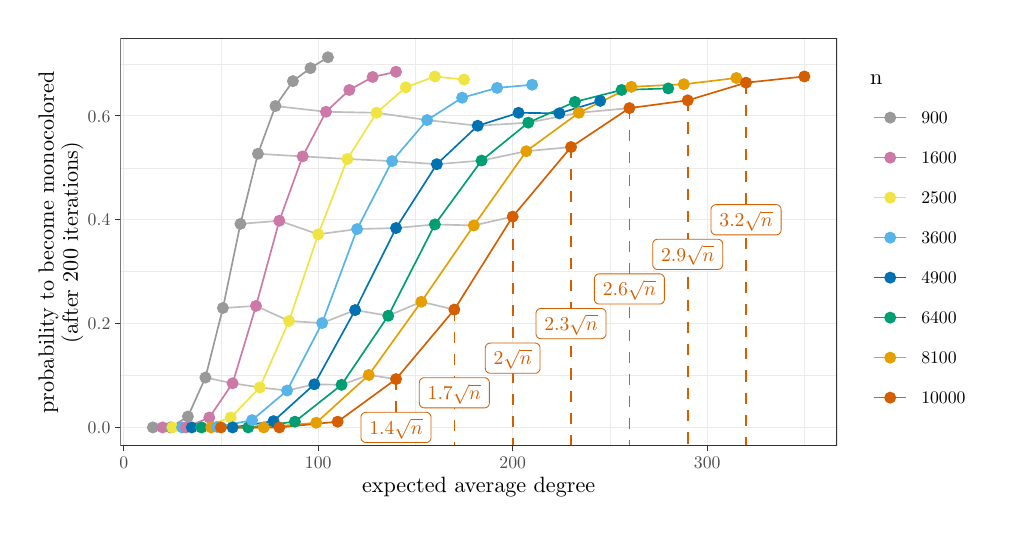
\begin{tikzpicture}[x=1pt,y=1pt]
\definecolor{fillColor}{RGB}{255,255,255}
\path[use as bounding box,fill=fillColor,fill opacity=0.00] (0,0) rectangle (346.90,173.45);
\begin{scope}
\path[clip] (  0.00,  0.00) rectangle (346.90,173.45);
\definecolor{drawColor}{RGB}{255,255,255}
\definecolor{fillColor}{RGB}{255,255,255}

\path[draw=drawColor,line width= 0.4pt,line join=round,line cap=round,fill=fillColor] (  0.00,  0.00) rectangle (346.90,173.45);
\end{scope}
\begin{scope}
\path[clip] ( 33.48, 22.32) rectangle (292.45,169.45);
\definecolor{fillColor}{RGB}{255,255,255}

\path[fill=fillColor] ( 33.48, 22.32) rectangle (292.45,169.45);
\definecolor{drawColor}{gray}{0.92}

\path[draw=drawColor,line width= 0.2pt,line join=round] ( 33.48, 47.76) --
	(292.45, 47.76);

\path[draw=drawColor,line width= 0.2pt,line join=round] ( 33.48, 85.28) --
	(292.45, 85.28);

\path[draw=drawColor,line width= 0.2pt,line join=round] ( 33.48,122.80) --
	(292.45,122.80);

\path[draw=drawColor,line width= 0.2pt,line join=round] ( 33.48,160.32) --
	(292.45,160.32);

\path[draw=drawColor,line width= 0.2pt,line join=round] ( 69.85, 22.32) --
	( 69.85,169.45);

\path[draw=drawColor,line width= 0.2pt,line join=round] (140.12, 22.32) --
	(140.12,169.45);

\path[draw=drawColor,line width= 0.2pt,line join=round] (210.40, 22.32) --
	(210.40,169.45);

\path[draw=drawColor,line width= 0.2pt,line join=round] (280.67, 22.32) --
	(280.67,169.45);

\path[draw=drawColor,line width= 0.4pt,line join=round] ( 33.48, 29.00) --
	(292.45, 29.00);

\path[draw=drawColor,line width= 0.4pt,line join=round] ( 33.48, 66.52) --
	(292.45, 66.52);

\path[draw=drawColor,line width= 0.4pt,line join=round] ( 33.48,104.04) --
	(292.45,104.04);

\path[draw=drawColor,line width= 0.4pt,line join=round] ( 33.48,141.56) --
	(292.45,141.56);

\path[draw=drawColor,line width= 0.4pt,line join=round] ( 34.71, 22.32) --
	( 34.71,169.45);

\path[draw=drawColor,line width= 0.4pt,line join=round] (104.99, 22.32) --
	(104.99,169.45);

\path[draw=drawColor,line width= 0.4pt,line join=round] (175.26, 22.32) --
	(175.26,169.45);

\path[draw=drawColor,line width= 0.4pt,line join=round] (245.54, 22.32) --
	(245.54,169.45);
\definecolor{drawColor}{RGB}{190,190,190}

\path[draw=drawColor,line width= 0.6pt,line join=round] ( 64.23, 47.01) --
	( 74.06, 44.95) --
	( 83.90, 43.45) --
	( 93.74, 42.32) --
	(103.58, 44.58) --
	(113.42, 44.39) --
	(123.26, 47.95) --
	(133.10, 46.45);

\path[draw=drawColor,line width= 0.6pt,line join=round] ( 70.55, 72.15) --
	( 82.50, 72.90) --
	( 94.44, 67.46) --
	(106.39, 66.71) --
	(118.34, 71.40) --
	(130.29, 69.34) --
	(142.23, 74.40) --
	(154.18, 71.59);

\path[draw=drawColor,line width= 0.6pt,line join=round] ( 76.88,102.54) --
	( 90.93,103.67) --
	(104.99, 98.79) --
	(119.04,100.67) --
	(133.10,101.04) --
	(147.15,102.35) --
	(161.21,101.98) --
	(175.26,105.17);

\path[draw=drawColor,line width= 0.6pt,line join=round] ( 83.20,127.87) --
	( 99.36,126.93) --
	(115.53,125.99) --
	(131.69,125.24) --
	(147.85,124.12) --
	(164.02,125.43) --
	(180.18,128.81) --
	(196.34,130.31);

\path[draw=drawColor,line width= 0.6pt,line join=round] ( 89.53,145.13) --
	(107.80,143.06) --
	(126.07,142.69) --
	(144.34,140.06) --
	(162.61,138.00) --
	(180.88,139.12) --
	(199.16,142.69) --
	(217.43,144.38);
\definecolor{drawColor}{gray}{0.60}

\path[draw=drawColor,line width= 0.6pt,line join=round] ( 45.25, 29.00) --
	( 51.58, 29.00) --
	( 57.90, 32.94) --
	( 64.23, 47.01) --
	( 70.55, 72.15) --
	( 76.88,102.54) --
	( 83.20,127.87) --
	( 89.53,145.13) --
	( 95.85,154.13) --
	(102.18,158.82) --
	(108.50,162.76);
\definecolor{drawColor}{RGB}{204,121,167}

\path[draw=drawColor,line width= 0.6pt,line join=round] ( 48.77, 29.00) --
	( 57.20, 29.00) --
	( 65.63, 32.57) --
	( 74.06, 44.95) --
	( 82.50, 72.90) --
	( 90.93,103.67) --
	( 99.36,126.93) --
	(107.80,143.06) --
	(116.23,150.94) --
	(124.66,155.63) --
	(133.10,157.51);
\definecolor{drawColor}{RGB}{240,228,66}

\path[draw=drawColor,line width= 0.6pt,line join=round] ( 52.28, 29.00) --
	( 62.82, 29.00) --
	( 73.36, 32.57) --
	( 83.90, 43.45) --
	( 94.44, 67.46) --
	(104.99, 98.79) --
	(115.53,125.99) --
	(126.07,142.69) --
	(136.61,151.88) --
	(147.15,155.82) --
	(157.69,154.69);
\definecolor{drawColor}{RGB}{86,180,233}

\path[draw=drawColor,line width= 0.6pt,line join=round] ( 55.79, 29.00) --
	( 68.44, 29.19) --
	( 81.09, 31.63) --
	( 93.74, 42.32) --
	(106.39, 66.71) --
	(119.04,100.67) --
	(131.69,125.24) --
	(144.34,140.06) --
	(156.99,148.13) --
	(169.64,151.69) --
	(182.29,152.82);
\definecolor{drawColor}{RGB}{0,114,178}

\path[draw=drawColor,line width= 0.6pt,line join=round] ( 59.31, 29.00) --
	( 74.06, 29.00) --
	( 88.82, 31.26) --
	(103.58, 44.58) --
	(118.34, 71.40) --
	(133.10,101.04) --
	(147.85,124.12) --
	(162.61,138.00) --
	(177.37,142.69) --
	(192.13,142.50) --
	(206.89,147.00);
\definecolor{drawColor}{RGB}{0,158,115}

\path[draw=drawColor,line width= 0.6pt,line join=round] ( 62.82, 29.00) --
	( 79.69, 29.00) --
	( 96.55, 31.07) --
	(113.42, 44.39) --
	(130.29, 69.34) --
	(147.15,102.35) --
	(164.02,125.43) --
	(180.88,139.12) --
	(197.75,146.63) --
	(214.62,150.94) --
	(231.48,151.50);
\definecolor{drawColor}{RGB}{230,159,0}

\path[draw=drawColor,line width= 0.6pt,line join=round] ( 66.33, 29.00) --
	( 85.31, 29.00) --
	(104.28, 30.69) --
	(123.26, 47.95) --
	(142.23, 74.40) --
	(161.21,101.98) --
	(180.18,128.81) --
	(199.16,142.69) --
	(218.13,152.07) --
	(237.10,153.01) --
	(256.08,155.26);
\definecolor{drawColor}{RGB}{213,94,0}

\path[draw=drawColor,line width= 0.6pt,line join=round] ( 69.85, 29.00) --
	( 90.93, 29.00) --
	(112.01, 31.07) --
	(133.10, 46.45) --
	(154.18, 71.59) --
	(175.26,105.17) --
	(196.34,130.31) --
	(217.43,144.38) --
	(238.51,147.19) --
	(259.59,153.57) --
	(280.67,155.82);
\definecolor{drawColor}{gray}{0.60}
\definecolor{fillColor}{gray}{0.60}

\path[draw=drawColor,line width= 0.4pt,line join=round,line cap=round,fill=fillColor] ( 45.25, 29.00) circle (  1.96);
\definecolor{drawColor}{RGB}{204,121,167}
\definecolor{fillColor}{RGB}{204,121,167}

\path[draw=drawColor,line width= 0.4pt,line join=round,line cap=round,fill=fillColor] ( 48.77, 29.00) circle (  1.96);
\definecolor{drawColor}{gray}{0.60}
\definecolor{fillColor}{gray}{0.60}

\path[draw=drawColor,line width= 0.4pt,line join=round,line cap=round,fill=fillColor] ( 51.58, 29.00) circle (  1.96);
\definecolor{drawColor}{RGB}{240,228,66}
\definecolor{fillColor}{RGB}{240,228,66}

\path[draw=drawColor,line width= 0.4pt,line join=round,line cap=round,fill=fillColor] ( 52.28, 29.00) circle (  1.96);
\definecolor{drawColor}{RGB}{86,180,233}
\definecolor{fillColor}{RGB}{86,180,233}

\path[draw=drawColor,line width= 0.4pt,line join=round,line cap=round,fill=fillColor] ( 55.79, 29.00) circle (  1.96);
\definecolor{drawColor}{RGB}{204,121,167}
\definecolor{fillColor}{RGB}{204,121,167}

\path[draw=drawColor,line width= 0.4pt,line join=round,line cap=round,fill=fillColor] ( 57.20, 29.00) circle (  1.96);
\definecolor{drawColor}{gray}{0.60}
\definecolor{fillColor}{gray}{0.60}

\path[draw=drawColor,line width= 0.4pt,line join=round,line cap=round,fill=fillColor] ( 57.90, 32.94) circle (  1.96);
\definecolor{drawColor}{RGB}{0,114,178}
\definecolor{fillColor}{RGB}{0,114,178}

\path[draw=drawColor,line width= 0.4pt,line join=round,line cap=round,fill=fillColor] ( 59.31, 29.00) circle (  1.96);
\definecolor{drawColor}{RGB}{240,228,66}
\definecolor{fillColor}{RGB}{240,228,66}

\path[draw=drawColor,line width= 0.4pt,line join=round,line cap=round,fill=fillColor] ( 62.82, 29.00) circle (  1.96);
\definecolor{drawColor}{RGB}{0,158,115}
\definecolor{fillColor}{RGB}{0,158,115}

\path[draw=drawColor,line width= 0.4pt,line join=round,line cap=round,fill=fillColor] ( 62.82, 29.00) circle (  1.96);
\definecolor{drawColor}{gray}{0.60}
\definecolor{fillColor}{gray}{0.60}

\path[draw=drawColor,line width= 0.4pt,line join=round,line cap=round,fill=fillColor] ( 64.23, 47.01) circle (  1.96);
\definecolor{drawColor}{RGB}{204,121,167}
\definecolor{fillColor}{RGB}{204,121,167}

\path[draw=drawColor,line width= 0.4pt,line join=round,line cap=round,fill=fillColor] ( 65.63, 32.57) circle (  1.96);
\definecolor{drawColor}{RGB}{230,159,0}
\definecolor{fillColor}{RGB}{230,159,0}

\path[draw=drawColor,line width= 0.4pt,line join=round,line cap=round,fill=fillColor] ( 66.33, 29.00) circle (  1.96);
\definecolor{drawColor}{RGB}{86,180,233}
\definecolor{fillColor}{RGB}{86,180,233}

\path[draw=drawColor,line width= 0.4pt,line join=round,line cap=round,fill=fillColor] ( 68.44, 29.19) circle (  1.96);
\definecolor{drawColor}{RGB}{213,94,0}
\definecolor{fillColor}{RGB}{213,94,0}

\path[draw=drawColor,line width= 0.4pt,line join=round,line cap=round,fill=fillColor] ( 69.85, 29.00) circle (  1.96);
\definecolor{drawColor}{gray}{0.60}
\definecolor{fillColor}{gray}{0.60}

\path[draw=drawColor,line width= 0.4pt,line join=round,line cap=round,fill=fillColor] ( 70.55, 72.15) circle (  1.96);
\definecolor{drawColor}{RGB}{240,228,66}
\definecolor{fillColor}{RGB}{240,228,66}

\path[draw=drawColor,line width= 0.4pt,line join=round,line cap=round,fill=fillColor] ( 73.36, 32.57) circle (  1.96);
\definecolor{drawColor}{RGB}{204,121,167}
\definecolor{fillColor}{RGB}{204,121,167}

\path[draw=drawColor,line width= 0.4pt,line join=round,line cap=round,fill=fillColor] ( 74.06, 44.95) circle (  1.96);
\definecolor{drawColor}{RGB}{0,114,178}
\definecolor{fillColor}{RGB}{0,114,178}

\path[draw=drawColor,line width= 0.4pt,line join=round,line cap=round,fill=fillColor] ( 74.06, 29.00) circle (  1.96);
\definecolor{drawColor}{gray}{0.60}
\definecolor{fillColor}{gray}{0.60}

\path[draw=drawColor,line width= 0.4pt,line join=round,line cap=round,fill=fillColor] ( 76.88,102.54) circle (  1.96);
\definecolor{drawColor}{RGB}{0,158,115}
\definecolor{fillColor}{RGB}{0,158,115}

\path[draw=drawColor,line width= 0.4pt,line join=round,line cap=round,fill=fillColor] ( 79.69, 29.00) circle (  1.96);
\definecolor{drawColor}{RGB}{86,180,233}
\definecolor{fillColor}{RGB}{86,180,233}

\path[draw=drawColor,line width= 0.4pt,line join=round,line cap=round,fill=fillColor] ( 81.09, 31.63) circle (  1.96);
\definecolor{drawColor}{RGB}{204,121,167}
\definecolor{fillColor}{RGB}{204,121,167}

\path[draw=drawColor,line width= 0.4pt,line join=round,line cap=round,fill=fillColor] ( 82.50, 72.90) circle (  1.96);
\definecolor{drawColor}{gray}{0.60}
\definecolor{fillColor}{gray}{0.60}

\path[draw=drawColor,line width= 0.4pt,line join=round,line cap=round,fill=fillColor] ( 83.20,127.87) circle (  1.96);
\definecolor{drawColor}{RGB}{240,228,66}
\definecolor{fillColor}{RGB}{240,228,66}

\path[draw=drawColor,line width= 0.4pt,line join=round,line cap=round,fill=fillColor] ( 83.90, 43.45) circle (  1.96);
\definecolor{drawColor}{RGB}{230,159,0}
\definecolor{fillColor}{RGB}{230,159,0}

\path[draw=drawColor,line width= 0.4pt,line join=round,line cap=round,fill=fillColor] ( 85.31, 29.00) circle (  1.96);
\definecolor{drawColor}{RGB}{0,114,178}
\definecolor{fillColor}{RGB}{0,114,178}

\path[draw=drawColor,line width= 0.4pt,line join=round,line cap=round,fill=fillColor] ( 88.82, 31.26) circle (  1.96);
\definecolor{drawColor}{gray}{0.60}
\definecolor{fillColor}{gray}{0.60}

\path[draw=drawColor,line width= 0.4pt,line join=round,line cap=round,fill=fillColor] ( 89.53,145.13) circle (  1.96);
\definecolor{drawColor}{RGB}{204,121,167}
\definecolor{fillColor}{RGB}{204,121,167}

\path[draw=drawColor,line width= 0.4pt,line join=round,line cap=round,fill=fillColor] ( 90.93,103.67) circle (  1.96);
\definecolor{drawColor}{RGB}{213,94,0}
\definecolor{fillColor}{RGB}{213,94,0}

\path[draw=drawColor,line width= 0.4pt,line join=round,line cap=round,fill=fillColor] ( 90.93, 29.00) circle (  1.96);
\definecolor{drawColor}{RGB}{86,180,233}
\definecolor{fillColor}{RGB}{86,180,233}

\path[draw=drawColor,line width= 0.4pt,line join=round,line cap=round,fill=fillColor] ( 93.74, 42.32) circle (  1.96);
\definecolor{drawColor}{RGB}{240,228,66}
\definecolor{fillColor}{RGB}{240,228,66}

\path[draw=drawColor,line width= 0.4pt,line join=round,line cap=round,fill=fillColor] ( 94.44, 67.46) circle (  1.96);
\definecolor{drawColor}{gray}{0.60}
\definecolor{fillColor}{gray}{0.60}

\path[draw=drawColor,line width= 0.4pt,line join=round,line cap=round,fill=fillColor] ( 95.85,154.13) circle (  1.96);
\definecolor{drawColor}{RGB}{0,158,115}
\definecolor{fillColor}{RGB}{0,158,115}

\path[draw=drawColor,line width= 0.4pt,line join=round,line cap=round,fill=fillColor] ( 96.55, 31.07) circle (  1.96);
\definecolor{drawColor}{RGB}{204,121,167}
\definecolor{fillColor}{RGB}{204,121,167}

\path[draw=drawColor,line width= 0.4pt,line join=round,line cap=round,fill=fillColor] ( 99.36,126.93) circle (  1.96);
\definecolor{drawColor}{gray}{0.60}
\definecolor{fillColor}{gray}{0.60}

\path[draw=drawColor,line width= 0.4pt,line join=round,line cap=round,fill=fillColor] (102.18,158.82) circle (  1.96);
\definecolor{drawColor}{RGB}{0,114,178}
\definecolor{fillColor}{RGB}{0,114,178}

\path[draw=drawColor,line width= 0.4pt,line join=round,line cap=round,fill=fillColor] (103.58, 44.58) circle (  1.96);
\definecolor{drawColor}{RGB}{230,159,0}
\definecolor{fillColor}{RGB}{230,159,0}

\path[draw=drawColor,line width= 0.4pt,line join=round,line cap=round,fill=fillColor] (104.28, 30.69) circle (  1.96);
\definecolor{drawColor}{RGB}{240,228,66}
\definecolor{fillColor}{RGB}{240,228,66}

\path[draw=drawColor,line width= 0.4pt,line join=round,line cap=round,fill=fillColor] (104.99, 98.79) circle (  1.96);
\definecolor{drawColor}{RGB}{86,180,233}
\definecolor{fillColor}{RGB}{86,180,233}

\path[draw=drawColor,line width= 0.4pt,line join=round,line cap=round,fill=fillColor] (106.39, 66.71) circle (  1.96);
\definecolor{drawColor}{RGB}{204,121,167}
\definecolor{fillColor}{RGB}{204,121,167}

\path[draw=drawColor,line width= 0.4pt,line join=round,line cap=round,fill=fillColor] (107.80,143.06) circle (  1.96);
\definecolor{drawColor}{gray}{0.60}
\definecolor{fillColor}{gray}{0.60}

\path[draw=drawColor,line width= 0.4pt,line join=round,line cap=round,fill=fillColor] (108.50,162.76) circle (  1.96);
\definecolor{drawColor}{RGB}{213,94,0}
\definecolor{fillColor}{RGB}{213,94,0}

\path[draw=drawColor,line width= 0.4pt,line join=round,line cap=round,fill=fillColor] (112.01, 31.07) circle (  1.96);
\definecolor{drawColor}{RGB}{0,158,115}
\definecolor{fillColor}{RGB}{0,158,115}

\path[draw=drawColor,line width= 0.4pt,line join=round,line cap=round,fill=fillColor] (113.42, 44.39) circle (  1.96);
\definecolor{drawColor}{RGB}{240,228,66}
\definecolor{fillColor}{RGB}{240,228,66}

\path[draw=drawColor,line width= 0.4pt,line join=round,line cap=round,fill=fillColor] (115.53,125.99) circle (  1.96);
\definecolor{drawColor}{RGB}{204,121,167}
\definecolor{fillColor}{RGB}{204,121,167}

\path[draw=drawColor,line width= 0.4pt,line join=round,line cap=round,fill=fillColor] (116.23,150.94) circle (  1.96);
\definecolor{drawColor}{RGB}{0,114,178}
\definecolor{fillColor}{RGB}{0,114,178}

\path[draw=drawColor,line width= 0.4pt,line join=round,line cap=round,fill=fillColor] (118.34, 71.40) circle (  1.96);
\definecolor{drawColor}{RGB}{86,180,233}
\definecolor{fillColor}{RGB}{86,180,233}

\path[draw=drawColor,line width= 0.4pt,line join=round,line cap=round,fill=fillColor] (119.04,100.67) circle (  1.96);
\definecolor{drawColor}{RGB}{230,159,0}
\definecolor{fillColor}{RGB}{230,159,0}

\path[draw=drawColor,line width= 0.4pt,line join=round,line cap=round,fill=fillColor] (123.26, 47.95) circle (  1.96);
\definecolor{drawColor}{RGB}{204,121,167}
\definecolor{fillColor}{RGB}{204,121,167}

\path[draw=drawColor,line width= 0.4pt,line join=round,line cap=round,fill=fillColor] (124.66,155.63) circle (  1.96);
\definecolor{drawColor}{RGB}{240,228,66}
\definecolor{fillColor}{RGB}{240,228,66}

\path[draw=drawColor,line width= 0.4pt,line join=round,line cap=round,fill=fillColor] (126.07,142.69) circle (  1.96);
\definecolor{drawColor}{RGB}{0,158,115}
\definecolor{fillColor}{RGB}{0,158,115}

\path[draw=drawColor,line width= 0.4pt,line join=round,line cap=round,fill=fillColor] (130.29, 69.34) circle (  1.96);
\definecolor{drawColor}{RGB}{86,180,233}
\definecolor{fillColor}{RGB}{86,180,233}

\path[draw=drawColor,line width= 0.4pt,line join=round,line cap=round,fill=fillColor] (131.69,125.24) circle (  1.96);
\definecolor{drawColor}{RGB}{204,121,167}
\definecolor{fillColor}{RGB}{204,121,167}

\path[draw=drawColor,line width= 0.4pt,line join=round,line cap=round,fill=fillColor] (133.10,157.51) circle (  1.96);
\definecolor{drawColor}{RGB}{0,114,178}
\definecolor{fillColor}{RGB}{0,114,178}

\path[draw=drawColor,line width= 0.4pt,line join=round,line cap=round,fill=fillColor] (133.10,101.04) circle (  1.96);
\definecolor{drawColor}{RGB}{213,94,0}
\definecolor{fillColor}{RGB}{213,94,0}

\path[draw=drawColor,line width= 0.4pt,line join=round,line cap=round,fill=fillColor] (133.10, 46.45) circle (  1.96);
\definecolor{drawColor}{RGB}{240,228,66}
\definecolor{fillColor}{RGB}{240,228,66}

\path[draw=drawColor,line width= 0.4pt,line join=round,line cap=round,fill=fillColor] (136.61,151.88) circle (  1.96);
\definecolor{drawColor}{RGB}{230,159,0}
\definecolor{fillColor}{RGB}{230,159,0}

\path[draw=drawColor,line width= 0.4pt,line join=round,line cap=round,fill=fillColor] (142.23, 74.40) circle (  1.96);
\definecolor{drawColor}{RGB}{86,180,233}
\definecolor{fillColor}{RGB}{86,180,233}

\path[draw=drawColor,line width= 0.4pt,line join=round,line cap=round,fill=fillColor] (144.34,140.06) circle (  1.96);
\definecolor{drawColor}{RGB}{240,228,66}
\definecolor{fillColor}{RGB}{240,228,66}

\path[draw=drawColor,line width= 0.4pt,line join=round,line cap=round,fill=fillColor] (147.15,155.82) circle (  1.96);
\definecolor{drawColor}{RGB}{0,158,115}
\definecolor{fillColor}{RGB}{0,158,115}

\path[draw=drawColor,line width= 0.4pt,line join=round,line cap=round,fill=fillColor] (147.15,102.35) circle (  1.96);
\definecolor{drawColor}{RGB}{0,114,178}
\definecolor{fillColor}{RGB}{0,114,178}

\path[draw=drawColor,line width= 0.4pt,line join=round,line cap=round,fill=fillColor] (147.85,124.12) circle (  1.96);
\definecolor{drawColor}{RGB}{213,94,0}
\definecolor{fillColor}{RGB}{213,94,0}

\path[draw=drawColor,line width= 0.4pt,line join=round,line cap=round,fill=fillColor] (154.18, 71.59) circle (  1.96);
\definecolor{drawColor}{RGB}{86,180,233}
\definecolor{fillColor}{RGB}{86,180,233}

\path[draw=drawColor,line width= 0.4pt,line join=round,line cap=round,fill=fillColor] (156.99,148.13) circle (  1.96);
\definecolor{drawColor}{RGB}{240,228,66}
\definecolor{fillColor}{RGB}{240,228,66}

\path[draw=drawColor,line width= 0.4pt,line join=round,line cap=round,fill=fillColor] (157.69,154.69) circle (  1.96);
\definecolor{drawColor}{RGB}{230,159,0}
\definecolor{fillColor}{RGB}{230,159,0}

\path[draw=drawColor,line width= 0.4pt,line join=round,line cap=round,fill=fillColor] (161.21,101.98) circle (  1.96);
\definecolor{drawColor}{RGB}{0,114,178}
\definecolor{fillColor}{RGB}{0,114,178}

\path[draw=drawColor,line width= 0.4pt,line join=round,line cap=round,fill=fillColor] (162.61,138.00) circle (  1.96);
\definecolor{drawColor}{RGB}{0,158,115}
\definecolor{fillColor}{RGB}{0,158,115}

\path[draw=drawColor,line width= 0.4pt,line join=round,line cap=round,fill=fillColor] (164.02,125.43) circle (  1.96);
\definecolor{drawColor}{RGB}{86,180,233}
\definecolor{fillColor}{RGB}{86,180,233}

\path[draw=drawColor,line width= 0.4pt,line join=round,line cap=round,fill=fillColor] (169.64,151.69) circle (  1.96);
\definecolor{drawColor}{RGB}{213,94,0}
\definecolor{fillColor}{RGB}{213,94,0}

\path[draw=drawColor,line width= 0.4pt,line join=round,line cap=round,fill=fillColor] (175.26,105.17) circle (  1.96);
\definecolor{drawColor}{RGB}{0,114,178}
\definecolor{fillColor}{RGB}{0,114,178}

\path[draw=drawColor,line width= 0.4pt,line join=round,line cap=round,fill=fillColor] (177.37,142.69) circle (  1.96);
\definecolor{drawColor}{RGB}{230,159,0}
\definecolor{fillColor}{RGB}{230,159,0}

\path[draw=drawColor,line width= 0.4pt,line join=round,line cap=round,fill=fillColor] (180.18,128.81) circle (  1.96);
\definecolor{drawColor}{RGB}{0,158,115}
\definecolor{fillColor}{RGB}{0,158,115}

\path[draw=drawColor,line width= 0.4pt,line join=round,line cap=round,fill=fillColor] (180.88,139.12) circle (  1.96);
\definecolor{drawColor}{RGB}{86,180,233}
\definecolor{fillColor}{RGB}{86,180,233}

\path[draw=drawColor,line width= 0.4pt,line join=round,line cap=round,fill=fillColor] (182.29,152.82) circle (  1.96);
\definecolor{drawColor}{RGB}{0,114,178}
\definecolor{fillColor}{RGB}{0,114,178}

\path[draw=drawColor,line width= 0.4pt,line join=round,line cap=round,fill=fillColor] (192.13,142.50) circle (  1.96);
\definecolor{drawColor}{RGB}{213,94,0}
\definecolor{fillColor}{RGB}{213,94,0}

\path[draw=drawColor,line width= 0.4pt,line join=round,line cap=round,fill=fillColor] (196.34,130.31) circle (  1.96);
\definecolor{drawColor}{RGB}{0,158,115}
\definecolor{fillColor}{RGB}{0,158,115}

\path[draw=drawColor,line width= 0.4pt,line join=round,line cap=round,fill=fillColor] (197.75,146.63) circle (  1.96);
\definecolor{drawColor}{RGB}{230,159,0}
\definecolor{fillColor}{RGB}{230,159,0}

\path[draw=drawColor,line width= 0.4pt,line join=round,line cap=round,fill=fillColor] (199.16,142.69) circle (  1.96);
\definecolor{drawColor}{RGB}{0,114,178}
\definecolor{fillColor}{RGB}{0,114,178}

\path[draw=drawColor,line width= 0.4pt,line join=round,line cap=round,fill=fillColor] (206.89,147.00) circle (  1.96);
\definecolor{drawColor}{RGB}{0,158,115}
\definecolor{fillColor}{RGB}{0,158,115}

\path[draw=drawColor,line width= 0.4pt,line join=round,line cap=round,fill=fillColor] (214.62,150.94) circle (  1.96);
\definecolor{drawColor}{RGB}{213,94,0}
\definecolor{fillColor}{RGB}{213,94,0}

\path[draw=drawColor,line width= 0.4pt,line join=round,line cap=round,fill=fillColor] (217.43,144.38) circle (  1.96);
\definecolor{drawColor}{RGB}{230,159,0}
\definecolor{fillColor}{RGB}{230,159,0}

\path[draw=drawColor,line width= 0.4pt,line join=round,line cap=round,fill=fillColor] (218.13,152.07) circle (  1.96);
\definecolor{drawColor}{RGB}{0,158,115}
\definecolor{fillColor}{RGB}{0,158,115}

\path[draw=drawColor,line width= 0.4pt,line join=round,line cap=round,fill=fillColor] (231.48,151.50) circle (  1.96);
\definecolor{drawColor}{RGB}{230,159,0}
\definecolor{fillColor}{RGB}{230,159,0}

\path[draw=drawColor,line width= 0.4pt,line join=round,line cap=round,fill=fillColor] (237.10,153.01) circle (  1.96);
\definecolor{drawColor}{RGB}{213,94,0}
\definecolor{fillColor}{RGB}{213,94,0}

\path[draw=drawColor,line width= 0.4pt,line join=round,line cap=round,fill=fillColor] (238.51,147.19) circle (  1.96);
\definecolor{drawColor}{RGB}{230,159,0}
\definecolor{fillColor}{RGB}{230,159,0}

\path[draw=drawColor,line width= 0.4pt,line join=round,line cap=round,fill=fillColor] (256.08,155.26) circle (  1.96);
\definecolor{drawColor}{RGB}{213,94,0}
\definecolor{fillColor}{RGB}{213,94,0}

\path[draw=drawColor,line width= 0.4pt,line join=round,line cap=round,fill=fillColor] (259.59,153.57) circle (  1.96);

\path[draw=drawColor,line width= 0.4pt,line join=round,line cap=round,fill=fillColor] (280.67,155.82) circle (  1.96);

\path[draw=drawColor,line width= 0.6pt,dash pattern=on 4pt off 4pt ,line join=round] (133.10, 46.45) -- (133.10, 22.32);

\path[draw=drawColor,line width= 0.6pt,dash pattern=on 4pt off 4pt ,line join=round] (154.18, 71.59) -- (154.18, 22.32);

\path[draw=drawColor,line width= 0.6pt,dash pattern=on 4pt off 4pt ,line join=round] (175.26,105.17) -- (175.26, 22.32);

\path[draw=drawColor,line width= 0.6pt,dash pattern=on 4pt off 4pt ,line join=round] (196.34,130.31) -- (196.34, 22.32);

\path[draw=drawColor,line width= 0.6pt,dash pattern=on 4pt off 4pt ,line join=round] (217.43,144.38) -- (217.43, 22.32);

\path[draw=drawColor,line width= 0.6pt,dash pattern=on 4pt off 4pt ,line join=round] (238.51,147.19) -- (238.51, 22.32);

\path[draw=drawColor,line width= 0.6pt,dash pattern=on 4pt off 4pt ,line join=round] (259.59,153.57) -- (259.59, 22.32);
\definecolor{fillColor}{RGB}{255,255,255}

\path[draw=drawColor,line width= 0.3pt,line join=round,line cap=round,fill=fillColor] (122.25, 23.54) --
	(143.94, 23.54) --
	(143.87, 23.55) --
	(144.16, 23.56) --
	(144.45, 23.62) --
	(144.72, 23.72) --
	(144.97, 23.86) --
	(145.20, 24.05) --
	(145.39, 24.27) --
	(145.54, 24.51) --
	(145.66, 24.78) --
	(145.73, 25.06) --
	(145.75, 25.35) --
	(145.75, 25.35) --
	(145.75, 32.66) --
	(145.75, 32.66) --
	(145.73, 32.95) --
	(145.66, 33.23) --
	(145.54, 33.50) --
	(145.39, 33.74) --
	(145.20, 33.96) --
	(144.97, 34.15) --
	(144.72, 34.29) --
	(144.45, 34.39) --
	(144.16, 34.45) --
	(143.94, 34.47) --
	(122.25, 34.47) --
	(122.47, 34.45) --
	(122.18, 34.46) --
	(121.89, 34.43) --
	(121.61, 34.35) --
	(121.35, 34.22) --
	(121.11, 34.06) --
	(120.90, 33.86) --
	(120.72, 33.62) --
	(120.59, 33.37) --
	(120.49, 33.09) --
	(120.45, 32.80) --
	(120.44, 32.66) --
	(120.44, 25.35) --
	(120.45, 25.50) --
	(120.45, 25.21) --
	(120.49, 24.92) --
	(120.59, 24.64) --
	(120.72, 24.39) --
	(120.90, 24.15) --
	(121.11, 23.95) --
	(121.35, 23.79) --
	(121.61, 23.66) --
	(121.89, 23.58) --
	(122.18, 23.55) --
	cycle;
\end{scope}
\begin{scope}
\path[clip] ( 33.48, 22.32) rectangle (292.45,169.45);
\definecolor{drawColor}{RGB}{213,94,0}

\node[text=drawColor,anchor=base,inner sep=0pt, outer sep=0pt, scale=  0.71] at (133.10, 26.56) {$1.4\sqrt{n}$};
\definecolor{fillColor}{RGB}{255,255,255}

\path[draw=drawColor,line width= 0.3pt,line join=round,line cap=round,fill=fillColor] (143.33, 36.05) --
	(165.03, 36.05) --
	(164.95, 36.05) --
	(165.24, 36.06) --
	(165.53, 36.12) --
	(165.80, 36.22) --
	(166.05, 36.37) --
	(166.28, 36.55) --
	(166.47, 36.77) --
	(166.63, 37.02) --
	(166.74, 37.28) --
	(166.81, 37.57) --
	(166.83, 37.86) --
	(166.83, 37.86) --
	(166.83, 45.16) --
	(166.83, 45.16) --
	(166.81, 45.45) --
	(166.74, 45.74) --
	(166.63, 46.00) --
	(166.47, 46.25) --
	(166.28, 46.47) --
	(166.05, 46.65) --
	(165.80, 46.80) --
	(165.53, 46.90) --
	(165.24, 46.96) --
	(165.03, 46.97) --
	(143.33, 46.97) --
	(143.55, 46.96) --
	(143.26, 46.97) --
	(142.97, 46.94) --
	(142.69, 46.85) --
	(142.43, 46.73) --
	(142.19, 46.56) --
	(141.98, 46.36) --
	(141.80, 46.13) --
	(141.67, 45.87) --
	(141.58, 45.60) --
	(141.53, 45.31) --
	(141.52, 45.16) --
	(141.52, 37.86) --
	(141.53, 38.00) --
	(141.53, 37.71) --
	(141.58, 37.42) --
	(141.67, 37.15) --
	(141.80, 36.89) --
	(141.98, 36.66) --
	(142.19, 36.46) --
	(142.43, 36.29) --
	(142.69, 36.17) --
	(142.97, 36.09) --
	(143.26, 36.05) --
	cycle;
\end{scope}
\begin{scope}
\path[clip] ( 33.48, 22.32) rectangle (292.45,169.45);
\definecolor{drawColor}{RGB}{213,94,0}

\node[text=drawColor,anchor=base,inner sep=0pt, outer sep=0pt, scale=  0.71] at (154.18, 39.06) {$1.7\sqrt{n}$};
\definecolor{fillColor}{RGB}{255,255,255}

\path[draw=drawColor,line width= 0.3pt,line join=round,line cap=round,fill=fillColor] (167.18, 48.56) --
	(183.34, 48.56) --
	(183.27, 48.56) --
	(183.56, 48.57) --
	(183.85, 48.63) --
	(184.12, 48.73) --
	(184.37, 48.88) --
	(184.59, 49.06) --
	(184.79, 49.28) --
	(184.94, 49.52) --
	(185.06, 49.79) --
	(185.13, 50.07) --
	(185.15, 50.36) --
	(185.15, 50.36) --
	(185.15, 57.67) --
	(185.15, 57.67) --
	(185.13, 57.96) --
	(185.06, 58.24) --
	(184.94, 58.51) --
	(184.79, 58.76) --
	(184.59, 58.97) --
	(184.37, 59.16) --
	(184.12, 59.30) --
	(183.85, 59.41) --
	(183.56, 59.46) --
	(183.34, 59.48) --
	(167.18, 59.48) --
	(167.40, 59.46) --
	(167.11, 59.48) --
	(166.82, 59.44) --
	(166.54, 59.36) --
	(166.28, 59.24) --
	(166.04, 59.07) --
	(165.83, 58.87) --
	(165.65, 58.64) --
	(165.52, 58.38) --
	(165.43, 58.10) --
	(165.38, 57.82) --
	(165.37, 57.67) --
	(165.37, 50.36) --
	(165.38, 50.51) --
	(165.38, 50.22) --
	(165.43, 49.93) --
	(165.52, 49.66) --
	(165.65, 49.40) --
	(165.83, 49.17) --
	(166.04, 48.96) --
	(166.28, 48.80) --
	(166.54, 48.67) --
	(166.82, 48.59) --
	(167.11, 48.56) --
	cycle;
\end{scope}
\begin{scope}
\path[clip] ( 33.48, 22.32) rectangle (292.45,169.45);
\definecolor{drawColor}{RGB}{213,94,0}

\node[text=drawColor,anchor=base,inner sep=0pt, outer sep=0pt, scale=  0.71] at (175.26, 51.57) {$2\sqrt{n}$};
\definecolor{fillColor}{RGB}{255,255,255}

\path[draw=drawColor,line width= 0.3pt,line join=round,line cap=round,fill=fillColor] (185.50, 61.06) --
	(207.19, 61.06) --
	(207.12, 61.06) --
	(207.41, 61.08) --
	(207.69, 61.13) --
	(207.97, 61.24) --
	(208.22, 61.38) --
	(208.44, 61.57) --
	(208.64, 61.78) --
	(208.79, 62.03) --
	(208.91, 62.30) --
	(208.98, 62.58) --
	(209.00, 62.87) --
	(209.00, 62.87) --
	(209.00, 70.18) --
	(209.00, 70.18) --
	(208.98, 70.47) --
	(208.91, 70.75) --
	(208.79, 71.02) --
	(208.64, 71.26) --
	(208.44, 71.48) --
	(208.22, 71.66) --
	(207.97, 71.81) --
	(207.69, 71.91) --
	(207.41, 71.97) --
	(207.19, 71.98) --
	(185.50, 71.98) --
	(185.71, 71.97) --
	(185.42, 71.98) --
	(185.14, 71.95) --
	(184.86, 71.87) --
	(184.59, 71.74) --
	(184.35, 71.58) --
	(184.14, 71.38) --
	(183.97, 71.14) --
	(183.83, 70.89) --
	(183.74, 70.61) --
	(183.70, 70.32) --
	(183.69, 70.18) --
	(183.69, 62.87) --
	(183.70, 63.02) --
	(183.70, 62.72) --
	(183.74, 62.44) --
	(183.83, 62.16) --
	(183.97, 61.90) --
	(184.14, 61.67) --
	(184.35, 61.47) --
	(184.59, 61.31) --
	(184.86, 61.18) --
	(185.14, 61.10) --
	(185.42, 61.06) --
	cycle;
\end{scope}
\begin{scope}
\path[clip] ( 33.48, 22.32) rectangle (292.45,169.45);
\definecolor{drawColor}{RGB}{213,94,0}

\node[text=drawColor,anchor=base,inner sep=0pt, outer sep=0pt, scale=  0.71] at (196.34, 64.07) {$2.3\sqrt{n}$};
\definecolor{fillColor}{RGB}{255,255,255}

\path[draw=drawColor,line width= 0.3pt,line join=round,line cap=round,fill=fillColor] (206.58, 73.57) --
	(228.27, 73.57) --
	(228.20, 73.57) --
	(228.49, 73.58) --
	(228.78, 73.64) --
	(229.05, 73.74) --
	(229.30, 73.89) --
	(229.53, 74.07) --
	(229.72, 74.29) --
	(229.87, 74.54) --
	(229.99, 74.80) --
	(230.06, 75.09) --
	(230.08, 75.38) --
	(230.08, 75.38) --
	(230.08, 82.68) --
	(230.08, 82.68) --
	(230.06, 82.97) --
	(229.99, 83.26) --
	(229.87, 83.52) --
	(229.72, 83.77) --
	(229.53, 83.99) --
	(229.30, 84.17) --
	(229.05, 84.32) --
	(228.78, 84.42) --
	(228.49, 84.48) --
	(228.27, 84.49) --
	(206.58, 84.49) --
	(206.80, 84.48) --
	(206.51, 84.49) --
	(206.22, 84.45) --
	(205.94, 84.37) --
	(205.68, 84.25) --
	(205.44, 84.08) --
	(205.23, 83.88) --
	(205.05, 83.65) --
	(204.92, 83.39) --
	(204.83, 83.12) --
	(204.78, 82.83) --
	(204.77, 82.68) --
	(204.77, 75.38) --
	(204.78, 75.52) --
	(204.78, 75.23) --
	(204.83, 74.94) --
	(204.92, 74.67) --
	(205.05, 74.41) --
	(205.23, 74.18) --
	(205.44, 73.98) --
	(205.68, 73.81) --
	(205.94, 73.69) --
	(206.22, 73.61) --
	(206.51, 73.57) --
	cycle;
\end{scope}
\begin{scope}
\path[clip] ( 33.48, 22.32) rectangle (292.45,169.45);
\definecolor{drawColor}{RGB}{213,94,0}

\node[text=drawColor,anchor=base,inner sep=0pt, outer sep=0pt, scale=  0.71] at (217.43, 76.58) {$2.6\sqrt{n}$};
\definecolor{fillColor}{RGB}{255,255,255}

\path[draw=drawColor,line width= 0.3pt,line join=round,line cap=round,fill=fillColor] (227.66, 86.08) --
	(249.36, 86.08) --
	(249.28, 86.08) --
	(249.57, 86.09) --
	(249.86, 86.15) --
	(250.13, 86.25) --
	(250.38, 86.40) --
	(250.61, 86.58) --
	(250.80, 86.80) --
	(250.96, 87.04) --
	(251.07, 87.31) --
	(251.14, 87.59) --
	(251.16, 87.88) --
	(251.16, 87.88) --
	(251.16, 95.19) --
	(251.16, 95.19) --
	(251.14, 95.48) --
	(251.07, 95.76) --
	(250.96, 96.03) --
	(250.80, 96.28) --
	(250.61, 96.49) --
	(250.38, 96.68) --
	(250.13, 96.82) --
	(249.86, 96.93) --
	(249.57, 96.98) --
	(249.36, 97.00) --
	(227.66, 97.00) --
	(227.88, 96.98) --
	(227.59, 97.00) --
	(227.30, 96.96) --
	(227.02, 96.88) --
	(226.76, 96.76) --
	(226.52, 96.59) --
	(226.31, 96.39) --
	(226.13, 96.16) --
	(226.00, 95.90) --
	(225.91, 95.62) --
	(225.86, 95.34) --
	(225.86, 95.19) --
	(225.86, 87.88) --
	(225.86, 88.03) --
	(225.86, 87.74) --
	(225.91, 87.45) --
	(226.00, 87.17) --
	(226.13, 86.92) --
	(226.31, 86.68) --
	(226.52, 86.48) --
	(226.76, 86.32) --
	(227.02, 86.19) --
	(227.30, 86.11) --
	(227.59, 86.08) --
	cycle;
\end{scope}
\begin{scope}
\path[clip] ( 33.48, 22.32) rectangle (292.45,169.45);
\definecolor{drawColor}{RGB}{213,94,0}

\node[text=drawColor,anchor=base,inner sep=0pt, outer sep=0pt, scale=  0.71] at (238.51, 89.09) {$2.9\sqrt{n}$};
\definecolor{fillColor}{RGB}{255,255,255}

\path[draw=drawColor,line width= 0.3pt,line join=round,line cap=round,fill=fillColor] (248.74, 98.58) --
	(270.44, 98.58) --
	(270.37, 98.58) --
	(270.66, 98.60) --
	(270.94, 98.65) --
	(271.21, 98.76) --
	(271.47, 98.90) --
	(271.69, 99.09) --
	(271.88, 99.30) --
	(272.04, 99.55) --
	(272.15, 99.82) --
	(272.22,100.10) --
	(272.25,100.39) --
	(272.25,100.39) --
	(272.25,107.70) --
	(272.25,107.70) --
	(272.22,107.99) --
	(272.15,108.27) --
	(272.04,108.54) --
	(271.88,108.78) --
	(271.69,109.00) --
	(271.47,109.18) --
	(271.21,109.33) --
	(270.94,109.43) --
	(270.66,109.49) --
	(270.44,109.50) --
	(248.74,109.50) --
	(248.96,109.49) --
	(248.67,109.50) --
	(248.38,109.47) --
	(248.10,109.39) --
	(247.84,109.26) --
	(247.60,109.10) --
	(247.39,108.89) --
	(247.22,108.66) --
	(247.08,108.40) --
	(246.99,108.13) --
	(246.94,107.84) --
	(246.94,107.70) --
	(246.94,100.39) --
	(246.94,100.53) --
	(246.94,100.24) --
	(246.99, 99.96) --
	(247.08, 99.68) --
	(247.22, 99.42) --
	(247.39, 99.19) --
	(247.60, 98.99) --
	(247.84, 98.82) --
	(248.10, 98.70) --
	(248.38, 98.62) --
	(248.67, 98.58) --
	cycle;
\end{scope}
\begin{scope}
\path[clip] ( 33.48, 22.32) rectangle (292.45,169.45);
\definecolor{drawColor}{RGB}{213,94,0}

\node[text=drawColor,anchor=base,inner sep=0pt, outer sep=0pt, scale=  0.71] at (259.59,101.59) {$3.2\sqrt{n}$};
\definecolor{drawColor}{gray}{0.20}

\path[draw=drawColor,line width= 0.4pt,line join=round,line cap=round] ( 33.48, 22.32) rectangle (292.45,169.45);
\end{scope}
\begin{scope}
\path[clip] (  0.00,  0.00) rectangle (346.90,173.45);
\definecolor{drawColor}{gray}{0.30}

\node[text=drawColor,anchor=base east,inner sep=0pt, outer sep=0pt, scale=  0.64] at ( 29.88, 26.80) {0.0};

\node[text=drawColor,anchor=base east,inner sep=0pt, outer sep=0pt, scale=  0.64] at ( 29.88, 64.32) {0.2};

\node[text=drawColor,anchor=base east,inner sep=0pt, outer sep=0pt, scale=  0.64] at ( 29.88,101.84) {0.4};

\node[text=drawColor,anchor=base east,inner sep=0pt, outer sep=0pt, scale=  0.64] at ( 29.88,139.36) {0.6};
\end{scope}
\begin{scope}
\path[clip] (  0.00,  0.00) rectangle (346.90,173.45);
\definecolor{drawColor}{gray}{0.20}

\path[draw=drawColor,line width= 0.4pt,line join=round] ( 31.48, 29.00) --
	( 33.48, 29.00);

\path[draw=drawColor,line width= 0.4pt,line join=round] ( 31.48, 66.52) --
	( 33.48, 66.52);

\path[draw=drawColor,line width= 0.4pt,line join=round] ( 31.48,104.04) --
	( 33.48,104.04);

\path[draw=drawColor,line width= 0.4pt,line join=round] ( 31.48,141.56) --
	( 33.48,141.56);
\end{scope}
\begin{scope}
\path[clip] (  0.00,  0.00) rectangle (346.90,173.45);
\definecolor{drawColor}{gray}{0.20}

\path[draw=drawColor,line width= 0.4pt,line join=round] ( 34.71, 20.32) --
	( 34.71, 22.32);

\path[draw=drawColor,line width= 0.4pt,line join=round] (104.99, 20.32) --
	(104.99, 22.32);

\path[draw=drawColor,line width= 0.4pt,line join=round] (175.26, 20.32) --
	(175.26, 22.32);

\path[draw=drawColor,line width= 0.4pt,line join=round] (245.54, 20.32) --
	(245.54, 22.32);
\end{scope}
\begin{scope}
\path[clip] (  0.00,  0.00) rectangle (346.90,173.45);
\definecolor{drawColor}{gray}{0.30}

\node[text=drawColor,anchor=base,inner sep=0pt, outer sep=0pt, scale=  0.64] at ( 34.71, 14.31) {0};

\node[text=drawColor,anchor=base,inner sep=0pt, outer sep=0pt, scale=  0.64] at (104.99, 14.31) {100};

\node[text=drawColor,anchor=base,inner sep=0pt, outer sep=0pt, scale=  0.64] at (175.26, 14.31) {200};

\node[text=drawColor,anchor=base,inner sep=0pt, outer sep=0pt, scale=  0.64] at (245.54, 14.31) {300};
\end{scope}
\begin{scope}
\path[clip] (  0.00,  0.00) rectangle (346.90,173.45);
\definecolor{drawColor}{RGB}{0,0,0}

\node[text=drawColor,anchor=base,inner sep=0pt, outer sep=0pt, scale=  0.80] at (162.96,  5.56) {expected average degree};
\end{scope}
\begin{scope}
\path[clip] (  0.00,  0.00) rectangle (346.90,173.45);
\definecolor{drawColor}{RGB}{0,0,0}

\node[text=drawColor,rotate= 90.00,anchor=base,inner sep=0pt, outer sep=0pt, scale=  0.80] at (  9.51, 95.88) {probability to become monocolored};

\node[text=drawColor,rotate= 90.00,anchor=base,inner sep=0pt, outer sep=0pt, scale=  0.80] at ( 18.15, 95.88) {(after 200 iterations)};
\end{scope}
\begin{scope}
\path[clip] (  0.00,  0.00) rectangle (346.90,173.45);
\definecolor{fillColor}{RGB}{255,255,255}

\path[fill=fillColor] (300.45, 28.53) rectangle (342.90,163.23);
\end{scope}
\begin{scope}
\path[clip] (  0.00,  0.00) rectangle (346.90,173.45);
\definecolor{drawColor}{RGB}{0,0,0}

\node[text=drawColor,anchor=base west,inner sep=0pt, outer sep=0pt, scale=  0.80] at (304.45,152.94) {n};
\end{scope}
\begin{scope}
\path[clip] (  0.00,  0.00) rectangle (346.90,173.45);
\definecolor{fillColor}{RGB}{255,255,255}

\path[fill=fillColor] (304.45,133.71) rectangle (318.90,148.17);
\end{scope}
\begin{scope}
\path[clip] (  0.00,  0.00) rectangle (346.90,173.45);
\definecolor{drawColor}{gray}{0.60}

\path[draw=drawColor,line width= 0.6pt,line join=round] (305.89,140.94) -- (317.45,140.94);
\end{scope}
\begin{scope}
\path[clip] (  0.00,  0.00) rectangle (346.90,173.45);
\definecolor{drawColor}{gray}{0.60}
\definecolor{fillColor}{gray}{0.60}

\path[draw=drawColor,line width= 0.4pt,line join=round,line cap=round,fill=fillColor] (311.67,140.94) circle (  1.96);
\end{scope}
\begin{scope}
\path[clip] (  0.00,  0.00) rectangle (346.90,173.45);
\definecolor{drawColor}{gray}{0.60}

\path[draw=drawColor,line width= 0.6pt,dash pattern=on 4pt off 4pt ,line join=round] (305.89,140.94) -- (317.45,140.94);
\end{scope}
\begin{scope}
\path[clip] (  0.00,  0.00) rectangle (346.90,173.45);
\definecolor{fillColor}{RGB}{255,255,255}

\path[fill=fillColor] (304.45,119.26) rectangle (318.90,133.71);
\end{scope}
\begin{scope}
\path[clip] (  0.00,  0.00) rectangle (346.90,173.45);
\definecolor{drawColor}{RGB}{204,121,167}

\path[draw=drawColor,line width= 0.6pt,line join=round] (305.89,126.48) -- (317.45,126.48);
\end{scope}
\begin{scope}
\path[clip] (  0.00,  0.00) rectangle (346.90,173.45);
\definecolor{drawColor}{RGB}{204,121,167}
\definecolor{fillColor}{RGB}{204,121,167}

\path[draw=drawColor,line width= 0.4pt,line join=round,line cap=round,fill=fillColor] (311.67,126.48) circle (  1.96);
\end{scope}
\begin{scope}
\path[clip] (  0.00,  0.00) rectangle (346.90,173.45);
\definecolor{drawColor}{RGB}{204,121,167}

\path[draw=drawColor,line width= 0.6pt,dash pattern=on 4pt off 4pt ,line join=round] (305.89,126.48) -- (317.45,126.48);
\end{scope}
\begin{scope}
\path[clip] (  0.00,  0.00) rectangle (346.90,173.45);
\definecolor{fillColor}{RGB}{255,255,255}

\path[fill=fillColor] (304.45,104.80) rectangle (318.90,119.26);
\end{scope}
\begin{scope}
\path[clip] (  0.00,  0.00) rectangle (346.90,173.45);
\definecolor{drawColor}{RGB}{240,228,66}

\path[draw=drawColor,line width= 0.6pt,line join=round] (305.89,112.03) -- (317.45,112.03);
\end{scope}
\begin{scope}
\path[clip] (  0.00,  0.00) rectangle (346.90,173.45);
\definecolor{drawColor}{RGB}{240,228,66}
\definecolor{fillColor}{RGB}{240,228,66}

\path[draw=drawColor,line width= 0.4pt,line join=round,line cap=round,fill=fillColor] (311.67,112.03) circle (  1.96);
\end{scope}
\begin{scope}
\path[clip] (  0.00,  0.00) rectangle (346.90,173.45);
\definecolor{drawColor}{RGB}{240,228,66}

\path[draw=drawColor,line width= 0.6pt,dash pattern=on 4pt off 4pt ,line join=round] (305.89,112.03) -- (317.45,112.03);
\end{scope}
\begin{scope}
\path[clip] (  0.00,  0.00) rectangle (346.90,173.45);
\definecolor{fillColor}{RGB}{255,255,255}

\path[fill=fillColor] (304.45, 90.35) rectangle (318.90,104.80);
\end{scope}
\begin{scope}
\path[clip] (  0.00,  0.00) rectangle (346.90,173.45);
\definecolor{drawColor}{RGB}{86,180,233}

\path[draw=drawColor,line width= 0.6pt,line join=round] (305.89, 97.58) -- (317.45, 97.58);
\end{scope}
\begin{scope}
\path[clip] (  0.00,  0.00) rectangle (346.90,173.45);
\definecolor{drawColor}{RGB}{86,180,233}
\definecolor{fillColor}{RGB}{86,180,233}

\path[draw=drawColor,line width= 0.4pt,line join=round,line cap=round,fill=fillColor] (311.67, 97.58) circle (  1.96);
\end{scope}
\begin{scope}
\path[clip] (  0.00,  0.00) rectangle (346.90,173.45);
\definecolor{drawColor}{RGB}{86,180,233}

\path[draw=drawColor,line width= 0.6pt,dash pattern=on 4pt off 4pt ,line join=round] (305.89, 97.58) -- (317.45, 97.58);
\end{scope}
\begin{scope}
\path[clip] (  0.00,  0.00) rectangle (346.90,173.45);
\definecolor{fillColor}{RGB}{255,255,255}

\path[fill=fillColor] (304.45, 75.90) rectangle (318.90, 90.35);
\end{scope}
\begin{scope}
\path[clip] (  0.00,  0.00) rectangle (346.90,173.45);
\definecolor{drawColor}{RGB}{0,114,178}

\path[draw=drawColor,line width= 0.6pt,line join=round] (305.89, 83.12) -- (317.45, 83.12);
\end{scope}
\begin{scope}
\path[clip] (  0.00,  0.00) rectangle (346.90,173.45);
\definecolor{drawColor}{RGB}{0,114,178}
\definecolor{fillColor}{RGB}{0,114,178}

\path[draw=drawColor,line width= 0.4pt,line join=round,line cap=round,fill=fillColor] (311.67, 83.12) circle (  1.96);
\end{scope}
\begin{scope}
\path[clip] (  0.00,  0.00) rectangle (346.90,173.45);
\definecolor{drawColor}{RGB}{0,114,178}

\path[draw=drawColor,line width= 0.6pt,dash pattern=on 4pt off 4pt ,line join=round] (305.89, 83.12) -- (317.45, 83.12);
\end{scope}
\begin{scope}
\path[clip] (  0.00,  0.00) rectangle (346.90,173.45);
\definecolor{fillColor}{RGB}{255,255,255}

\path[fill=fillColor] (304.45, 61.44) rectangle (318.90, 75.90);
\end{scope}
\begin{scope}
\path[clip] (  0.00,  0.00) rectangle (346.90,173.45);
\definecolor{drawColor}{RGB}{0,158,115}

\path[draw=drawColor,line width= 0.6pt,line join=round] (305.89, 68.67) -- (317.45, 68.67);
\end{scope}
\begin{scope}
\path[clip] (  0.00,  0.00) rectangle (346.90,173.45);
\definecolor{drawColor}{RGB}{0,158,115}
\definecolor{fillColor}{RGB}{0,158,115}

\path[draw=drawColor,line width= 0.4pt,line join=round,line cap=round,fill=fillColor] (311.67, 68.67) circle (  1.96);
\end{scope}
\begin{scope}
\path[clip] (  0.00,  0.00) rectangle (346.90,173.45);
\definecolor{drawColor}{RGB}{0,158,115}

\path[draw=drawColor,line width= 0.6pt,dash pattern=on 4pt off 4pt ,line join=round] (305.89, 68.67) -- (317.45, 68.67);
\end{scope}
\begin{scope}
\path[clip] (  0.00,  0.00) rectangle (346.90,173.45);
\definecolor{fillColor}{RGB}{255,255,255}

\path[fill=fillColor] (304.45, 46.99) rectangle (318.90, 61.44);
\end{scope}
\begin{scope}
\path[clip] (  0.00,  0.00) rectangle (346.90,173.45);
\definecolor{drawColor}{RGB}{230,159,0}

\path[draw=drawColor,line width= 0.6pt,line join=round] (305.89, 54.21) -- (317.45, 54.21);
\end{scope}
\begin{scope}
\path[clip] (  0.00,  0.00) rectangle (346.90,173.45);
\definecolor{drawColor}{RGB}{230,159,0}
\definecolor{fillColor}{RGB}{230,159,0}

\path[draw=drawColor,line width= 0.4pt,line join=round,line cap=round,fill=fillColor] (311.67, 54.21) circle (  1.96);
\end{scope}
\begin{scope}
\path[clip] (  0.00,  0.00) rectangle (346.90,173.45);
\definecolor{drawColor}{RGB}{230,159,0}

\path[draw=drawColor,line width= 0.6pt,dash pattern=on 4pt off 4pt ,line join=round] (305.89, 54.21) -- (317.45, 54.21);
\end{scope}
\begin{scope}
\path[clip] (  0.00,  0.00) rectangle (346.90,173.45);
\definecolor{fillColor}{RGB}{255,255,255}

\path[fill=fillColor] (304.45, 32.53) rectangle (318.90, 46.99);
\end{scope}
\begin{scope}
\path[clip] (  0.00,  0.00) rectangle (346.90,173.45);
\definecolor{drawColor}{RGB}{213,94,0}

\path[draw=drawColor,line width= 0.6pt,line join=round] (305.89, 39.76) -- (317.45, 39.76);
\end{scope}
\begin{scope}
\path[clip] (  0.00,  0.00) rectangle (346.90,173.45);
\definecolor{drawColor}{RGB}{213,94,0}
\definecolor{fillColor}{RGB}{213,94,0}

\path[draw=drawColor,line width= 0.4pt,line join=round,line cap=round,fill=fillColor] (311.67, 39.76) circle (  1.96);
\end{scope}
\begin{scope}
\path[clip] (  0.00,  0.00) rectangle (346.90,173.45);
\definecolor{drawColor}{RGB}{213,94,0}

\path[draw=drawColor,line width= 0.6pt,dash pattern=on 4pt off 4pt ,line join=round] (305.89, 39.76) -- (317.45, 39.76);
\end{scope}
\begin{scope}
\path[clip] (  0.00,  0.00) rectangle (346.90,173.45);
\definecolor{drawColor}{RGB}{0,0,0}

\node[text=drawColor,anchor=base west,inner sep=0pt, outer sep=0pt, scale=  0.64] at (322.90,138.74) {900};
\end{scope}
\begin{scope}
\path[clip] (  0.00,  0.00) rectangle (346.90,173.45);
\definecolor{drawColor}{RGB}{0,0,0}

\node[text=drawColor,anchor=base west,inner sep=0pt, outer sep=0pt, scale=  0.64] at (322.90,124.28) {1600};
\end{scope}
\begin{scope}
\path[clip] (  0.00,  0.00) rectangle (346.90,173.45);
\definecolor{drawColor}{RGB}{0,0,0}

\node[text=drawColor,anchor=base west,inner sep=0pt, outer sep=0pt, scale=  0.64] at (322.90,109.83) {2500};
\end{scope}
\begin{scope}
\path[clip] (  0.00,  0.00) rectangle (346.90,173.45);
\definecolor{drawColor}{RGB}{0,0,0}

\node[text=drawColor,anchor=base west,inner sep=0pt, outer sep=0pt, scale=  0.64] at (322.90, 95.37) {3600};
\end{scope}
\begin{scope}
\path[clip] (  0.00,  0.00) rectangle (346.90,173.45);
\definecolor{drawColor}{RGB}{0,0,0}

\node[text=drawColor,anchor=base west,inner sep=0pt, outer sep=0pt, scale=  0.64] at (322.90, 80.92) {4900};
\end{scope}
\begin{scope}
\path[clip] (  0.00,  0.00) rectangle (346.90,173.45);
\definecolor{drawColor}{RGB}{0,0,0}

\node[text=drawColor,anchor=base west,inner sep=0pt, outer sep=0pt, scale=  0.64] at (322.90, 66.47) {6400};
\end{scope}
\begin{scope}
\path[clip] (  0.00,  0.00) rectangle (346.90,173.45);
\definecolor{drawColor}{RGB}{0,0,0}

\node[text=drawColor,anchor=base west,inner sep=0pt, outer sep=0pt, scale=  0.64] at (322.90, 52.01) {8100};
\end{scope}
\begin{scope}
\path[clip] (  0.00,  0.00) rectangle (346.90,173.45);
\definecolor{drawColor}{RGB}{0,0,0}

\node[text=drawColor,anchor=base west,inner sep=0pt, outer sep=0pt, scale=  0.64] at (322.90, 37.56) {10000};
\end{scope}
\end{tikzpicture}

  \caption{Probability that one color takes completely over depending
    on the average degree for different numbers of vertices $n$.  For
    each value of $n$, the average degrees range from $0.5\sqrt{n}$ to
    $3.5\sqrt{n}$ in steps of $0.3\sqrt{n}$.  Each point is based on
    \num{1000} runs.}
\end{figure}

\end{document}
